% Options for packages loaded elsewhere
\PassOptionsToPackage{unicode}{hyperref}
\PassOptionsToPackage{hyphens}{url}
%
\documentclass[
  a4paper,
]{scrbook}

\usepackage{amsmath,amssymb}
\usepackage{iftex}
\ifPDFTeX
  \usepackage[T1]{fontenc}
  \usepackage[utf8]{inputenc}
  \usepackage{textcomp} % provide euro and other symbols
\else % if luatex or xetex
  \usepackage{unicode-math}
  \defaultfontfeatures{Scale=MatchLowercase}
  \defaultfontfeatures[\rmfamily]{Ligatures=TeX,Scale=1}
\fi
\usepackage{lmodern}
\ifPDFTeX\else  
    % xetex/luatex font selection
  \setmainfont[]{Latin Modern Roman}
  \setsansfont[]{Latin Modern Roman}
\fi
% Use upquote if available, for straight quotes in verbatim environments
\IfFileExists{upquote.sty}{\usepackage{upquote}}{}
\IfFileExists{microtype.sty}{% use microtype if available
  \usepackage[]{microtype}
  \UseMicrotypeSet[protrusion]{basicmath} % disable protrusion for tt fonts
}{}
\makeatletter
\@ifundefined{KOMAClassName}{% if non-KOMA class
  \IfFileExists{parskip.sty}{%
    \usepackage{parskip}
  }{% else
    \setlength{\parindent}{0pt}
    \setlength{\parskip}{6pt plus 2pt minus 1pt}}
}{% if KOMA class
  \KOMAoptions{parskip=half}}
\makeatother
\usepackage{xcolor}
\setlength{\emergencystretch}{3em} % prevent overfull lines
\setcounter{secnumdepth}{5}
% Make \paragraph and \subparagraph free-standing
\ifx\paragraph\undefined\else
  \let\oldparagraph\paragraph
  \renewcommand{\paragraph}[1]{\oldparagraph{#1}\mbox{}}
\fi
\ifx\subparagraph\undefined\else
  \let\oldsubparagraph\subparagraph
  \renewcommand{\subparagraph}[1]{\oldsubparagraph{#1}\mbox{}}
\fi


\providecommand{\tightlist}{%
  \setlength{\itemsep}{0pt}\setlength{\parskip}{0pt}}\usepackage{longtable,booktabs,array}
\usepackage{calc} % for calculating minipage widths
% Correct order of tables after \paragraph or \subparagraph
\usepackage{etoolbox}
\makeatletter
\patchcmd\longtable{\par}{\if@noskipsec\mbox{}\fi\par}{}{}
\makeatother
% Allow footnotes in longtable head/foot
\IfFileExists{footnotehyper.sty}{\usepackage{footnotehyper}}{\usepackage{footnote}}
\makesavenoteenv{longtable}
\usepackage{graphicx}
\makeatletter
\def\maxwidth{\ifdim\Gin@nat@width>\linewidth\linewidth\else\Gin@nat@width\fi}
\def\maxheight{\ifdim\Gin@nat@height>\textheight\textheight\else\Gin@nat@height\fi}
\makeatother
% Scale images if necessary, so that they will not overflow the page
% margins by default, and it is still possible to overwrite the defaults
% using explicit options in \includegraphics[width, height, ...]{}
\setkeys{Gin}{width=\maxwidth,height=\maxheight,keepaspectratio}
% Set default figure placement to htbp
\makeatletter
\def\fps@figure{htbp}
\makeatother

\usepackage{booktabs}
\usepackage{longtable}
\usepackage{array}
\usepackage{multirow}
\usepackage{wrapfig}
\usepackage{float}
\usepackage{colortbl}
\usepackage{pdflscape}
\usepackage{tabu}
\usepackage{threeparttable}
\usepackage{threeparttablex}
\usepackage[normalem]{ulem}
\usepackage{makecell}
\usepackage{xcolor}
\usepackage{titling}
\setlength{\droptitle}{-2cm}
\preauthor{
  \begin{center}
  \Large
  \vspace{10mm}
  by

  \vspace{20mm}
}
\postauthor{
  \end{center}
  \vfill
}

\predate{
  \begin{center}
  A thesis 
  submitted in fulfilment of the \\
  requirements of the degree of \\
  Doctor of Philosophy in Physics\\               % Degree
  School of Physical and Chemical Sciences\\          % Department
  Te Herenga Waka - Victoria University of Wellington\\                       % University 
  \vspace{5mm}
}
\postdate{
  \\
  
\includegraphics[width=3in,height=1.5in]{figures/VUW-logo.png}\\
  \end{center}
  }
\makeatletter
\makeatother
\makeatletter
\@ifpackageloaded{bookmark}{}{\usepackage{bookmark}}
\makeatother
\makeatletter
\@ifpackageloaded{caption}{}{\usepackage{caption}}
\AtBeginDocument{%
\ifdefined\contentsname
  \renewcommand*\contentsname{Table of contents}
\else
  \newcommand\contentsname{Table of contents}
\fi
\ifdefined\listfigurename
  \renewcommand*\listfigurename{List of Figures}
\else
  \newcommand\listfigurename{List of Figures}
\fi
\ifdefined\listtablename
  \renewcommand*\listtablename{List of Tables}
\else
  \newcommand\listtablename{List of Tables}
\fi
\ifdefined\figurename
  \renewcommand*\figurename{Figure}
\else
  \newcommand\figurename{Figure}
\fi
\ifdefined\tablename
  \renewcommand*\tablename{Table}
\else
  \newcommand\tablename{Table}
\fi
}
\@ifpackageloaded{float}{}{\usepackage{float}}
\floatstyle{ruled}
\@ifundefined{c@chapter}{\newfloat{codelisting}{h}{lop}}{\newfloat{codelisting}{h}{lop}[chapter]}
\floatname{codelisting}{Listing}
\newcommand*\listoflistings{\listof{codelisting}{List of Listings}}
\makeatother
\makeatletter
\@ifpackageloaded{caption}{}{\usepackage{caption}}
\@ifpackageloaded{subcaption}{}{\usepackage{subcaption}}
\makeatother
\makeatletter
\@ifpackageloaded{tcolorbox}{}{\usepackage[skins,breakable]{tcolorbox}}
\makeatother
\makeatletter
\@ifundefined{shadecolor}{\definecolor{shadecolor}{rgb}{.97, .97, .97}}
\makeatother
\makeatletter
\makeatother
\makeatletter
\makeatother
\ifLuaTeX
  \usepackage{selnolig}  % disable illegal ligatures
\fi
\usepackage[citestyle = ieee,urldate = iso8601]{biblatex}
\addbibresource{references.bib}
\IfFileExists{bookmark.sty}{\usepackage{bookmark}}{\usepackage{hyperref}}
\IfFileExists{xurl.sty}{\usepackage{xurl}}{} % add URL line breaks if available
\urlstyle{same} % disable monospaced font for URLs
\hypersetup{
  pdftitle={Volatile Organic Compound Detection Using Insect Odorant-Receptor Functionalised Field-Effect Transistors},
  pdfauthor={Eddyn Oswald Perkins Treacher},
  hidelinks,
  pdfcreator={LaTeX via pandoc}}

\title{Volatile Organic Compound Detection Using Insect Odorant-Receptor
Functionalised Field-Effect Transistors}
\author{Eddyn Oswald Perkins Treacher}
\date{Nov 2023}

\begin{document}
\frontmatter
\maketitle
\ifdefined\Shaded\renewenvironment{Shaded}{\begin{tcolorbox}[boxrule=0pt, interior hidden, sharp corners, breakable, enhanced, frame hidden, borderline west={3pt}{0pt}{shadecolor}]}{\end{tcolorbox}}\fi

\renewcommand*\contentsname{Table of contents}
{
\setcounter{tocdepth}{2}
\tableofcontents
}
\mainmatter
\bookmarksetup{startatroot}

\hypertarget{acknowledgements}{%
\chapter*{Acknowledgements}\label{acknowledgements}}
\addcontentsline{toc}{chapter}{Acknowledgements}

\markboth{Acknowledgements}{Acknowledgements}

\begin{verbatim}
69450
\end{verbatim}

Rifat, Alex - vapour sensor Erica Cassie - FET sensing setup Rob Keyzers
and Jennie Ramirez-Garcia - NMR spectra Patricia Hunt - Computational
chemistry

\bookmarksetup{startatroot}

\hypertarget{characteristics-of-pristine-carbon-nanotube-graphene-field-effect-transistors}{%
\chapter{Characteristics of Pristine Carbon Nanotube \& Graphene Field
Effect
Transistors}\label{characteristics-of-pristine-carbon-nanotube-graphene-field-effect-transistors}}

\begin{verbatim}
280656
\end{verbatim}

\hypertarget{introduction}{%
\section{Introduction}\label{introduction}}

A range of methods were followed to fabricate carbon nanotube network
and graphene field-effect transistors for biosensor use. This chapter
therefore looks to use the characterisation techniques outlined in the
previous chapter to compare and contrast the device channel morphologies
and electrical characteristics resulting from various methods.

The three carbon nanotube film types used for devices were the
solvent-deposited, surfactant-deposited and steam-assisted
surfactant-deposited (steam-deposited) films discussed in the previous
chapter. Atomic force microscopy and Raman spectroscopy was performed on
the carbon nanotube networks to identify the distribution of carbon
nanotube diameters and the defects present on the carbon nanotube
networks. Electrical characterisation was then used to see how the
morphology of each film type affects the performance of the completed
devices. Both back-gated and liquid-gated transfer characteristics were
compared, as well as key parameters taken from the liquid-gated
characteristics. The electrical behaviour of liquid-gated graphene
devices was also examined, as well as the impact of water on the
performance of back-gated devices for vapour sensing use.

Finally, as a control measurement for liquid-gated sensing and to verify
the behaviour of the pristine device as a sensor, a salt concentration
sensing series was performed with a steam-deposited carbon nanotube
network device. The device characteristics were taken and device drift
was examined and modelled. The sensing series was performed by
successively diluting 1XPBS electrolyte in the polydimethylsiloxane
`well' (electrolyte container) while passing a current through the
device, and measuring the current response to dilutions. Various filters
were applied to the collected data to better understand the signal
change.

\hypertarget{sec-pristine-morphology}{%
\section{Carbon Nanotube Network
Morphology}\label{sec-pristine-morphology}}

\hypertarget{atomic-force-microscopy}{%
\subsection{Atomic Force Microscopy}\label{atomic-force-microscopy}}

Figure~\ref{fig-afm-morphology} shows a side-by-side comparison of the
surface morphology of carbon nanotube films fabricated using the methods
described in \textbf{?@sec-dep-carbon-nanotubes}. These images were
collected using an atomic force microscope and processed in the manner
described in \textbf{?@sec-afm-characterisation}.
Figure~\ref{fig-bundled-network} shows a film of carbon nanotubes
deposited in solvent, Figure~\ref{fig-dropcast-network} shows a film of
carbon nanotubes dropcast in surfactant, and
Figure~\ref{fig-steaming-network} shows carbon nanotubes dropcast in
surfactant in the presence of steam. As discussed in previous works
using solvent-based deposition techniques for depositing carbon
nanotubes, in each network multi-tube bundles form due to strong mutual
attraction between nanotubes
\autocite{Zheng2017,Murugathas2018,Murugathas2019a,Nguyen2021}. However,
when surfactants are present, they adsorb onto the carbon nanotubes and
form a highly repulsive structure able to overcome the strong attraction
between nanotubes. This repulsion keeps the individual carbon nanotubes
more isolated
\autocite{Wenseleers2004,Gavrel2013,Hermanson2013-16,Shimizu2013,DiCrescenzo2014}.
The diameter range provided by the supplier for the individual carbon
nanotubes used is \(1.2-1.7\) nm, while the length range is \(0.3-5.0\)
\(\mu\)m (Nanointegris).

\begin{figure}

\begin{minipage}[t]{0.47\linewidth}

{\centering 

\raisebox{-\height}{

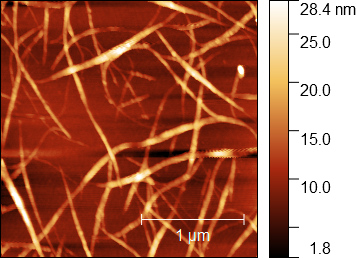
\includegraphics{figures/ch5/Ned_NTQ24_20220125_00235.png}

}

}

\subcaption{\label{fig-bundled-network}}
\end{minipage}%
%
\begin{minipage}[t]{0.05\linewidth}

{\centering 

~

}

\end{minipage}%
%
\begin{minipage}[t]{0.47\linewidth}

{\centering 

\raisebox{-\height}{

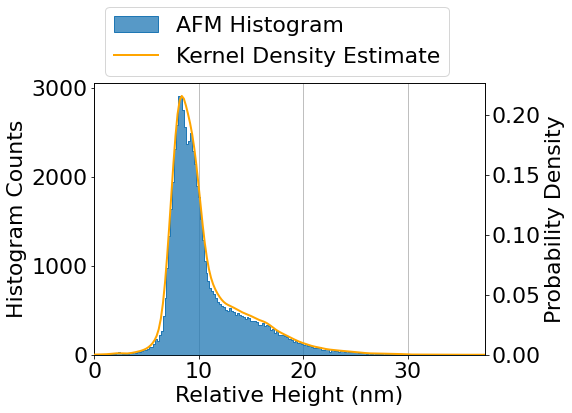
\includegraphics{figures/ch5/Ned_NTQ24_20220125_00235_histogram_initialguess.png}

}

}

\subcaption{\label{fig-bundled-network-histogram}}
\end{minipage}%
\newline
\begin{minipage}[t]{0.47\linewidth}

{\centering 

\raisebox{-\height}{

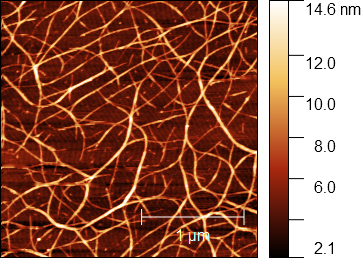
\includegraphics{figures/ch5/Ned_NTQ8C7_w4_pristine_00084_20210428(2).png}

}

}

\subcaption{\label{fig-dropcast-network}}
\end{minipage}%
%
\begin{minipage}[t]{0.05\linewidth}

{\centering 

~

}

\end{minipage}%
%
\begin{minipage}[t]{0.47\linewidth}

{\centering 

\raisebox{-\height}{

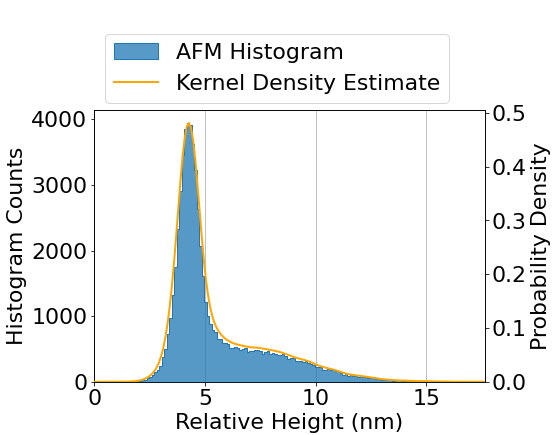
\includegraphics{figures/ch5/Ned_NTQ8C7_w4_pristine_00084_20210428(2)_histogram_initialguess.png}

}

}

\subcaption{\label{fig-dropcast-network-histogram}}
\end{minipage}%
\newline
\begin{minipage}[t]{0.47\linewidth}

{\centering 

\raisebox{-\height}{

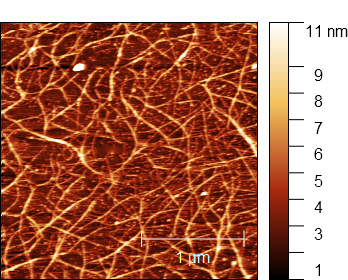
\includegraphics{figures/ch5/Ned_NGQ14D2_W4_pristine_20220713_00567.png}

}

}

\subcaption{\label{fig-steaming-network}}
\end{minipage}%
%
\begin{minipage}[t]{0.05\linewidth}

{\centering 

~

}

\end{minipage}%
%
\begin{minipage}[t]{0.47\linewidth}

{\centering 

\raisebox{-\height}{

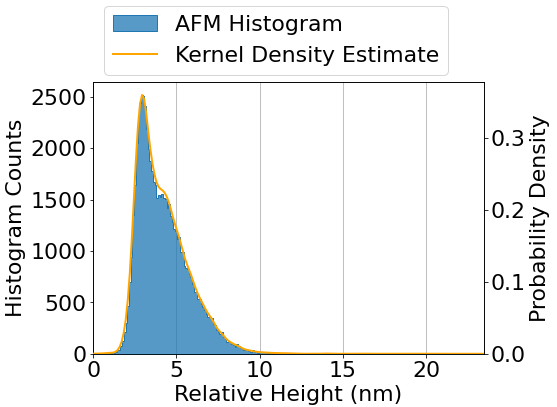
\includegraphics{figures/ch5/Ned_NGQ14D2_W4_pristine_20220713_00567_histogram_initialguess.png}

}

}

\subcaption{\label{fig-steaming-network-histogram}}
\end{minipage}%

\caption{\label{fig-afm-morphology}2.5 \(\mu\)m \(\times\) 2.5 \(\mu\)m
atomic force microscope (AFM) images of carbon nanotube films deposited
using various methods, shown side-by-side with histogram height
distributions and kernel density estimate (KDE) plots corresponding to
each image. The network shown in (a) with height distribution shown in
(b) was deposited in solvent, the network shown in (c) with height
distribution shown in (d) was dropcast in surfactant, and the network
shown in (e) with height distribution shown in (f) was dropcast in
surfactant with steam present.}

\end{figure}

It has previously been demonstrated that the diameter range of deposited
single-walled carbon nanotubes can be modelled via a normal or Gaussian
distribution \autocite{LeMieux2008,Liu2013,Vobornik2023}. However, when
we directly extract and bin the height profiles from the 2.5 \(\mu\)m
\(\times\) 2.5 \(\mu\)m AFM images, plotted in black in
Figure~\ref{fig-afm-morphology}, we obtain histograms which do not
follow a normal distribution. One reason for this result is the surface
roughness of the silicon dioxide substrate. The carbon nanotubes do not
lie perfectly level on a perfectly level silicon oxide substrate. In
practice, both the SiO\(_2\) substrate and the surface of the carbon
nanotubes both have a degree of roughness. To find the contribution of
surface roughness to the height profile histogram corresponding to each
network deposition method, silicon dioxide substrates were modified
using the same processes as in Figure~\ref{fig-afm-morphology} but
without carbon nanotubes present in the solutions used. 2.5 \(\mu\)m
\(\times\) 2.5 \(\mu\)m AFM images of the modified surfaces are shown in
Figure~\ref{fig-afm-substrate}.

\begin{figure}

\begin{minipage}[t]{0.47\linewidth}

{\centering 

\raisebox{-\height}{

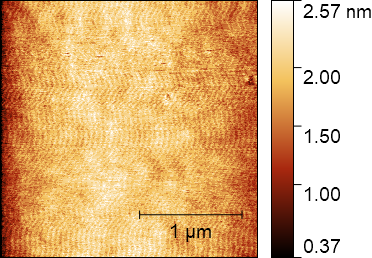
\includegraphics{figures/ch5/Ned_SiO2_00351_20231016.png}

}

}

\subcaption{\label{fig-sio2-only}}
\end{minipage}%
%
\begin{minipage}[t]{0.05\linewidth}

{\centering 

~

}

\end{minipage}%
%
\begin{minipage}[t]{0.47\linewidth}

{\centering 

\raisebox{-\height}{

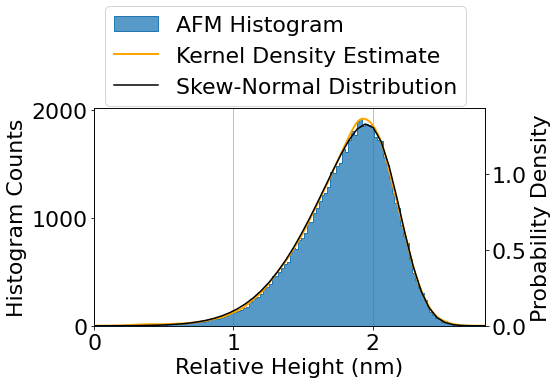
\includegraphics{figures/ch5/Ned_SiO2_00351_20231016_histogram_initialguess.png}

}

}

\subcaption{\label{fig-sio2-histogram}}
\end{minipage}%
\newline
\begin{minipage}[t]{0.47\linewidth}

{\centering 

\raisebox{-\height}{

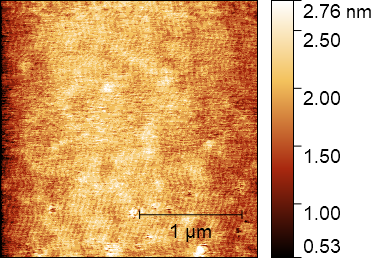
\includegraphics{figures/ch5/Ned_SiO2_s_surfactant_nosteam_00355_20231016.png}

}

}

\subcaption{\label{fig-surfactant-afm}}
\end{minipage}%
%
\begin{minipage}[t]{0.05\linewidth}

{\centering 

~

}

\end{minipage}%
%
\begin{minipage}[t]{0.47\linewidth}

{\centering 

\raisebox{-\height}{

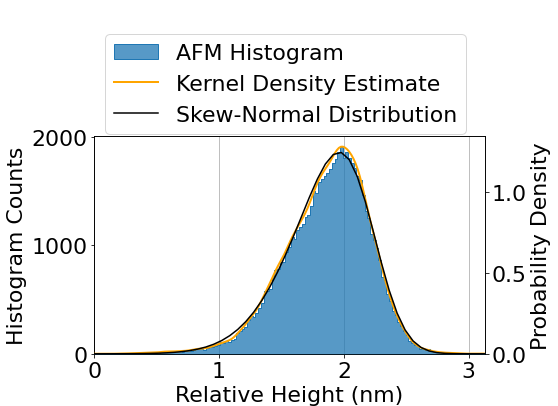
\includegraphics{figures/ch5/Ned_SiO2_s_surfactant_nosteam_00355_20231016_histogram_initialguess.png}

}

}

\subcaption{\label{fig-surfactant-histogram}}
\end{minipage}%
\newline
\begin{minipage}[t]{0.47\linewidth}

{\centering 

\raisebox{-\height}{

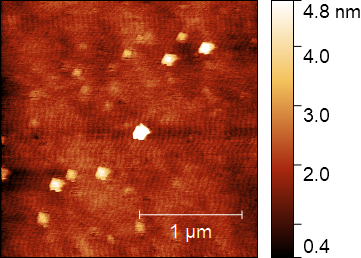
\includegraphics{figures/ch5/Ned_SiO2_s_surfactant_steam_00357_20231016.png}

}

}

\subcaption{\label{fig-steamed-surfactant}}
\end{minipage}%
%
\begin{minipage}[t]{0.05\linewidth}

{\centering 

~

}

\end{minipage}%
%
\begin{minipage}[t]{0.47\linewidth}

{\centering 

\raisebox{-\height}{

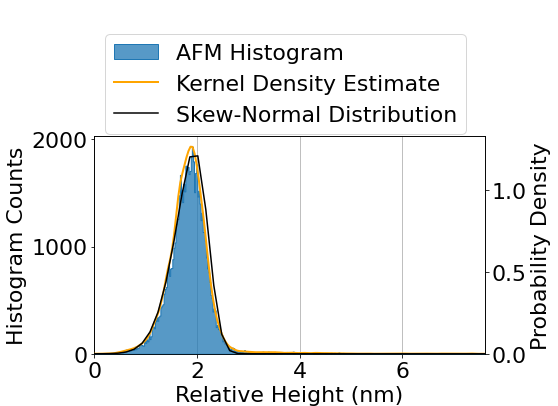
\includegraphics{figures/ch5/Ned_SiO2_s_surfactant_steam_00357_20231016_histogram_initialguess.png}

}

}

\subcaption{\label{fig-steamed-surfactant-histogram}}
\end{minipage}%

\caption{\label{fig-afm-substrate}2.5 \(\mu\)m \(\times\) 2.5 \(\mu\)m
atomic force microscope (AFM) images of silicon dioxide substrates
alongside histogram height distributions and KDE plots corresponding to
each image. The substrate in (a) and (b) was exposed to solvent, the
substrate in (c) and (d) was exposed to surfactant, and the substrate in
(e) and (f) was exposed to surfactant with steam present.}

\end{figure}

In Figure~\ref{fig-afm-substrate}, we see that each substrate surface
has a roughness that follows a normal distribution with some degree of
skewness. Figure~\ref{fig-sio2-histogram} and
Figure~\ref{fig-surfactant-histogram} are negatively skewed
distributions. The fitted skew-normal distribution in
Figure~\ref{fig-sio2-histogram} has a skew parameter \(\alpha\) (or
shape parameter) of -3.2, a location parameter \(\xi\) of 2.2 nm and a
scale parameter \(\omega\) of 0.5 nm, while in
Figure~\ref{fig-surfactant-histogram} \(\alpha = -2.2\), \(\xi = 2.2\)
nm and \(\omega = 0.5\) nm. \(\xi\) and \(\omega\) correspond to the
mean and standard deviation of the skew-free normal distribution when
\(\alpha\) is set equal to zero \autocite{Azzalini1999}. The close
correspondence between \(\xi\) and \(\omega\) for these distributions
but not \(\alpha\) implies that the skewness is a variable imaging or
processing artifact rather than a physical property of the surface.
Without distortion, the roughness of a clean SiO\(_2\) surface should
follow a normal distribution \autocite{Velicky2015}.

However, Figure~\ref{fig-steamed-surfactant-histogram} has a pronounced
positive skew with a long tail. The tail appears to result from the
contribution of residual surfactant to surface morphology, observed in
Figure~\ref{fig-steamed-surfactant} and discussed elsewhere in the
literature \autocite{Vobornik2023}. Attempting to fit a skew-normal
distribution to this histogram fails when all three variables are
allowed to vary due to the presence of the tail. Instead, we fix \(\xi\)
and \(\omega\) at 2.2 nm and 0.5 nm respectively to mimic the silicon
dioxide distributions previously obtained, and only \(\alpha\) is
allowed to vary during the fitting process. The result is shown in
Figure~\ref{fig-steamed-surfactant-histogram}. The fitted distribution
has an \(\alpha\) of -2.4. The distribution closely fits the negative
tail of the histogram, but deviates slightly from the positive tail due
to the presence of surfactant. Since this deviation is small, the
quality of the fit is still reasonably high, with an R-squared value of
0.98. Surfactant contamination could have negative effects on both
sensitivity of carbon nanotubes and also could damage attached
biological elements.

\begin{figure}

\begin{minipage}[t]{0.47\linewidth}

{\centering 

\raisebox{-\height}{

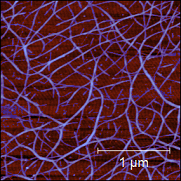
\includegraphics{figures/ch5/Ned_NTQ8C7_w4_pristine_00084_20210428(2)_mask.png}

}

}

\subcaption{\label{fig-mask}}
\end{minipage}%
%
\begin{minipage}[t]{0.05\linewidth}

{\centering 

~

}

\end{minipage}%
%
\begin{minipage}[t]{0.47\linewidth}

{\centering 

\raisebox{-\height}{

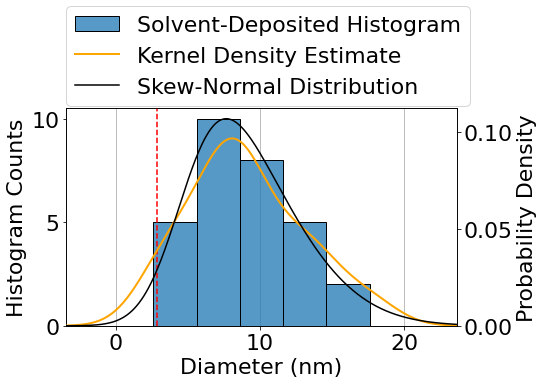
\includegraphics{figures/ch5/NTQ24_20220125_00235_cnt_histogram.png}

}

}

\subcaption{\label{fig-solvent-cnt-histogram}}
\end{minipage}%
\newline
\begin{minipage}[t]{0.47\linewidth}

{\centering 

\raisebox{-\height}{

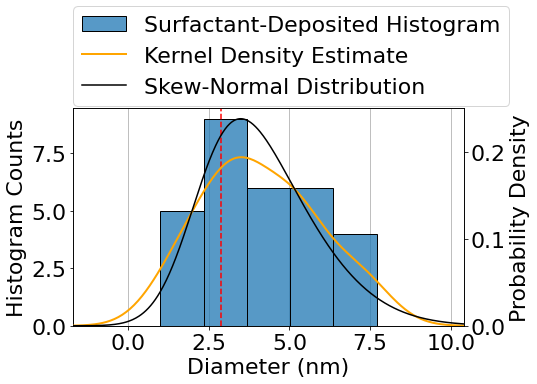
\includegraphics{figures/ch5/NTQ8C7_w4_pristine_cnt_histogram.png}

}

}

\subcaption{\label{fig-surfactant-cnt-histogram}}
\end{minipage}%
%
\begin{minipage}[t]{0.05\linewidth}

{\centering 

~

}

\end{minipage}%
%
\begin{minipage}[t]{0.47\linewidth}

{\centering 

\raisebox{-\height}{

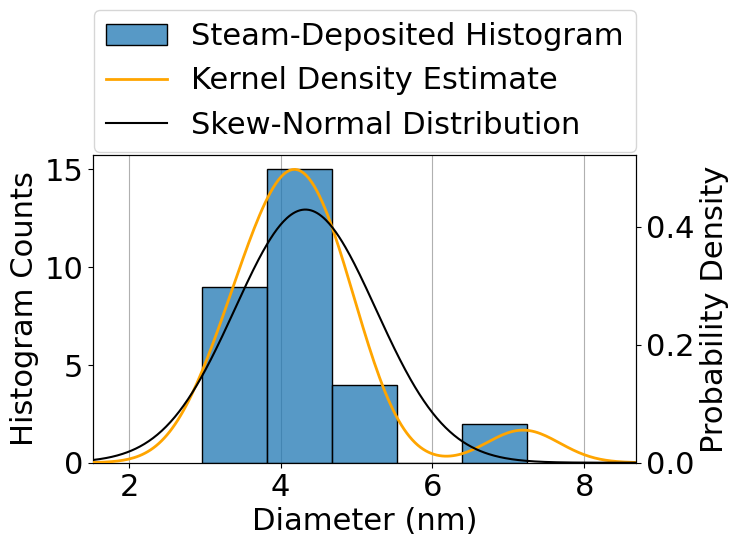
\includegraphics{figures/ch5/NT14D2_W4_pristine_cnt_histogram.png}

}

}

\subcaption{\label{fig-steamed-surfactant-cnt-histogram}}
\end{minipage}%

\caption{\label{fig-cnt-histogram}An masked AFM image is shown in (a),
where the masked carbon nanotube bundles are shaded blue. The mask sets
a height threshold so that masked features are excluded from the height
dataset. Histogram height distributions with corresponding KDE plots
collected via the morphology analysis method outlined by Vobornik
\emph{et al.} \autocite{Vobornik2023} are shown in (b)-(d). The
substrate in (b) was exposed to solvent, the substrate in (c) was
exposed to surfactant, and the substrate in (d) was exposed to
surfactant with steam present.}

\end{figure}

Using the morphology analysis technique outlined by Vobornik \emph{et
al.} \autocite{Vobornik2023}, we collected five successive diameter
measurements of 30 carbon nanotube bundles using Gwyddion. Measurements
were not taken at bundle junctions. A height threshold `mask' was
defined in Gwyddion to determine average substrate height, as shown in
Figure~\ref{fig-mask}. This background value was subtracted from our
diameter measurements to determine the actual bundle height. The means
of the solvent-deposited, surfactant-deposited and steam-assisted
surfactant-deposited bundle diameter histograms are \(8.8 \pm 4.0\) nm,
\(4.2 \pm 1.8\) nm and \(3.3 \pm 1.0\) nm respec tively. We see that an
increased maximum feature height leads to an increased mean background
height, and by examining the AFM images in
Figure~\ref{fig-afm-morphology} we see that this may be due to deep
artifacts on the surface of the substrate in the vicinity of large
features. The average of the five height-adjusted values for each carbon
nanotube bundle was then calculated, and these 30 averages were sorted
into six equal-sized bins. The binned bundle diameter measurements,
alongside estimated probability density, are shown in
Figure~\ref{fig-cnt-histogram}.

We notice from Figure~\ref{fig-cnt-histogram} that each histogram
appears to follow a positively skewed normal distribution, different to
the skew-free normal distribution we expect from previous works
\autocite{LeMieux2008,Liu2013,Vobornik2023}. The skew is likely another
artifact from imaging the network with the atomic force microscope. The
force of the atomic force microscope tip is known to cause larger
bundles to undergo some degree of compression, and the resulting
systematic underestimation of their height may be responsible for the
distribution skewness \autocite{Vobornik2023}. The fitted skew-normal
distribution in Figure~\ref{fig-solvent-cnt-histogram} has
\(\alpha = 2.7\), \(\xi = 4.3\) nm, \(\omega = 5.9\) nm, the
distribution in Figure~\ref{fig-surfactant-cnt-histogram} has
\(\alpha = 2.4\), \(\xi = 2.2\) nm, \(\omega = 2.6\) nm, and the
distribution in Figure~\ref{fig-steamed-surfactant-cnt-histogram} has
\(\alpha = 3.6\), \(\xi = 2.2\) nm and \(\omega = 1.5\) nm. We notice
that the probability density for the carbon nanotube bundle histogram
drops to approximately zero at or before 0 nm, as is physically
appropriate.

\hypertarget{tbl-circle-packing}{}
\begin{longtable}[]{@{}
  >{\raggedright\arraybackslash}p{(\columnwidth - 16\tabcolsep) * \real{0.1053}}
  >{\raggedright\arraybackslash}p{(\columnwidth - 16\tabcolsep) * \real{0.1228}}
  >{\raggedright\arraybackslash}p{(\columnwidth - 16\tabcolsep) * \real{0.0965}}
  >{\raggedright\arraybackslash}p{(\columnwidth - 16\tabcolsep) * \real{0.0965}}
  >{\raggedright\arraybackslash}p{(\columnwidth - 16\tabcolsep) * \real{0.1228}}
  >{\raggedright\arraybackslash}p{(\columnwidth - 16\tabcolsep) * \real{0.1228}}
  >{\raggedright\arraybackslash}p{(\columnwidth - 16\tabcolsep) * \real{0.1228}}
  >{\raggedright\arraybackslash}p{(\columnwidth - 16\tabcolsep) * \real{0.1228}}
  >{\raggedright\arraybackslash}p{(\columnwidth - 16\tabcolsep) * \real{0.0877}}@{}}
\caption{\label{tbl-circle-packing}The first eight optimised ratios of
2D packed circle diameter to encompassing circle diameter, given to 3
s.f. (encompassing circle diameter = \(d\), number of packed circles =
\(n\), approximate packed circle diameter = \(d_n\)).\\
}\tabularnewline
\toprule\noalign{}
\endfirsthead
\endhead
\bottomrule\noalign{}
\endlastfoot
\(n\) & \text{2} & \text{3} & \text{4} & \text{5} & \text{6} & \text{7}
& \text{8} & \text{9} \\
\(d\)/\(d_n\) & \text{2.00} & 2.15 & 2.41 & \text{2.70} & \text{3.00} &
\text{3.00} & \text{3.30} & 3.61 \\
\end{longtable}

\hypertarget{tbl-histogram-parameters}{}
\begin{table}
\caption{\label{tbl-histogram-parameters}The mean of histogram distributions for carbon nanotube films deposited
using various methods, alongside estimates for the number of nanotubes
present per mean bundle and the estimated proportion of multi-tubed
bundles present across the network. }\tabularnewline

\centering
\begin{tabular}{>{\raggedright\arraybackslash}p{4cm}>{\centering\arraybackslash}p{3cm}>{\centering\arraybackslash}p{3cm}>{\centering\arraybackslash}p{3cm}}
\toprule
 & Mean Bundle Diameter (nm) & Tubes per Average Bundle & \% Multi-Tube Bundles\\
\midrule
Solvent deposited & 8.8 ± 4.0 & 28 & > 96\%\\
Surfactant deposited & 4.2 ± 1.8 & 5 & > 75\%\\
Surfactant deposited with steam & 3.3 ± 1.0 & 3 & > 65\%\\
\bottomrule
\end{tabular}
\end{table}

If we model carbon nanotube bundles as cylinders, and we assume the
component nanotubes follow 2D packing and are of equal diameter, we can
state the mean bundle size for each deposition type in terms of number
of nanotubes \emph{n} \autocite{Graham1998,Murugathas2018,Specht2023}.
Table~\ref{tbl-circle-packing} shows the relationship between the
diameter of a bundle and the constituent diameters of up to nine 2D
packed carbon nanotubes within that bundle. Assuming an average carbon
nanotube diameter of 1.45 nm, we can use the \(d\)/\(d_n\) packing
ratios to obtain an estimate of the number of nanotubes in the mean
bundle size for each deposition \autocite{Specht2023}. These estimates
are shown in Table~\ref{tbl-histogram-parameters}. Also shown in
Table~\ref{tbl-histogram-parameters} is an estimate of the ratio of
single- to multi-tube bundles for each deposition. This estimate was
obtained by taking the integral of each distribution with a lower bound
of 2.9 nm, the minimum multi-tube bundle size for 1.45 nm diameter
nanotubes. As the area under the curve represents the probability a
bundle will have a particular diameter, this integral should give a good
estimate of the relative proportion of multi-tube bundles.
Table~\ref{tbl-histogram-parameters} should be interpreted as
lower-limit estimates of the size and relative proportion of bundles,
recalling that the distribution skewness indicates underestimation of
the true bundle height.

Both the carbon nanotube bundle diameter mean and standard deviation are
small for surfactant-deposited films when compared to the mean and
standard deviation of solvent-deposited films. However, despite the
presence of surfactant, it is apparent both from
Figure~\ref{fig-afm-morphology} and Table~\ref{tbl-histogram-parameters}
that not all surfactant-dispersed carbon nanotubes are deposited
individually. Bundling may occur during the process of deposition onto
the substrate, which could disrupt the repulsive forces from the
surfactant coating and allow attractive forces to temporarily dominate.
It is possible that the bundling of surfactant-dispersed carbon
nanotubes is a consequence of dynamics introduced by the coffee-ring
effect \autocite{Deegan1997,VanGaalen2021}. The coffee-ring effect
refers to a build-up of dispersed solid forming around the edges of a
dispersion evaporating on a surface. This process occurs due to the
dispersion edges being fixed by surface forces, leading to capillary
flow outwards to replace liquid evaporating at the edges, bringing solid
material along with it. The presence of vapour is known to disrupt this
capillary effect \autocite{Bishop2020}, which may explain why mean
bundle diameter is lower for the films deposited in surfactant with
steam present relative to films deposited in surfactant without steam.

From this discussion, we can conclude that the histograms shown in
Figure~\ref{fig-afm-morphology} are linear combinations of skewed normal
distributions corresponding to both the substrate surface, with a
negative skew, and the carbon nanotube bundles, with a positive skew. X
and Y junctions between overlapping nanotubes may also form a similarly
skewed normal distribution as part of the full histogram
\autocite{Murugathas2018}. The complete linear combination could be
modelled mathematically in order to rapidly extract key parameters from
atomic force microscope images \autocite{Marchenko2010}, but
implementing this approach is outside of the scope of this thesis. The
prevalence of carbon nanotube bundling on the surface is lowered by the
presence of surfactant during deposition. Introducing steam when
depositing with surfactant lowers bundling even further, but also leads
to residual surfactant pooling and attaching to the substrate surface.
These results may both be explained by the presence of steam enabling
surfactant to follow carbon nanotubes to the substrate surface, which
keeps them from bundling during the attachment process. The unwanted
persistence of surfactant means that further vacuum annealing may be
required for robust biosensors \autocite{Kane2014}.

\hypertarget{sec-pristine-raman}{%
\subsection{Raman Spectroscopy}\label{sec-pristine-raman}}

\begin{figure}

\begin{minipage}[t]{0.47\linewidth}

{\centering 

\raisebox{-\height}{

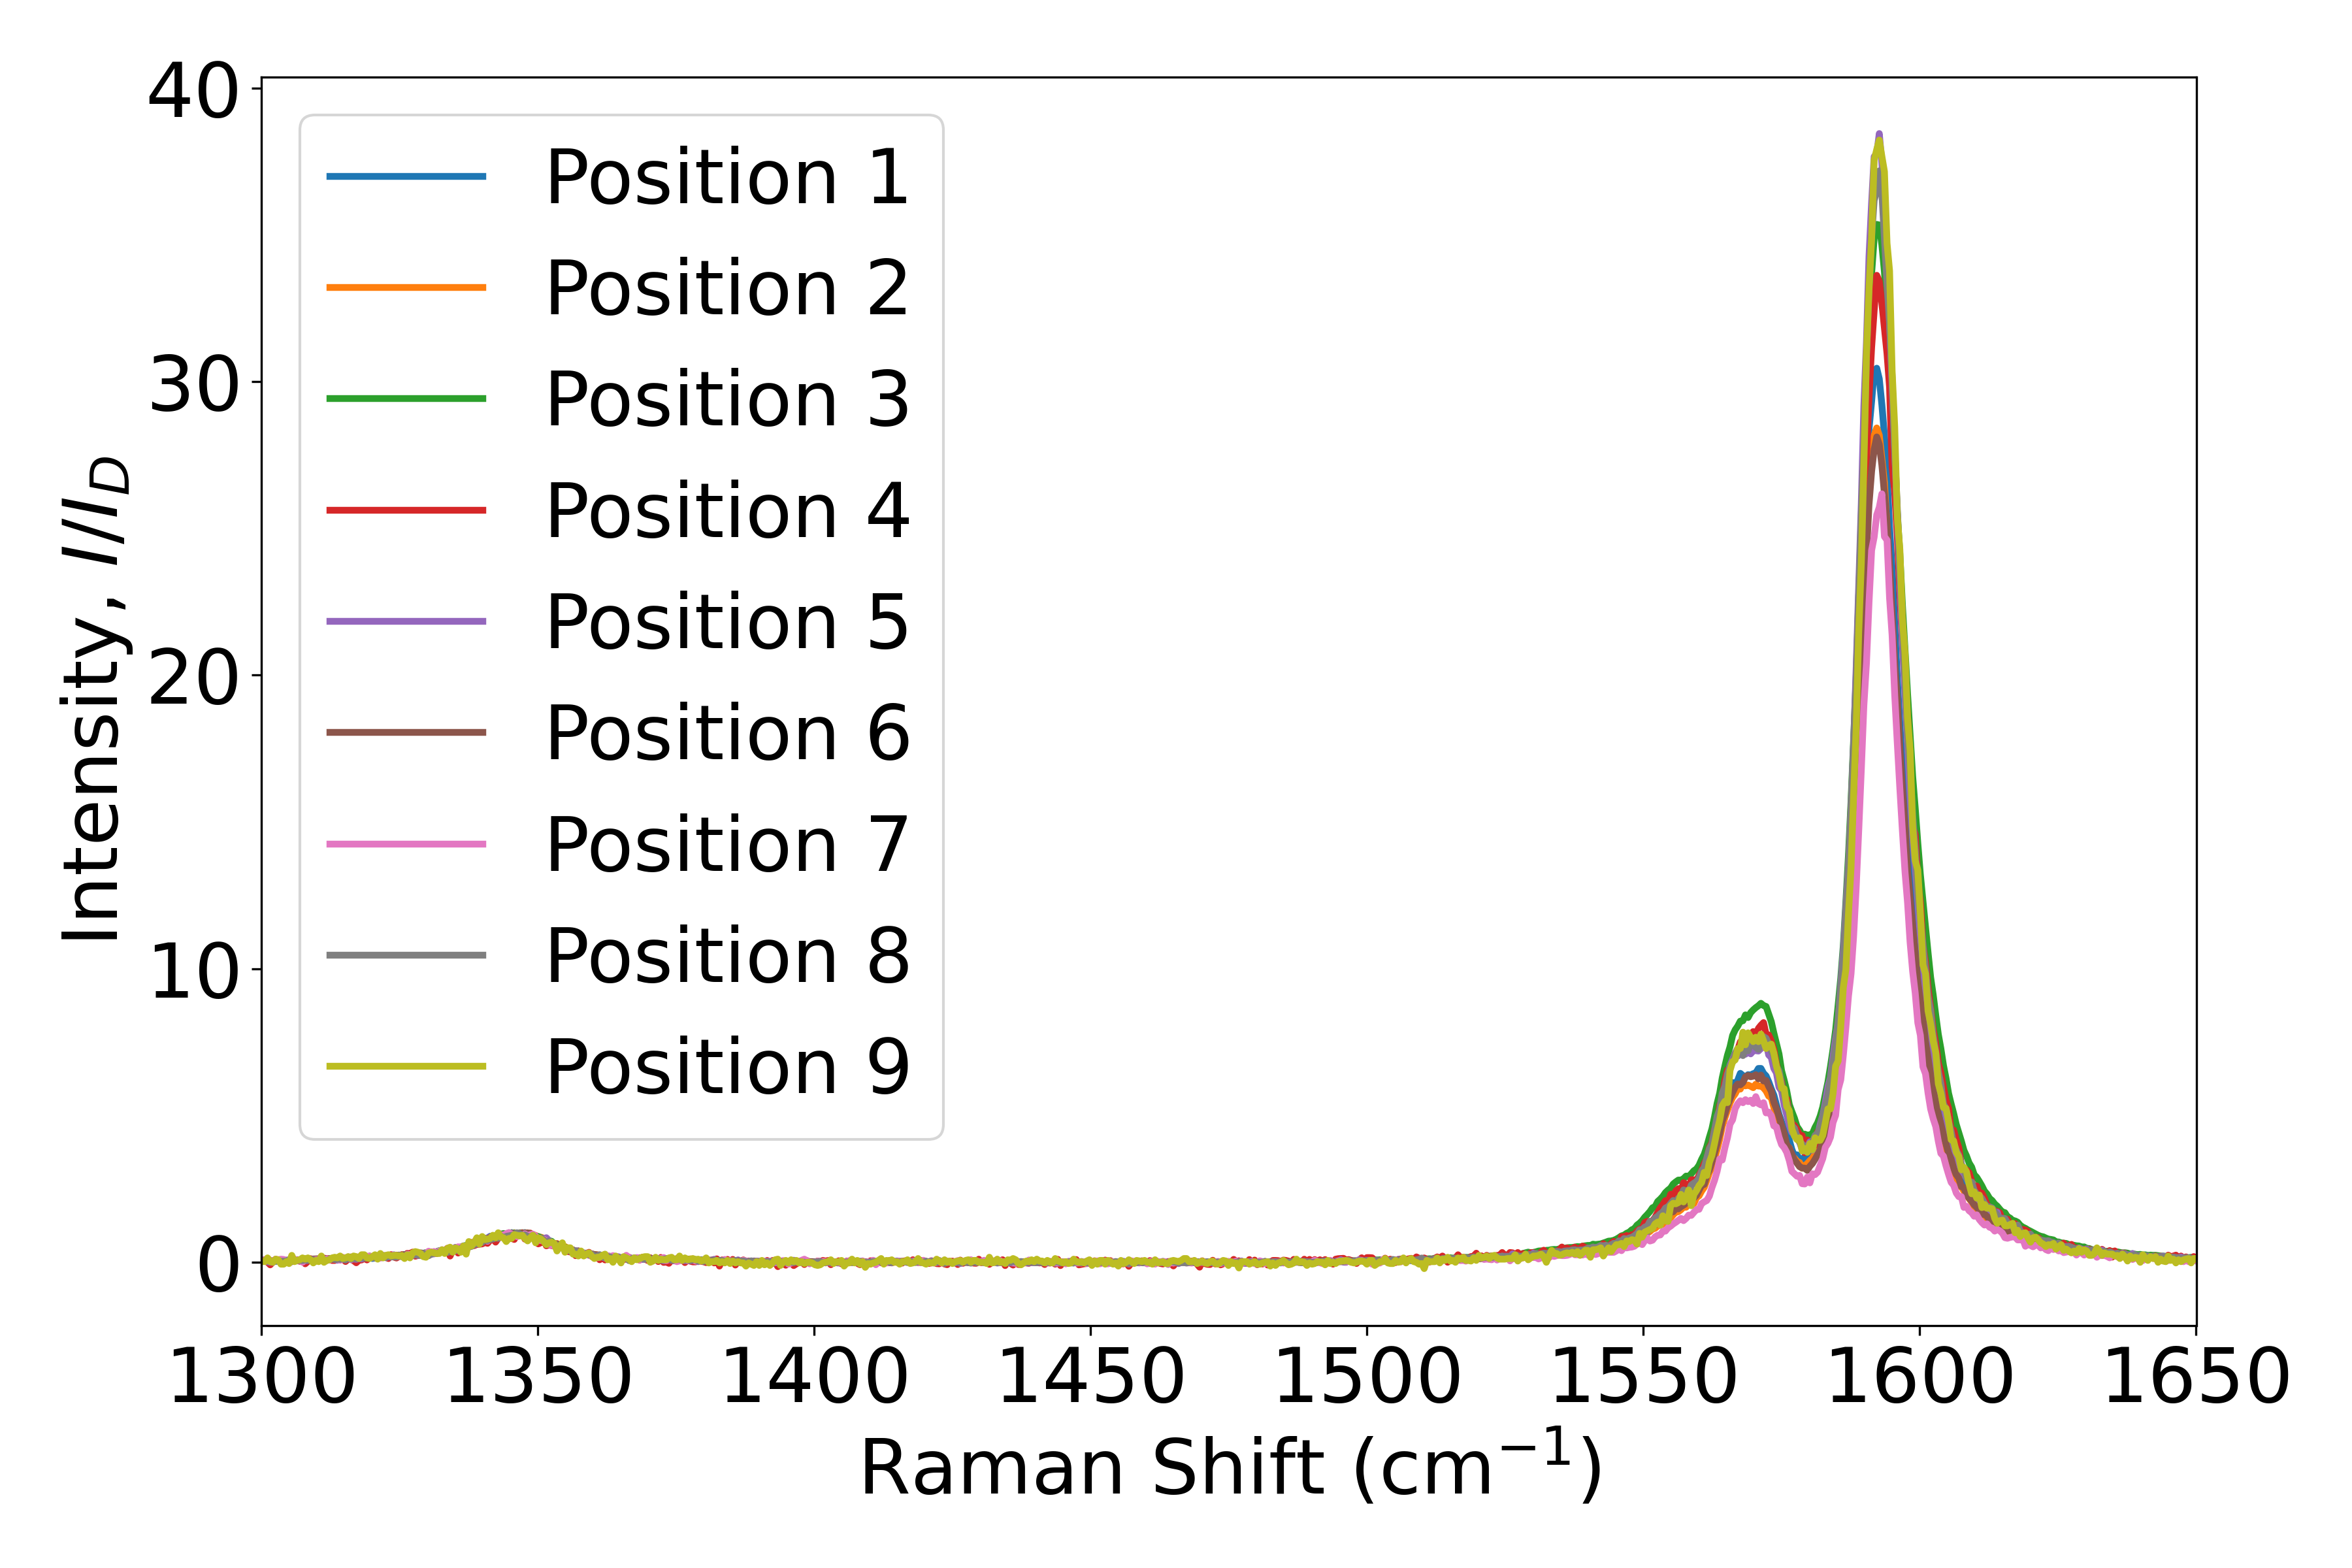
\includegraphics{figures/ch5/raman_bundled.png}

}

}

\subcaption{\label{fig-solvent-deposited}}
\end{minipage}%
%
\begin{minipage}[t]{0.05\linewidth}

{\centering 

~

}

\end{minipage}%
%
\begin{minipage}[t]{0.47\linewidth}

{\centering 

\raisebox{-\height}{

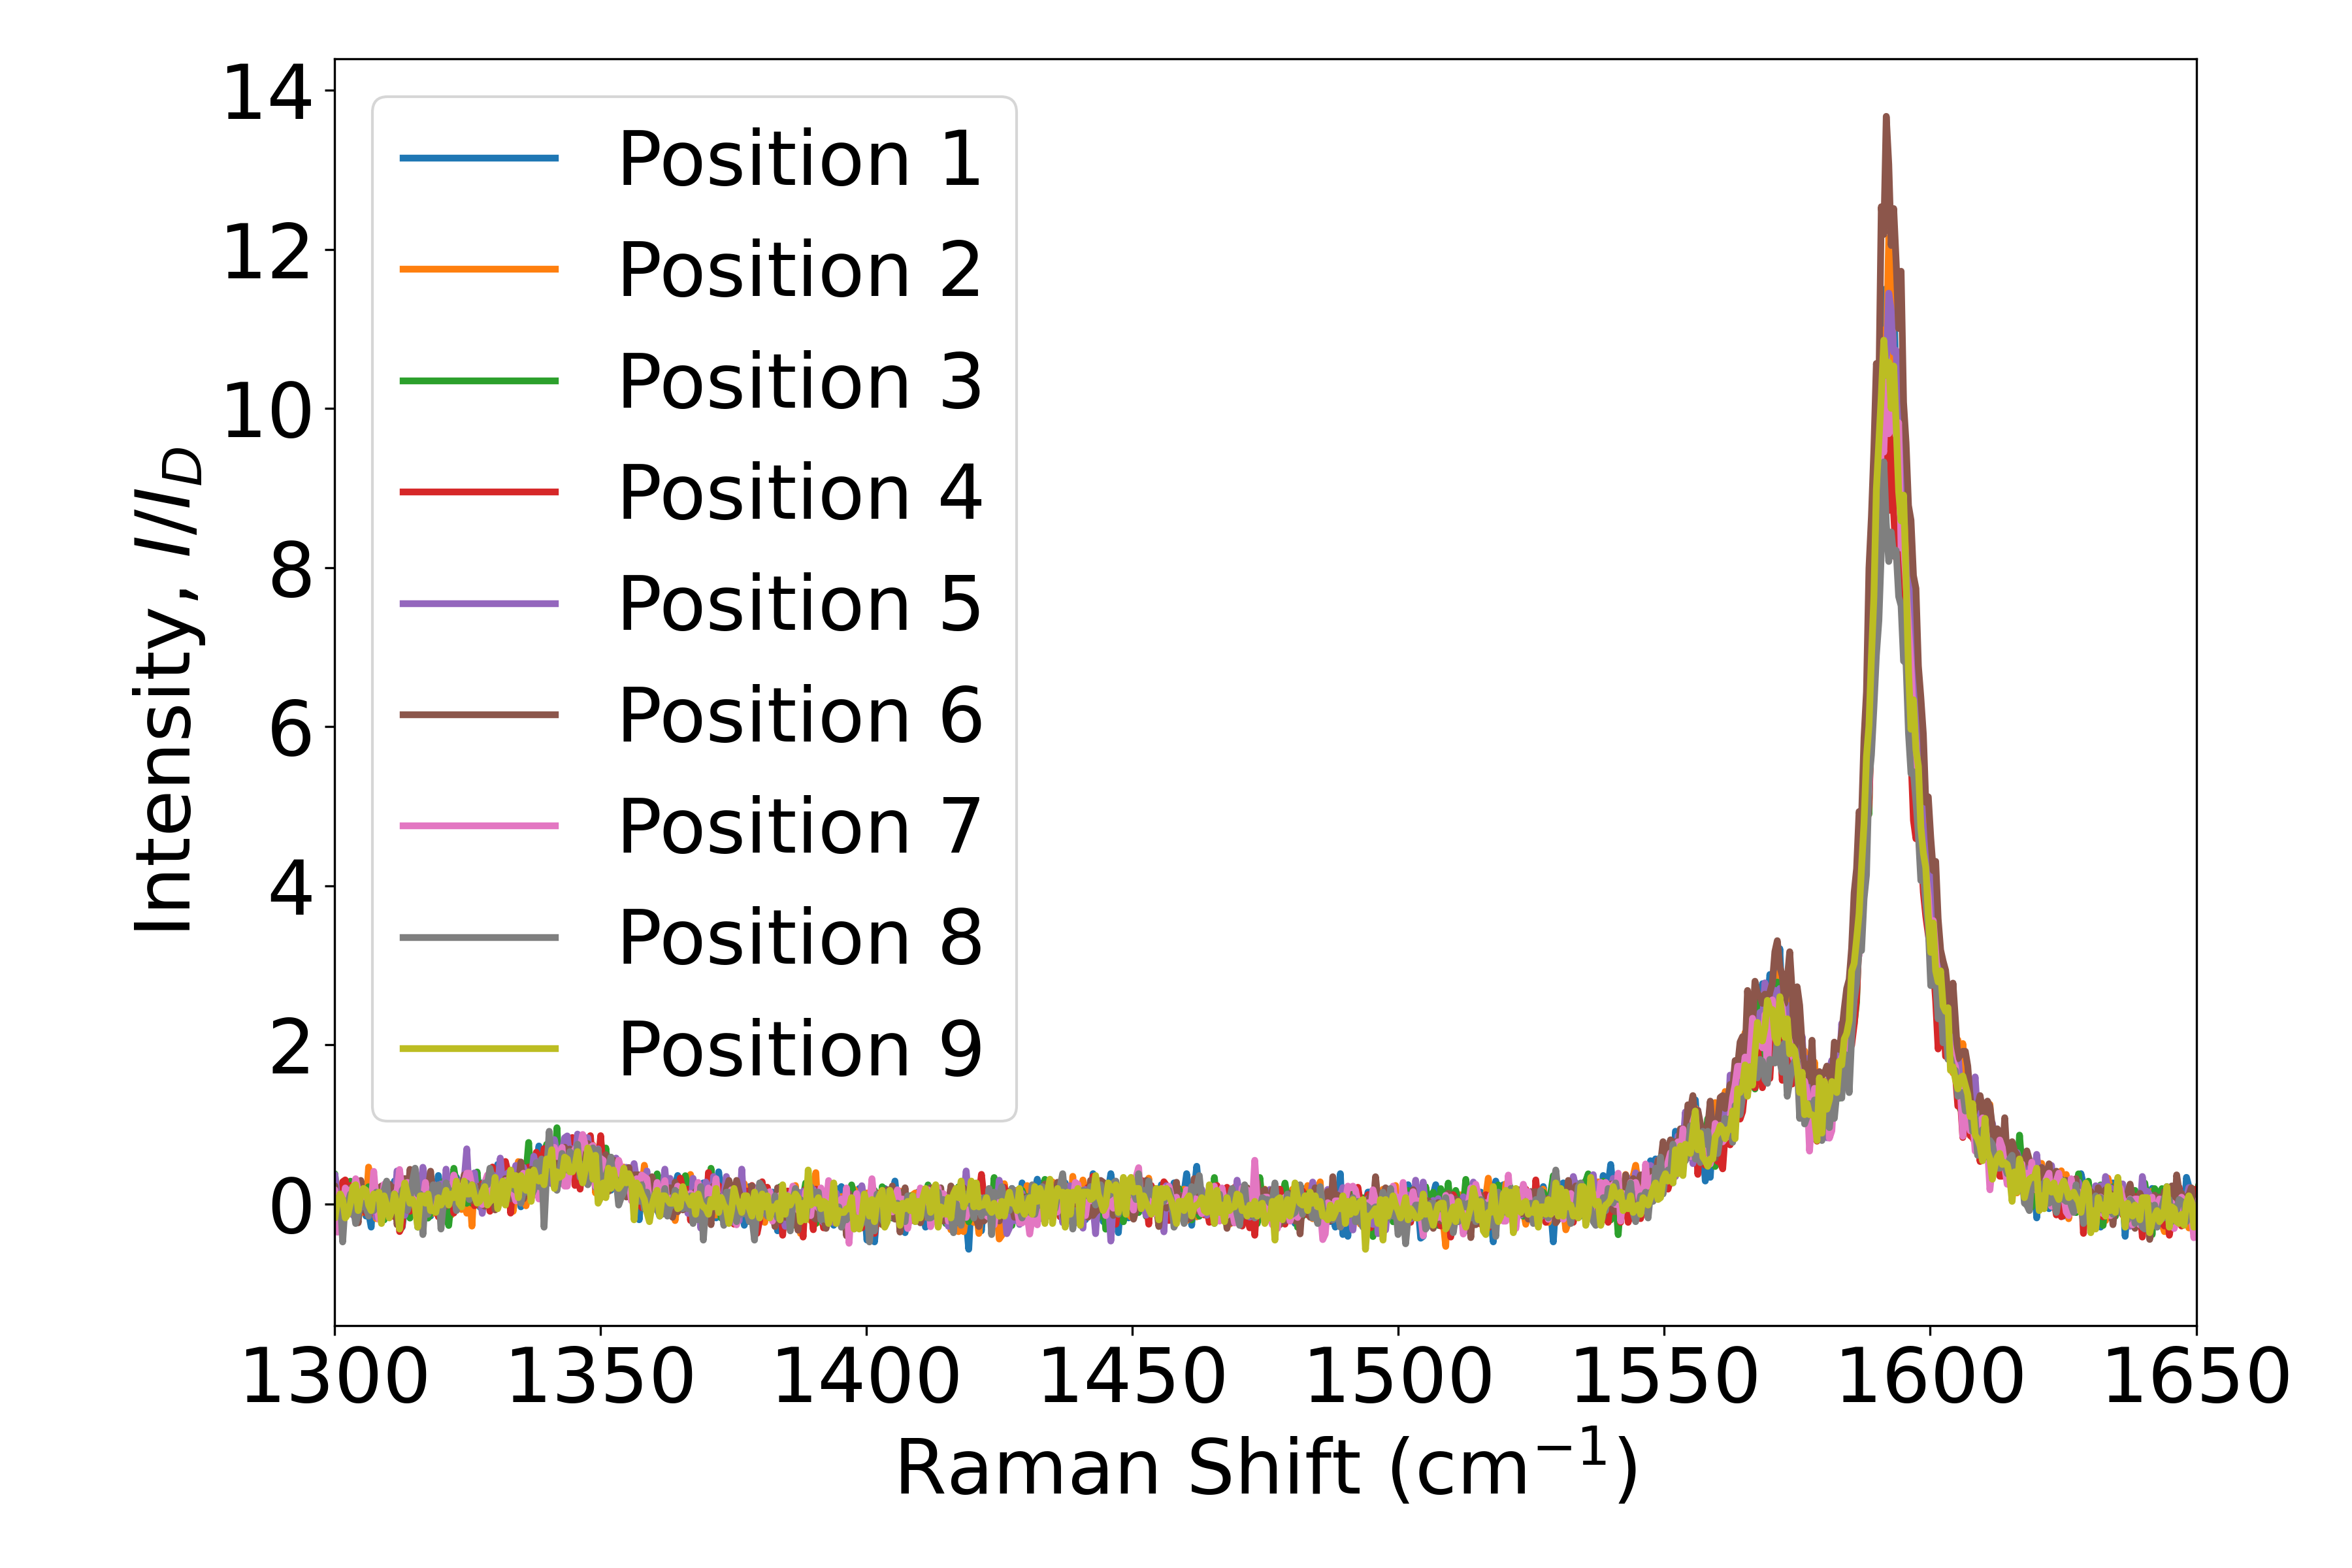
\includegraphics{figures/ch5/raman_singletubes.png}

}

}

\subcaption{\label{fig-surfactant-deposited}}
\end{minipage}%

\caption{\label{fig-pristine-raman}A series of nine Raman spectra at
different locations across a 10 \(\mu\)m \(\times\) 50 \(\mu\)m carbon
nanotube film region, spaced at least 10 \(\mu\)m apart, with (a)
showing spectra from a film deposited in solvent and (b) showing spectra
from a film deposited in surfactant with steam present.}

\end{figure}

\hypertarget{sec-pristine-electrical-characterisation}{%
\section{Electrical Characteristics of Pristine
Devices}\label{sec-pristine-electrical-characterisation}}

\hypertarget{carbon-nanotube-network-devices}{%
\subsection{Carbon Nanotube Network
Devices}\label{carbon-nanotube-network-devices}}

\begin{figure}

\begin{minipage}[t]{0.49\linewidth}

{\centering 

\raisebox{-\height}{

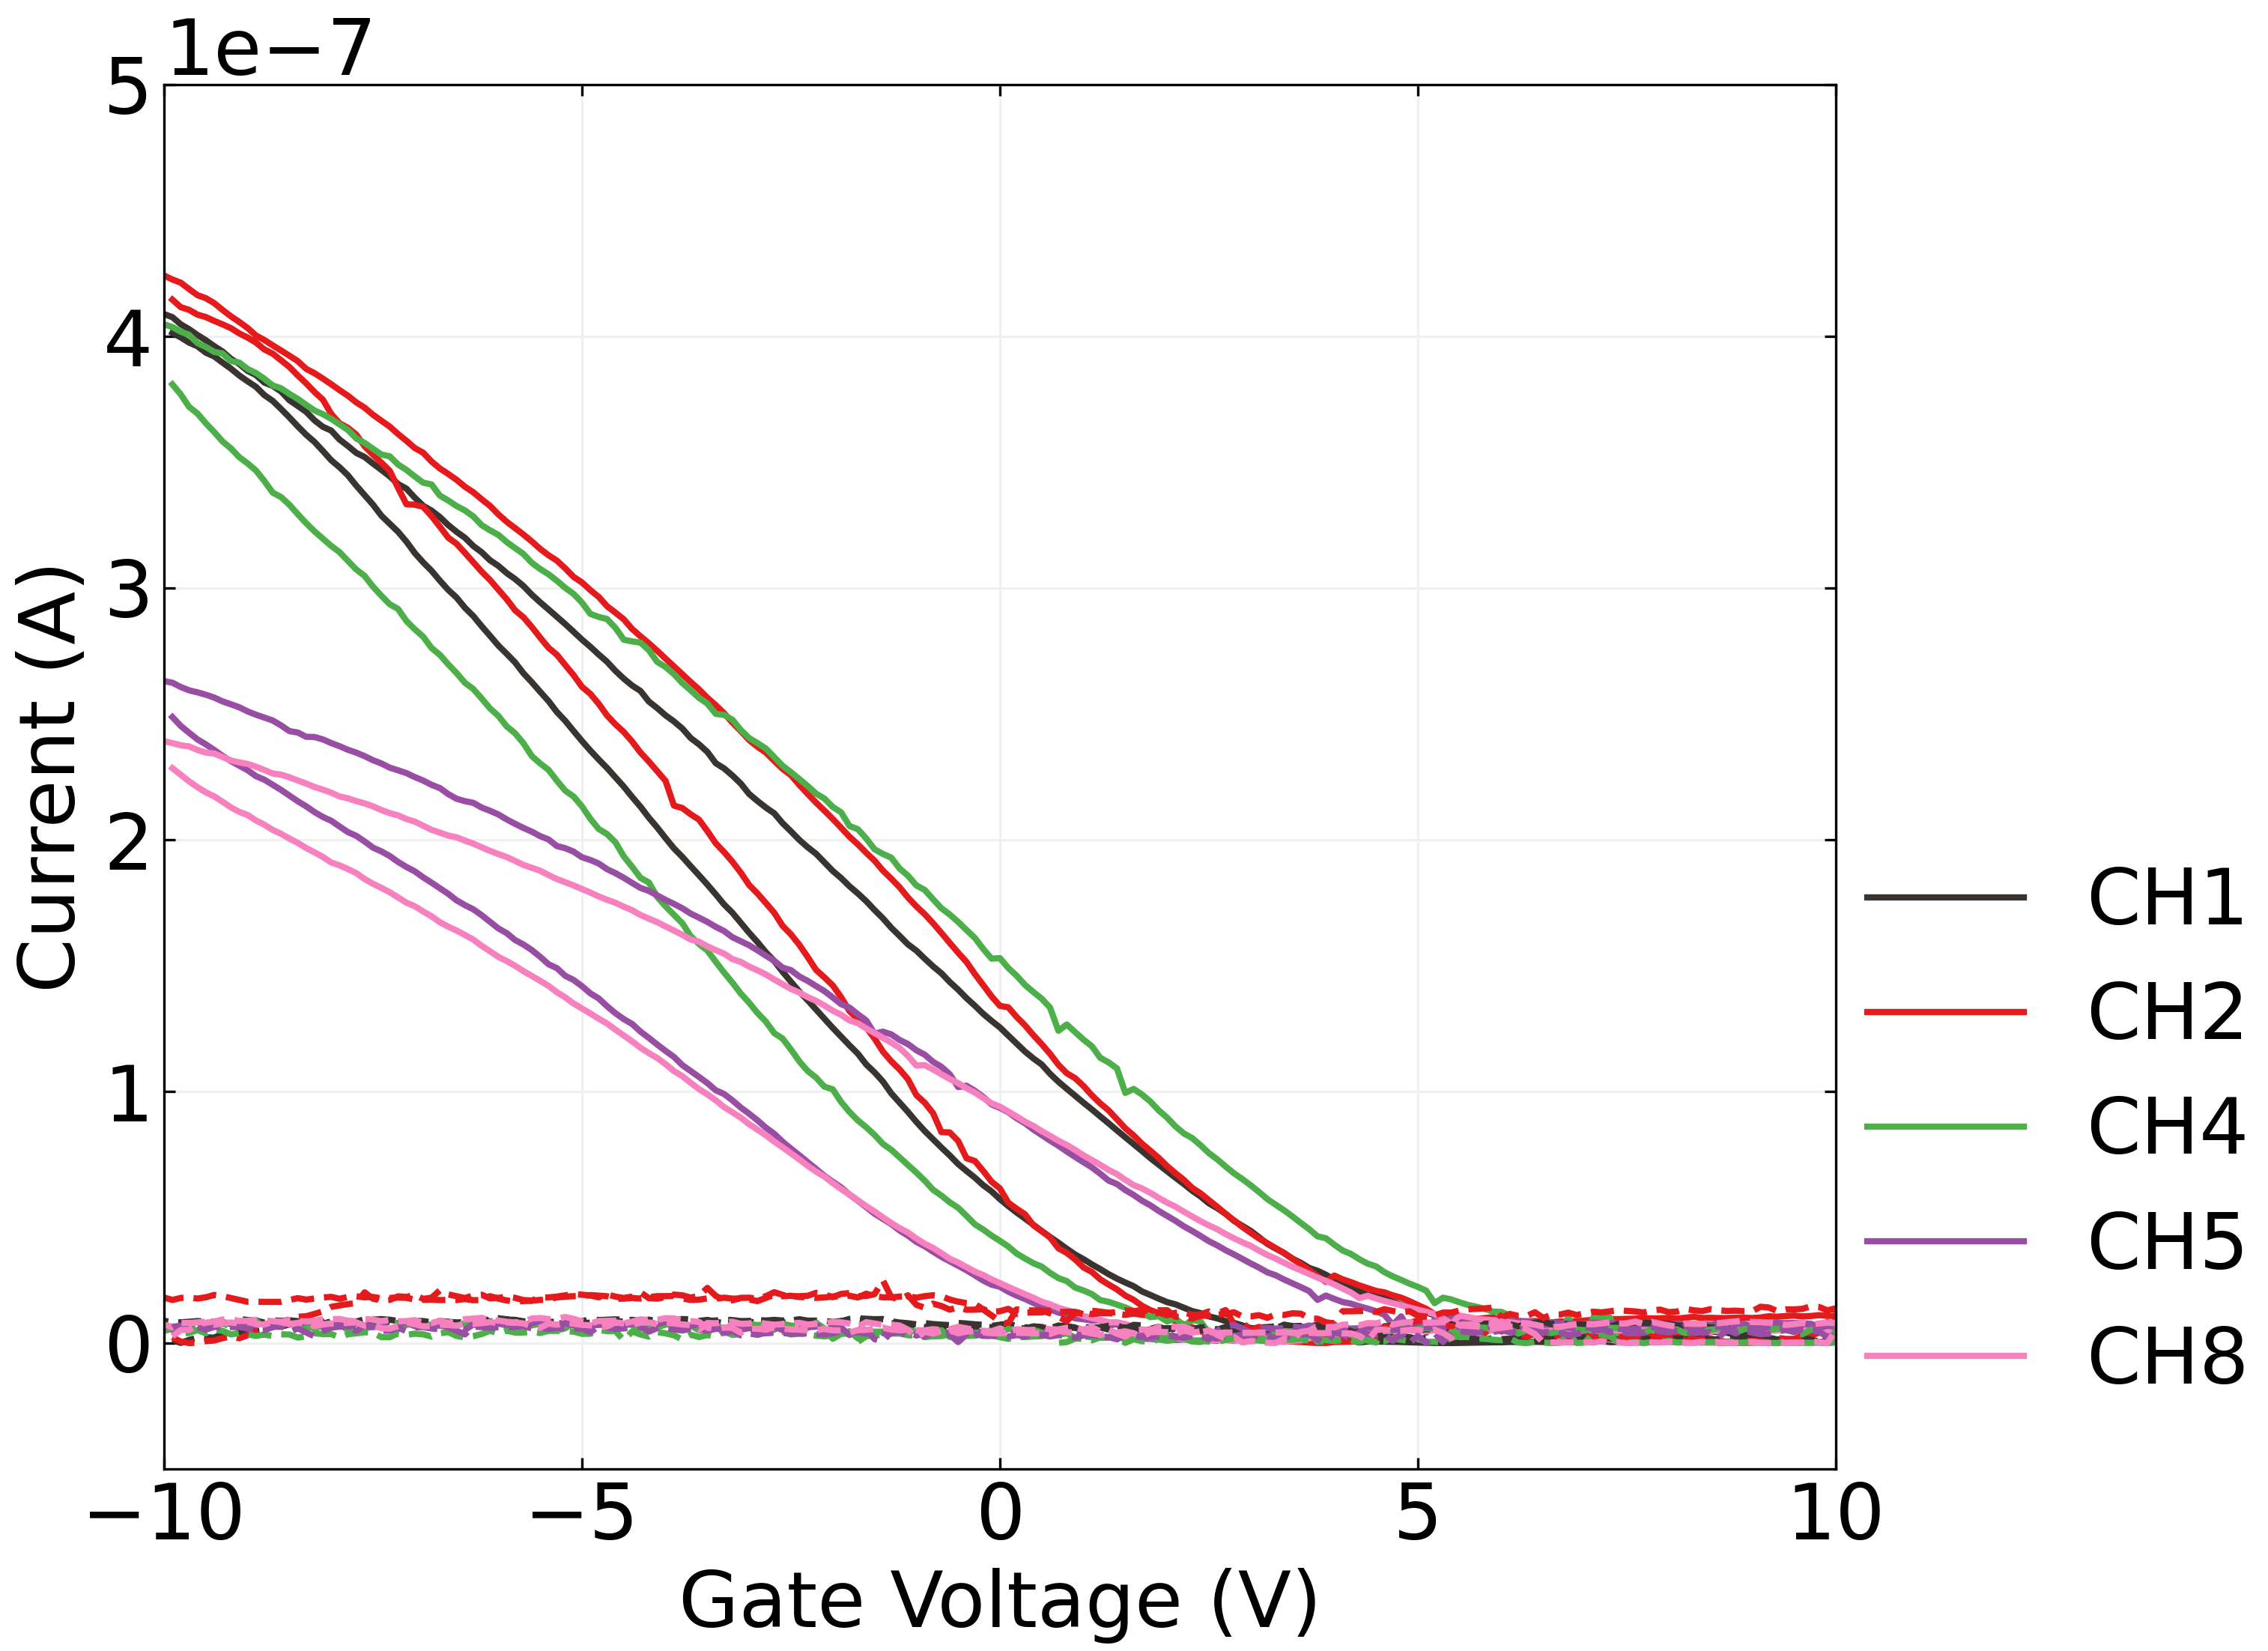
\includegraphics{figures/ch5/NTQ22C2_solvent_backgate.png}

}

}

\subcaption{\label{fig-solvent-tx-bg}Solvent-based deposition,
back-gated}
\end{minipage}%
%
\begin{minipage}[t]{0.02\linewidth}

{\centering 

~

}

\end{minipage}%
%
\begin{minipage}[t]{0.49\linewidth}

{\centering 

\raisebox{-\height}{

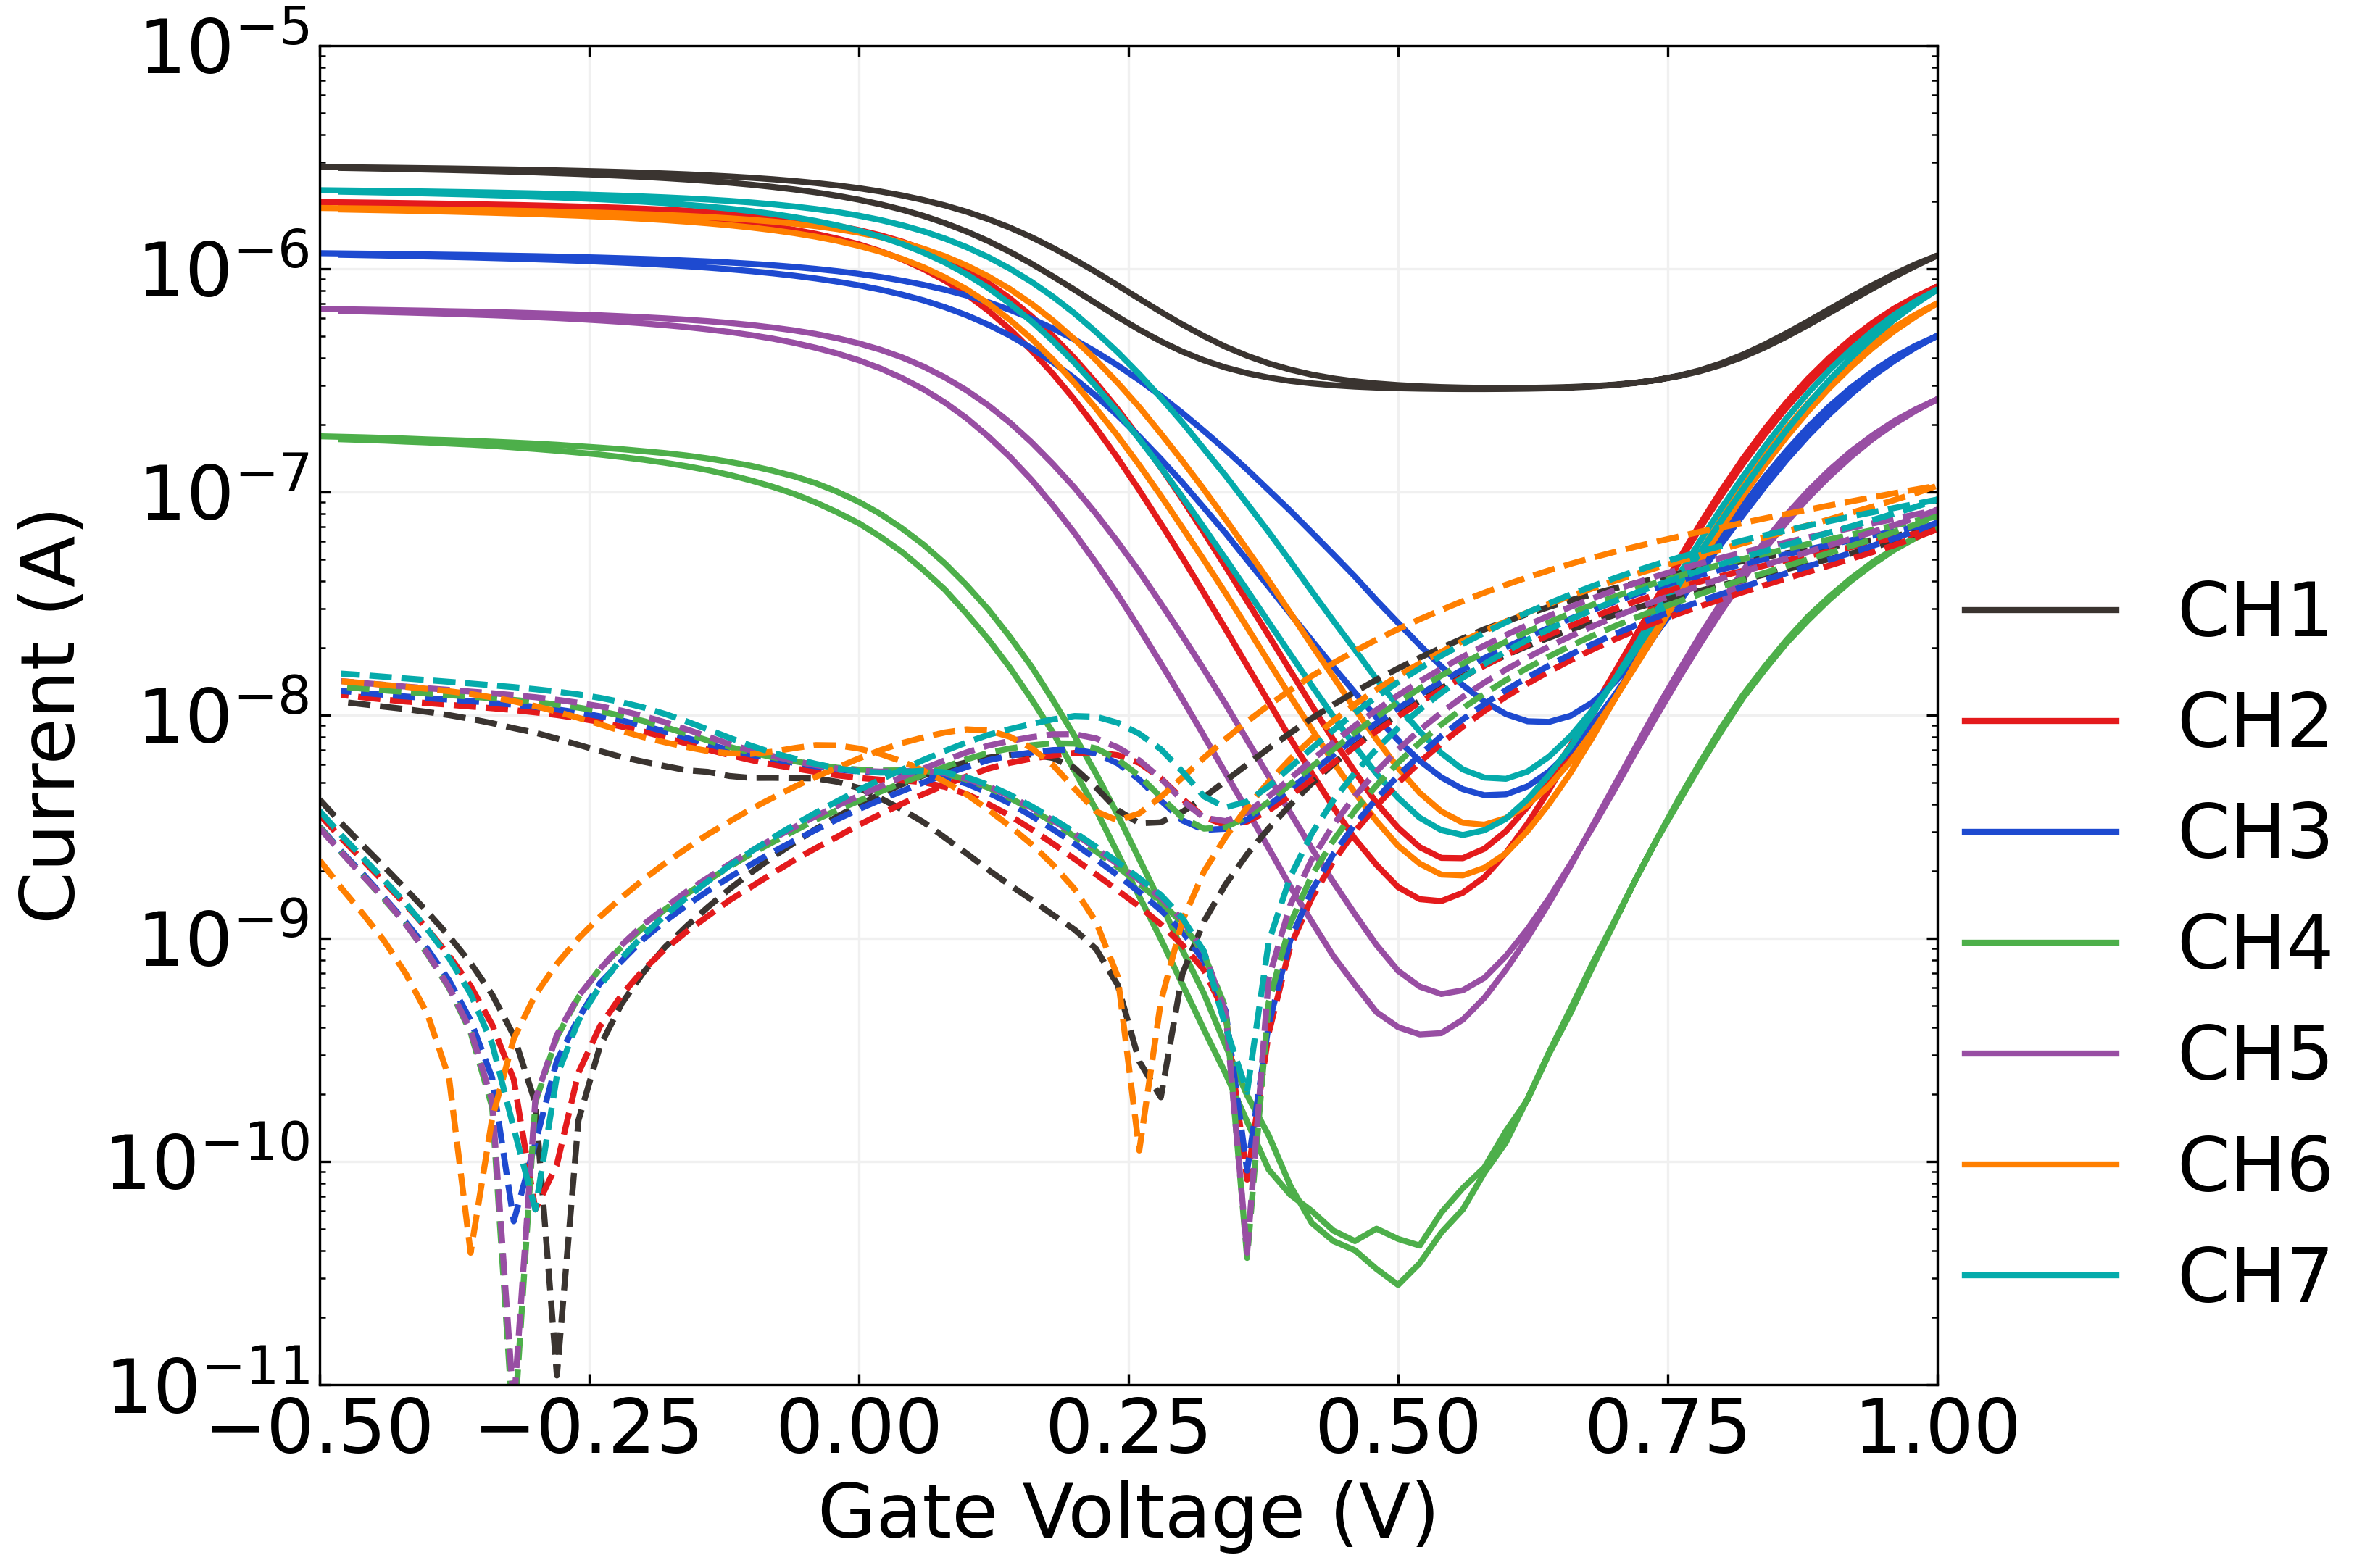
\includegraphics{figures/ch5/NTQ24C8_pristine_TXLG01_220211_solvent_gate.png}

}

}

\subcaption{\label{fig-solvent-tx-lg}Solvent-based deposition,
liquid-gated}
\end{minipage}%
\newline
\begin{minipage}[t]{0.49\linewidth}

{\centering 

\raisebox{-\height}{

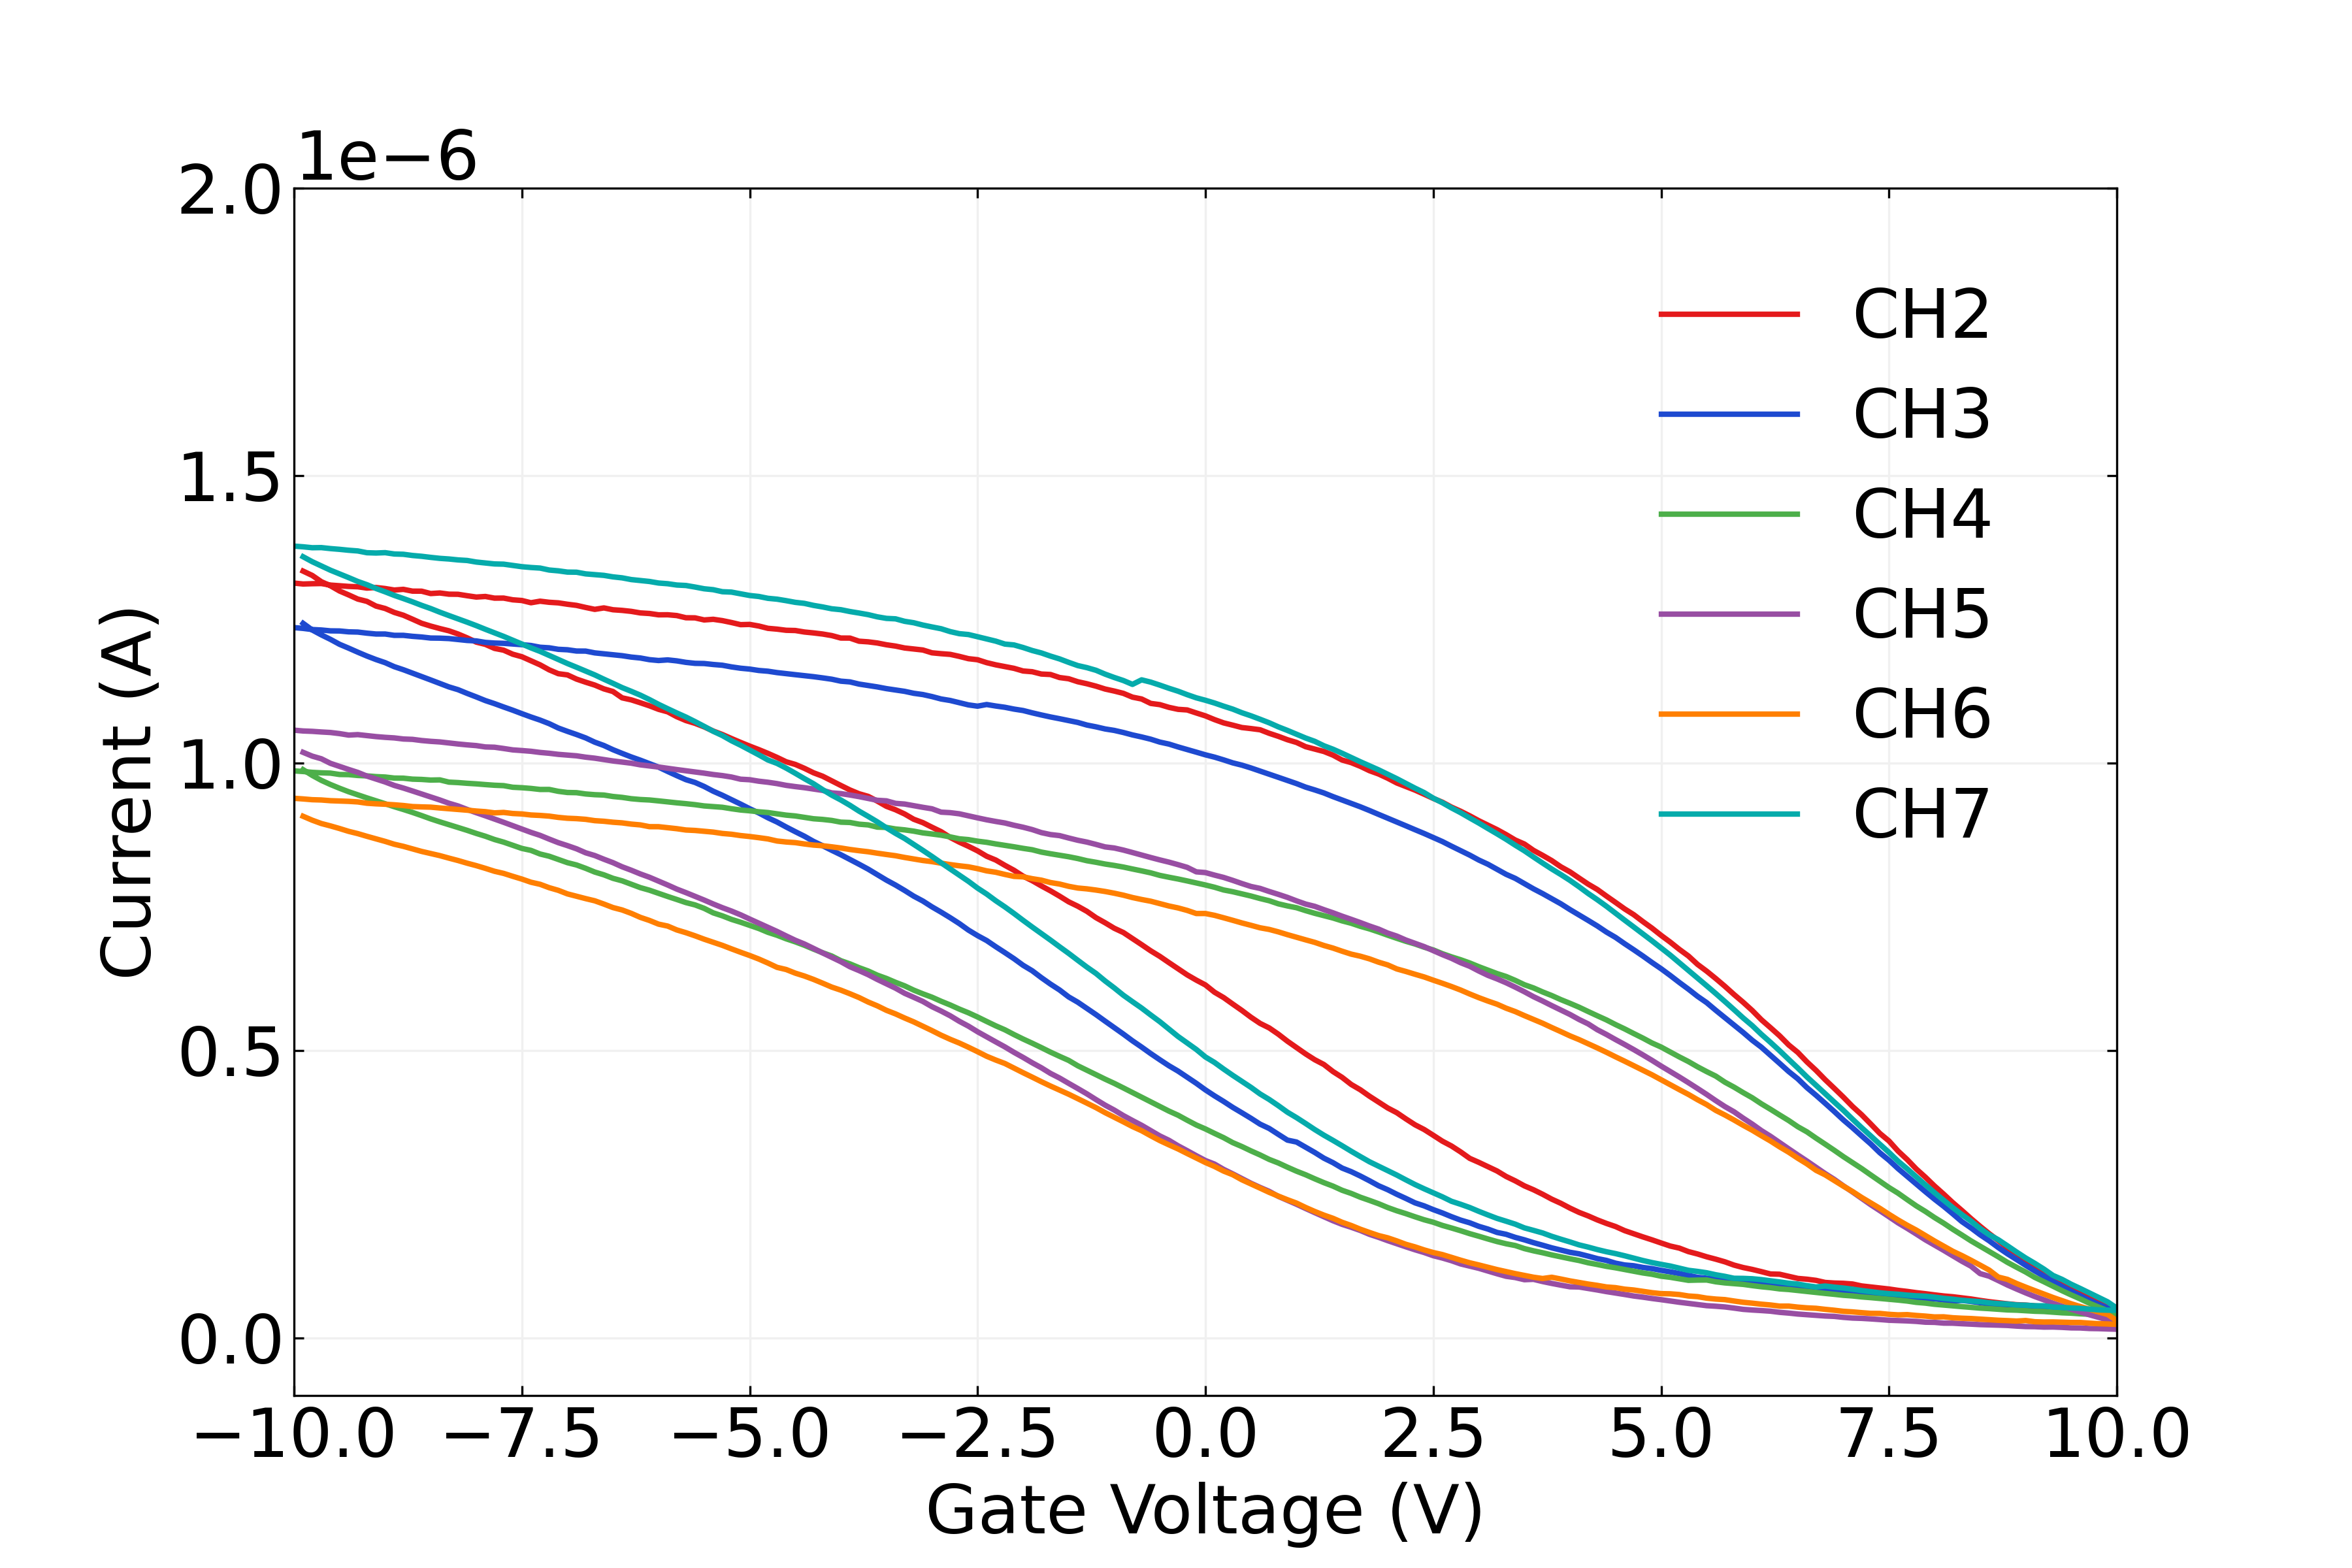
\includegraphics{figures/ch5/Q5C10_nosteam_backgate.png}

}

}

\subcaption{\label{fig-surf-tx-bg}Dropcast surfactant-based deposition,
back-gated}
\end{minipage}%
%
\begin{minipage}[t]{0.02\linewidth}

{\centering 

~

}

\end{minipage}%
%
\begin{minipage}[t]{0.49\linewidth}

{\centering 

\raisebox{-\height}{

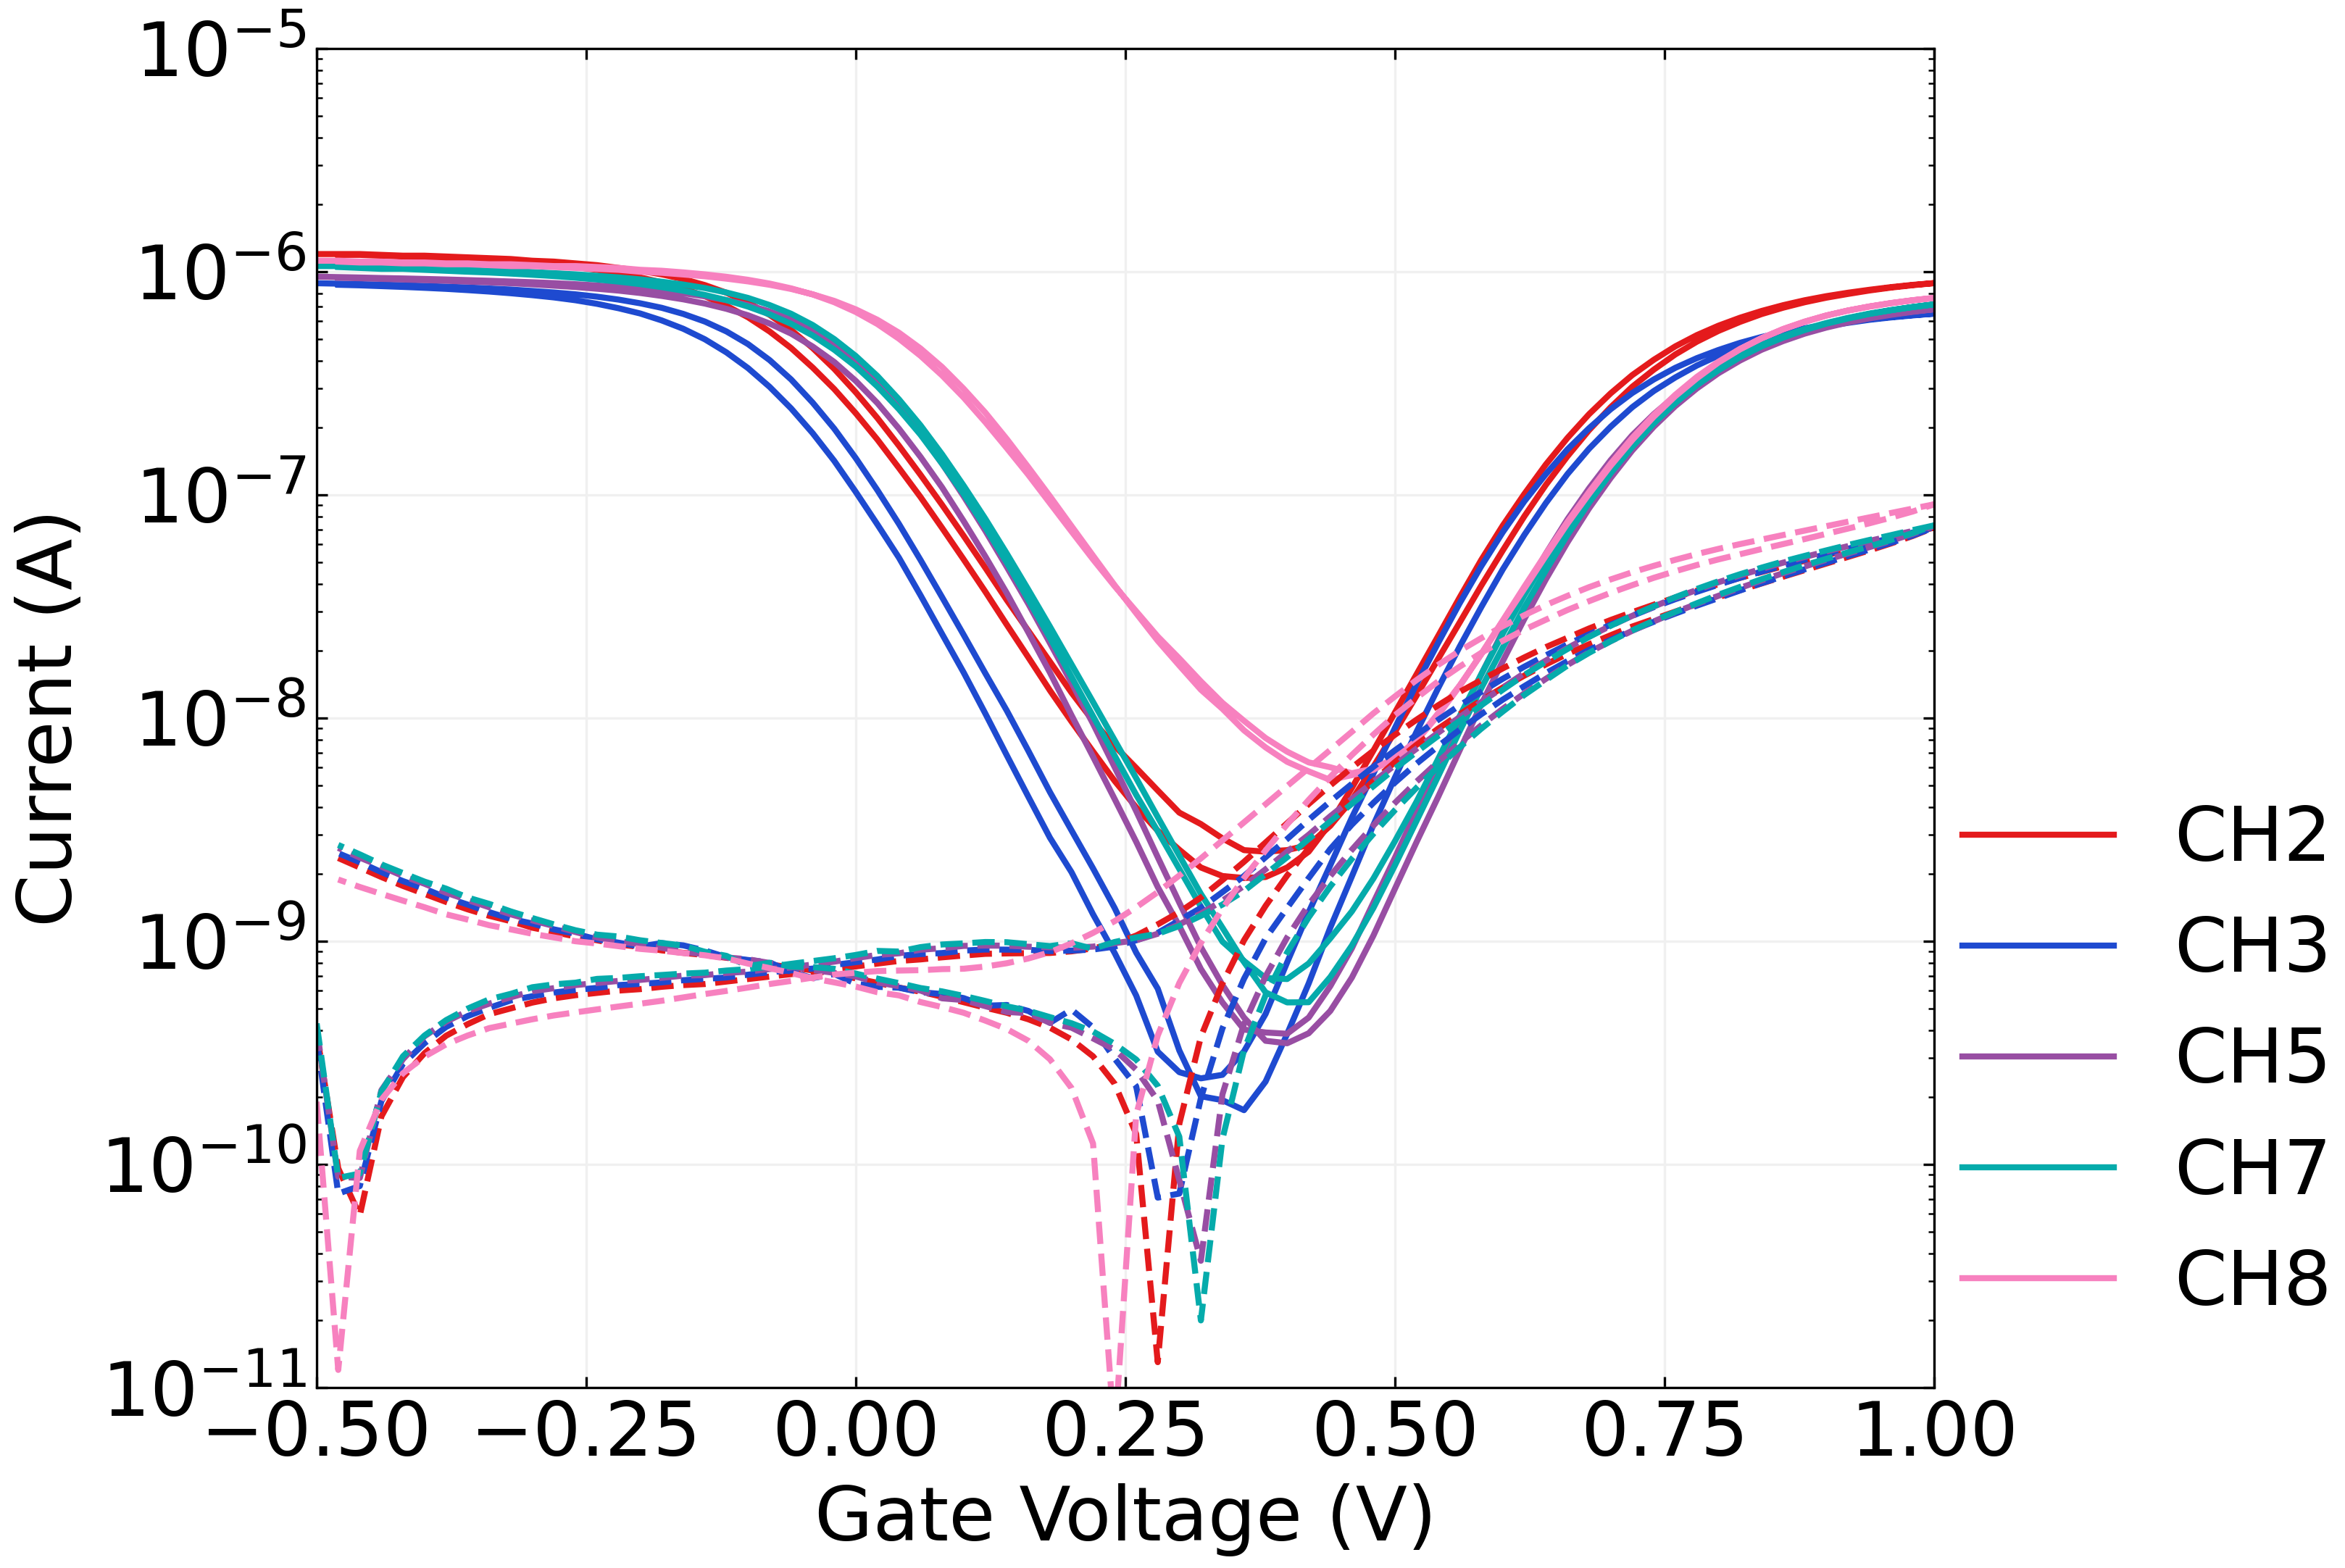
\includegraphics{figures/ch5/NTQ5C3_pristine_TXLG01_210602_nosteam_gate.png}

}

}

\subcaption{\label{fig-surf-tx-lg}Dropcast surfactant-based deposition,
liquid-gated}
\end{minipage}%
\newline
\begin{minipage}[t]{0.49\linewidth}

{\centering 

\raisebox{-\height}{

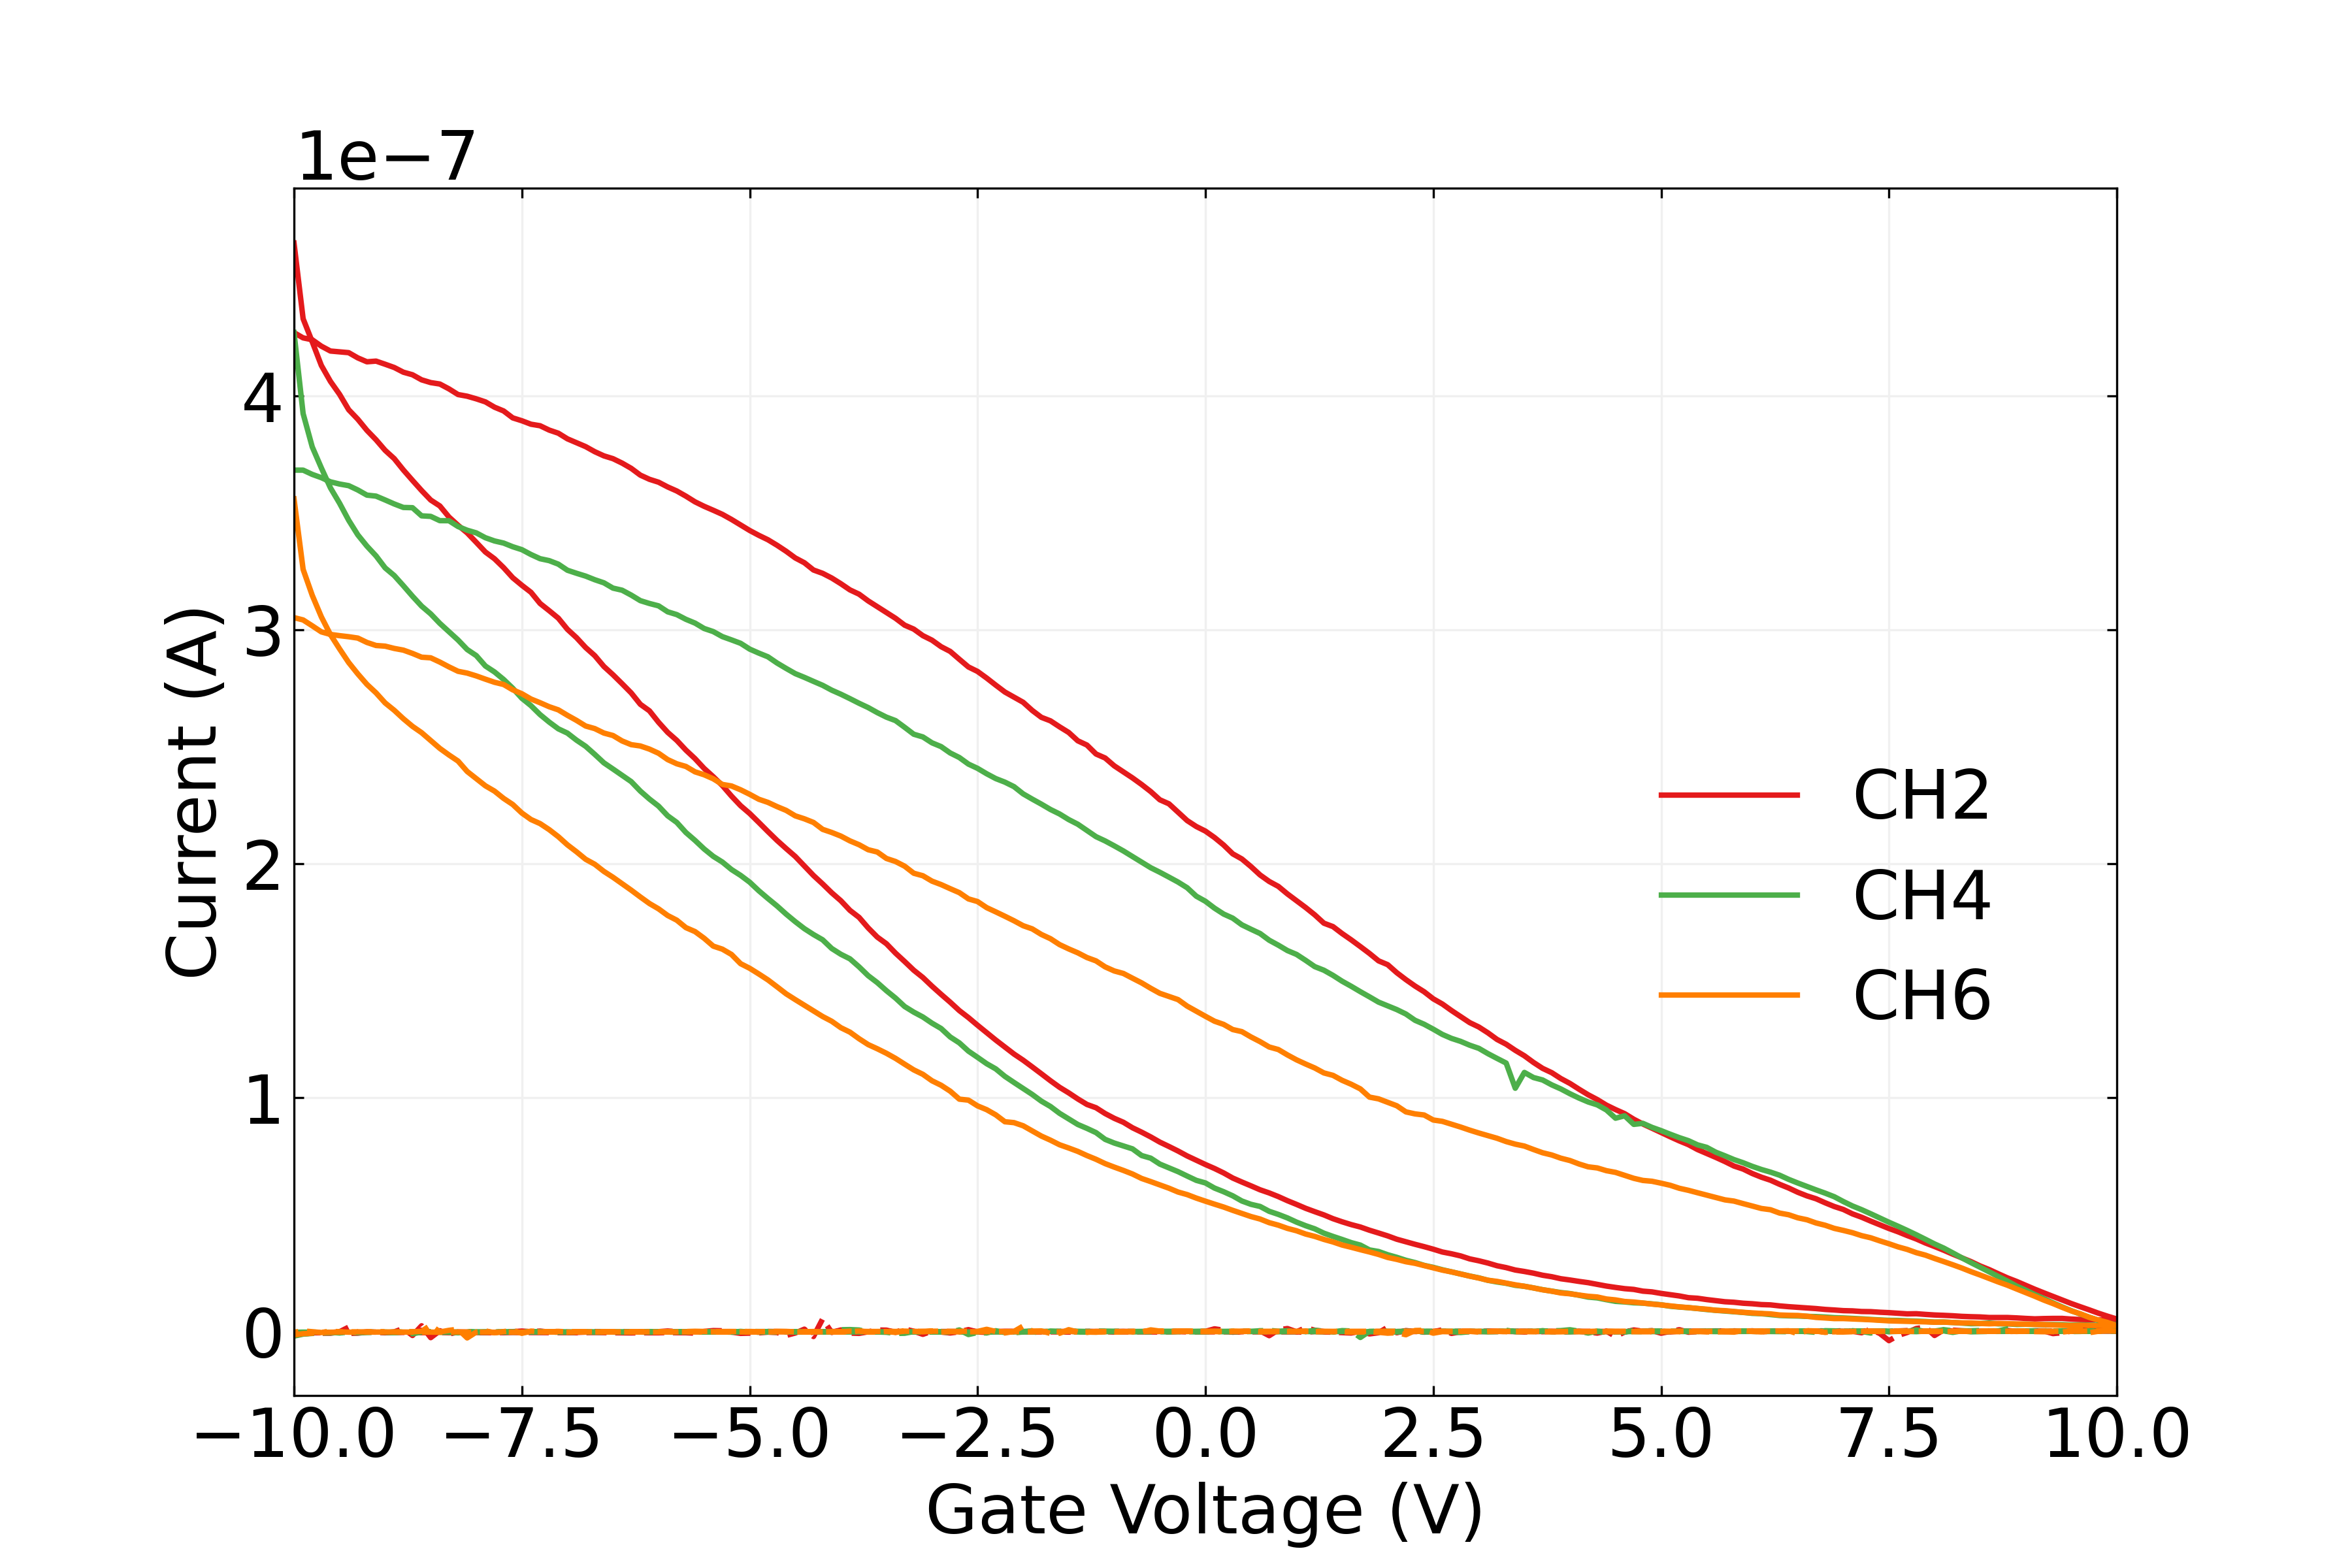
\includegraphics{figures/ch5/Q18C6_steam_backgate.png}

}

}

\subcaption{\label{fig-steam-tx-bg}Steam-assisted dropcast
surfactant-based deposition, back-gated}
\end{minipage}%
%
\begin{minipage}[t]{0.02\linewidth}

{\centering 

~

}

\end{minipage}%
%
\begin{minipage}[t]{0.49\linewidth}

{\centering 

\raisebox{-\height}{

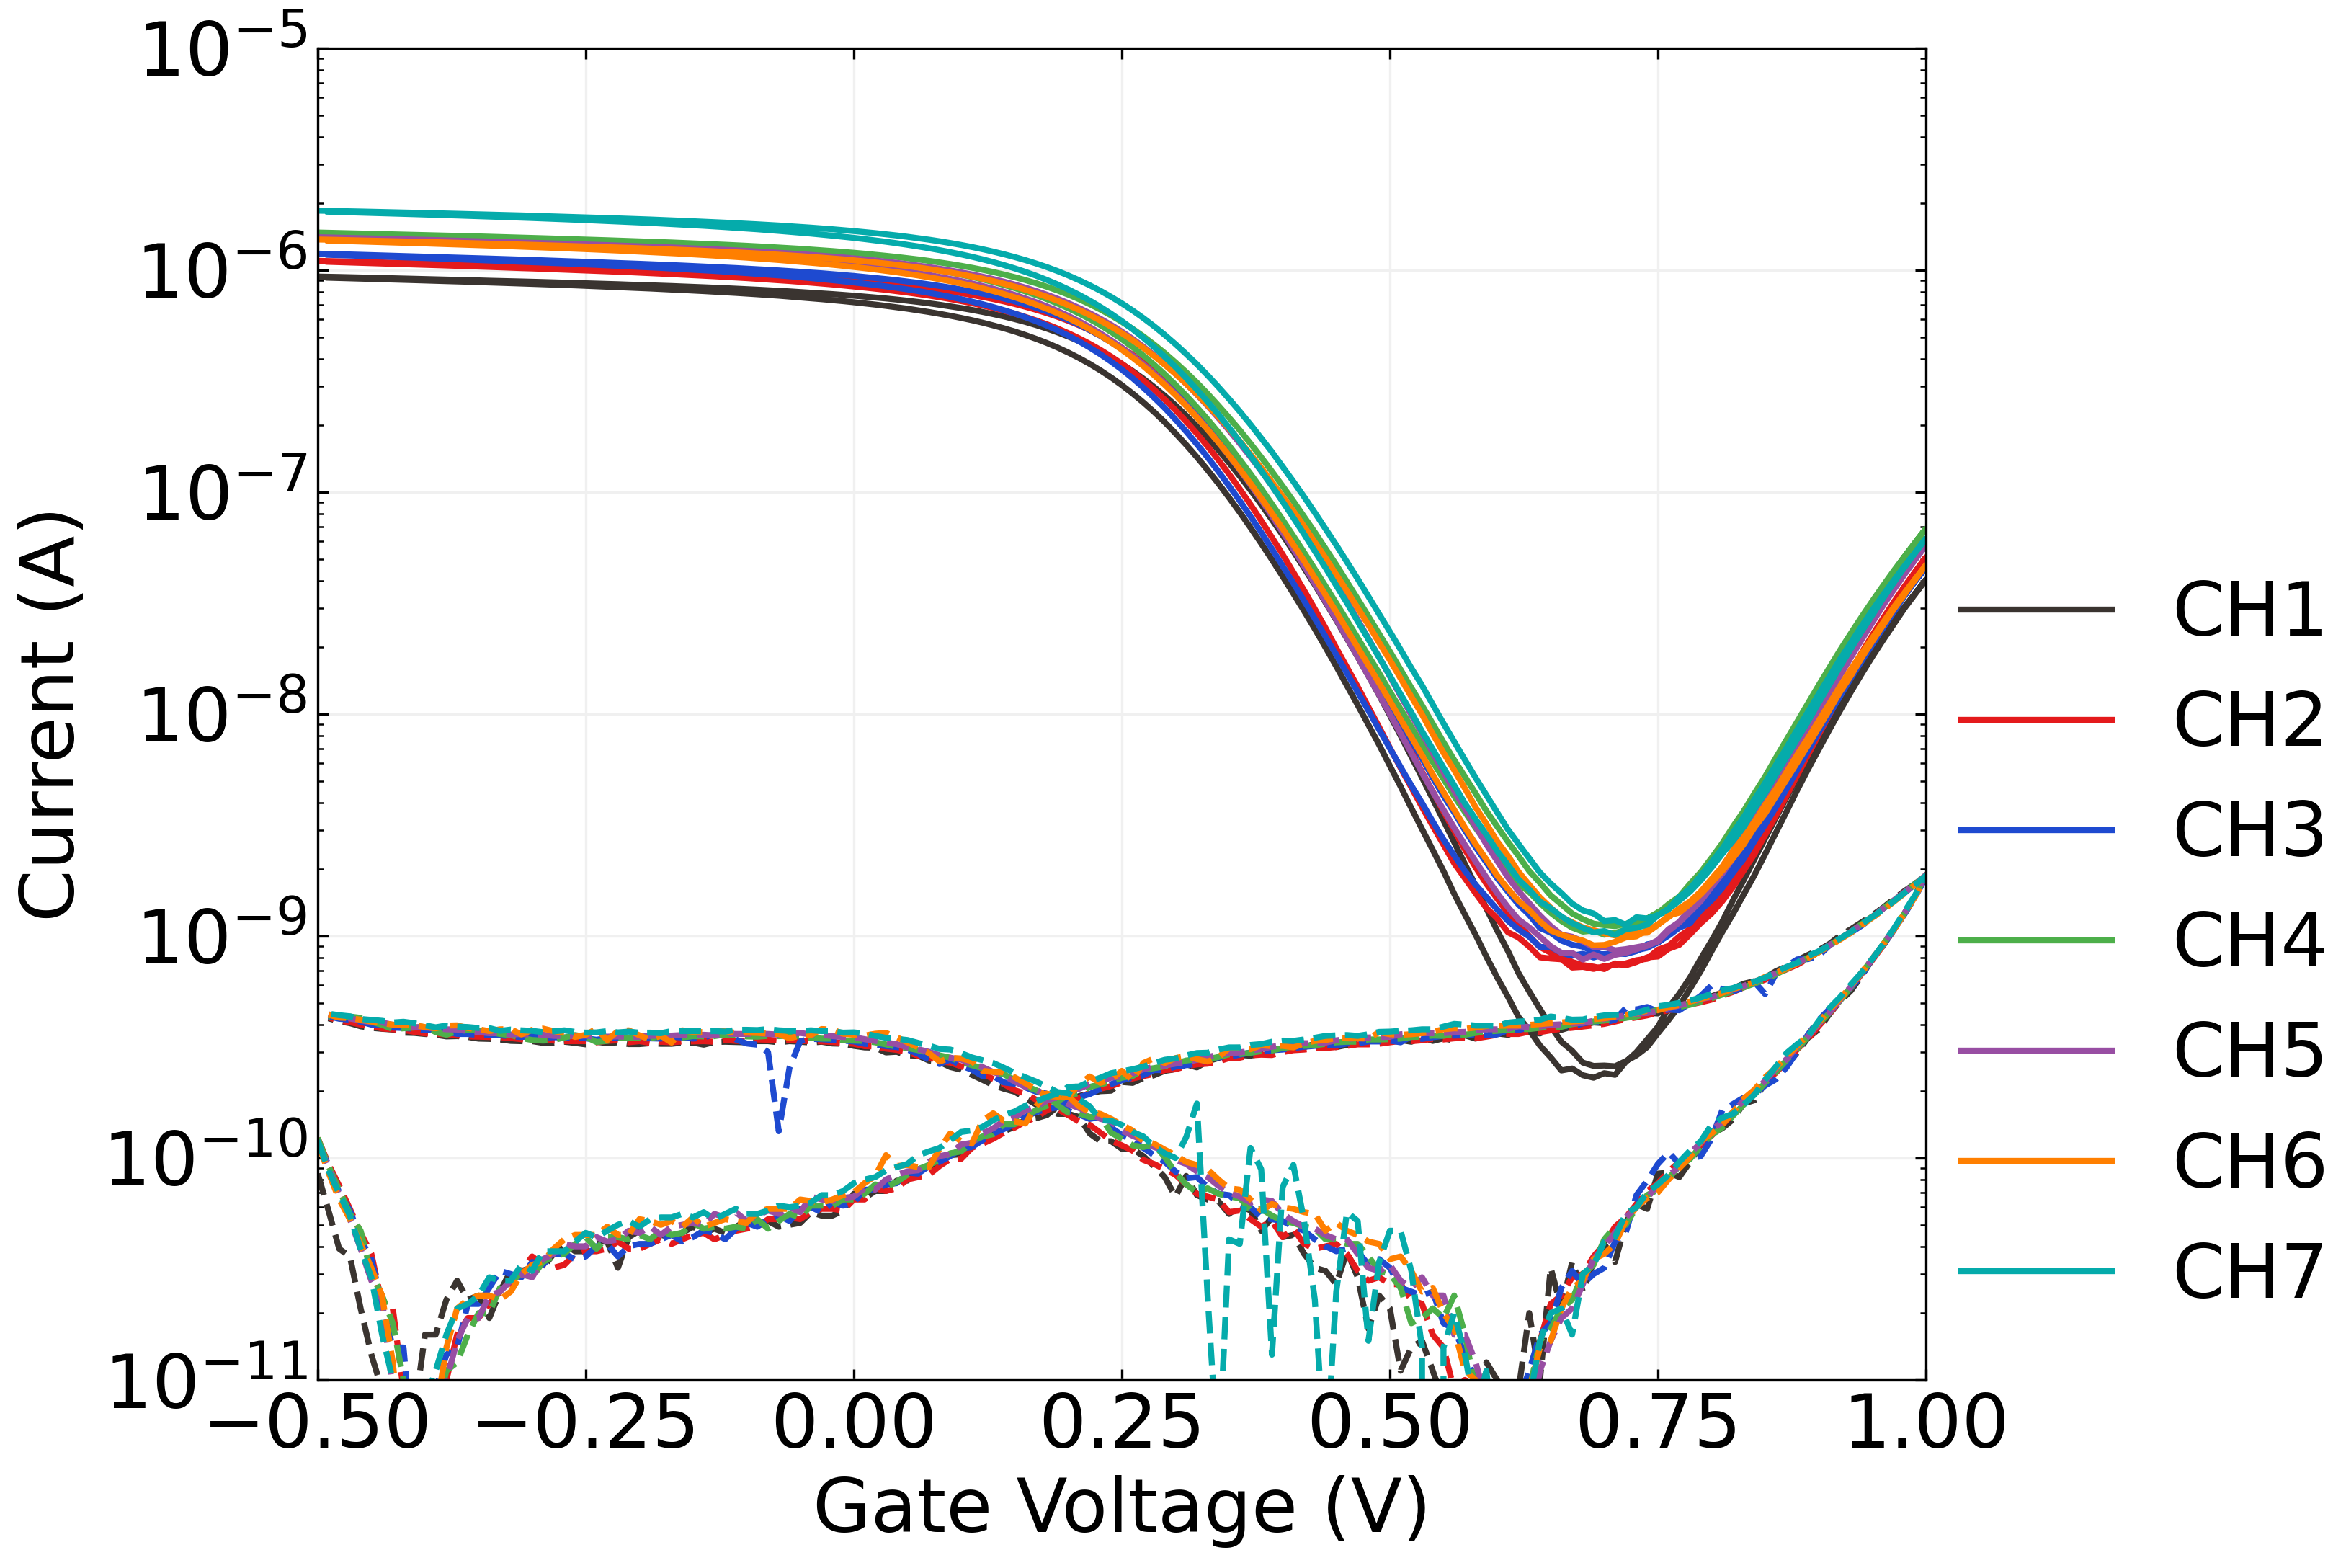
\includegraphics{figures/ch5/NTQ31C6_pristine_TXLG01_230330_steam_gate.png}

}

}

\subcaption{\label{fig-steam-tx-lg}Steam-assisted dropcast
surfactant-based deposition, liquid-gated}
\end{minipage}%

\caption{\label{fig-pristine-cnt-characteristics}Transfer
characteristics of AZ\(^\circledR\) 1518 encapsulated field-effect
transistors with carbon nanotube network channels deposited using
various methods. 1XPBS was used as the buffer for the liquid-gated
measurements here. The source-drain voltage used for all sweeps was
\(V_{ds} = 100 \textrm{mV}\). A step size of 20 mV was used for the
liquid-gated sweeps, while a step size of 100 mV was used for the
backgated sweeps. Each pair of sweeps was taken from a separate device.
Devices with a 100 nm SiO\(_2\) layer were used for backgated
measurements, and devices with a 300 nm SiO\(_2\) layer were used for
liquid gated measurements.}

\end{figure}

Each carbon nanotube device fabricated was electrically characterised as
described in \textbf{?@sec-electrical-characterisation}, and electrical
data was analysed using the Python code discussed in
Section~\ref{sec-field-effect-transistor-analysis}.

Figure~\ref{fig-pristine-cnt-characteristics} displays multi-channel
measurements of representative devices fabricated as described in
\textbf{?@sec-fabrication}. To ensure a consistent comparison, each
device here was encapsulated with AZ\(^\circledR\) 1518 encapsulation
before measurements were taken. The channels which did not exhibit
reliable transistor characteristics are not shown. These `non-working'
channels were either shorted, due to metal remaining on the channel
after lift-off, or were very low current, due to a very sparse carbon
nanotube network. Devices shown here with a solvent-deposited carbon
nanotube network were fabricated prior to Jan 2022; devices with a
surfactant-deposited network without steam present were fabricated prior
to Jun 2021; devices with a surfactant-deposited network without steam
were fabricated prior to Sep 2022.

When backgated, devices exhibited \emph{p}-type transistor behaviour
with significant hysteresis and negligible gate current leakage. The
presence of hysteresis can be explained by the presence of defects or
charge traps within and on the surface of the silicon dioxide and at
interfaces between the silicon dioxide and carbon nanotubes
\autocite{Lee2007,Lee2012,Ha2014}. The devices fabricated with a
solvent-based deposition were switched off at a lower voltage than the
devices which used surfactant during deposition.

\begin{figure}

\begin{minipage}[t]{0.47\linewidth}

{\centering 

\raisebox{-\height}{

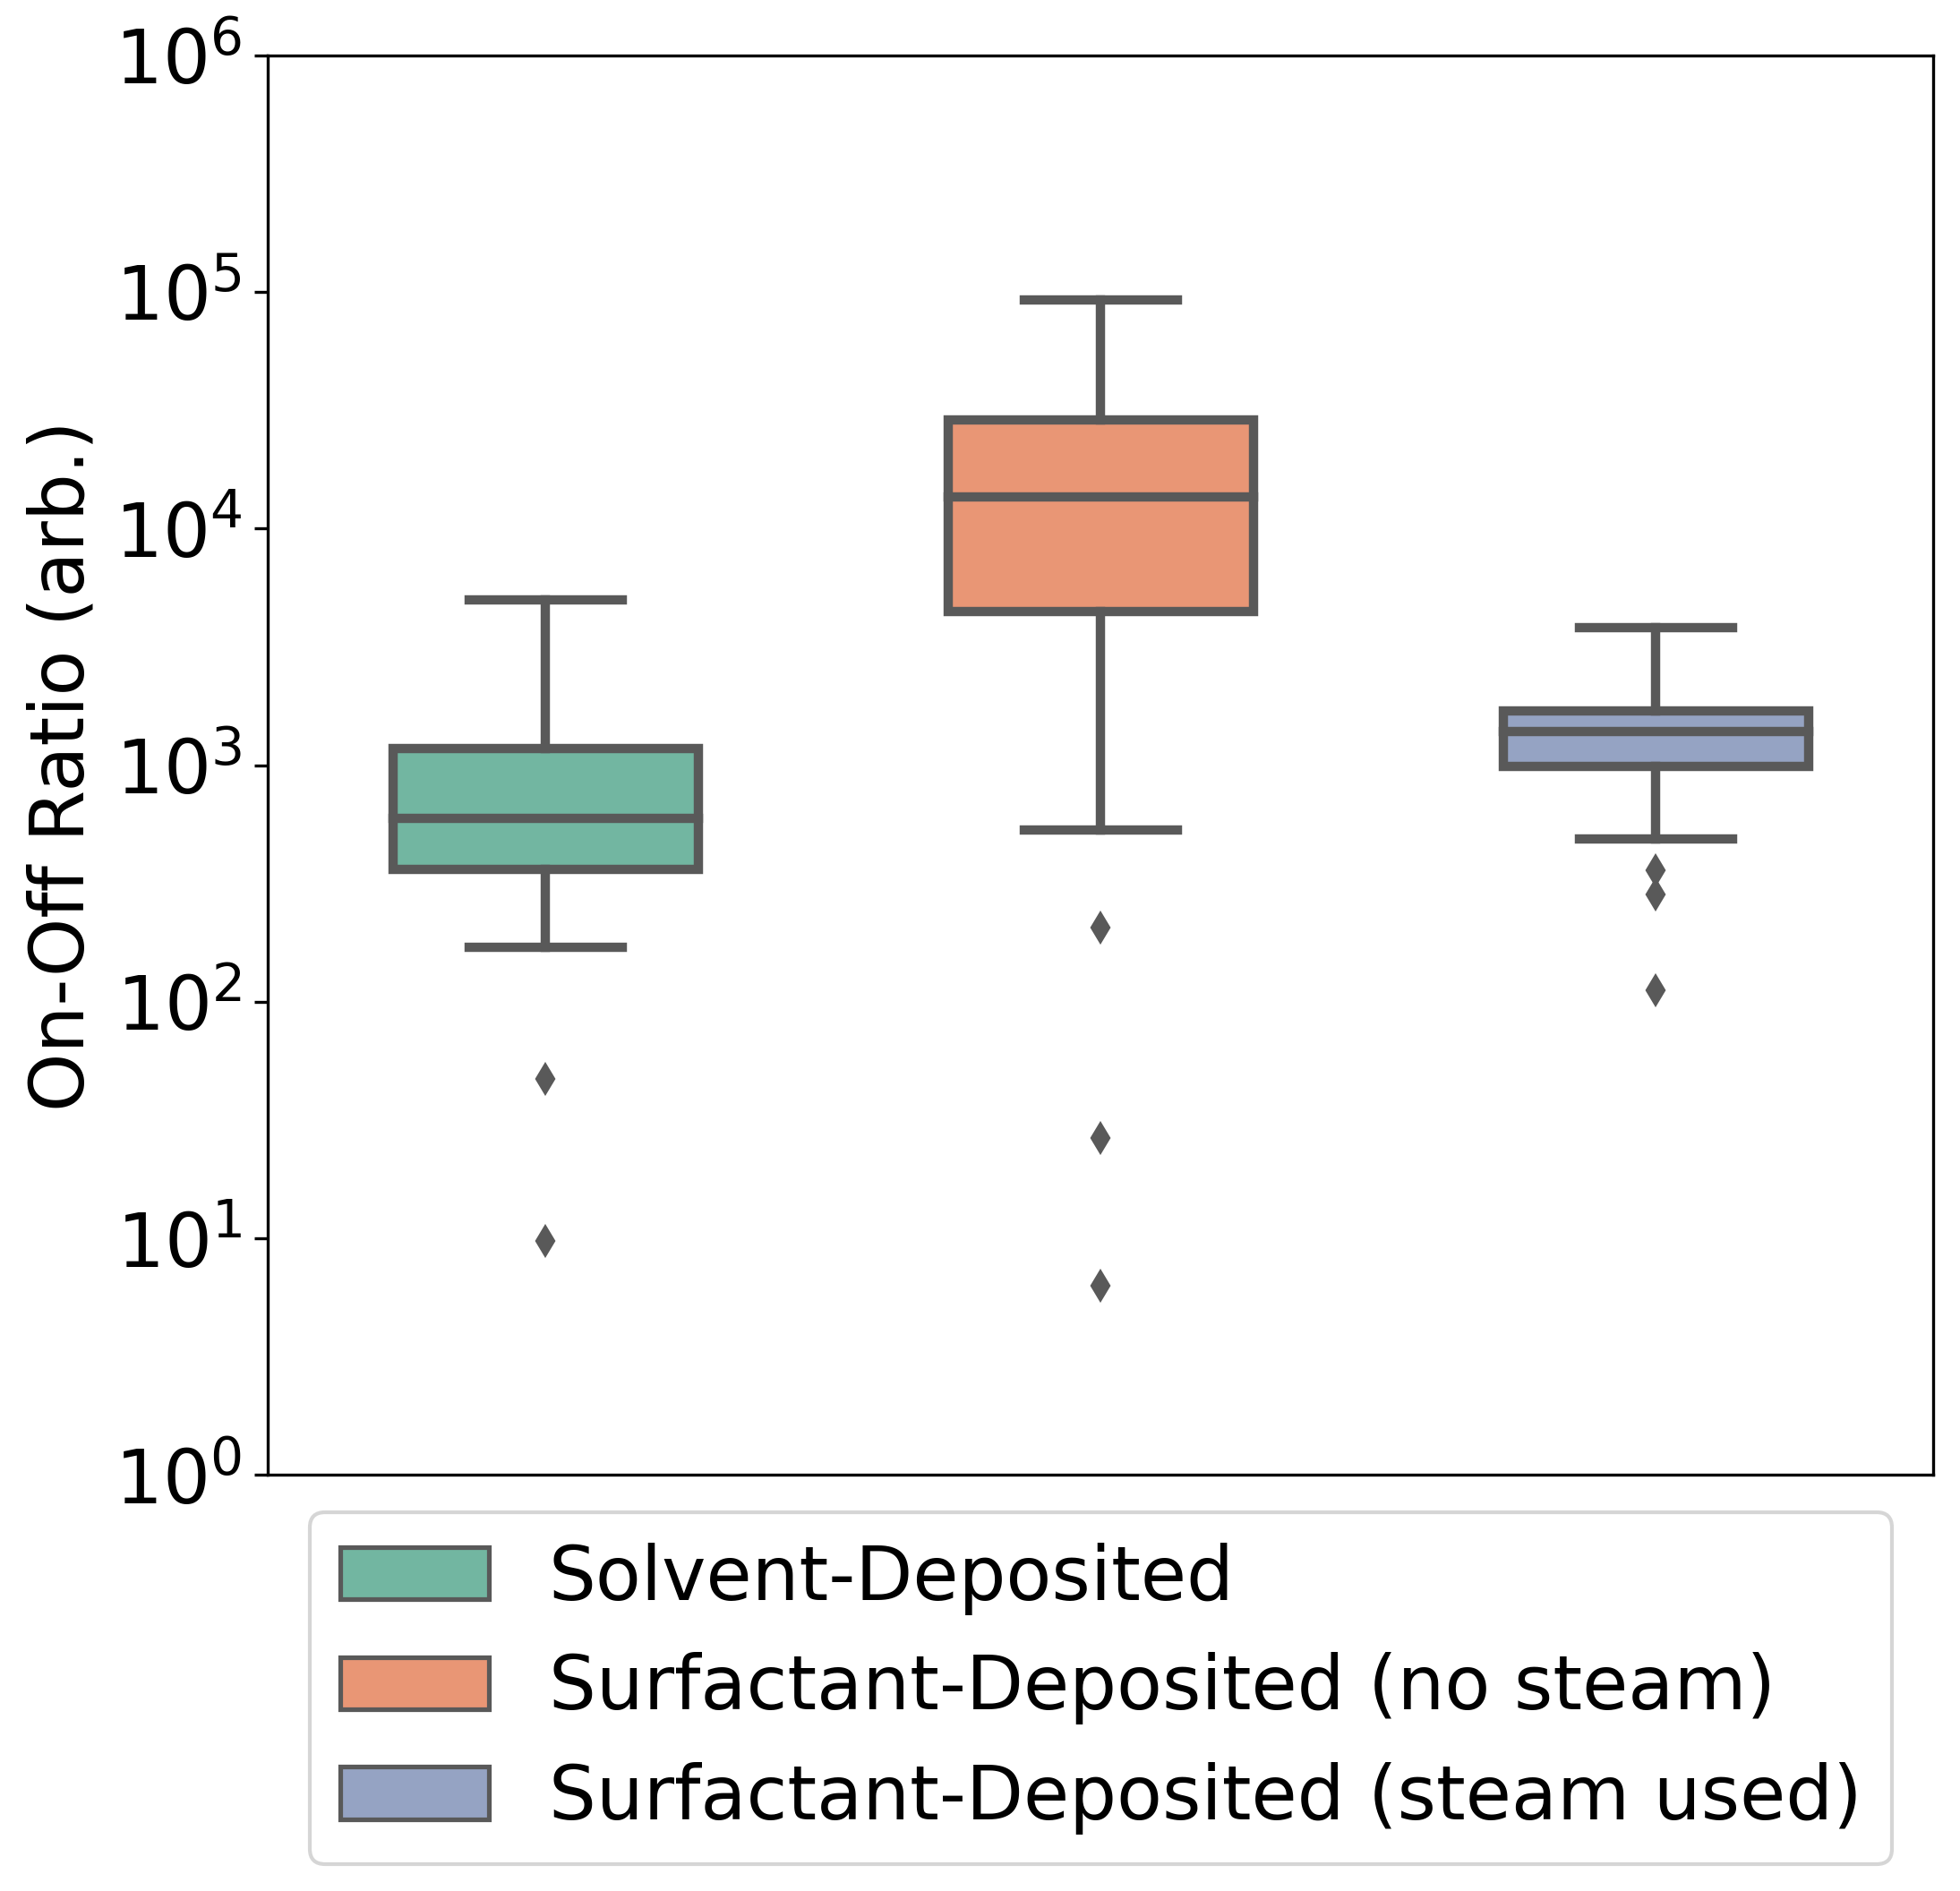
\includegraphics{figures/ch5/onoff_CNT.png}

}

}

\subcaption{\label{fig-on-off-ratio}}
\end{minipage}%
%
\begin{minipage}[t]{0.05\linewidth}

{\centering 

~

}

\end{minipage}%
%
\begin{minipage}[t]{0.47\linewidth}

{\centering 

\raisebox{-\height}{

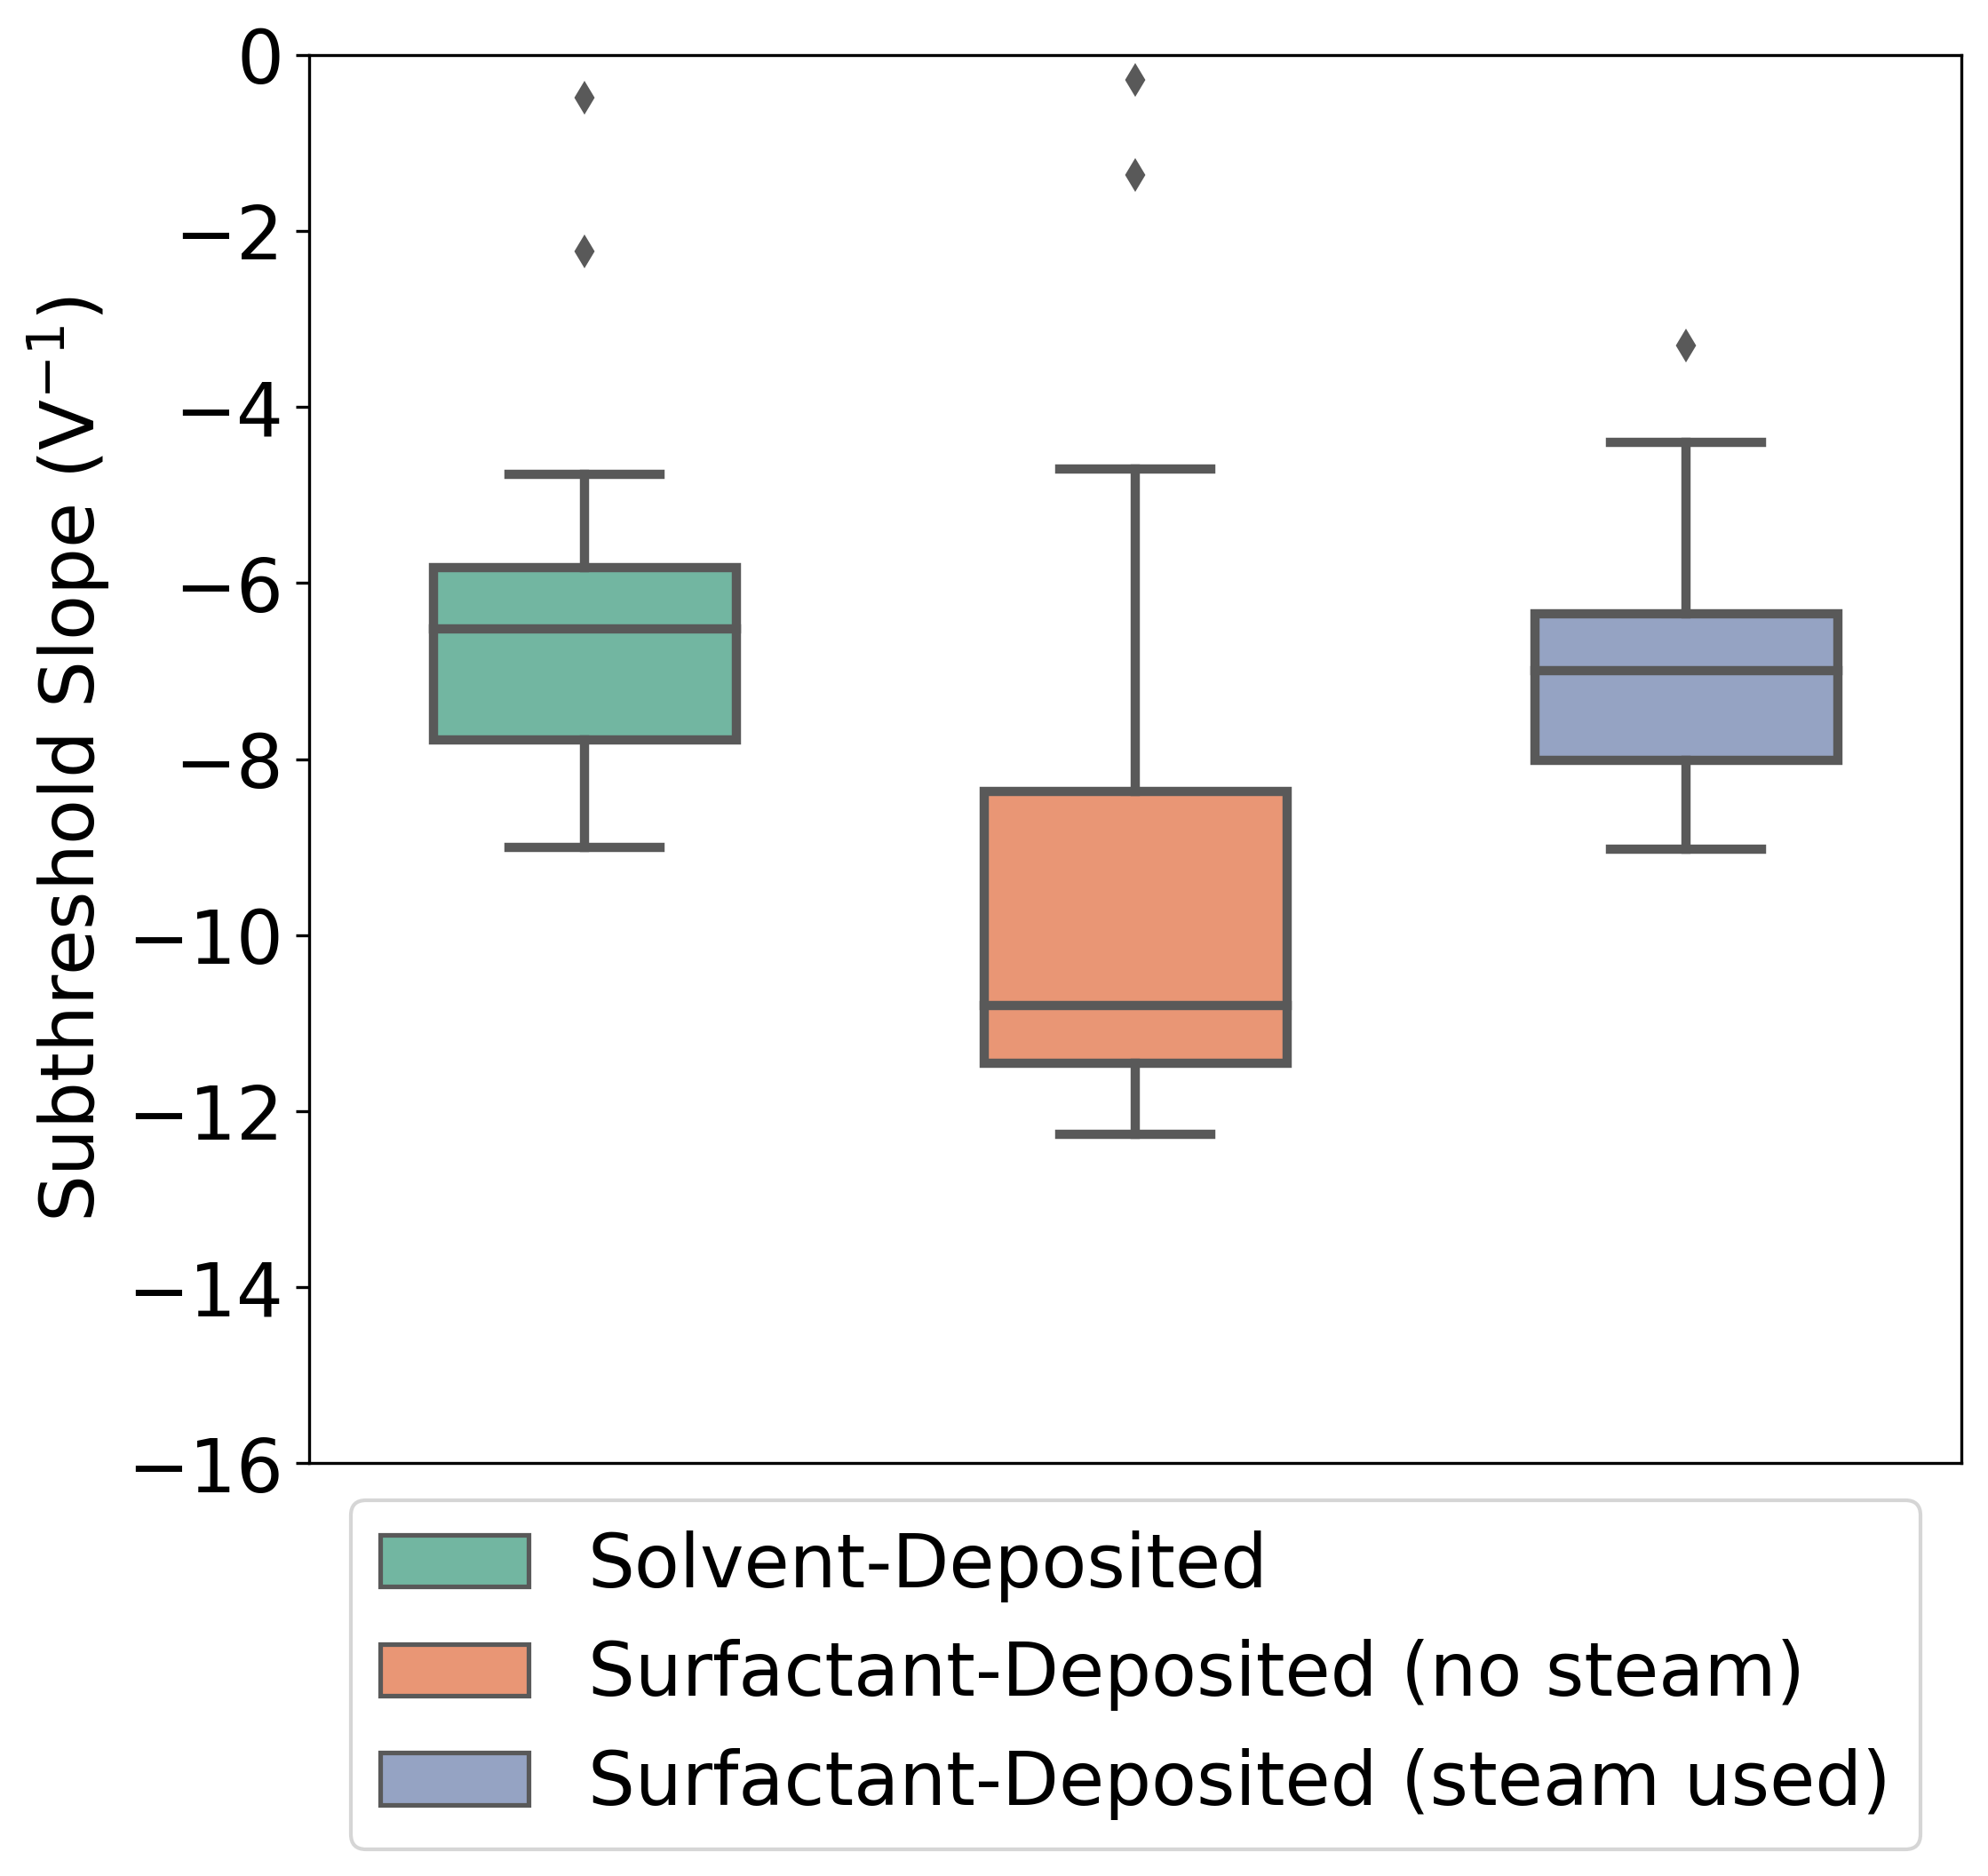
\includegraphics{figures/ch5/SS.png}

}

}

\subcaption{\label{fig-subthreshold-slope}}
\end{minipage}%
\newline
\begin{minipage}[t]{0.26\linewidth}

{\centering 

~

}

\end{minipage}%
%
\begin{minipage}[t]{0.47\linewidth}

{\centering 

\raisebox{-\height}{

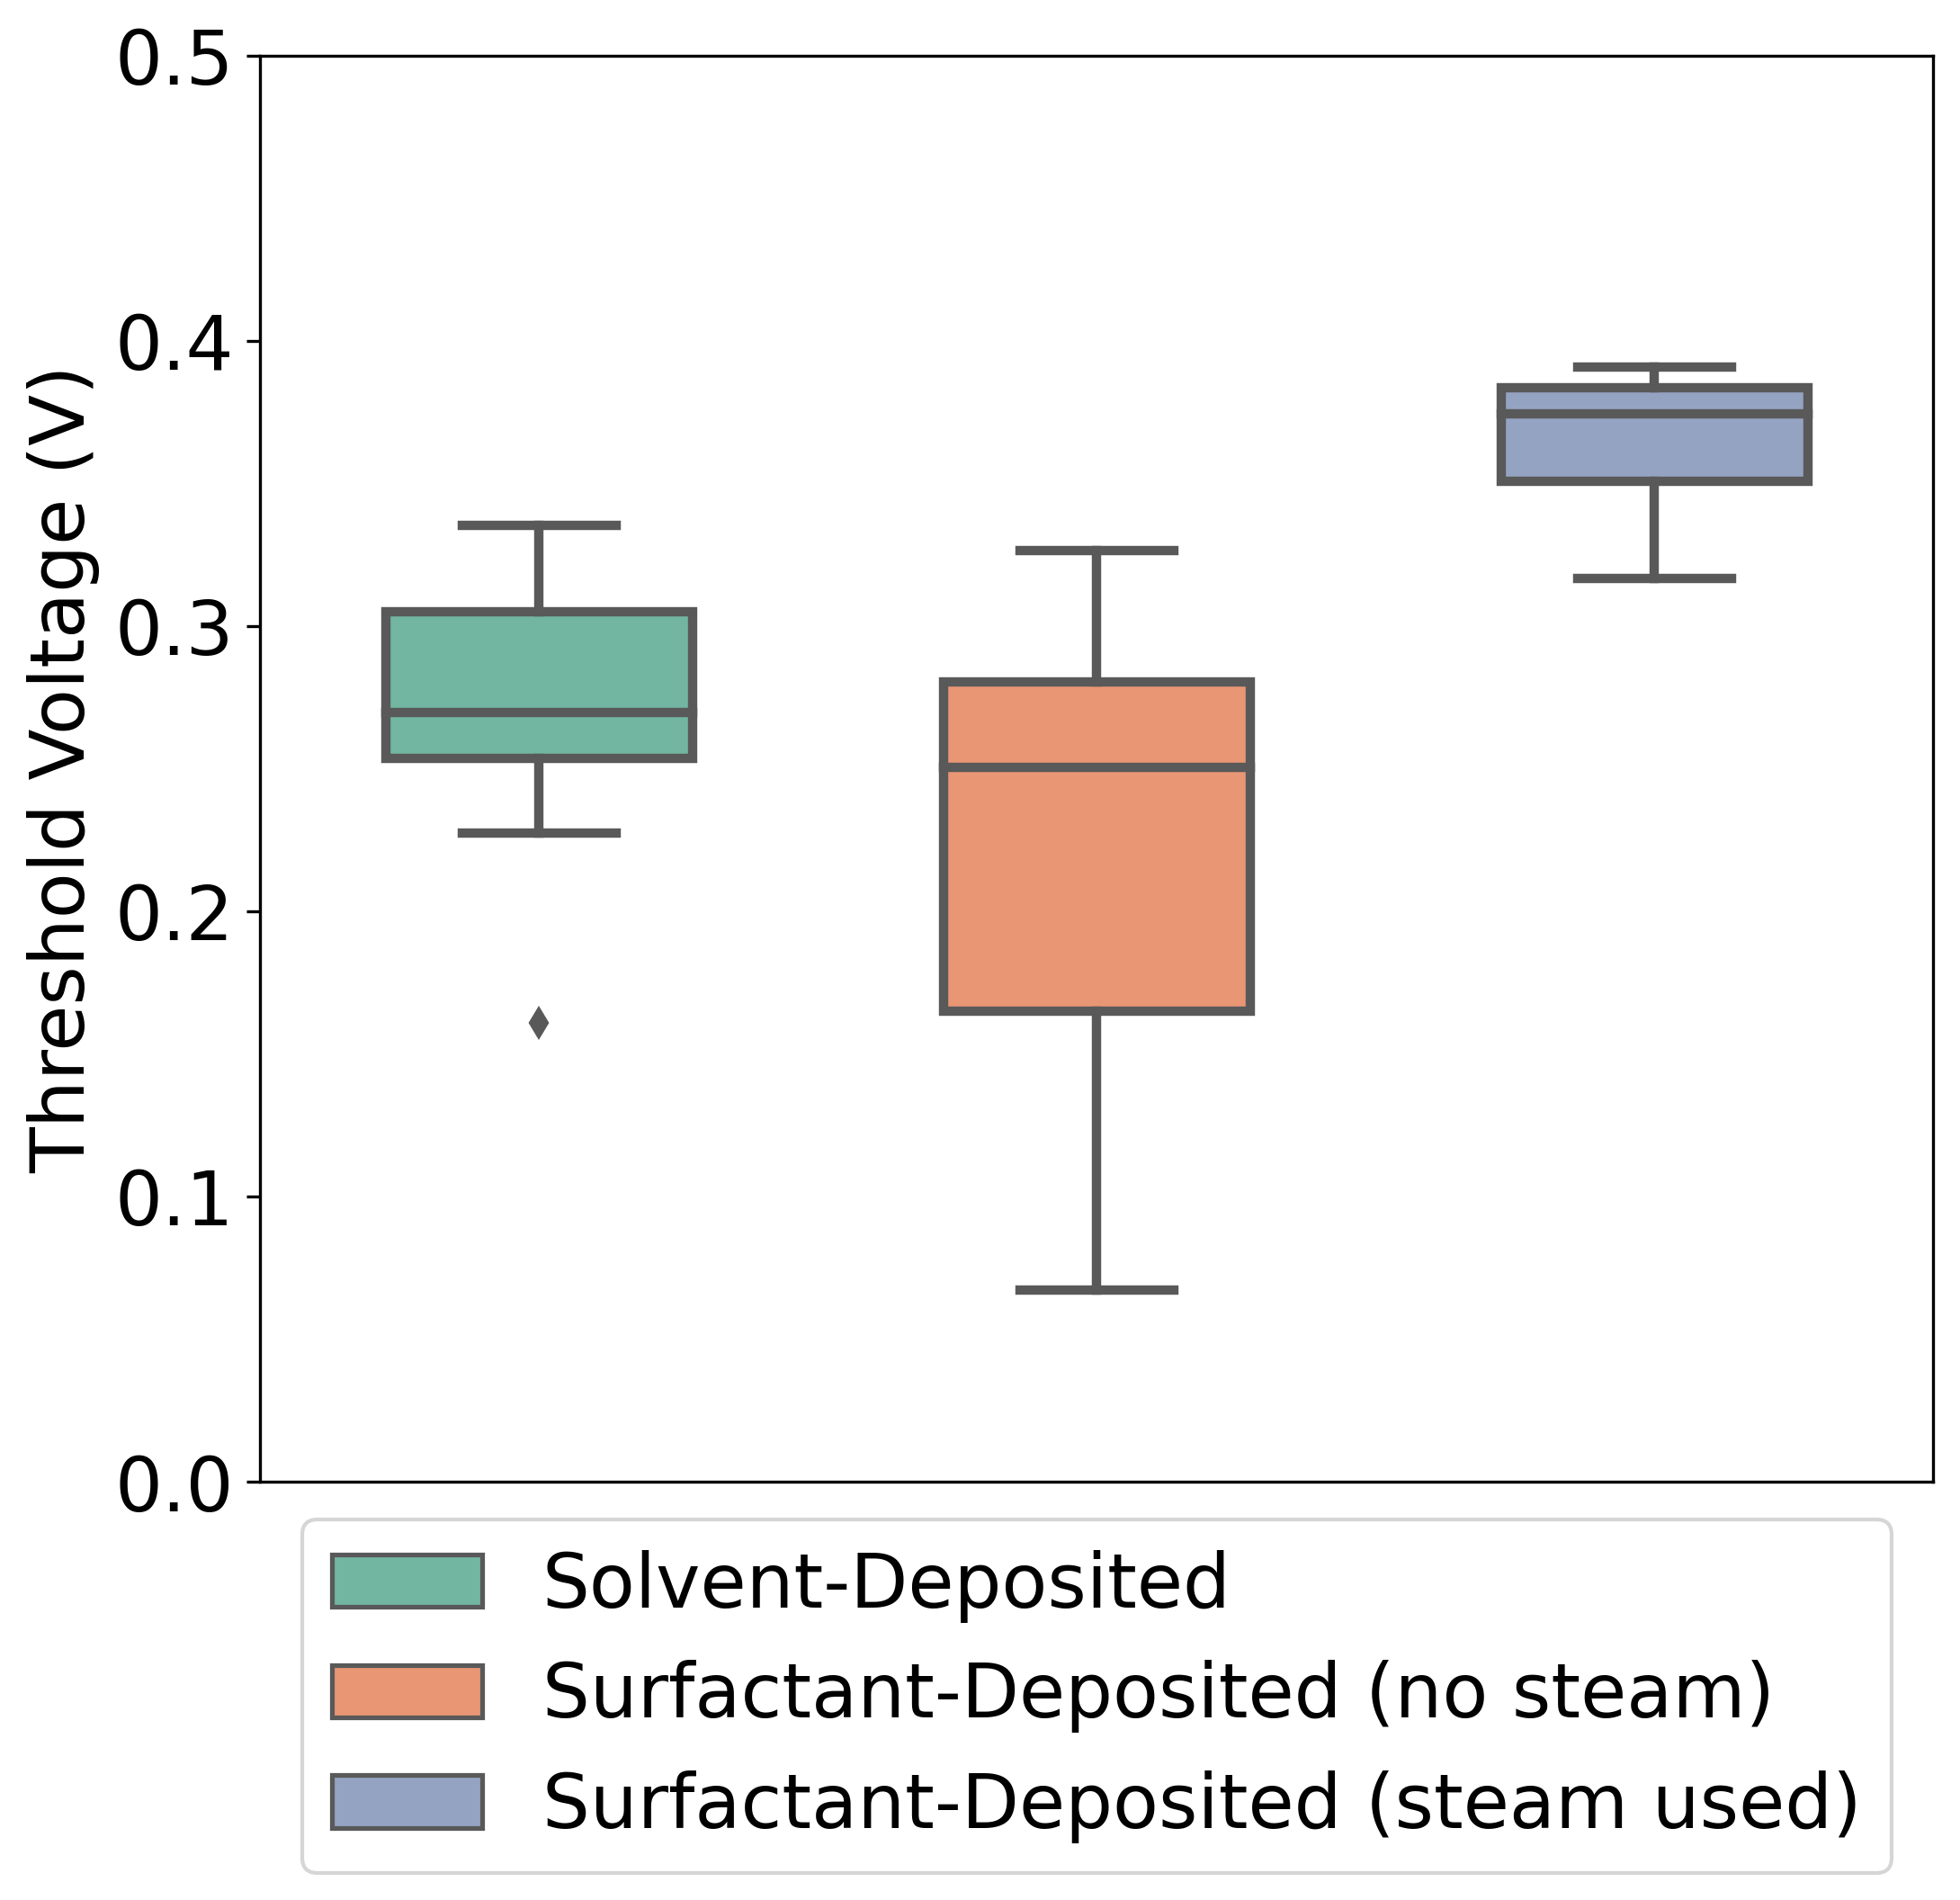
\includegraphics{figures/ch5/threshold_V.png}

}

}

\subcaption{\label{fig-threshold-voltage}}
\end{minipage}%
%
\begin{minipage}[t]{0.26\linewidth}

{\centering 

~

}

\end{minipage}%

\caption{\label{fig-sweep-parameters}These boxplots illustrate the
statistical distribution of (a) the on-off ratio, (b) the subthreshold
slope, and (c) the threshold voltage of AZ\(^\circledR\) 1518
encapsulated liquid-gated transistor channels corresponding to each type
of carbon nanotube film deposition. For each deposition type, electrical
characteristics were taken of 21 channels of at least three separate
devices. The boxes indicate the 25th and 75th percentile of the
distribution.}

\end{figure}

When the devices were liquid-gated with 1XPBS electrolyte, they
exhibited ambipolar characteristics, commonly observed in carbon
nanotube network FETs
\autocite{Kauffman2008,Heller2009,JongYu2009,Derenskyi2014,Murugathas2018,Albarghouthi2022}.
When devices were appropriately configured, leakage current did not
exceed \(\sim 1 \times 10^{-7}\) V across the forward and reverse sweep.
Devices generally exhibited significantly less hysteresis than in the
backgated case. The devices shown which used carbon nanotube films
deposited in surfactant with steam present showed the least hysteresis,
which is largely due to the relatively small diameter of the bundles in
these films \autocite{Pop2009}. These devices also showed significantly
less channel-to-channel variation in electrical characteristics more
generally. A summary of key parameters of pristine liquid-gated devices
is shown in Figure~\ref{fig-sweep-parameters}. The full dataset consists
of three sets of 21 liquid-gated transfer characteristics of working
channels, with each set corresponding to the use of a particular method
of carbon nanotube network deposition in the device fabrication.
Measurements from at least three devices are included in each set. Each
entry in the summary corresponds to the average of the specific
parameter in the forward and reverse sweep direction.

Channels from surfactant-deposited film devices usually showed a larger
on-off ratio and subthreshold slope than those from solvent-deposited
devices. When the transistor is gated in the subthreshold range, a
larger on-off ratio and subthreshold slope results in a larger change in
conductance in response to changes in the transfer characteristic curve.
Therefore, a larger on-off ratio and subthreshold slope is desirable for
improved sensor performance \autocite{Kauffman2008,Heller2009,Gao2010}.
The larger on-off ratio for surfactant-deposited film devices is likely
a result of the reduced bundling of nanotubes, as discussed in
Section~\ref{sec-pristine-morphology}. Carbon nanotube pathways across
the channel with a lower degree of bundling will have a lower number of
component metallic tubes in the network, which increases the on-off
ratio \autocite{LeMieux2008,Rouhi2011,Murugathas2018}. The effect of
metallic nanotubes increasing the off current of a device channel is
illustrated by channel 1 in Figure~\ref{fig-solvent-tx-lg}. The larger
subthreshold slope is likely due to increased mobility from a denser
nanotube network in surfactant-deposited films \autocite{Rouhi2011}, as
seen in Figure~\ref{fig-afm-morphology}.

When steam is used for surfactant deposition of films, the resulting
devices showed highly consistent channel-to-channel electrical
properties. As the carbon nanotube films on these devices are relatively
dense, as seen in Figure~\ref{fig-afm-morphology}, we know that the
network is well above the percolation threshold. As many carbon nanotube
pathways connect across the channel in parallel, small variations in the
network morphology have less of an impact on the overall channel
behaviour \autocite{Murugathas2018}. We also see from
Table~\ref{tbl-histogram-parameters} that the range of bundle sizes is
relatively low in the steam-deposited films used in these devices. The
low range of bundle sizes means the semiconducting-metallic nanotube
ratio is far more consistent for these devices, leading to more
consistent electrical device characteristics. Being able to achieve
consistent subthreshold regime behaviour between channels on the same
device is a desirable attribute for reliable real-time multiplexed
biosensing \autocite{Kauffman2008,Heller2009,Gao2010}.

All channels characterised had a positive threshold voltage
(\(V_{th}\)). The threshold voltage was largest and most consistent for
steam-assisted surfactant-deposited films. The relatively high values of
\(V_{th}\) which correspond to channel measurements from steam-assisted
surfactant-deposited devices indicates increased \(p\)-doping of the
network relative to networks deposited via alternative processes
\autocite{Kang2005,Heller2008,Murugathas2018}. It is highly likely the
dopant is present due to the steam deposition, and may be related to the
large contamination peak for steam-deposited films seen in
Figure~\ref{fig-afm-morphology} and \textbf{?@fig-remaining-histogram}.
One possibility is that this dopant is residual surfactant, which can
\(p\)-dope carbon nanotubes as well as enhancing \(p\)-doping from
adsorped oxygen and water \autocite{Kane2014,Nonoguchi2018}. We have
seen that steam prevents bundling of carbon nanotubes during deposition.
This effect is likely due to persistence of the surfactant keeping
nanotubes separate during this process. Presence of surfactant may also
explain the lowered subthreshold slope and therefore mobility of the
surfactant-deposited devices with steam relative to the
surfactant-deposited devices without steam. The analysis by Kane
\emph{et al.} shows that the thermal annealling at 150\(^\circ\)C used
in this work to remove residual surfactant is likely inadequate for this
purpose \autocite{Kane2014}.

\begin{figure}

\begin{minipage}[t]{0.47\linewidth}

{\centering 

\raisebox{-\height}{

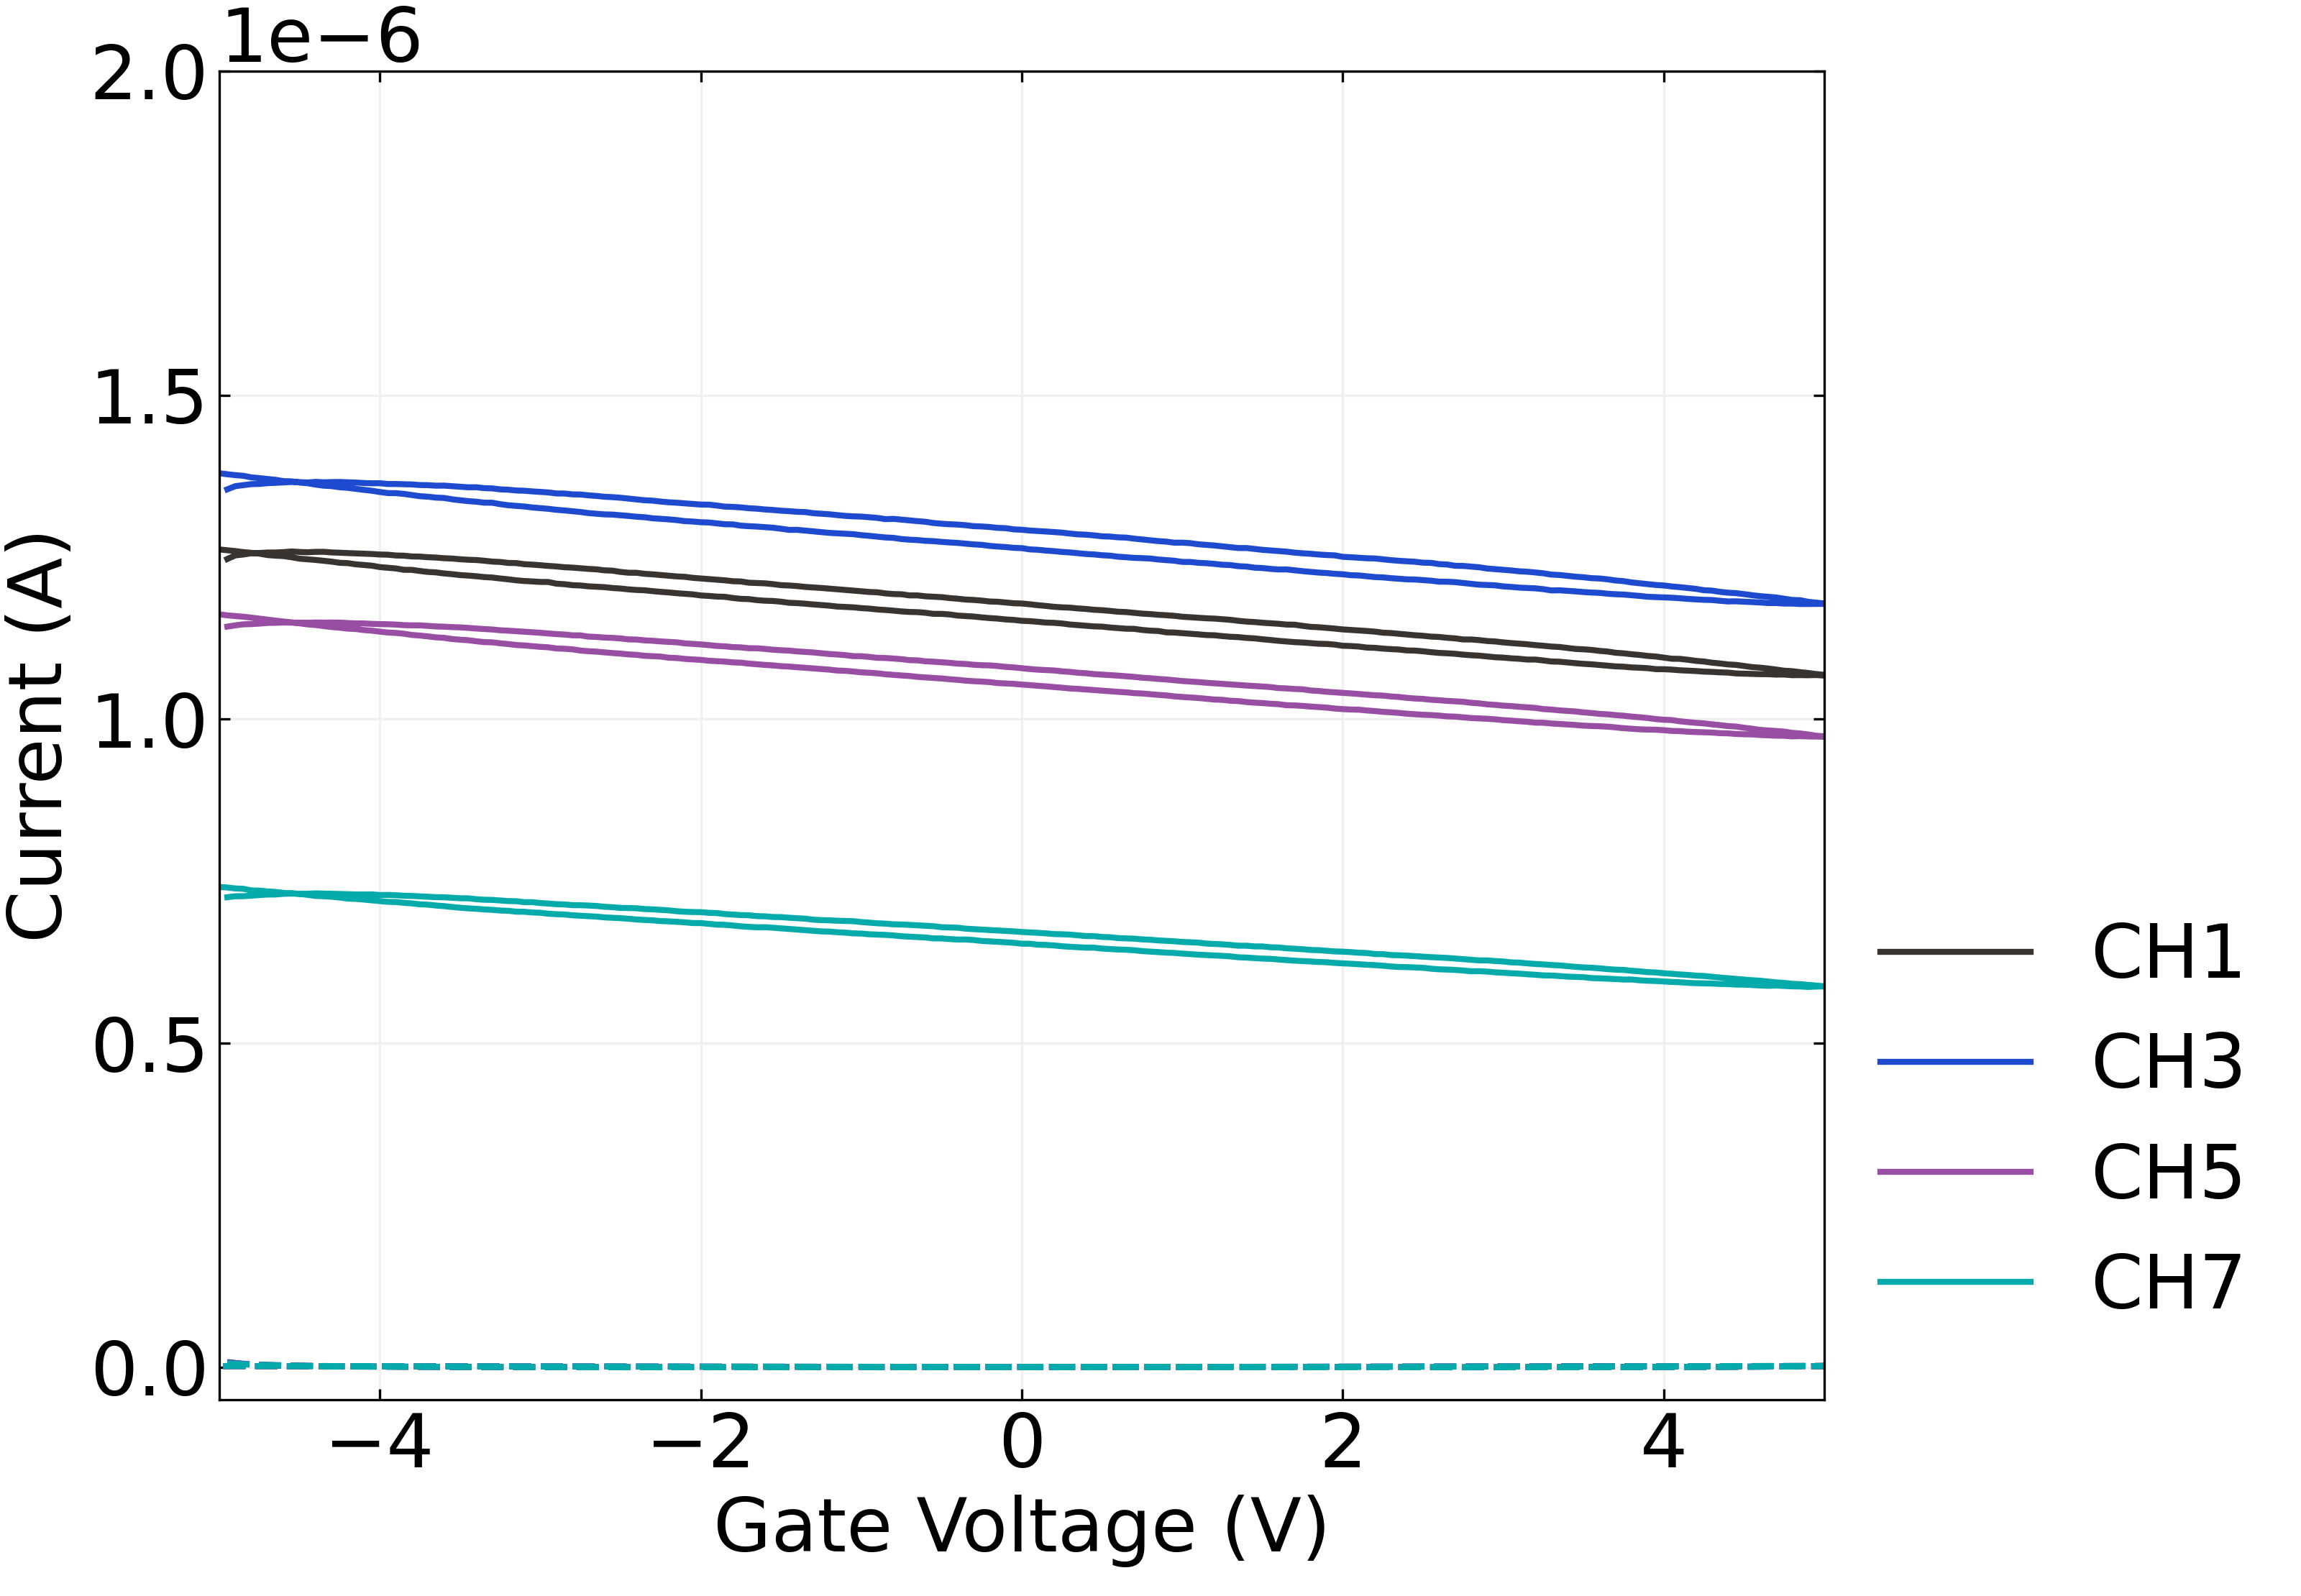
\includegraphics{figures/ch5/Q35C3_nobuffer.png}

}

}

\subcaption{\label{fig-no-buffer}}
\end{minipage}%
%
\begin{minipage}[t]{0.05\linewidth}

{\centering 

~

}

\end{minipage}%
%
\begin{minipage}[t]{0.47\linewidth}

{\centering 

\raisebox{-\height}{

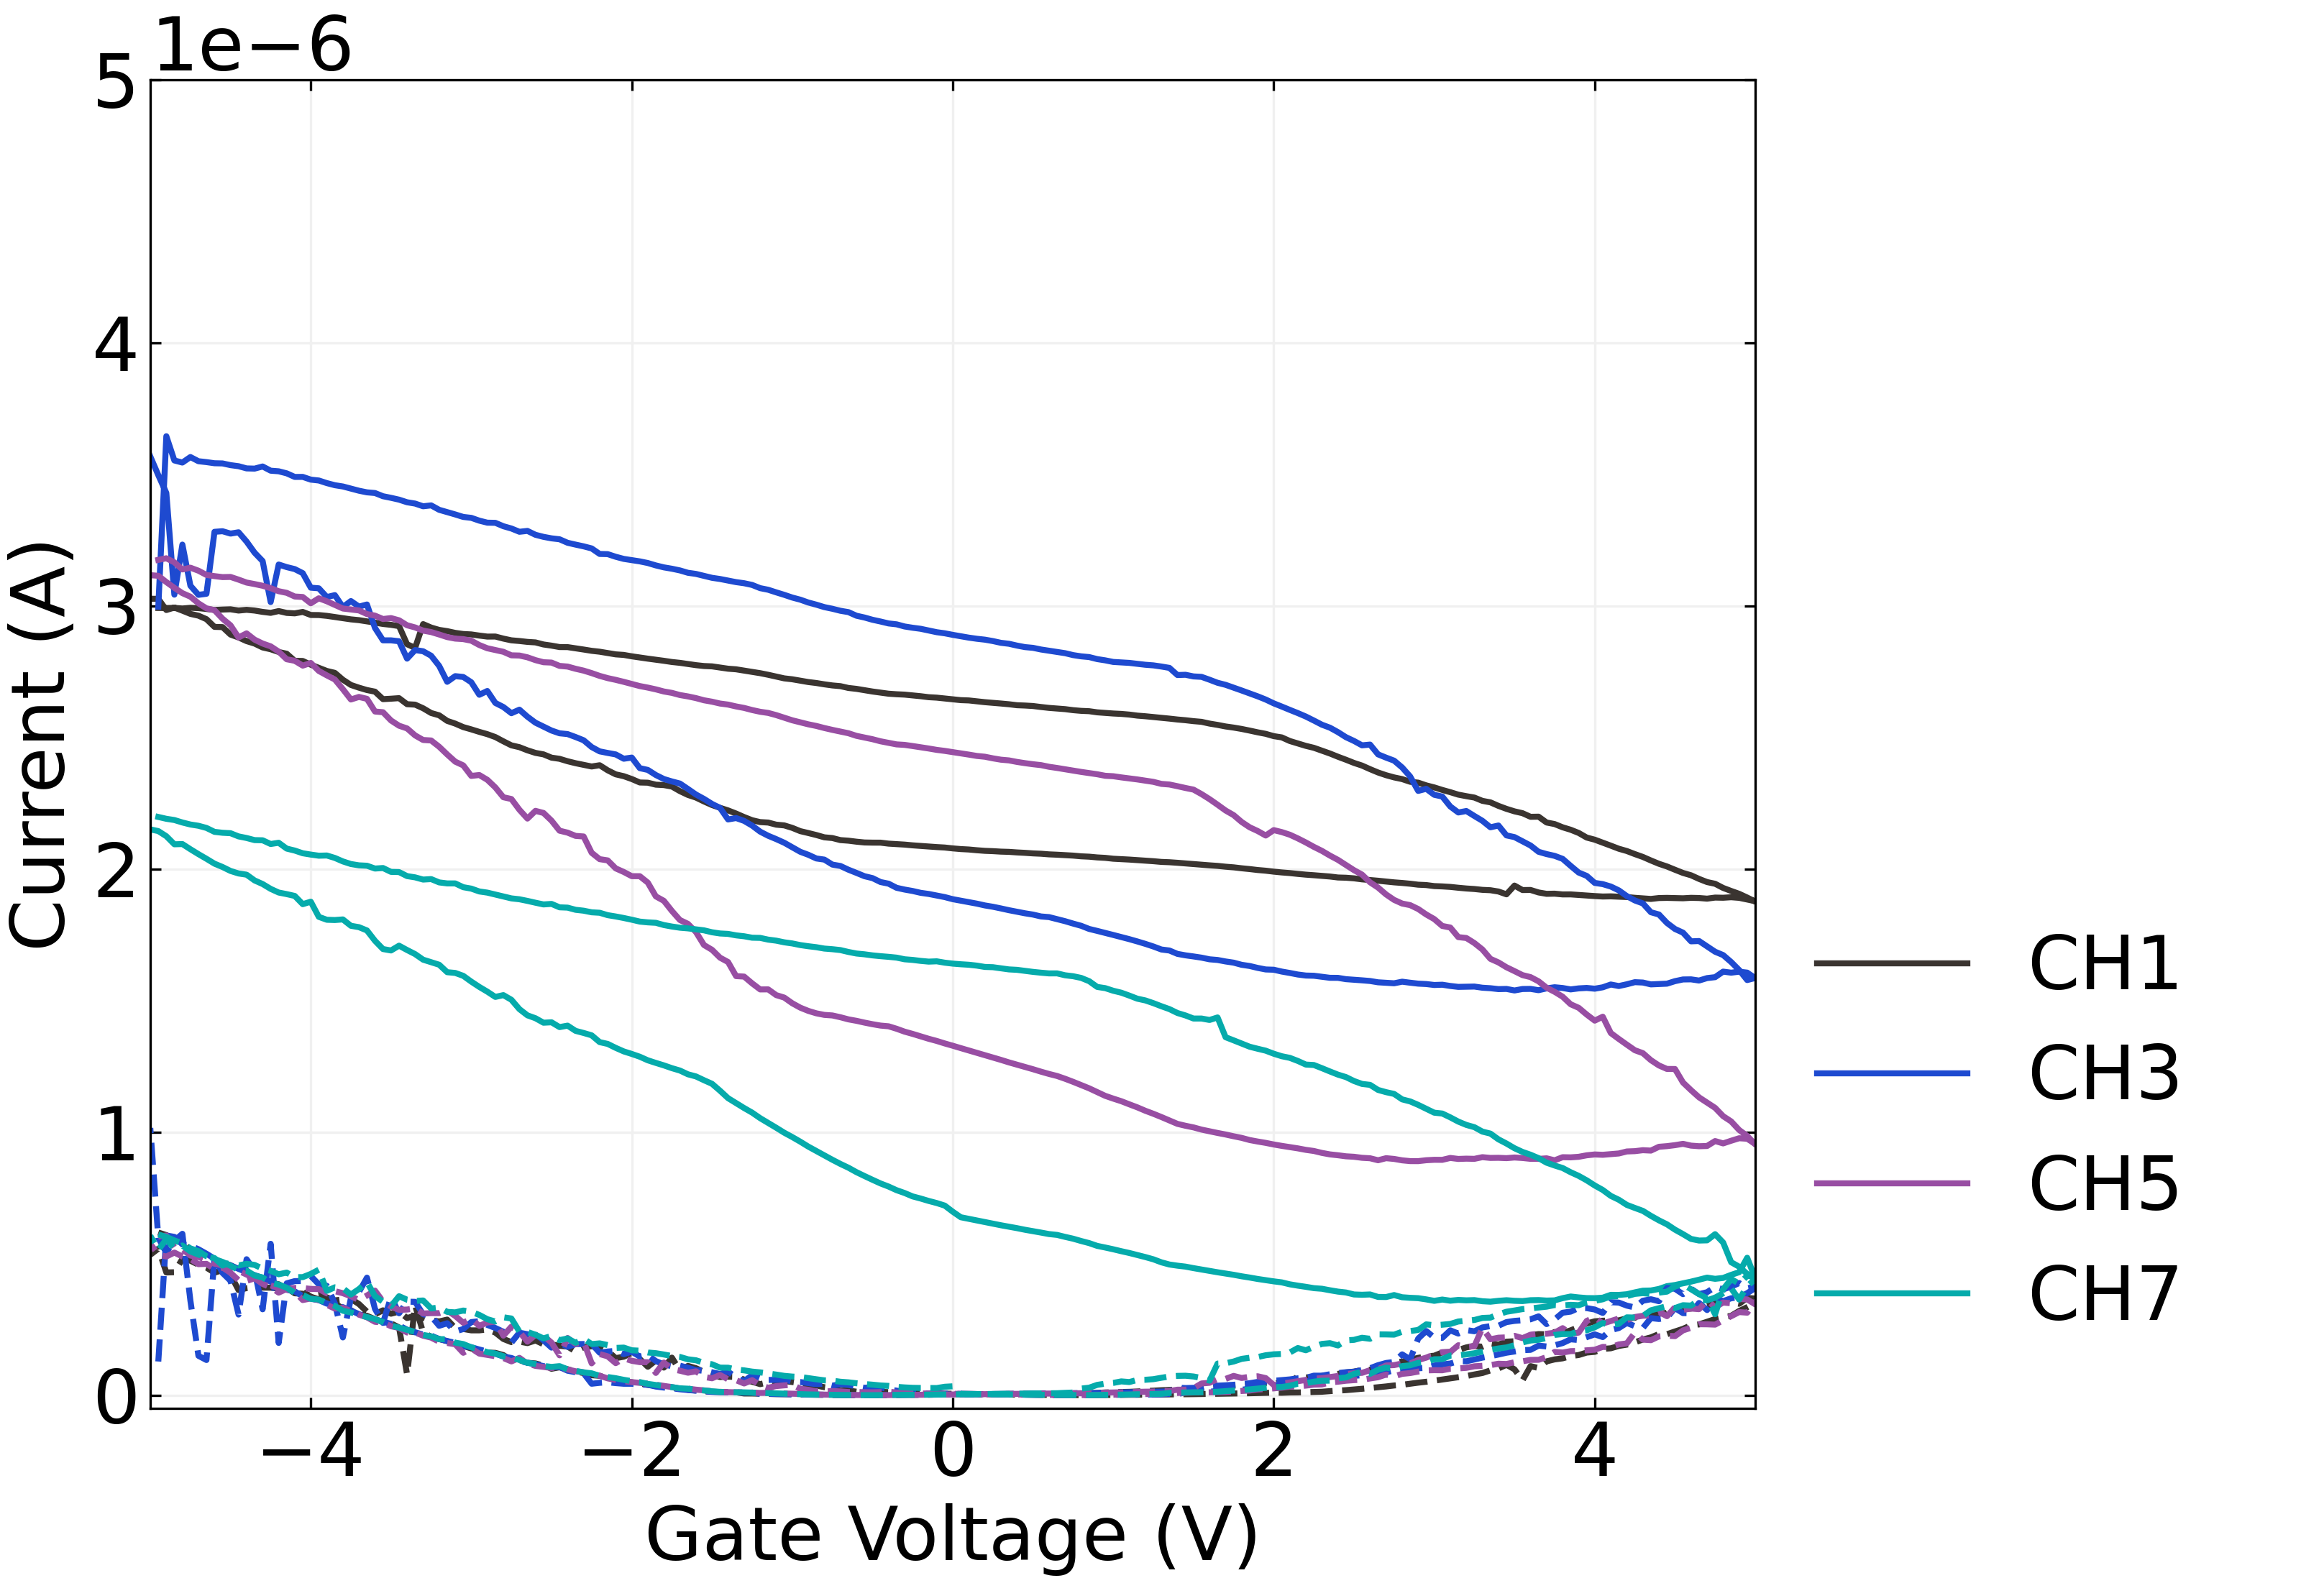
\includegraphics{figures/ch5/Q35C3_buffer.png}

}

}

\subcaption{\label{fig-50uL-buffer}}
\end{minipage}%

\caption{\label{fig-buffer-effect-on-backgate}Backgated transfer sweeps
were taken of an single unencapsulated device with a 300 nm SiO\(_2\)
layer and steam assisted surfactant-deposited carbon nanotube network
channels before and after being covered in \(50 \mu\)L 1XPBS
electrolyte.}

\end{figure}

Figure~\ref{fig-buffer-effect-on-backgate} shows the behaviour of an
unencapsulated backgated device with a 300 nm SiO\(_2\) layer before and
after being covered by 50 \(\mu\)L of 1XPBS (phosphate buffered saline).
The on-off ratio and hysteresis of the channels increase significantly.
The presence of water increases hysteresis through introducing charge
traps at the silicon dioxide surface around the carbon nanotubes and at
the surface of the nanotubes themselves. The use of alternative
transistor dielectrics and/or device functionalisation could potentially
be used to reduce this hysteresis, as the time variation in threshold
voltage due to hysteresis is unwanted for biosensing work
\autocite{Kim2003,Lee2007,Franklin2012,Ha2014}. The electrical double
layer formed by the electrolyte at the surface of the carbon nanotubes
will also have contributed to the observed change in electrical
properties, as it screens surface charge present on the surface around
the nanotubes \autocite{Heller2010}.

There is also a significant increase in current leakage to the backgate
for larger applied voltages, despite the electrolyte having no visible
physical contact with the silicon backgate or copper plane. This leakage
current may simply be due to an increase in relative humidity around the
device due to the presence of water \autocite{Conseil2014}.

\hypertarget{graphene-devices}{%
\subsection{Graphene Devices}\label{graphene-devices}}

\begin{figure}

\begin{minipage}[t]{0.47\linewidth}

{\centering 

\raisebox{-\height}{

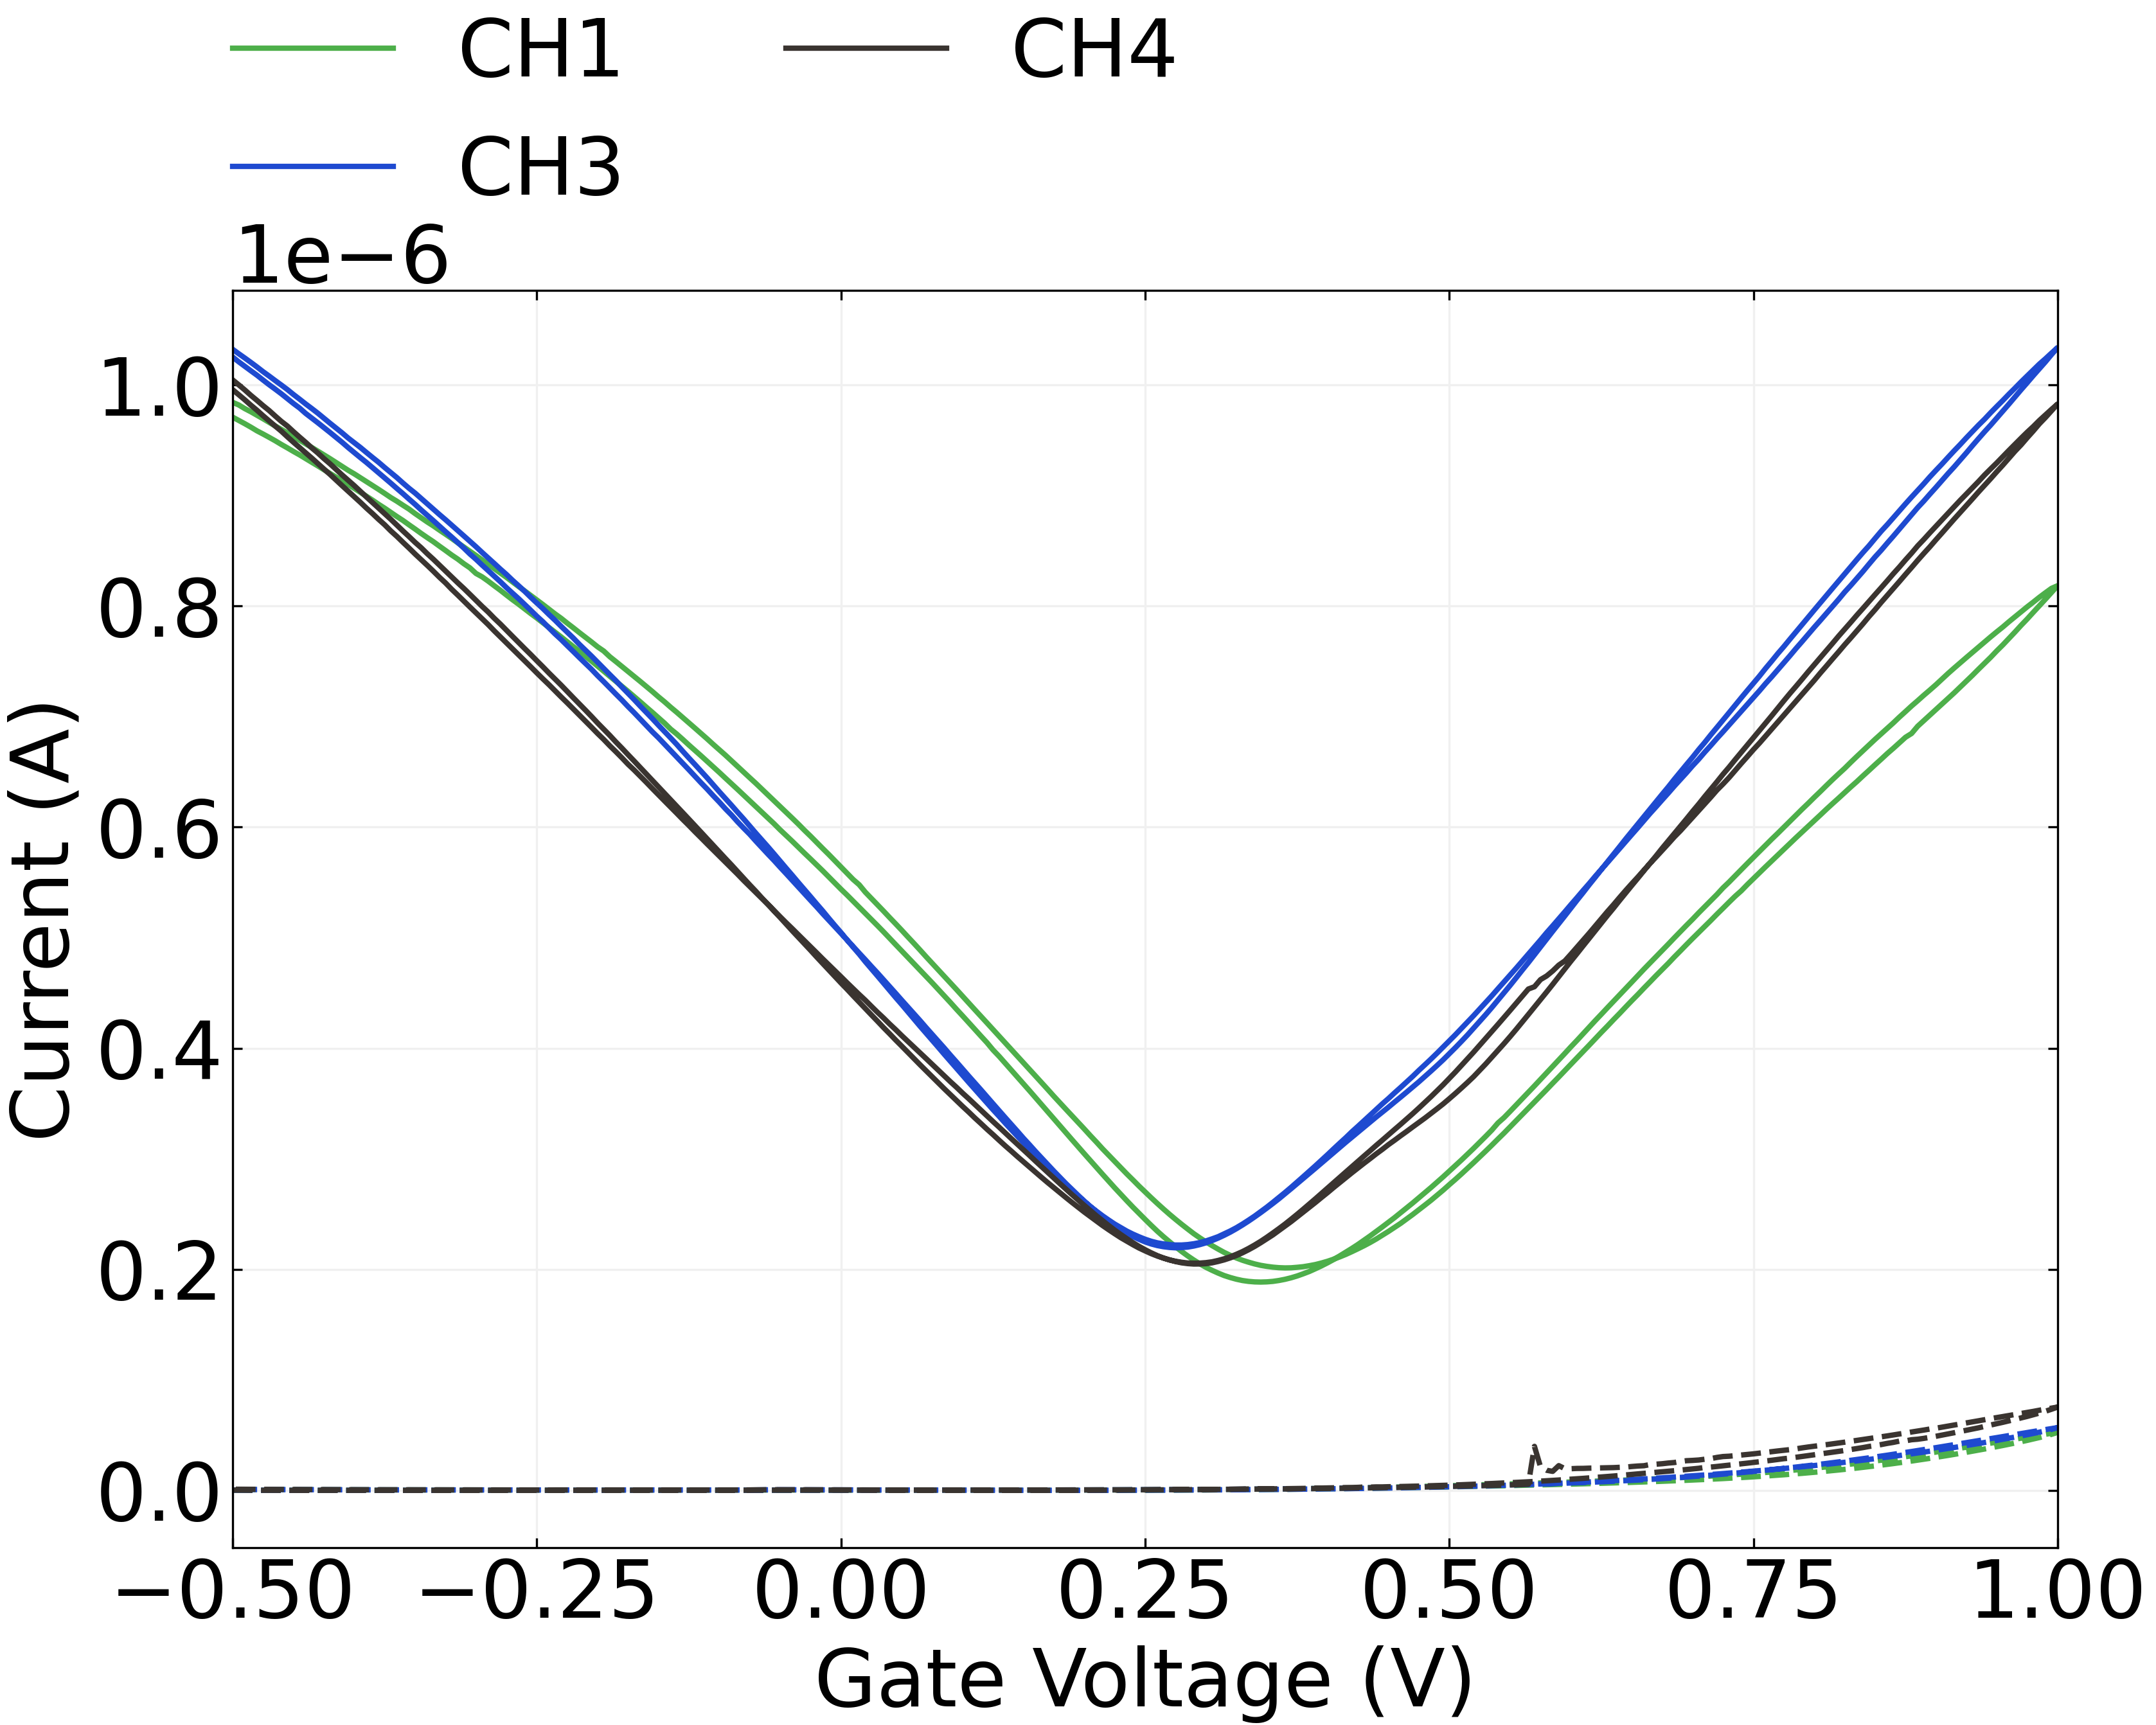
\includegraphics{figures/ch5/JG098_pristine_TXLG01_5mVstep_220920_norinse.png}

}

}

\subcaption{\label{fig-graphene-transfer-1}}
\end{minipage}%
%
\begin{minipage}[t]{0.05\linewidth}

{\centering 

~

}

\end{minipage}%
%
\begin{minipage}[t]{0.47\linewidth}

{\centering 

\raisebox{-\height}{

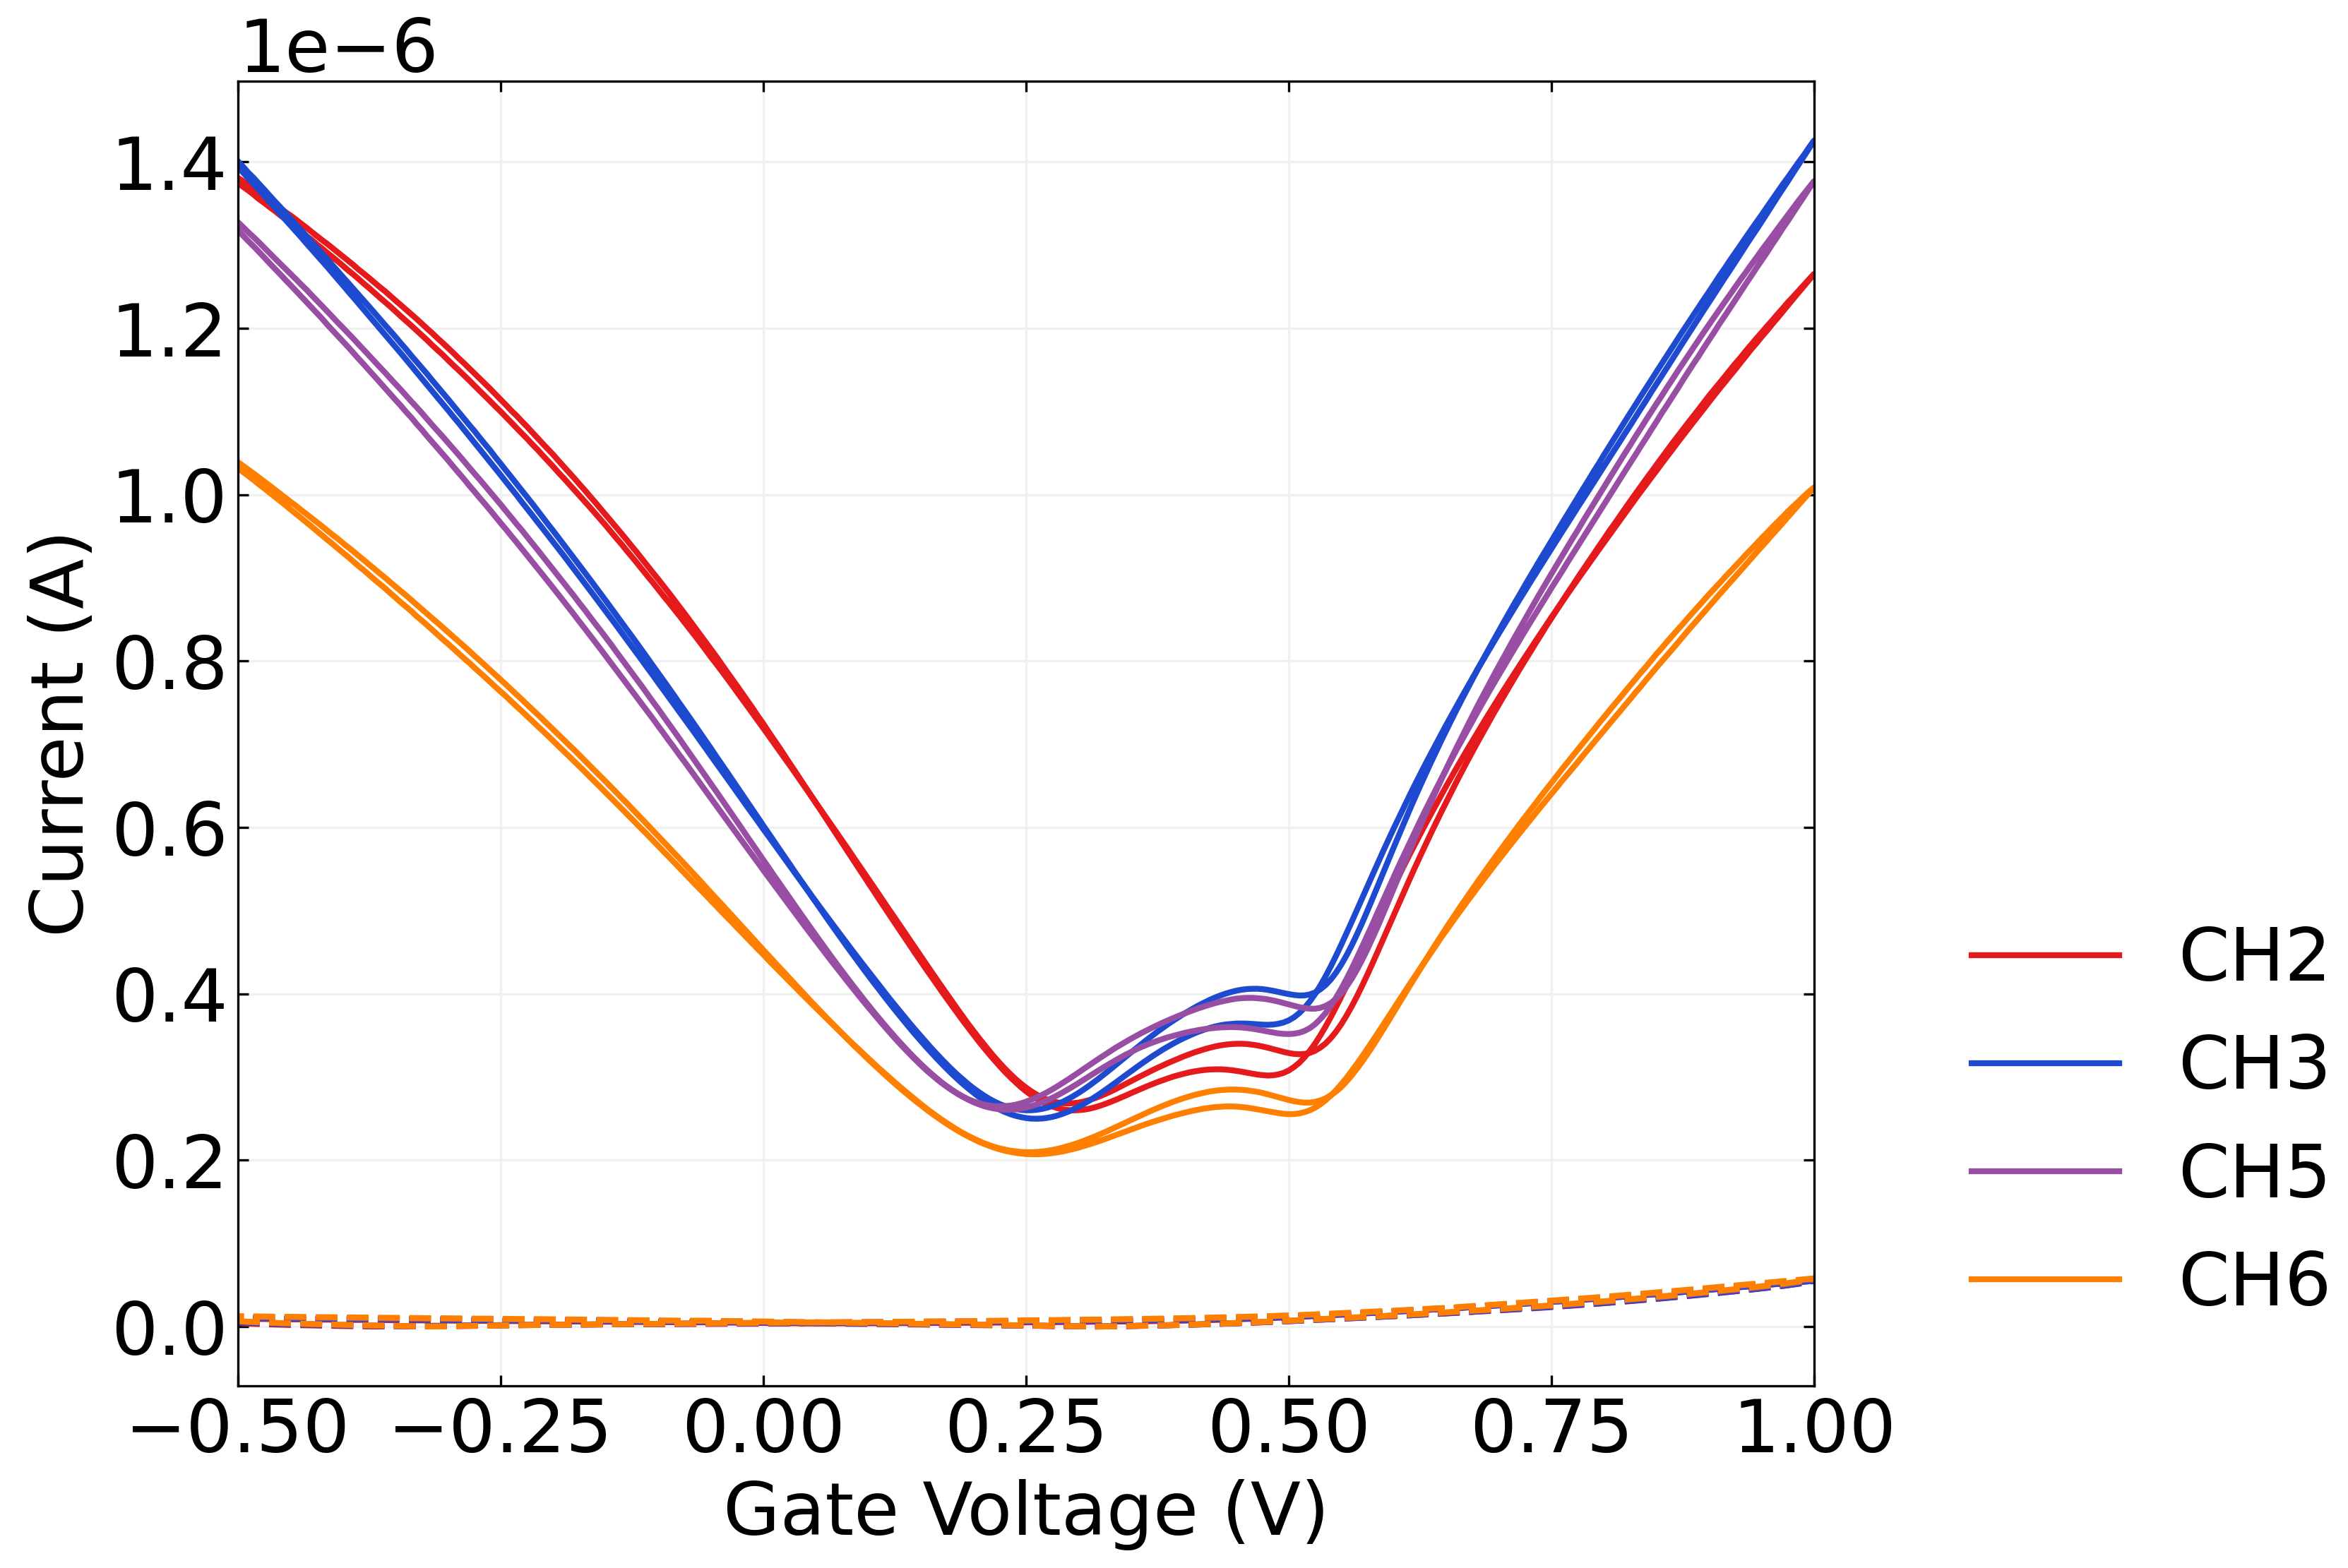
\includegraphics{figures/ch5/JGQ00D6_pristine_TXLG01_5mVstep_220914_norinse.png}

}

}

\subcaption{\label{fig-graphene-transfer-2}}
\end{minipage}%
\newline
\begin{minipage}[t]{0.47\linewidth}

{\centering 

\raisebox{-\height}{

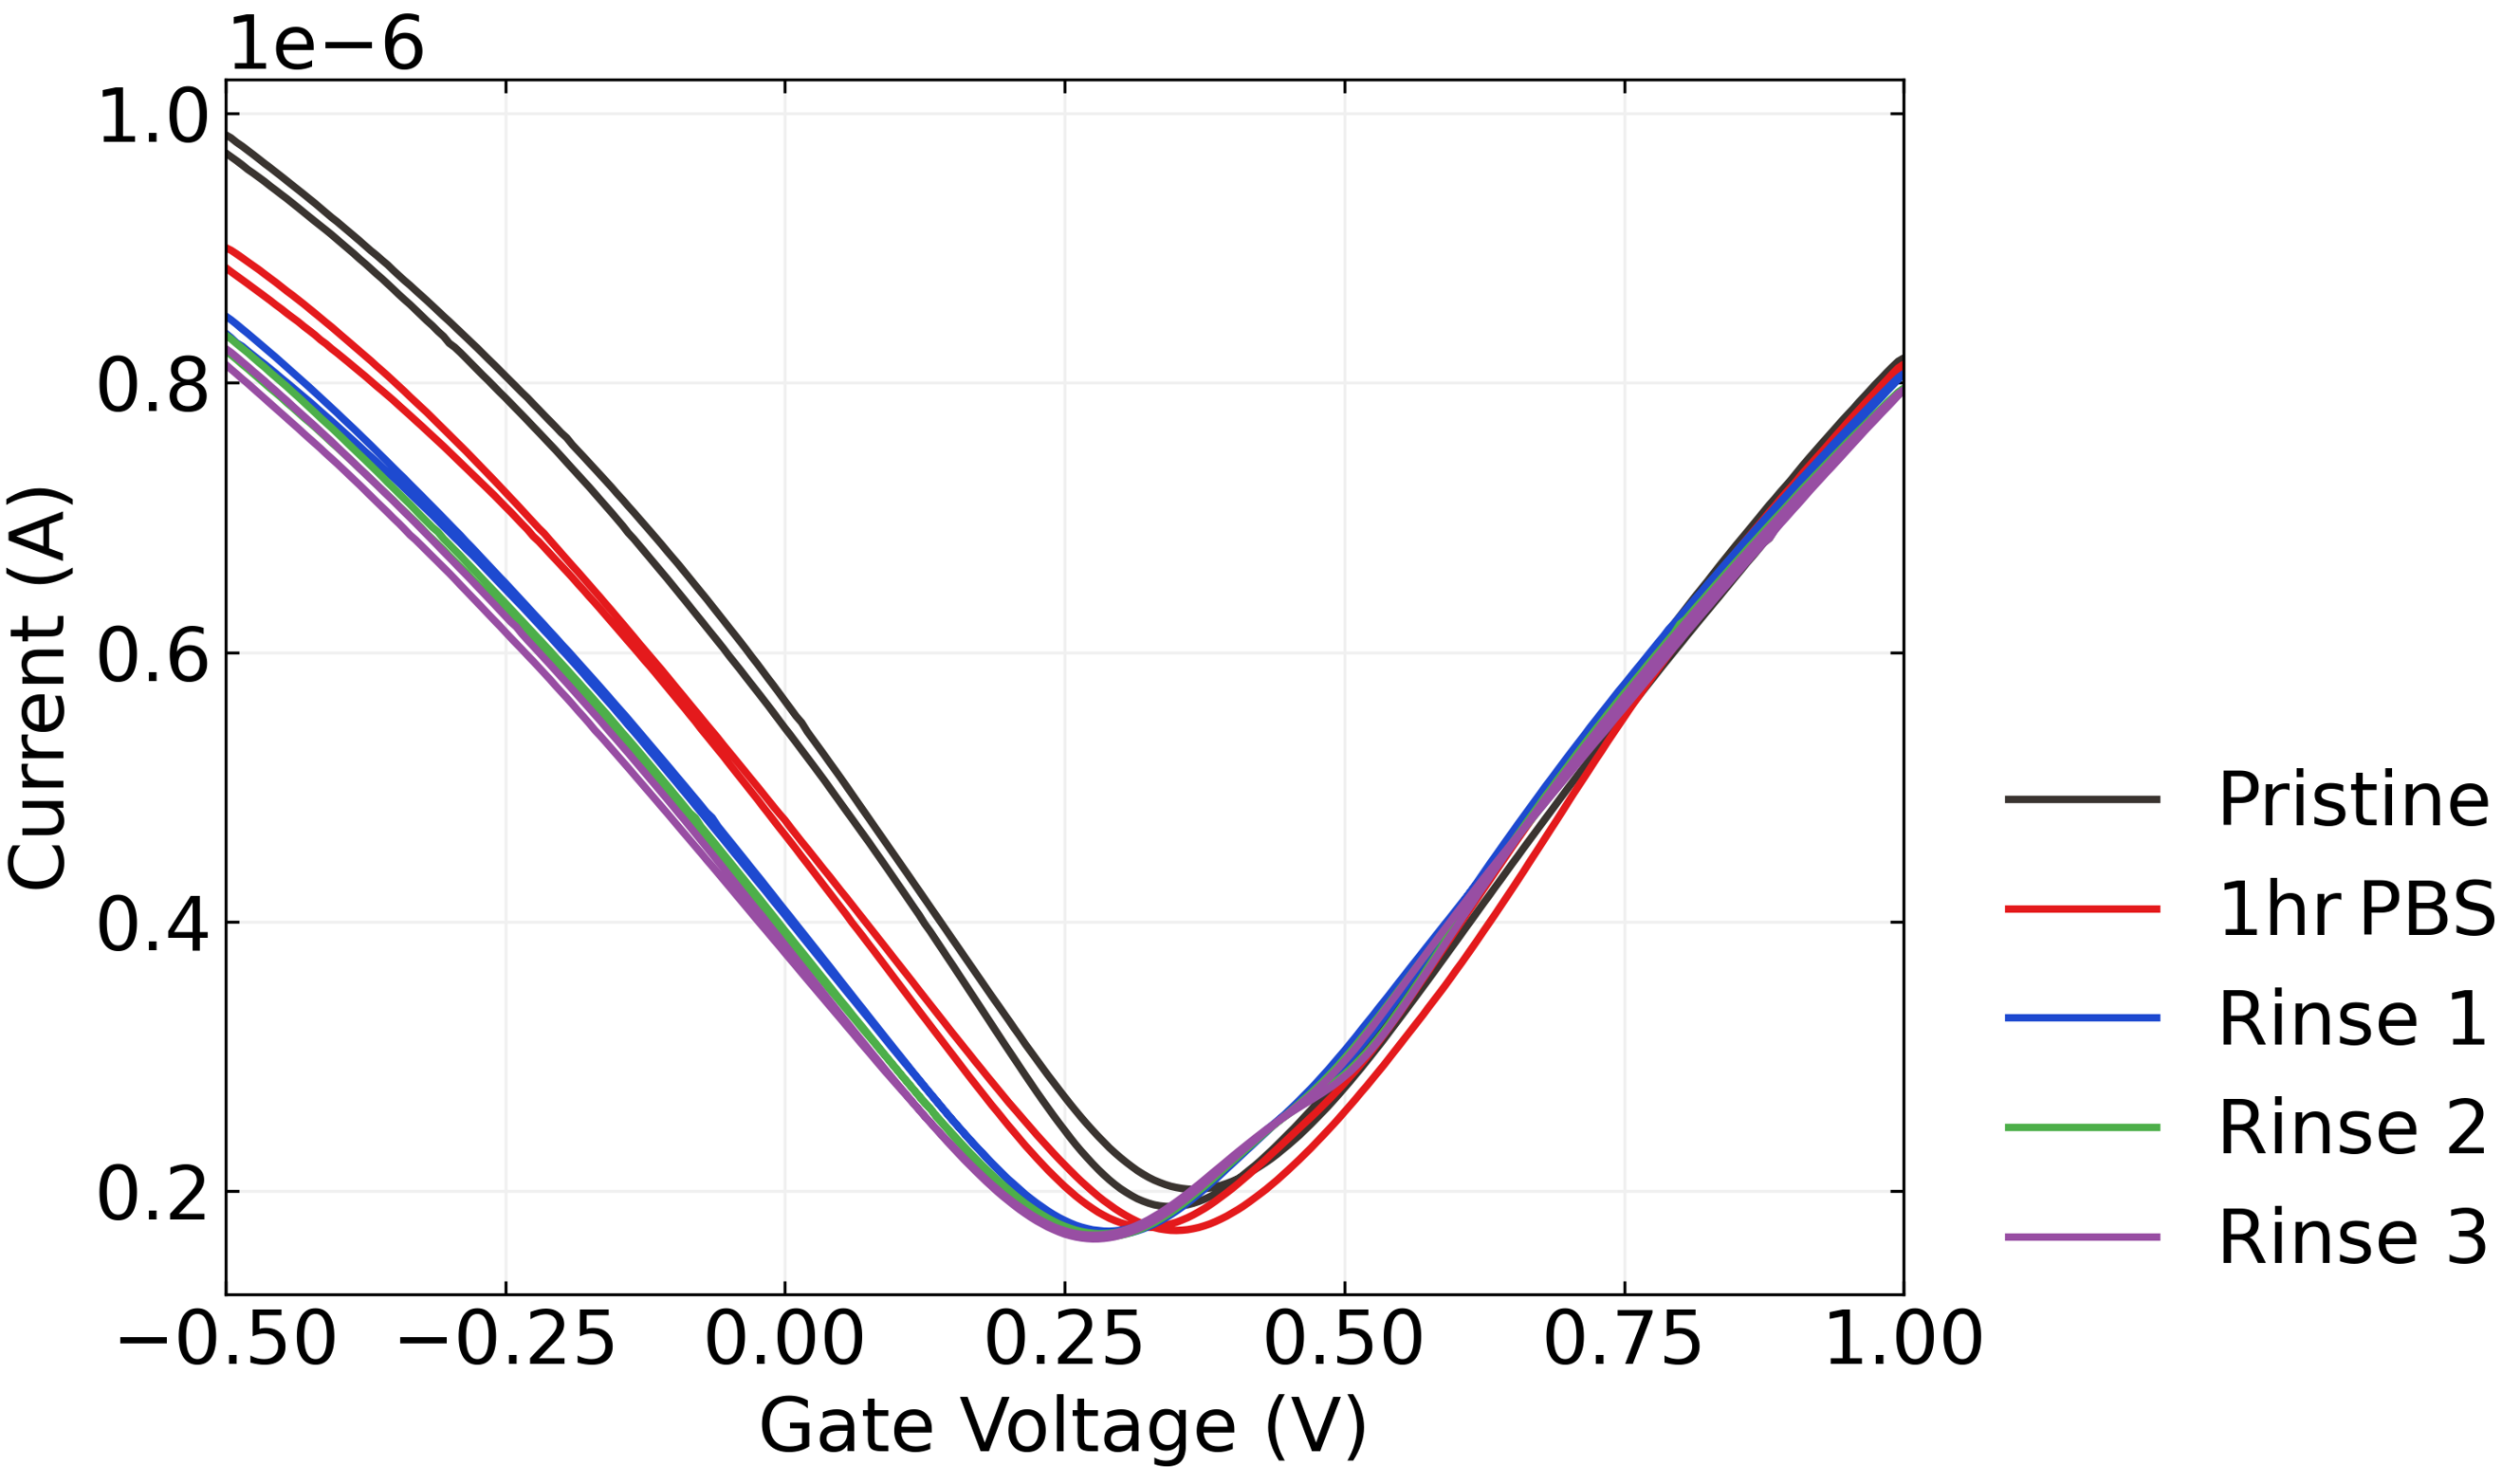
\includegraphics{figures/ch5/JG098_pristine_transfer_sweep_comparison.png}

}

}

\subcaption{\label{fig-graphene-transfer-comparison-1}}
\end{minipage}%
%
\begin{minipage}[t]{0.05\linewidth}

{\centering 

~

}

\end{minipage}%
%
\begin{minipage}[t]{0.47\linewidth}

{\centering 

\raisebox{-\height}{

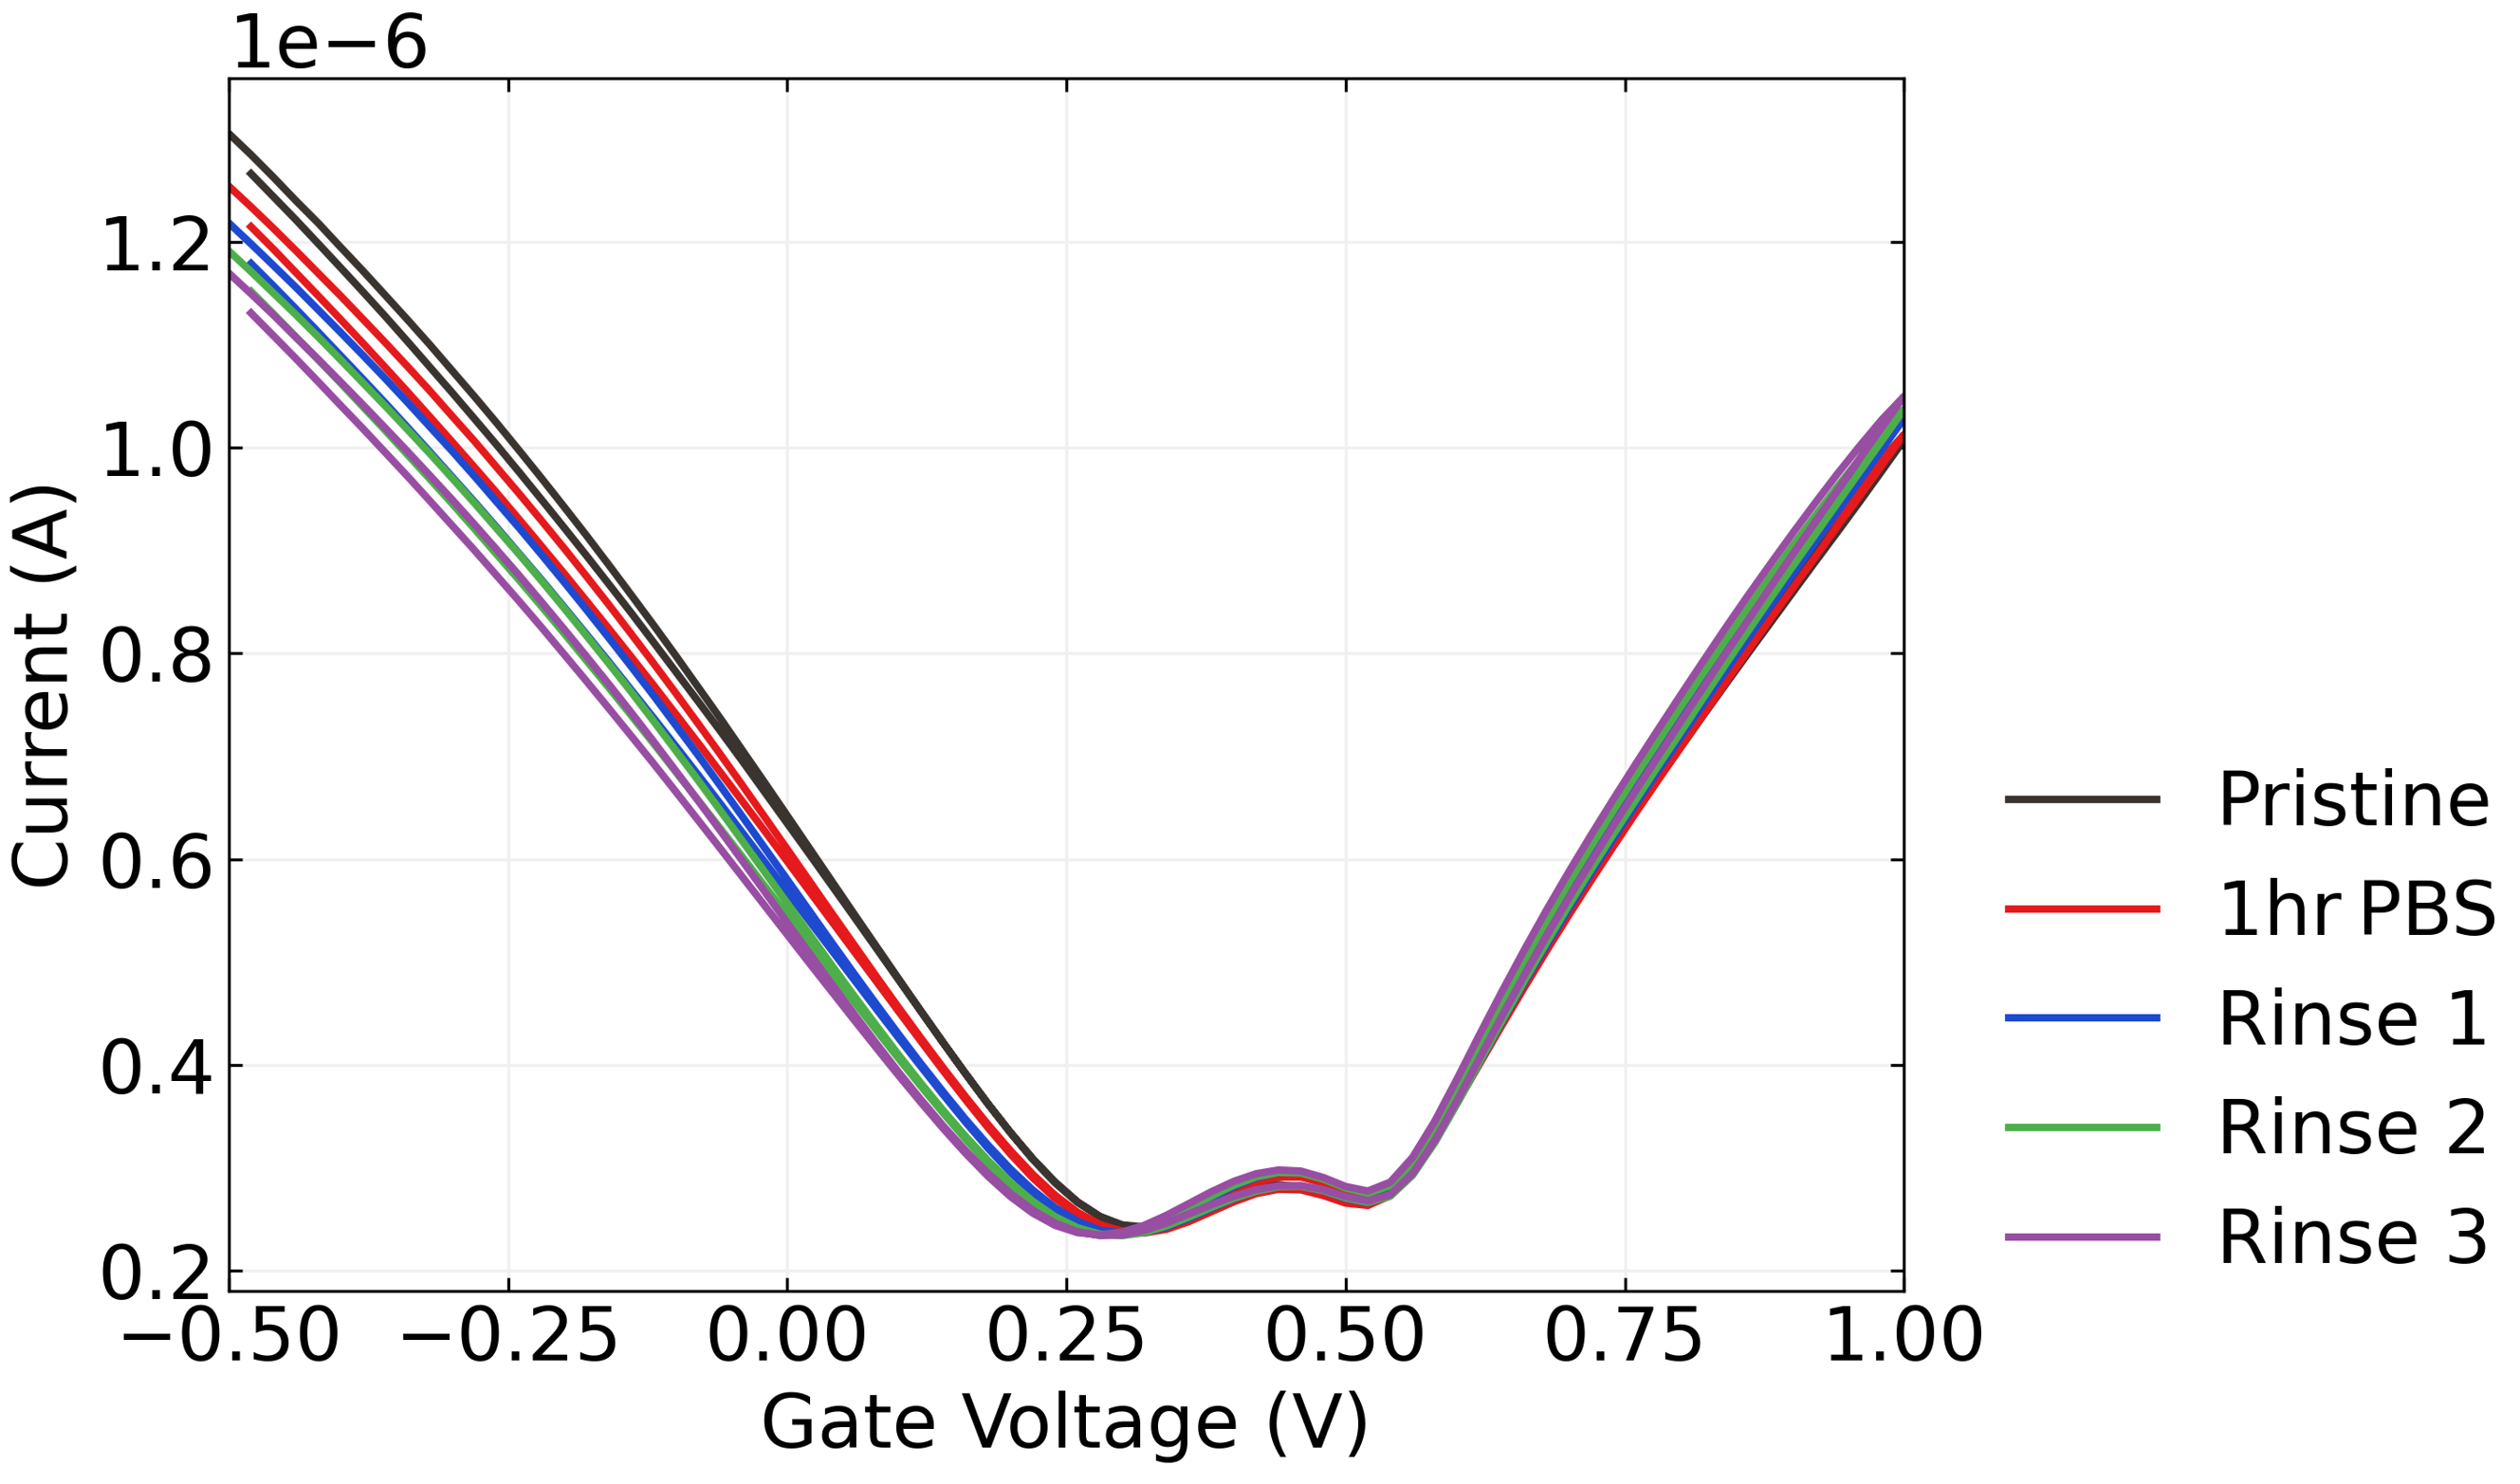
\includegraphics{figures/ch5/JGQ00D6_pristine_transfer_sweep_comparison.png}

}

}

\subcaption{\label{fig-graphene-transfer-comparison-2}}
\end{minipage}%

\caption{\label{fig-pristine-graphene}These figures show liquid-gated
transfer characteristics of channels from two AZ\(^\circledR\) 1518
encapsulated graphene devices. In (a) and (b), the characteristics of
working device channels upon initial exposure to 1XPBS are displayed
alongside gate current. The transfer characteristics of channel 1 in (a)
and channel 5 in (b) after various degrees of exposure to 1XPBS are
shown in (c) and (d) respectively.}

\end{figure}

Graphene devices were electrically characterised in the manner described
in \textbf{?@sec-electrical-characterisation} and analysed using the
Python code discussed in
Section~\ref{sec-field-effect-transistor-analysis}.

Figure~\ref{fig-pristine-graphene} shows the liquid-gated transfer
characteristics of two graphene devices. These devices were fabricated
prior to Jun 2021. Both devices exhibit the ambipolar characteristics
typical of liquid-gated graphene devices
\autocite{Heller2009a,Heller2010,Xia2010,Kireev2017}. As with the carbon
nanotube network devices, leakage current remained below \(\sim\) 1
\(\times\) \(10^{-7}\) V across both the forward and reverse sweep.
Hysteresis between the forward and reverse sweep is caused by trapping
of charge within and on the surface of the SiO\(_{2}\) dielectric
\autocite{Bartolomeo2011}. The major Dirac point for these devices is
slightly to the right of V\(_{\textrm{Dirac}} \approxeq\) 0 V, which
indicates \(p\)-doping of the channel. This slight \(p\)-doping is
likely a result of a adsorption of oxygen and water from the air and
residue resist from photolithography
\autocite{Cheng2011,Shin2012,Kireev2017}.

Some devices exhibited a double-minima feature, indicating the presence
of two Dirac points. This effect arises due to doping of graphene by the
metal contacts. In shorter length channels, metal doping affects the
entire channel length, leading to a consistent Fermi level and a single
Dirac point. However, for longer channel lengths like ours, the doping
effect from metal contact no longer reaches the entire channel, leading
to a difference in Fermi level between the graphene in the channel and
graphene under the metal contact. The difference in Fermi levels results
in the presence of a second Dirac point
\autocite{Bartolomeo2011,Feng2014,Peng2018}. The global minimum of the
transfer characteristic can be referred to as the `major' Dirac point.

Figure~\ref{fig-pristine-graphene} also shows the effect of 1XPBS on the
graphene channels. The channels were measured on exposure to 1XPBS,
after exposure to 1XPBS for one hour, and after the device surface was
rinsed and 1XPBS was replaced in the well one time, two times and three
times successively. A slight negative shift of the major Dirac point was
observed. This effect is possibly a result of gate bias stress, where
successive transfer sweeps introduce charge traps to the graphene layer
and alters the current level at a given gate voltage
\autocite{Bargaoui2018,Noyce2019}. Alternatively, Kireev \emph{et al.}
found that a series of liquid-gated sweeps also reduced the size of the
second Dirac point, and suggested that it indicated the gate current was
removing atmospheric contaminants from the graphene surface via current
annealing \autocite{Kireev2017}. This could be explained as the removal
of contaminants causing improved contact between the metal and graphene
surface, and thus increasing metal doping and consistency of the Fermi
level across the channel. If the contaminants removed are \(p\)-dopants,
then this effect could also explain the negative shift of the major
Dirac point.

\hypertarget{tbl-graphene-parameters}{}
\begin{table}
\caption{\label{tbl-graphene-parameters}Average on-off ratio and major Dirac point voltage for AZ® 1518
encapsulated liquid-gated graphene transistor channels at various stages
of exposure to 1XPBS. Electrical characteristics were taken of 6
channels total, three channels from each of two devices. }\tabularnewline

\centering
\begin{tabular}{lccc}
\toprule
 & 1XPBS: Initial & 1XPBS: After 1 hr & 1XPBS: Rinse\\
\midrule
On-Off Ratio (arb.) & 5.1 ± 0.3 & 5.0 ± 0.7 & 5.0 ± 0.6\\
Dirac Point Voltage (V) & 0.28 ± 0.04 & 0.31 ± 0.03 & 0.28 ± 0.02\\
\bottomrule
\end{tabular}
\end{table}

Table~\ref{tbl-graphene-parameters} shows the on-off ratio and major
Dirac point voltage of the graphene devices. Apart from the
previously-mentioned slight negative shift of the major Dirac point,
these values were highly consistent before and after exposure to 1XPBS.

\hypertarget{sec-dummy-sensing}{%
\section{Real-Time Salt Concentration Sensing with Phosphate Buffered
Saline}\label{sec-dummy-sensing}}

All devices analysed in this section were fabricated using
steam-assisted, surfactant-deposited carbon nanotube network films.

\hypertarget{sec-baseline-drift}{%
\subsection{Control Series and Baseline
Drift}\label{sec-baseline-drift}}

The total interval for the control series was 1800 s, with 20\(\mu\)L
1XPBS additions at 100 s, 200 s and 300 s, and 20\(\mu\)L subtractions
at 400 s, 500 s and 600 s. Devices were left untouched over the next
1200 s to allow the current level to settle.
Figure~\ref{fig-transfer-sweep} shows the transfer sweep of a single
channel of a steam-assisted surfactant-deposited device encapsulated
with SU8, fabricated after Jun 2023. The threshold voltage of the
channel is \(V_{\textrm{th}}\) = 140 mV, and the voltage corresponding
to minimum current is \(V_{\textrm{gap}}\) = 310 mV. The variable symbol
V\(_{\textrm{gap}}\) denotes the center of the transistor bandgap, has
been labeled in this manner to be consistent with previous work
\autocite{Heller2009}.

\begin{figure}

\begin{minipage}[t]{0.45\linewidth}

{\centering 

\raisebox{-\height}{

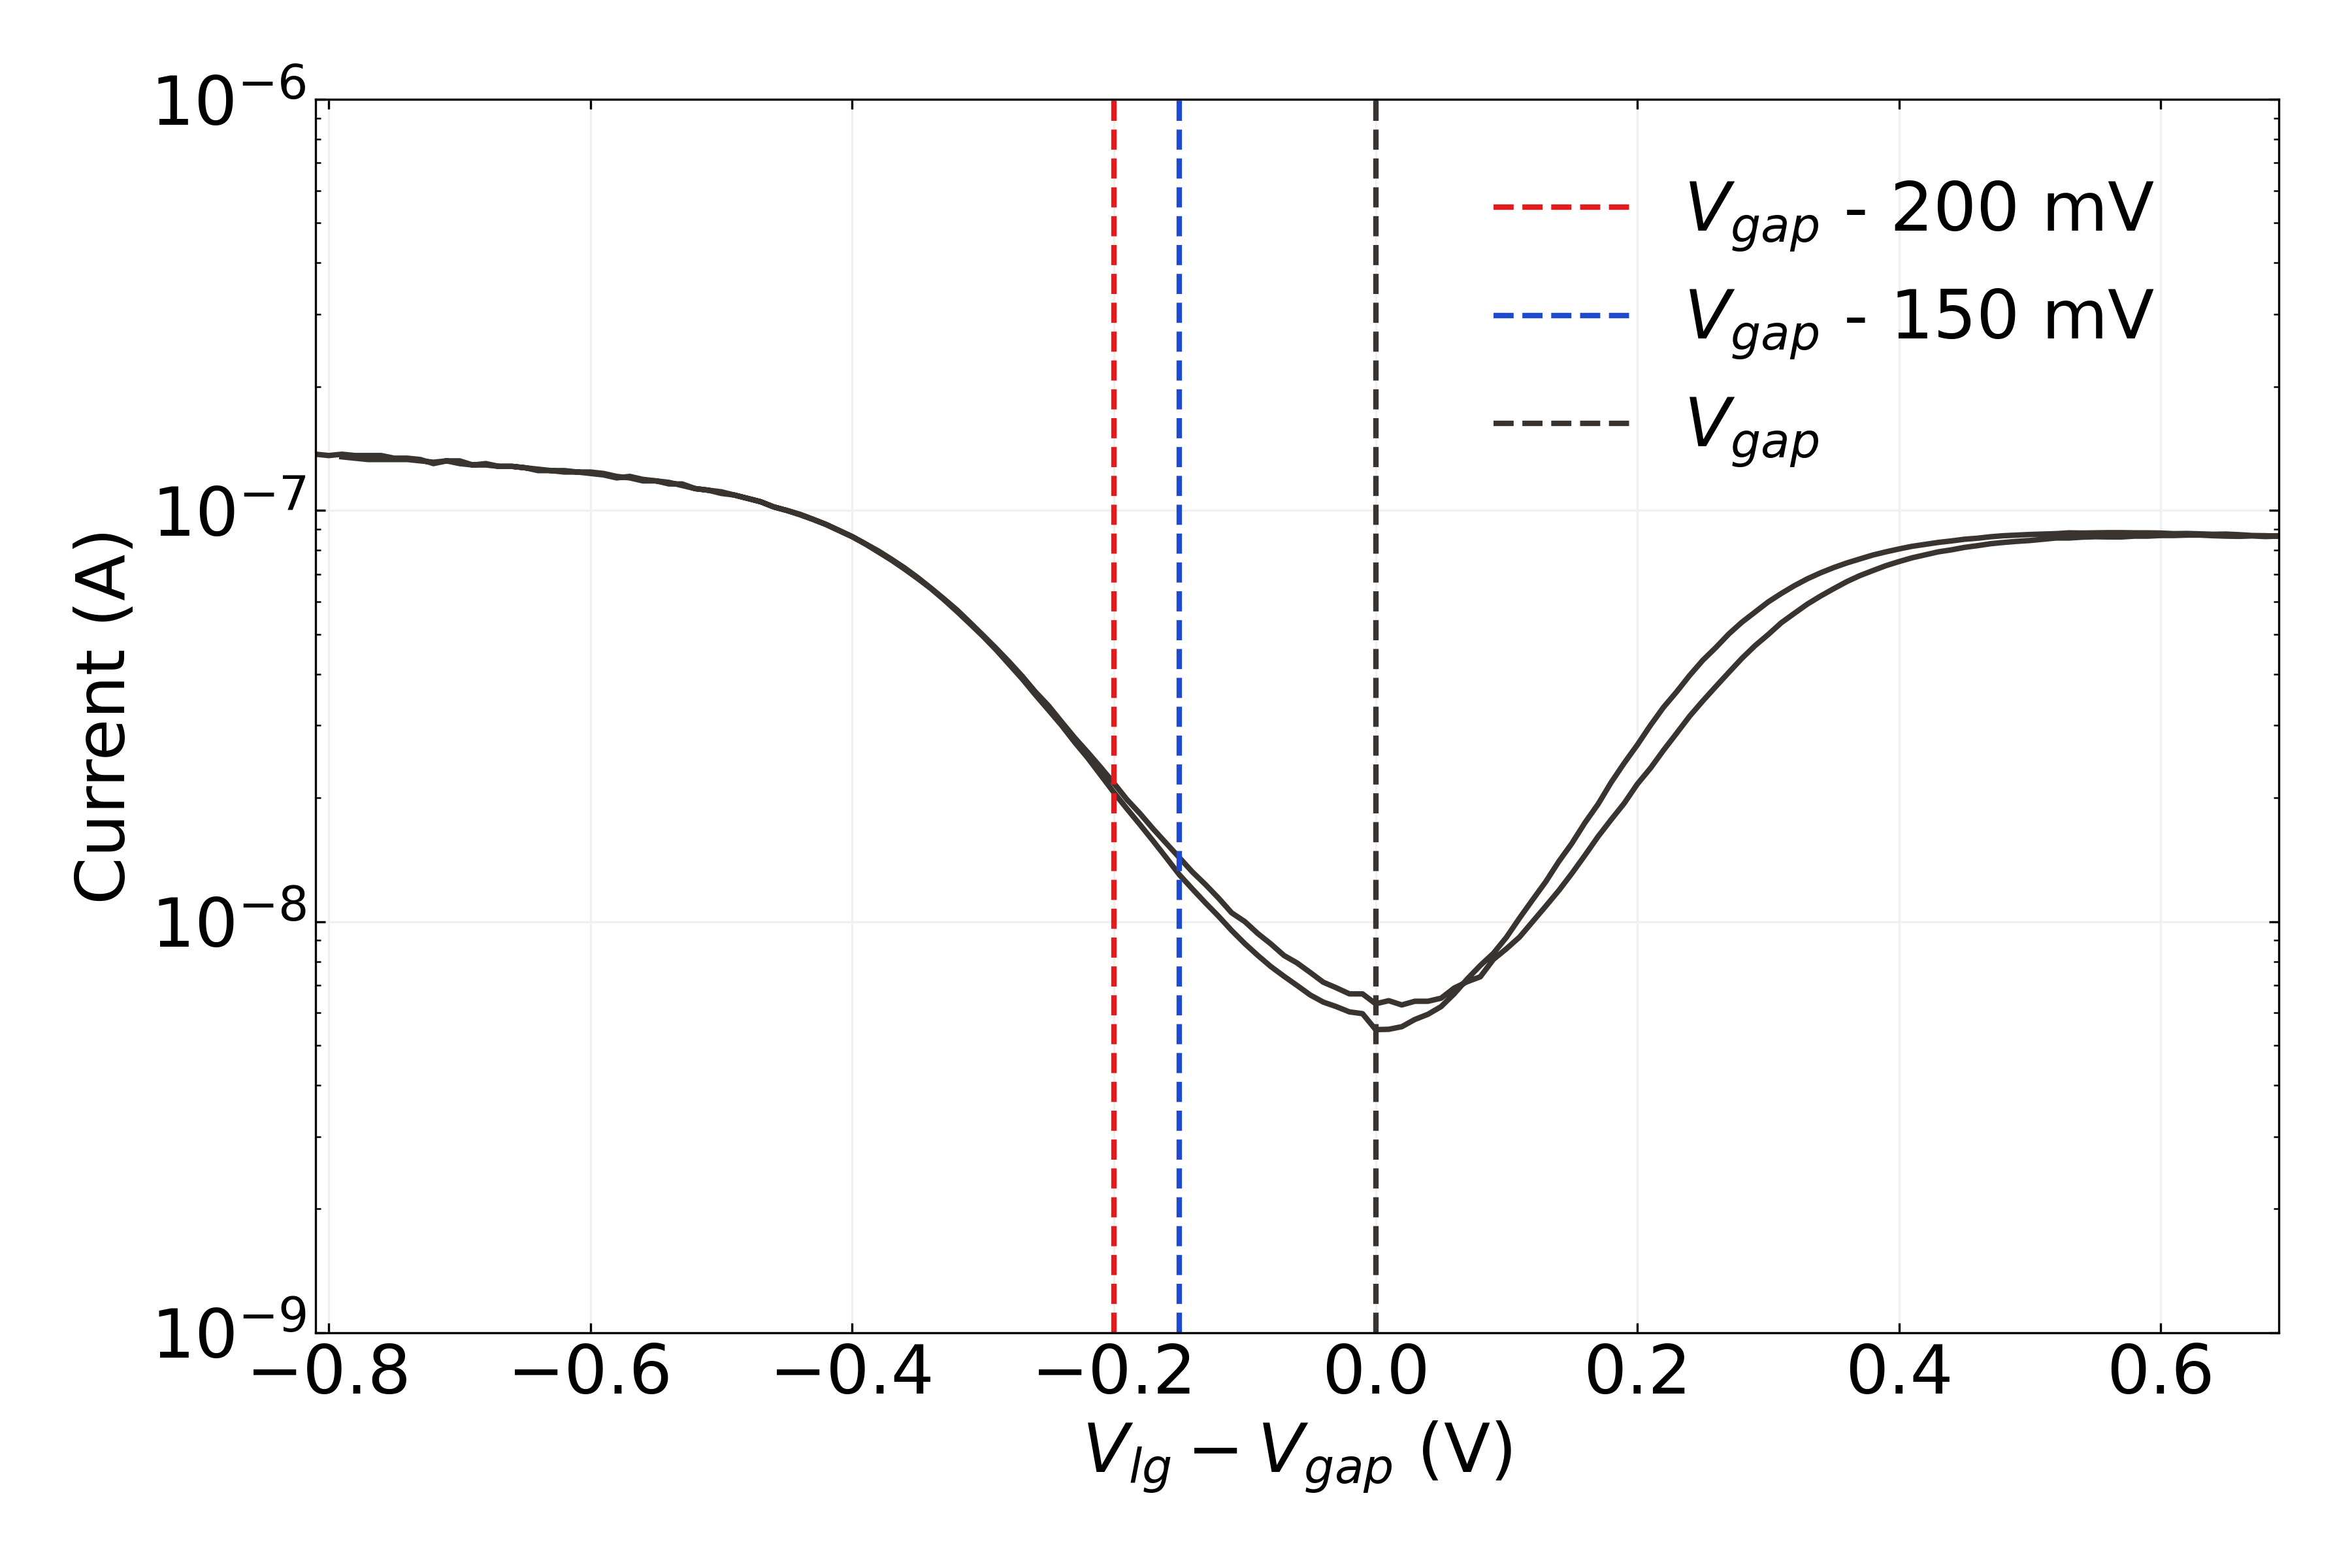
\includegraphics{figures/ch5/Q2C10ch8custom.png}

}

}

\subcaption{\label{fig-transfer-sweep}}
\end{minipage}%
%
\begin{minipage}[t]{0.05\linewidth}

{\centering 

~

}

\end{minipage}%
%
\begin{minipage}[t]{0.50\linewidth}

{\centering 

\raisebox{-\height}{

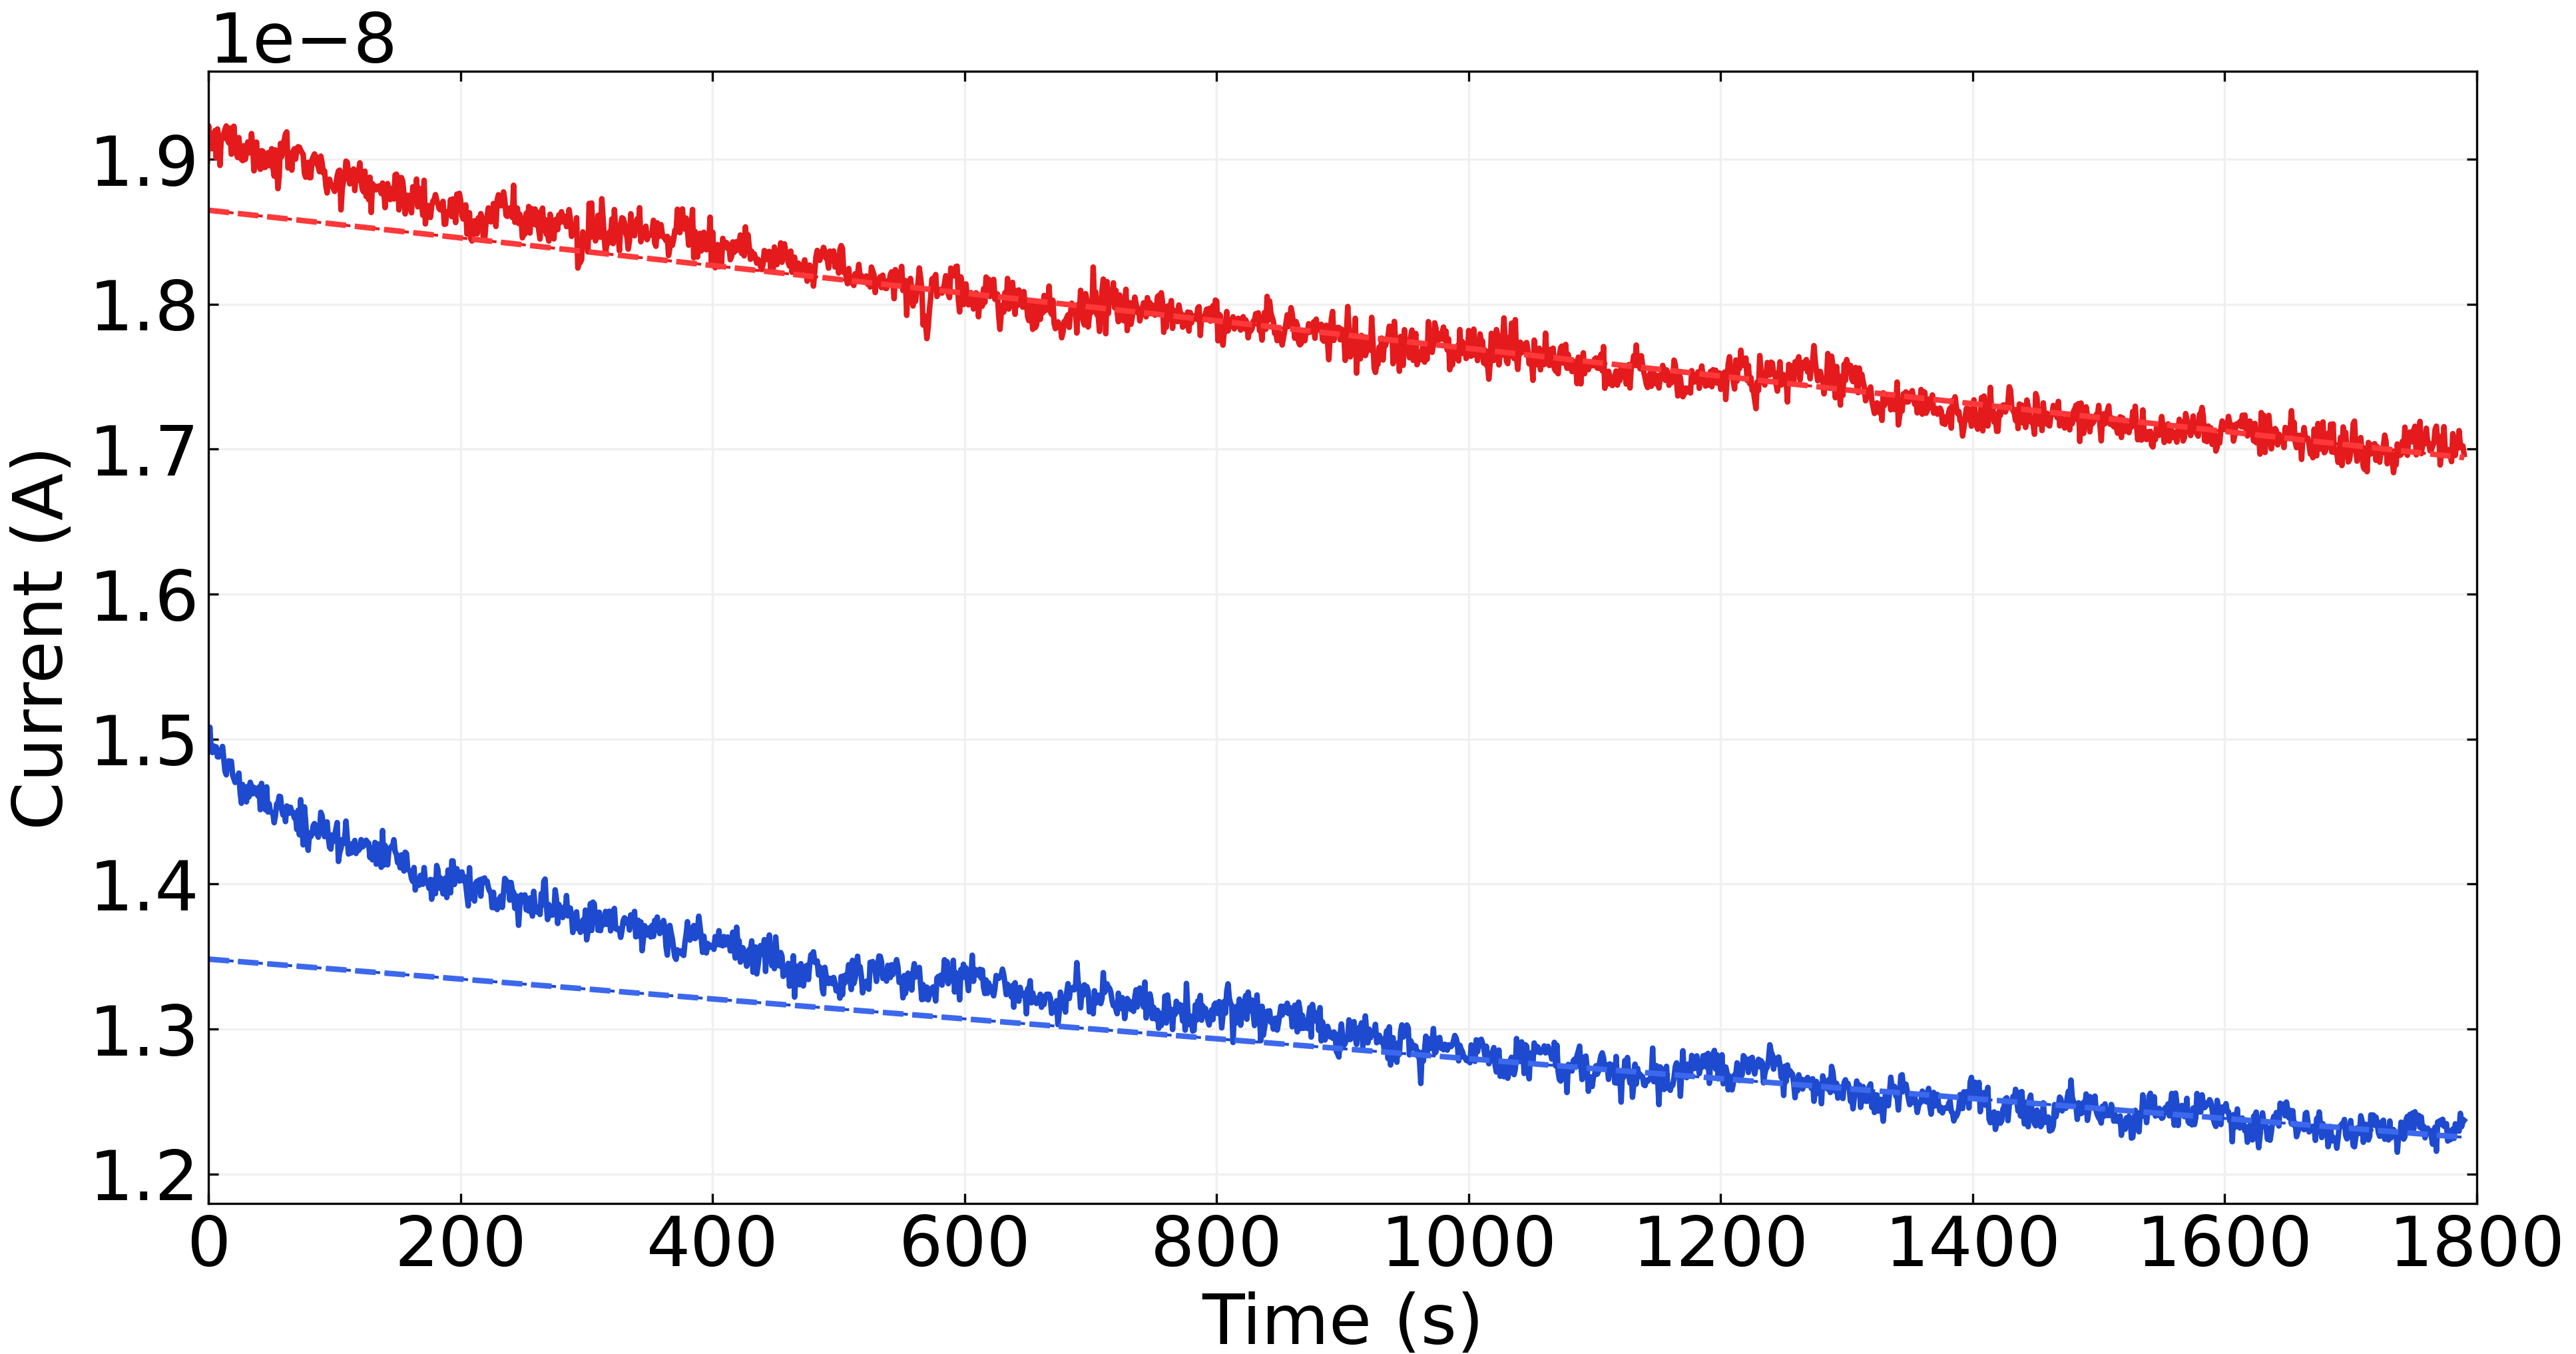
\includegraphics{figures/ch5/Q2C10_with_fitted_curves.png}

}

}

\subcaption{\label{fig-linear-fit}}
\end{minipage}%
\newline
\begin{minipage}[t]{0.25\linewidth}

{\centering 

~

}

\end{minipage}%
%
\begin{minipage}[t]{0.50\linewidth}

{\centering 

\raisebox{-\height}{

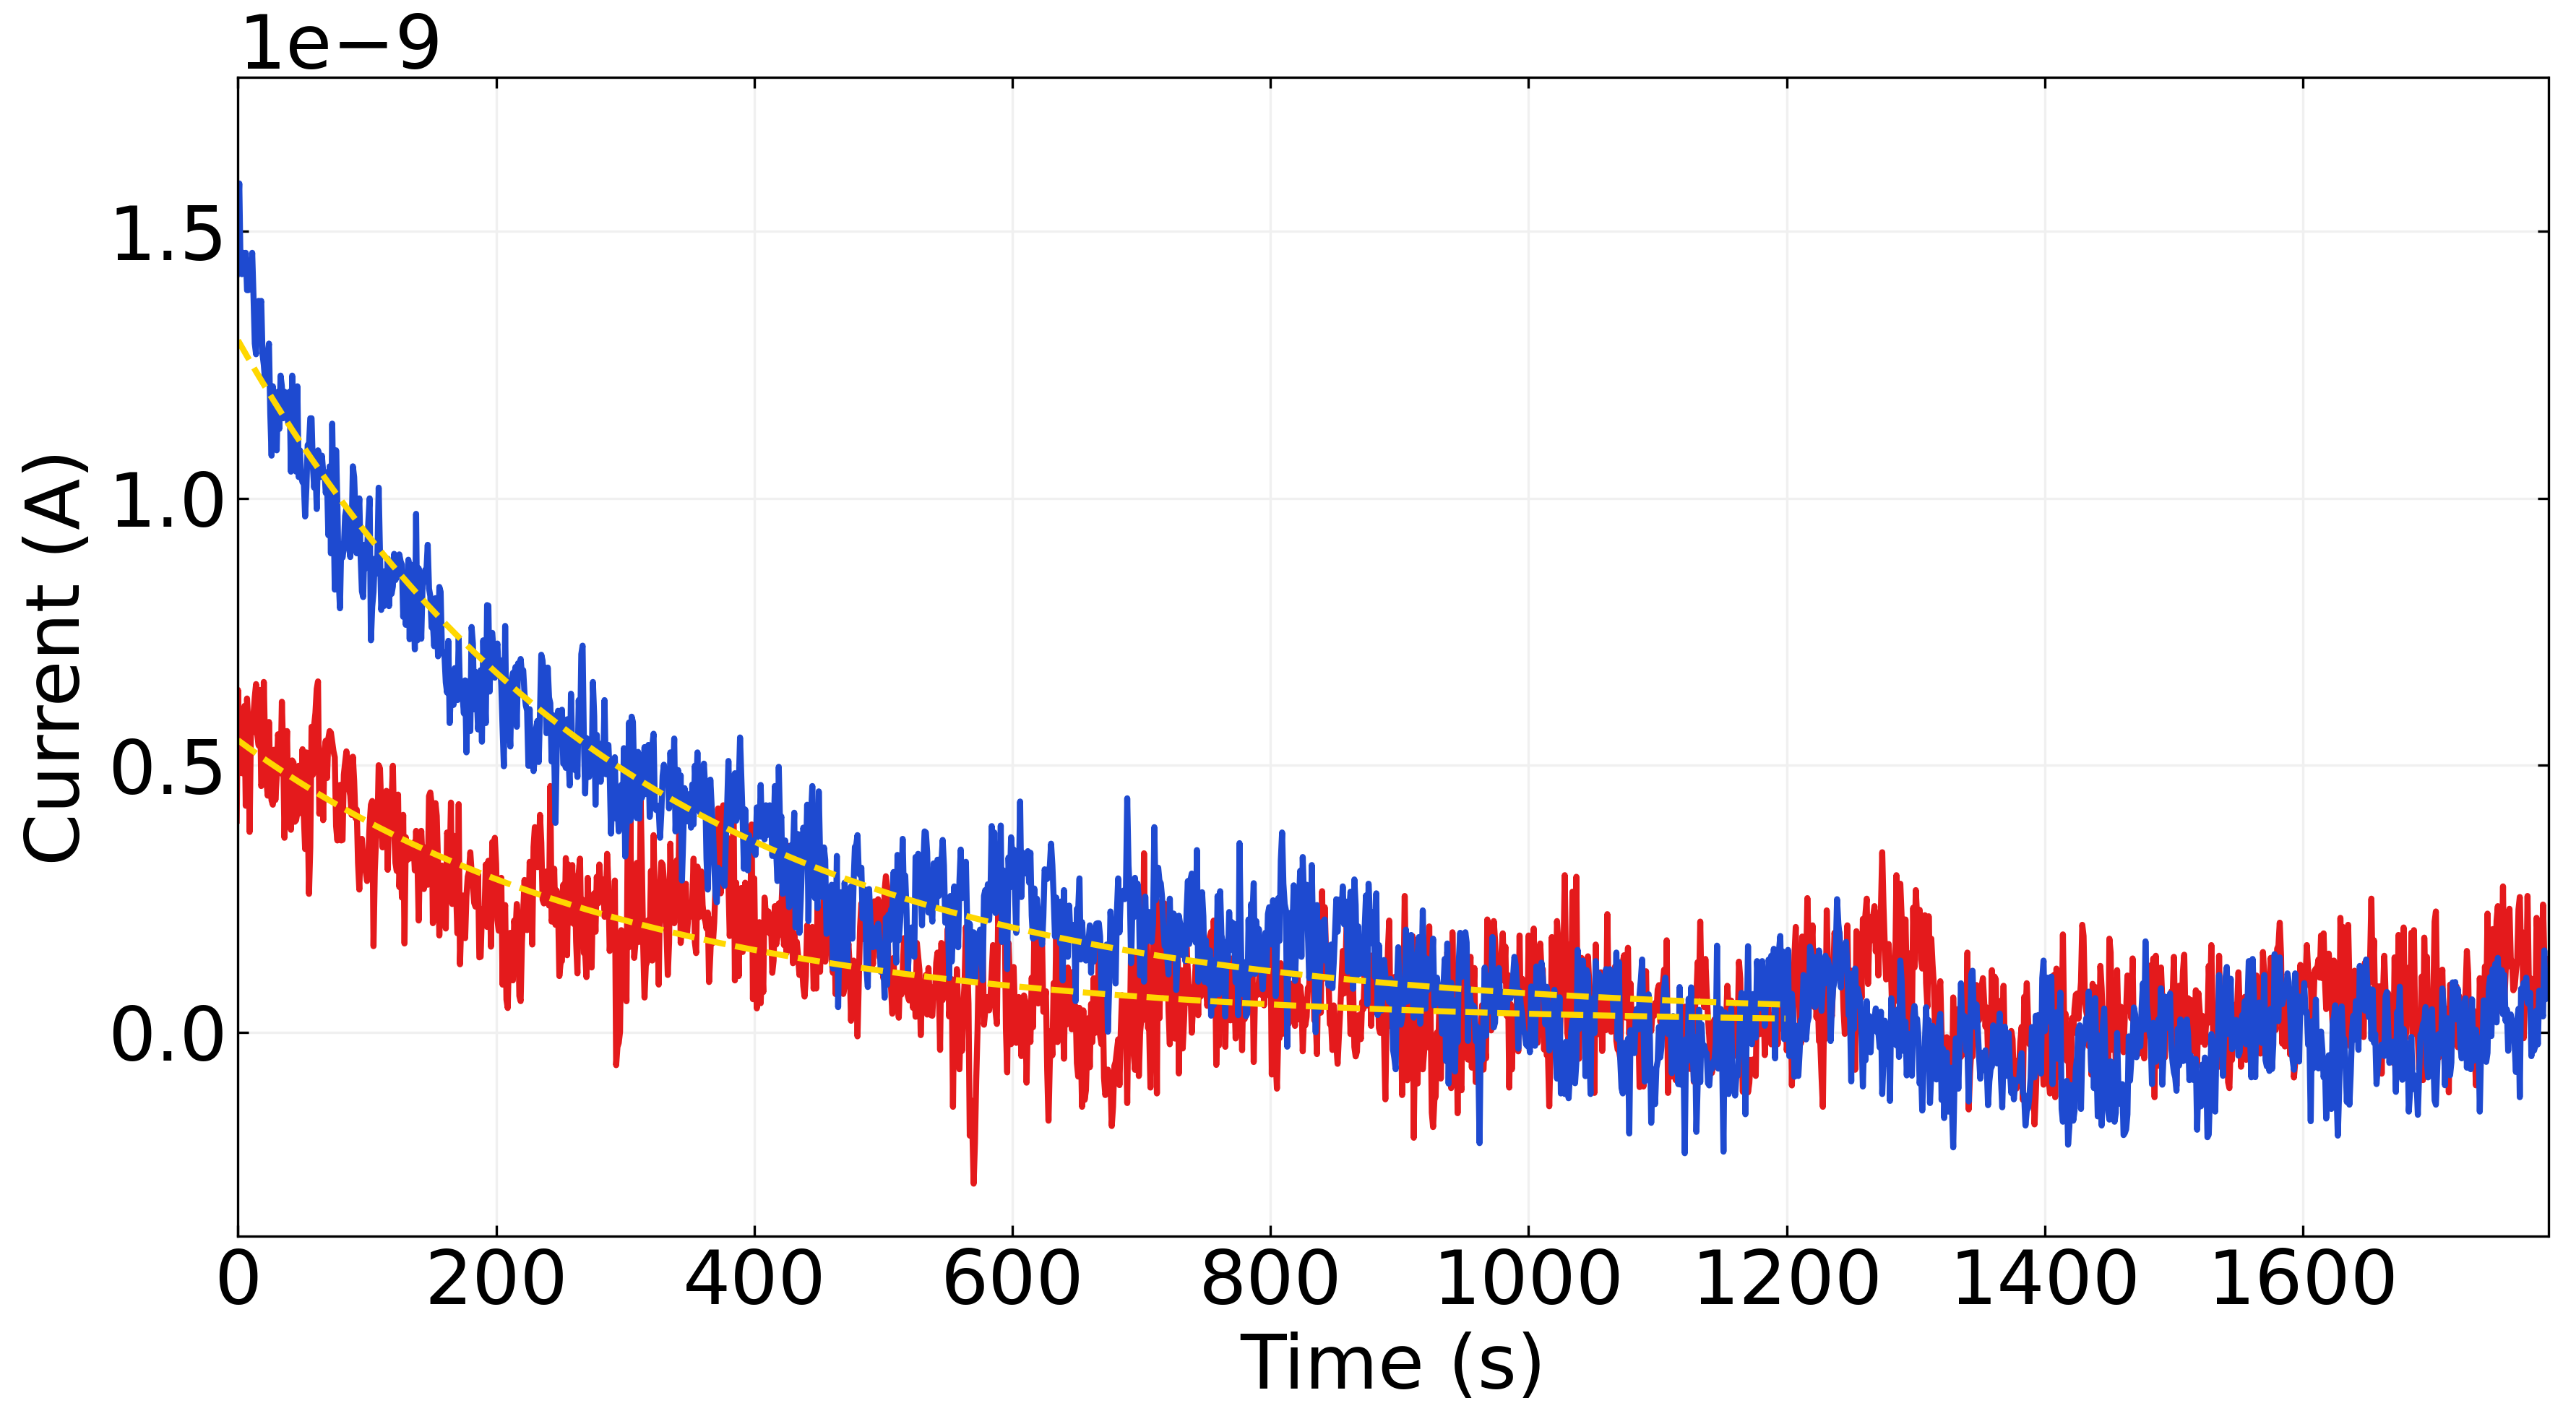
\includegraphics{figures/ch5/Q2C10_with_fitted_curves_exp.png}

}

}

\subcaption{\label{fig-exp-fit}}
\end{minipage}%
%
\begin{minipage}[t]{0.25\linewidth}

{\centering 

~

}

\end{minipage}%

\caption{\label{fig-salt-conc-control-series-SU8}The two gate voltages
used during the control series in (b) are marked on the transfer
characteristic in (a), where the transfer curve axis has been scaled so
as to be centered around the minimum of the reverse sweep. The linear
fits to the control series in (b) from 1200 s onwards had R squared
values of 0.78 and 0.70 for the traces with gate voltage
\(V_{\textrm{lg}}-V_{\textrm{gap}}\) = \(-200\) mV and
\(V_{\textrm{lg}}-V_{\textrm{gap}}\) = \(-150\) mV respectively. The
exponential fits in (c) from \(0-1200\) s had R squared values of 0.71
and 0.93 for the \(V_{\textrm{lg}}-V_{\textrm{gap}}\) = \(-200\) mV and
\(V_{\textrm{lg}}-V_{\textrm{gap}}\) = \(-150\) mV traces respectively.}

\end{figure}

Figure~\ref{fig-linear-fit} shows two control series performed using the
same channel on different days, with a different gate voltage used
during each series. In both series, there is no clear stepwise response
to any addition or subtraction of 1XPBS, as expected. We see that the
current has a period of rapid decay followed by slower baseline drift,
which has been observed previously for parallel arrangements of single
carbon nanotubes in air or vacuum \autocite{Lin2006,Noyce2019}. This
effect results from changes in the occupancy of charge traps in and
around the substrate and carbon nanotubes. The magnitude of baseline
drift is lower for our devices than for those characterised by Noyce
\emph{et al.}, which may be a result of numerous device and setup
differences which affect the presence of charge traps. These differences
include liquid-gating instead of back-gated, the use of a network of
carbon nanotubes instead of single nanotubes, a different channel
length, the use of a 300 nm instead of 90 nm SiO\(_2\) layer, and the
use of an asymmetric, liquid-gated transfer sweep over a shorter voltage
range to characterise devices before each control series was measured
\autocite{Noyce2019}.

As a first approximation to the longer time constant exponentials
discussed by Noyce \emph{et al.}, linear fits were performed on each
control series from \(1200-1800\) s. The gradient of the
\(V_{\textrm{lg}}-V_{\textrm{gap}}\) = \(-200\) mV gated control series
was \(m_{1} = -0.95\pm0.02\) pA/s, while the gradient of the
\(V_{\textrm{lg}}-V_{\textrm{gap}}\) = \(-150\) mV gated control series
was \(m_{2} = -0.69\pm0.02\) pA/s. The equations for the two linear fits
were proportional to each other, with
\(m_{2}t + b_{2} = (0.73 \pm 0.03)\times (m_{1}t + b_{1})\). This
indicates a relationship between the voltage used to gate the devices
and the degree of longer-term baseline drift. This effect is likely a
consequence of gate bias stress, where gating introduces charge traps to
the channel over time and reduces drain current. The more negative the
applied bias, the larger the amplitude of the longer-term drift
\autocite{Bargaoui2018}.

When the longer-term linear fits were subtracted from the raw data, the
remaining dataset followed a exponential decay trend for both control
series. Figure~\ref{fig-exp-fit} shows exponential fits to the remaining
curve from \(0-1200\) s. Both exponentials had a characteristic time
constant of \(\tau = 300 \pm 20\) s, indicating this rate of decay is
independent of the gate voltage used to gate the transistor. They are
therefore also proportional to each other, with
\(a_{2}\exp(-t/\tau) = (2.39\pm0.05)\times a_{1}\exp(-t/\tau)\). The
\(V_{\textrm{lg}}-V_{\textrm{gap}}\) = \(-200\) mV measurement was
performed 3 days after the \(V_{\textrm{lg}}-V_{\textrm{gap}}\) =
\(-150\) mV measurement. It seems that the amplitude of the exponential
term is history dependent and reduced with each subsequent control
series. This behaviour is unlike that of the devices characterised by
Noyce \emph{et al.}, where the amplitude of the initial decay
exponential remained the same after a initial reset gate sweep. It
therefore appears that the sweep performed on these devices before
measurement is insufficient to redistribute charges in trap states and
reset the baseline drift, which could be a consequence of being
liquid-gated instead of back-gated, being asymmetric or being over a
shorter voltage range \autocite{Noyce2019}.

\begin{figure}

\begin{minipage}[t]{0.40\linewidth}

{\centering 

\raisebox{-\height}{

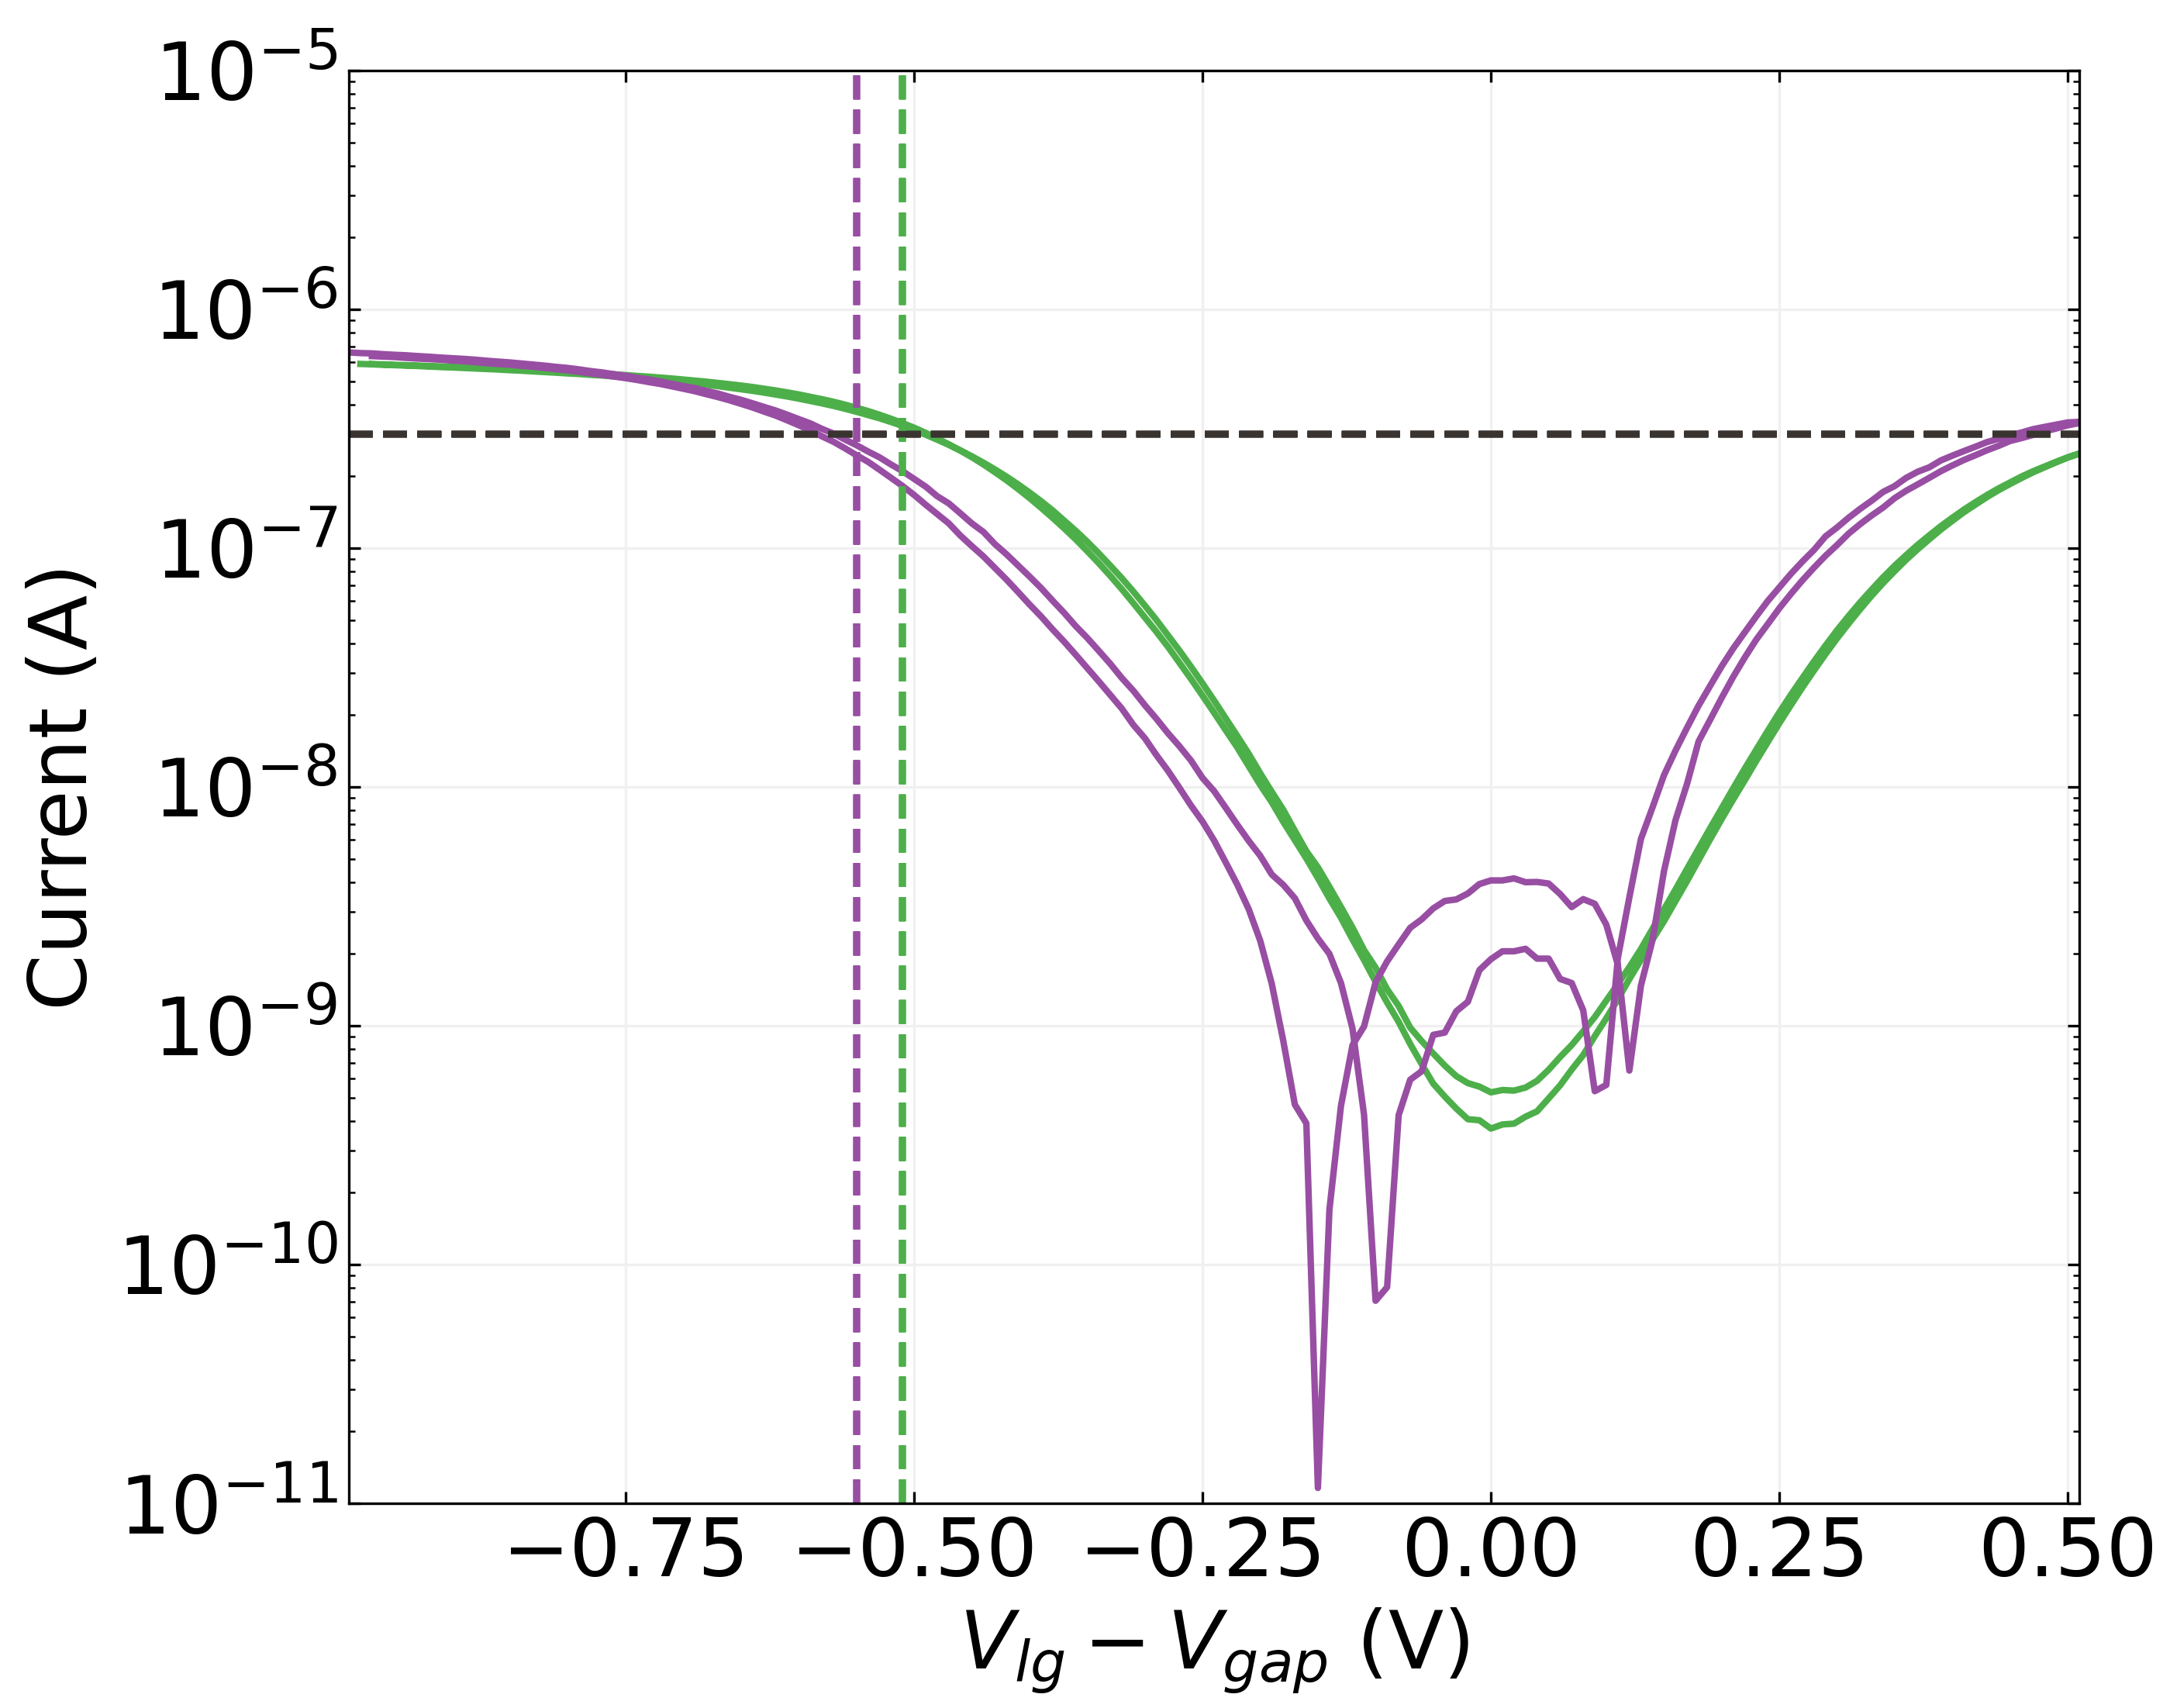
\includegraphics{figures/ch5/Q31C1_absolute_values_without_gate_current.png}

}

}

\subcaption{\label{fig-transfer-sweep-AZ1518}}
\end{minipage}%
%
\begin{minipage}[t]{0.05\linewidth}

{\centering 

~

}

\end{minipage}%
%
\begin{minipage}[t]{0.55\linewidth}

{\centering 

\raisebox{-\height}{

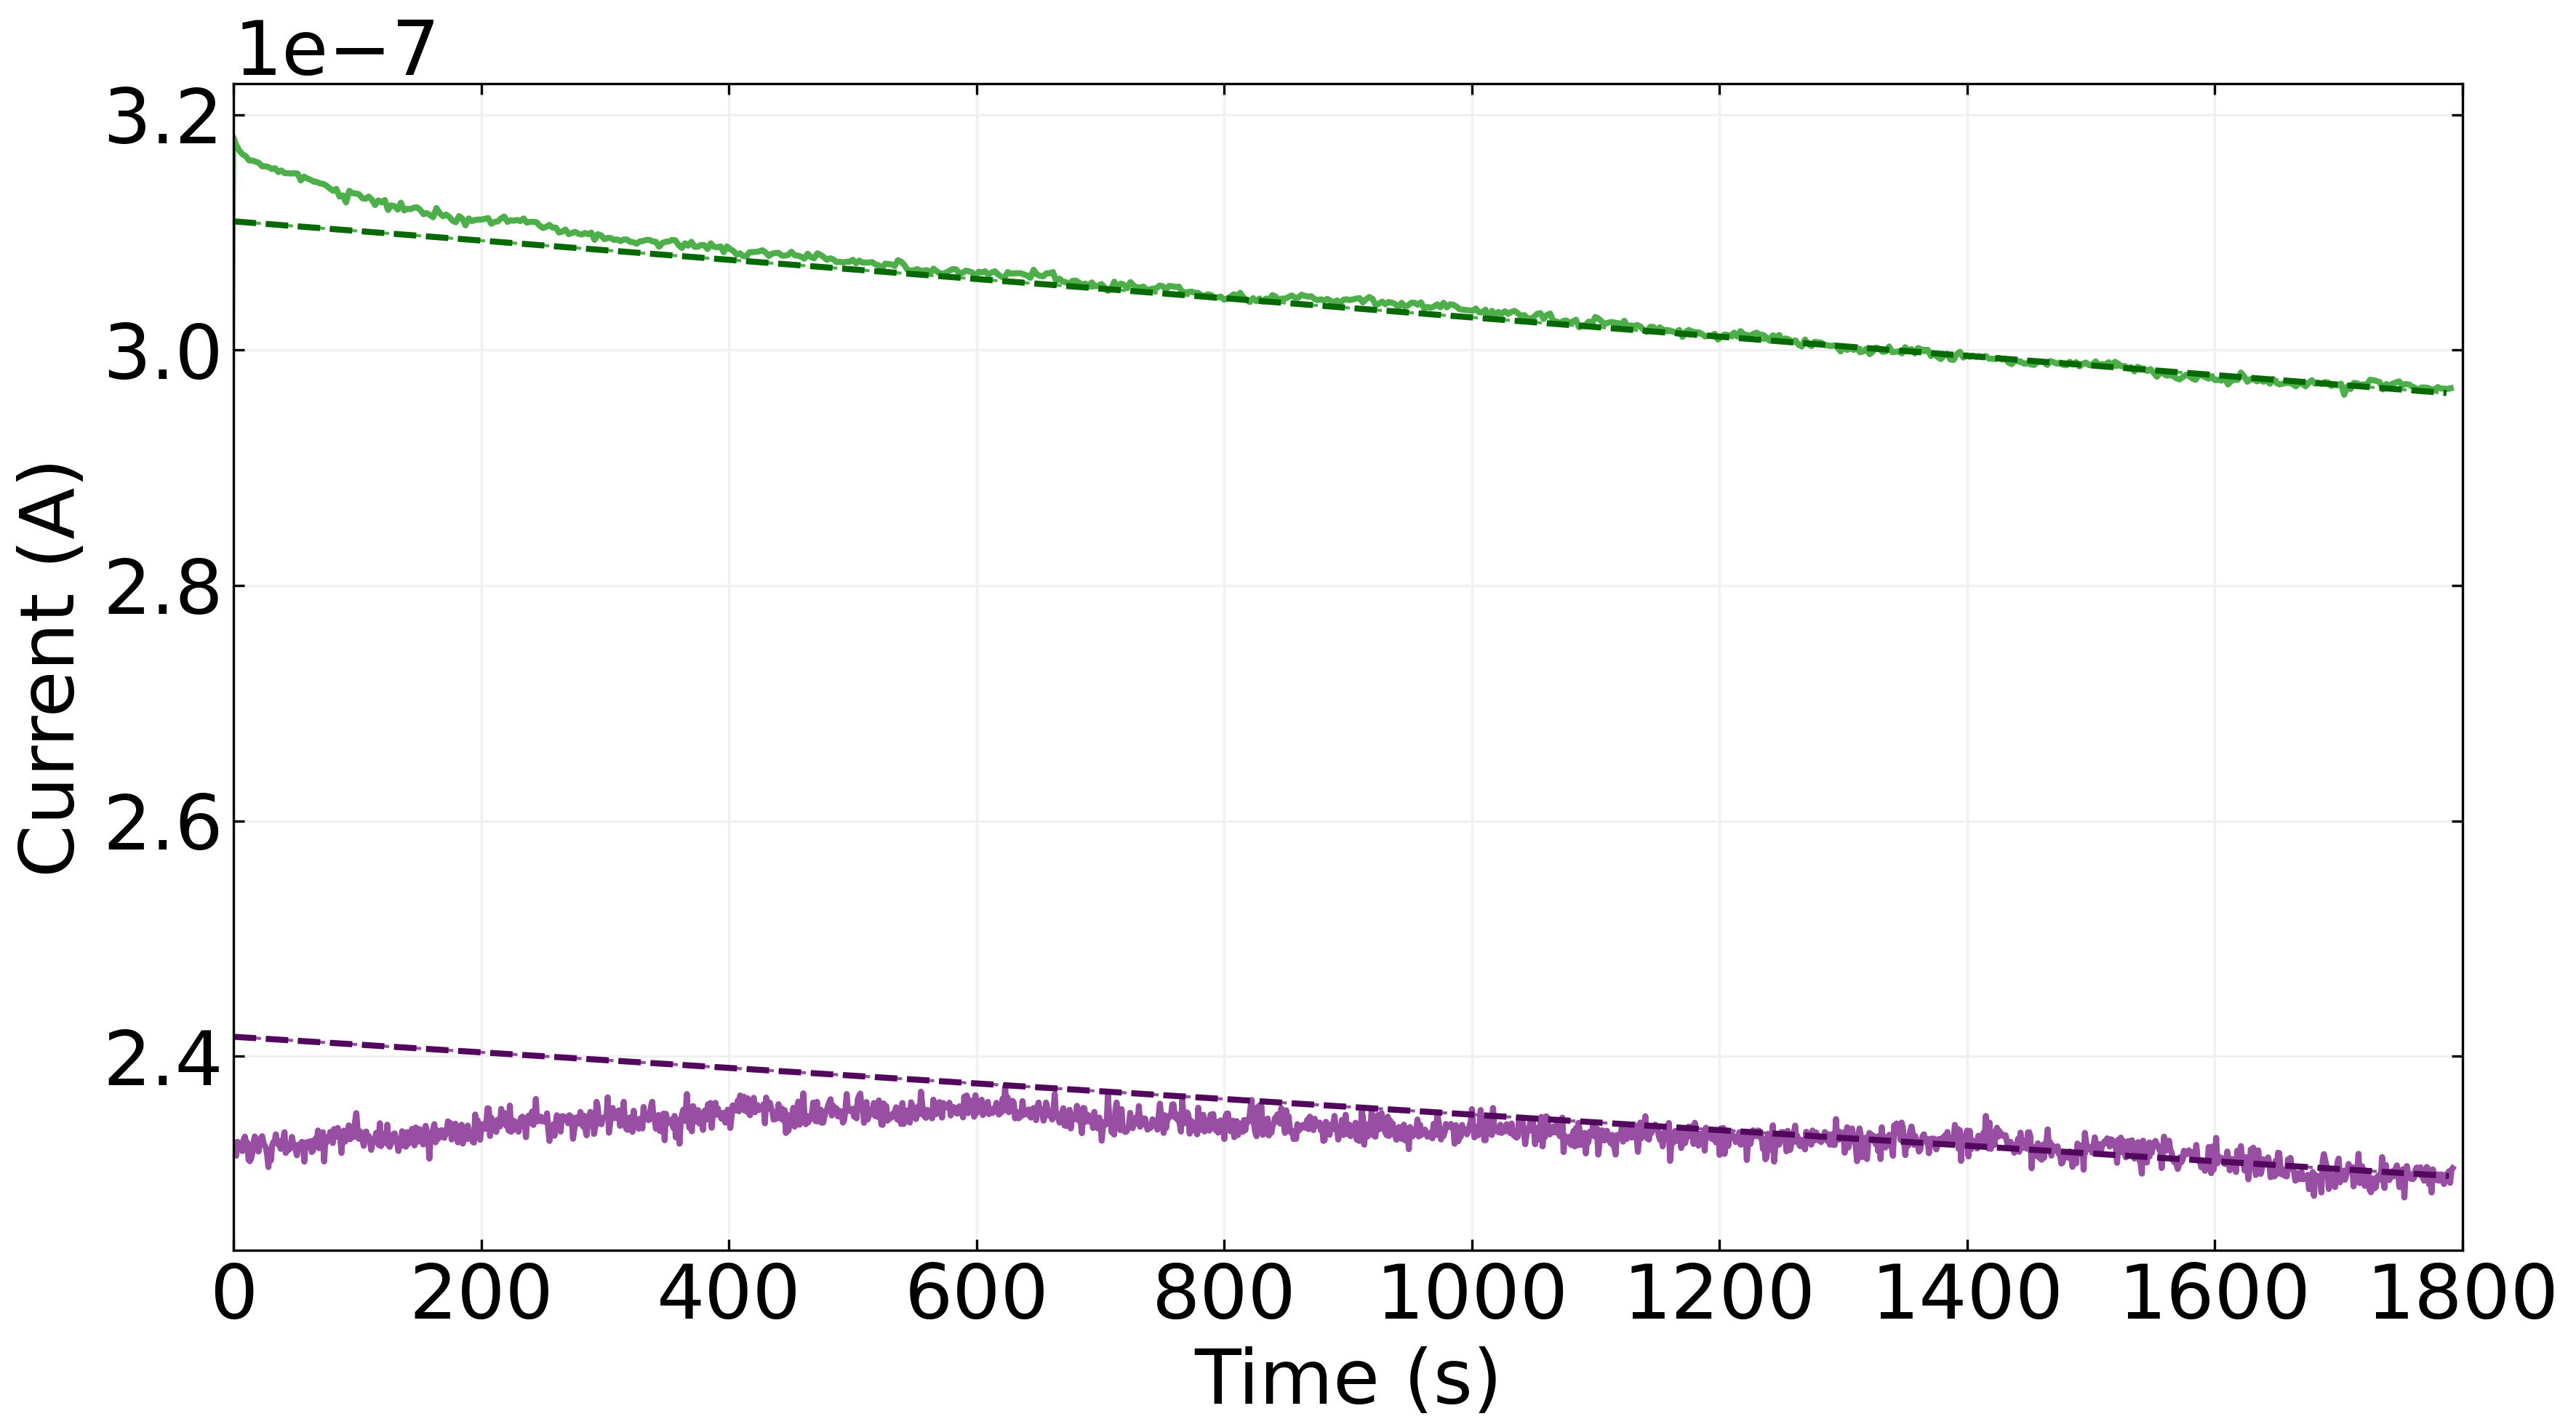
\includegraphics{figures/ch5/Q31C1_with_fitted_curves.png}

}

}

\subcaption{\label{fig-linear-fit-AZ1518}}
\end{minipage}%
\newline
\begin{minipage}[t]{0.23\linewidth}

{\centering 

~

}

\end{minipage}%
%
\begin{minipage}[t]{0.55\linewidth}

{\centering 

\raisebox{-\height}{

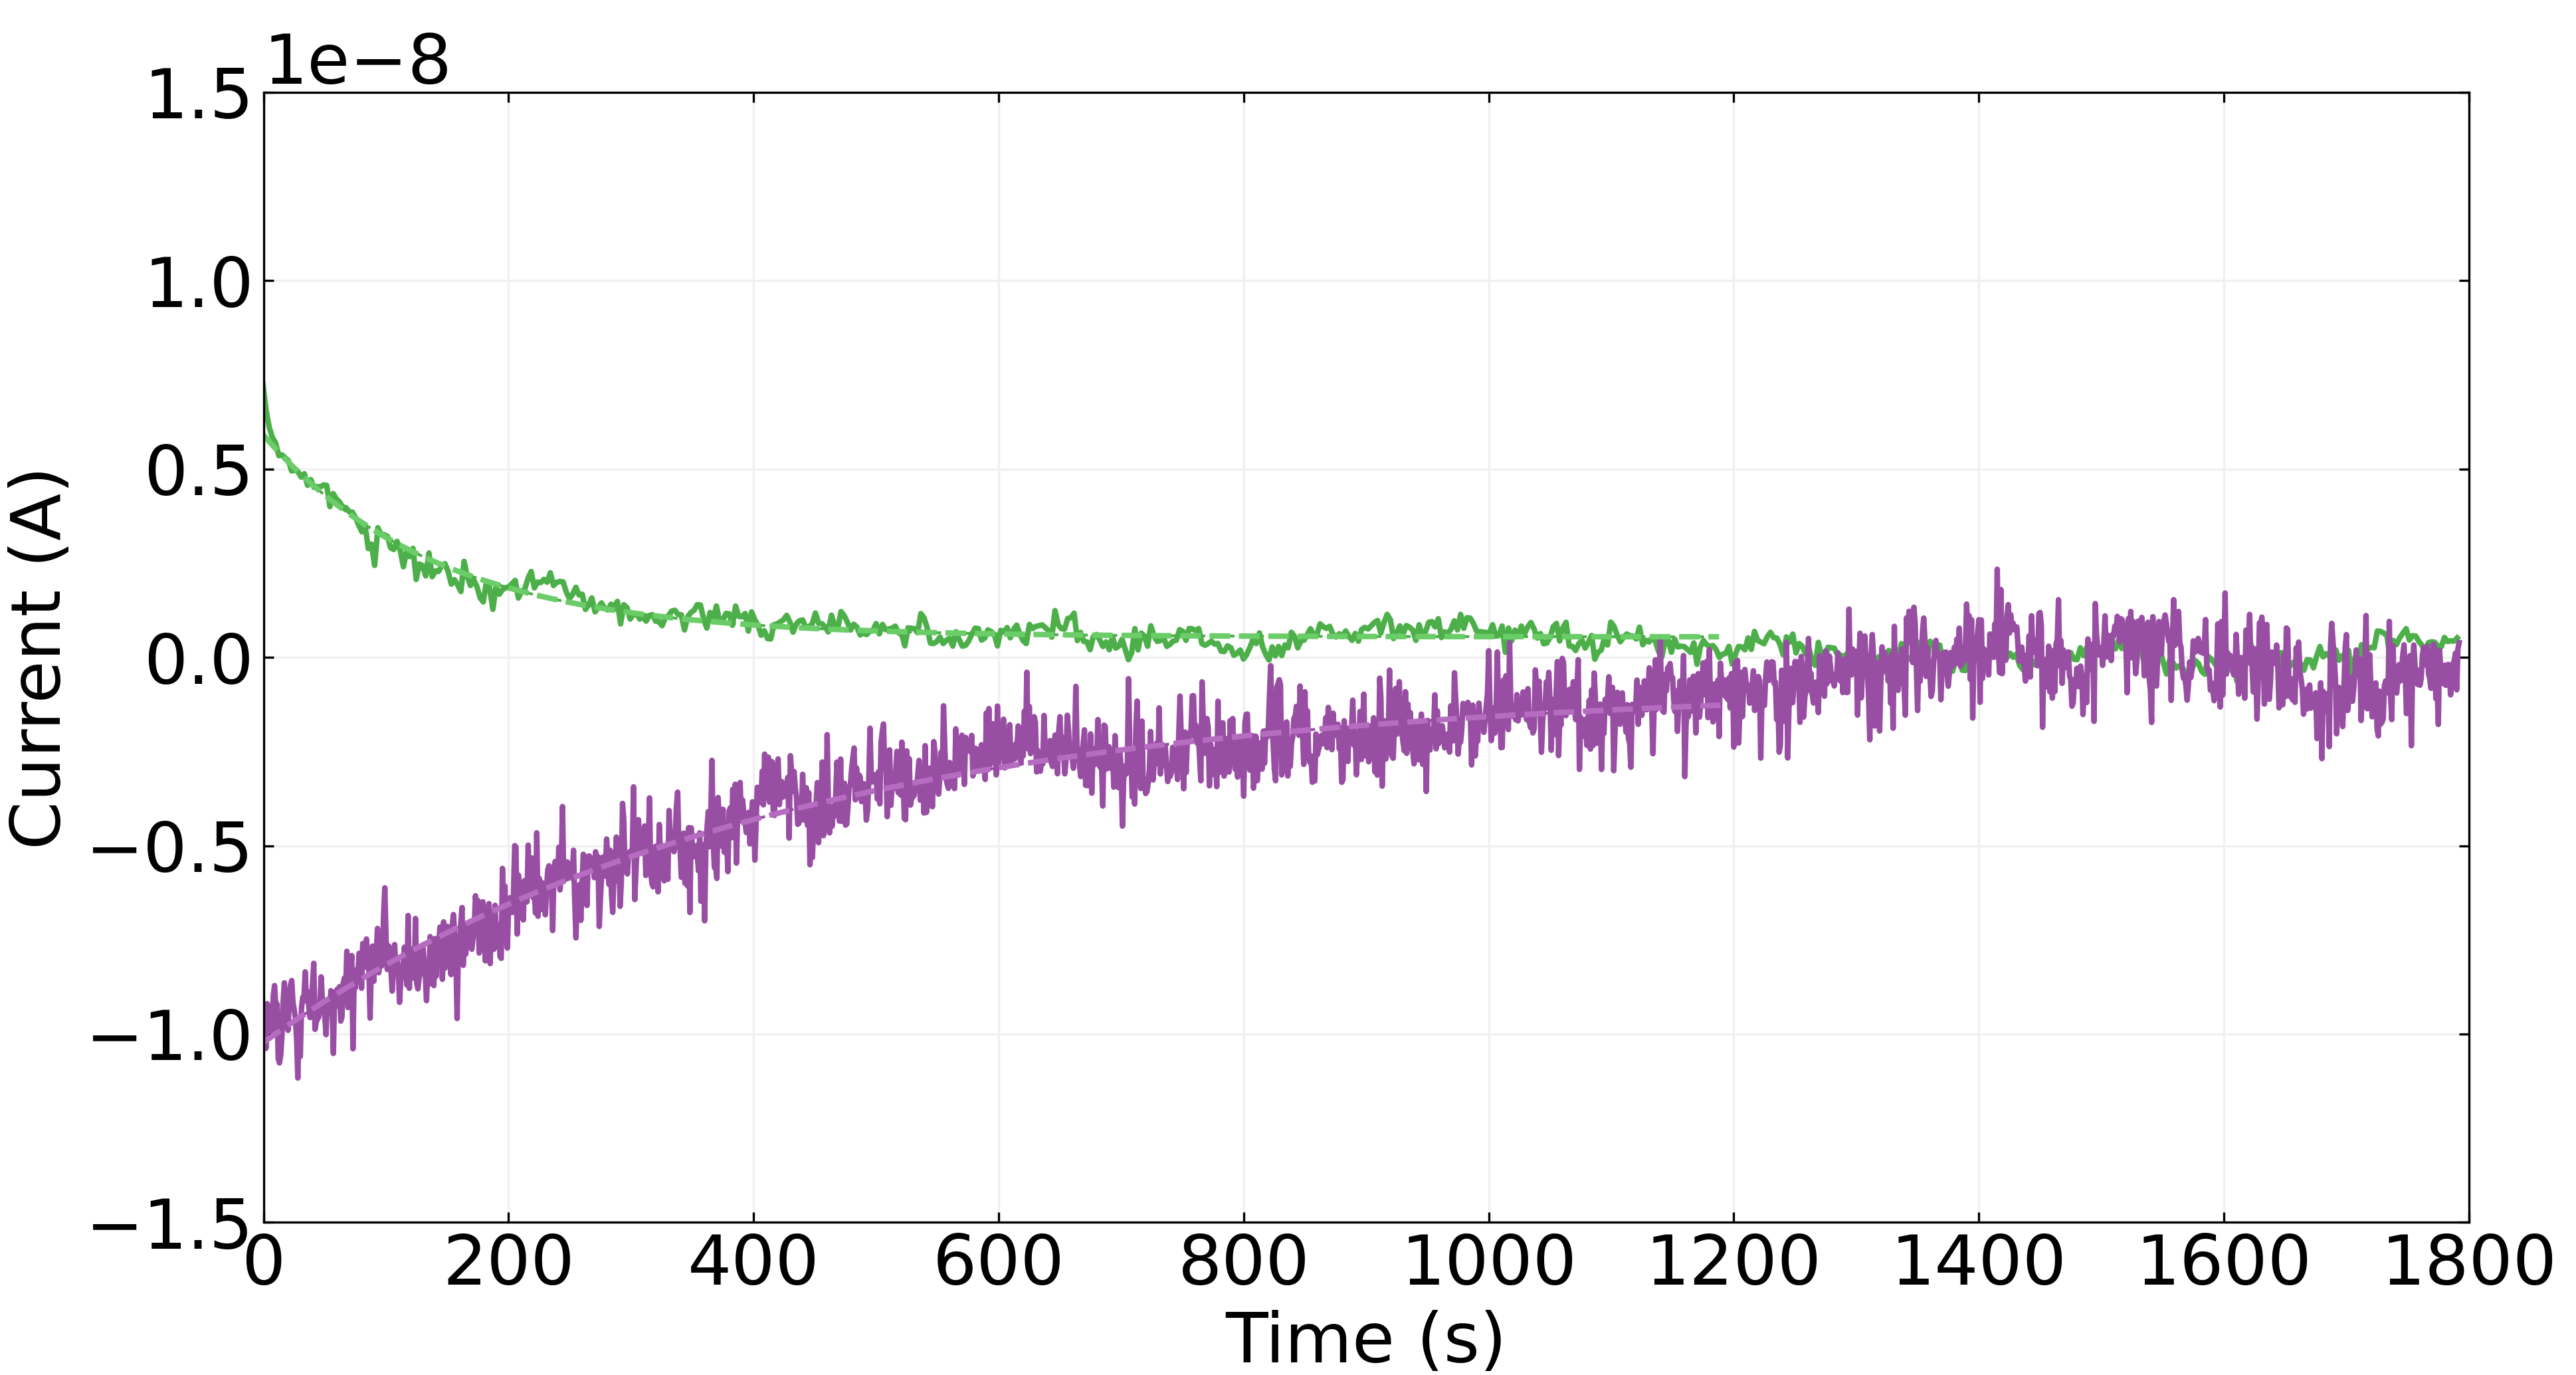
\includegraphics{figures/ch5/Q31C1_with_fitted_curves_exp.png}

}

}

\subcaption{\label{fig-exp-fit-AZ1518}}
\end{minipage}%
%
\begin{minipage}[t]{0.23\linewidth}

{\centering 

~

}

\end{minipage}%

\caption{\label{fig-salt-conc-control-series-AZ1518}The absolute-value
transfer characteristics for the channels from Device 1 and Device 2
used in the control series in (b) are shown in (a), coloured green and
purple respectively. The transfer curve axis has been scaled so as to be
centered around the minimum of the reverse sweep, or in the case of
Device 2, the centre point between the voltages where current drops to
zero in the reverse sweep. The gate voltages used for each device during
the control series in (b) are marked on the transfer characteristics in
(a) in the same colour as their corresponding device. The linear fits to
the control series in (b) from 1200 s onwards had R squared values of
0.96 and 0.67, and the exponential fits in (c) from \(0-1200\) s had R
squared values of 0.94 and 0.92 for Devices 1 \& 2 respectively.}

\end{figure}

Figure~\ref{fig-transfer-sweep-AZ1518} shows channel transfer
characteristics from two different steam-assisted surfactant-deposited,
AZ\(^\circledR\) 1518 encapsulated devices fabricated in different
device batches. The central feature in the transfer characteristic in
device 2 represents absolute-value measurements of `negative current'.
These are unphysical measurements which come from equipment error and
can be treated as zero current passing through the channel, and
therefore V\(_{\textrm{gap}}\) is located in the center of this region.
Device 1, with the channel characteristic curve shown in green, was
fabricated in Mar 2023. Device 2, with the channel characteristic curve
shown in purple, was fabricated after Jun 2023. Device 2 was flood
exposed, rinsed with AZ\(^\circledR\) 326 developer and annealed at
\(150^\circ\)C before measurement. When taking control series
measurements, the devices were gated so that the current level for each
control series would be as similar as possible, as illustrated by the
dotted lines in Figure~\ref{fig-transfer-sweep-AZ1518}.

As in Figure~\ref{fig-linear-fit}, linear fits were performed on each
control series from \(1200-1800\) s, shown in
Figure~\ref{fig-linear-fit-AZ1518}. The gradient of the control series
corresponding to Device 1 was \(m_{1} = -8.2\pm0.1\) pA/s, while the
gradient of the control series corresponding to Device 2 was
\(m_{2} = -6.6\pm0.2\). Again, the equations for the two linear fits
were proportional to each other, where
\(m_{2}t + b_{2} = (0.81 \pm 0.03)\times (m_{1}t + b_{1})\), despite
being different channels from a different device batch. This result
indicates that gate bias stress has the same effect on baseline drift on
channels of different devices fabricated in the same manner.

As with the SU8 device, subtracting the linear fit resulted in a a
dataset which followed an exponential trend.
Figure~\ref{fig-exp-fit-AZ1518} shows exponential fits from \(0-1200\) s
to the remaining curves from the AZ\(^\circledR\) 1518 devices. The time
constants for these exponentials were dissimilar, with a time constant
of \(\tau = 141 \pm 3\) s for Device 1 and a time constant of
\(\tau = 408 \pm 11\) s for Device 2. The exponential amplitudes had
opposite sign, with the first indicating an increase in net positive
trapped charge and the latter indicating an increase in net negative
trapped charge. It appears the difference in processing between the
devices has changed the net charge of the traps initially present when
measuring the control series.

From this analysis it appears that the baseline drift for the
liquid-gated carbon nanotube devices can be accurately approximated as a
combination of a exponential and linear term. The linear term appears to
be consistent across channels of a particular device type, with the size
of this term increasing with increasingly negative gate bias. The time
constant of the exponential term appears to be intrinsic to the channel
being measured.

\hypertarget{sec-salt-conc-series}{%
\subsection{Sensing Series}\label{sec-salt-conc-series}}

A salt concentration sensing series were performed from 1800 s onwards,
directly after the control series. Salt concentration testing was done
to confirm the fabricated devices were sensitive to small environmental
changes in their pristine state, to check for spurious signals, and to
ensure gate current leakage or other confounding factors were not
contributing to sensing responses. The PDMS well contained 80 \(\mu\)L
1X PBS at 1800 s. During the series, successive additions of deionised
water were made to reduce the concentration of PBS in the well. An
initial 1X PBS addition was performed at 2100s, to confirm no changes
occurred during the control series that would interfere with sensing.
All additions to the well in the sensing series and resulting changes to
the PBS concentration in the well are shown in
Table~\ref{tbl-salt-conc-series}.

\hypertarget{tbl-salt-conc-series}{}
\begin{table}
\caption{\label{tbl-salt-conc-series}This table shows the times at which 20 µL additions were made to the
PDMS well, with 300 s between each addition. The concentration in the
well after each addition and the change in concentration after each
addition are also shown. The well contained 80 µL of 1X PBS at 1800 s. }\tabularnewline

\centering
\begin{tabular}{lcccccc}
\toprule
\multicolumn{1}{c}{ } & \multicolumn{1}{c}{1X PBS Addition} & \multicolumn{5}{c}{DI Water Additions} \\
\cmidrule(l{3pt}r{3pt}){2-2} \cmidrule(l{3pt}r{3pt}){3-7}
Time (s) & 2100 & 2400 & 2700 & 3000 & 3300 & 3600\\
Final PBS volume (µL) & 100 & 120 & 140 & 160 & 180 & 200\\
Final PBS concentration & 1X & 0.83X & 0.71X & 0.63X & 0.56X & 0.50X\\
Δ PBS concentration & 0 & -0.17X & -0.12X & -0.09X & -0.07X & -0.06X\\
\bottomrule
\end{tabular}
\end{table}

\begin{figure}

\begin{minipage}[t]{0.50\linewidth}

{\centering 

\raisebox{-\height}{

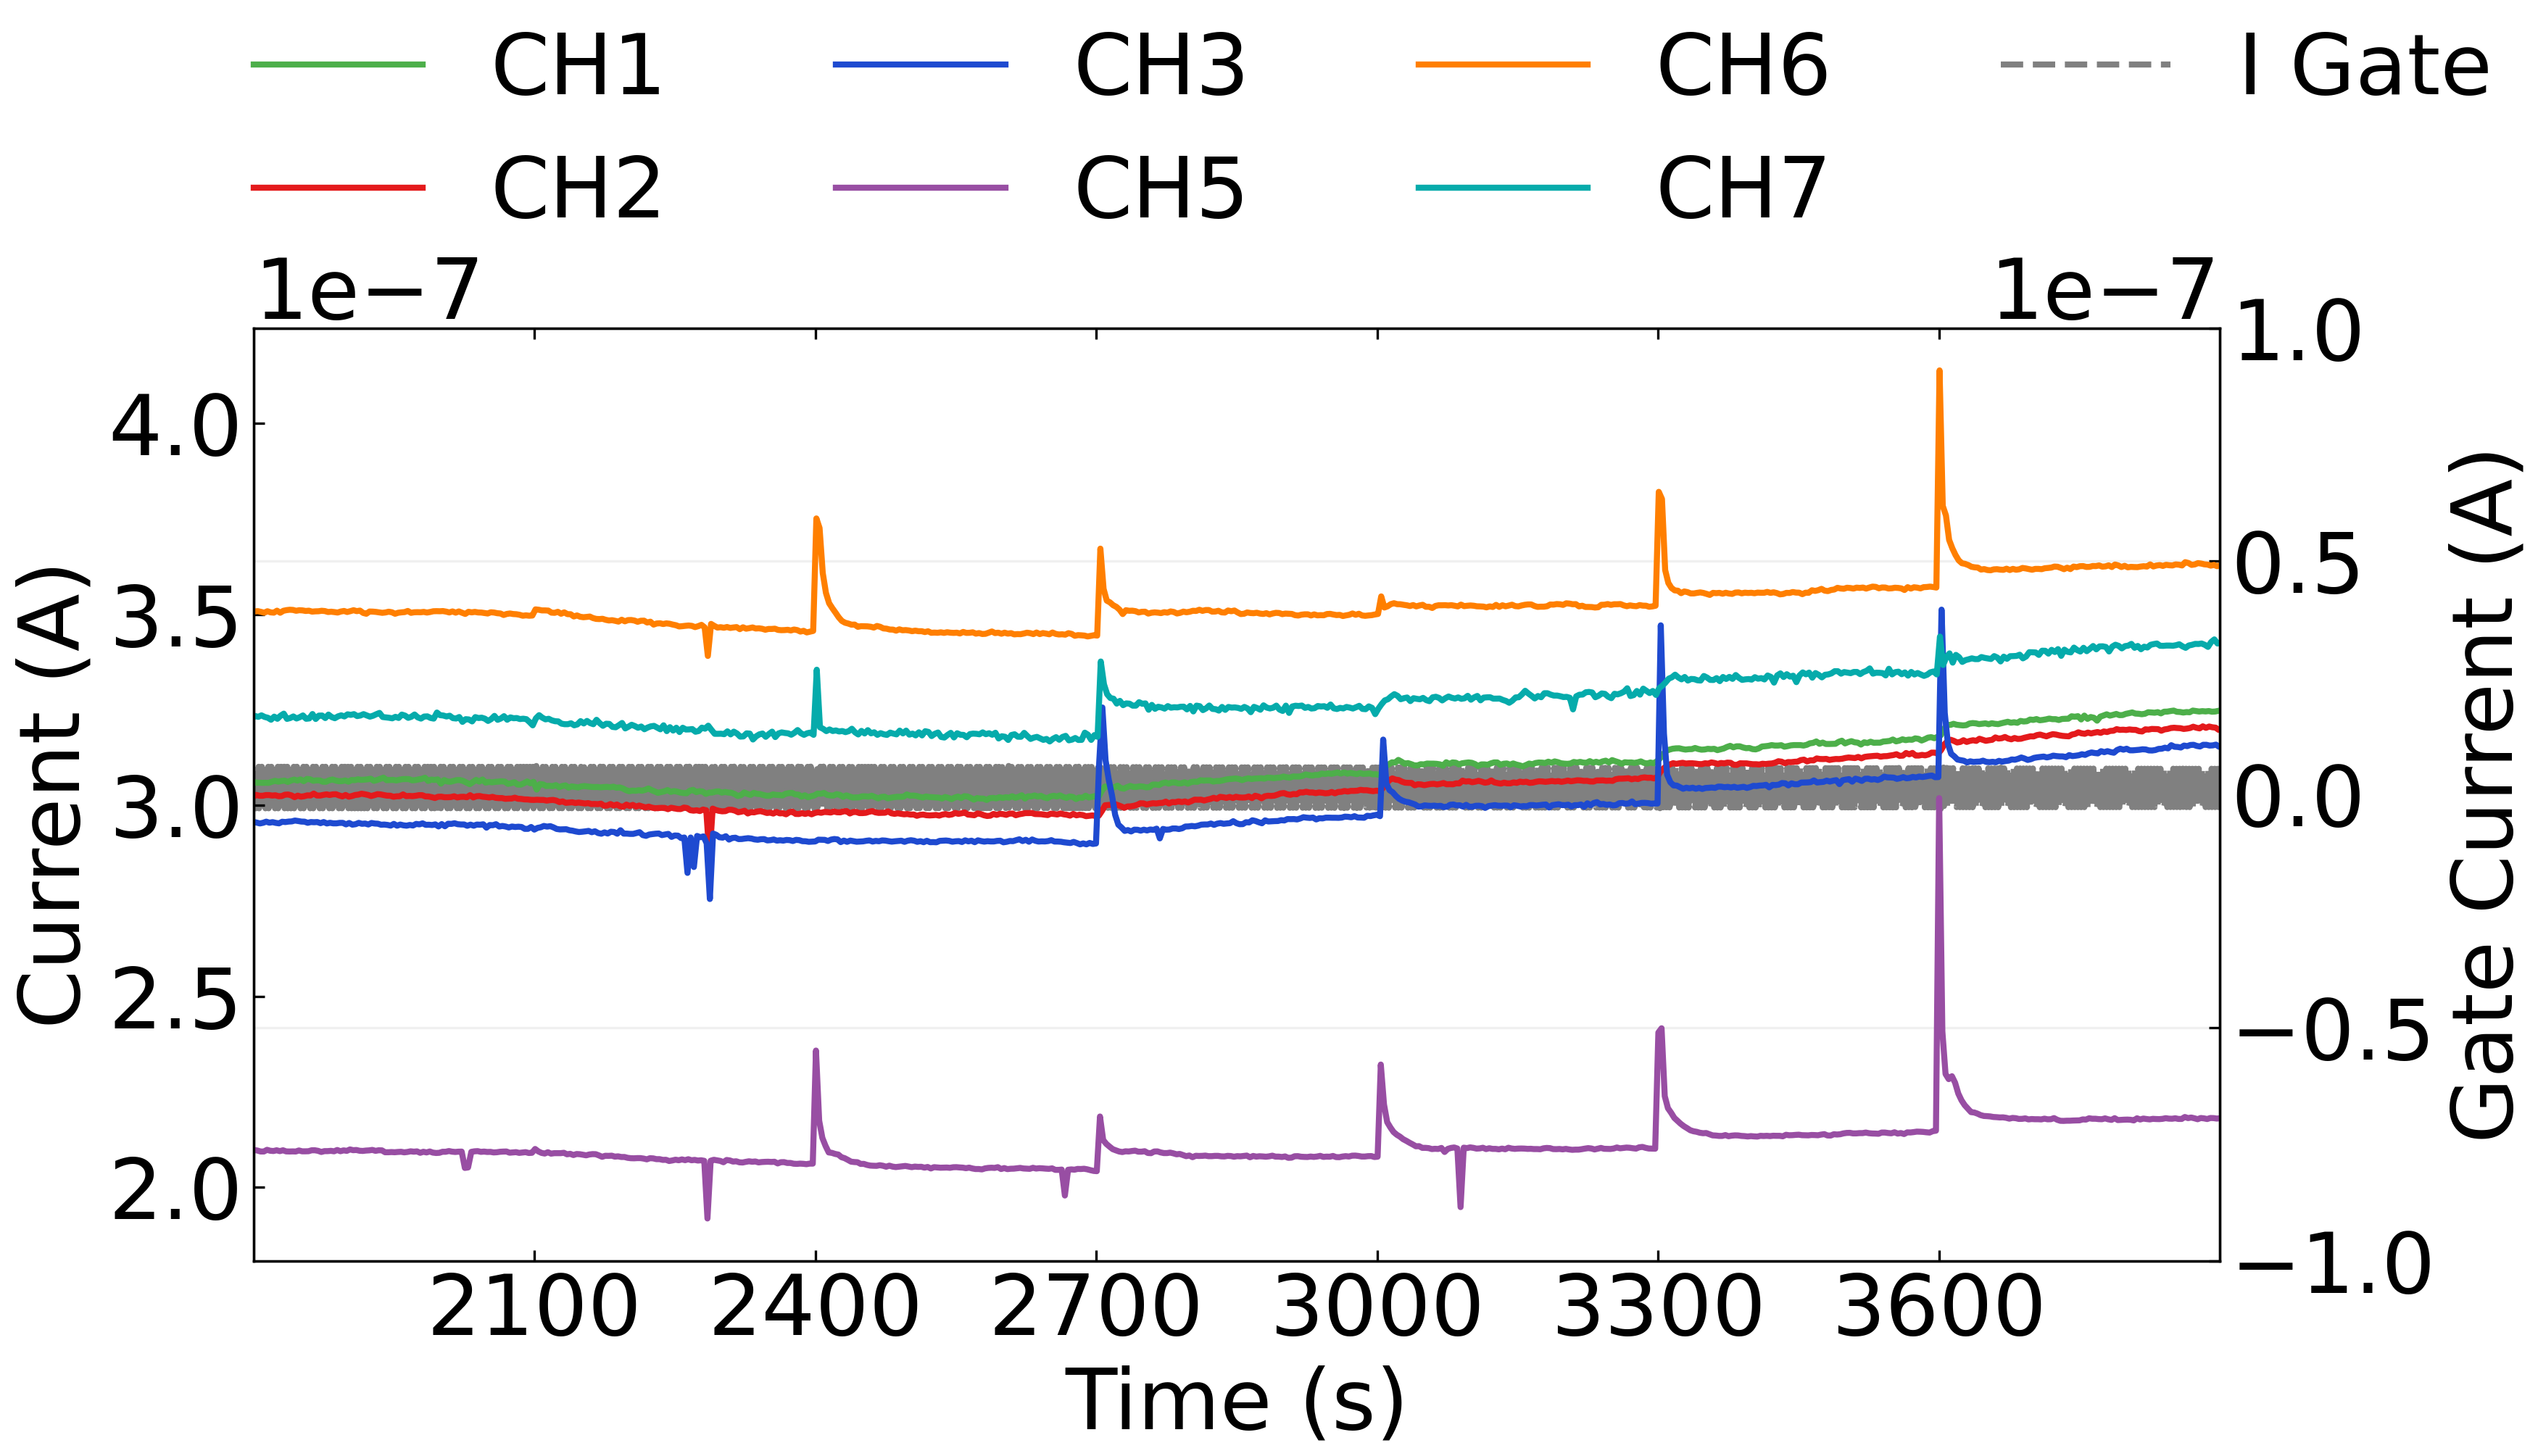
\includegraphics{figures/ch5/NTQ31C1_pristine_saltconc_sample_230324.png}

}

}

\subcaption{\label{fig-salt-conc-no-norm}}
\end{minipage}%
%
\begin{minipage}[t]{0.50\linewidth}

{\centering 

\raisebox{-\height}{

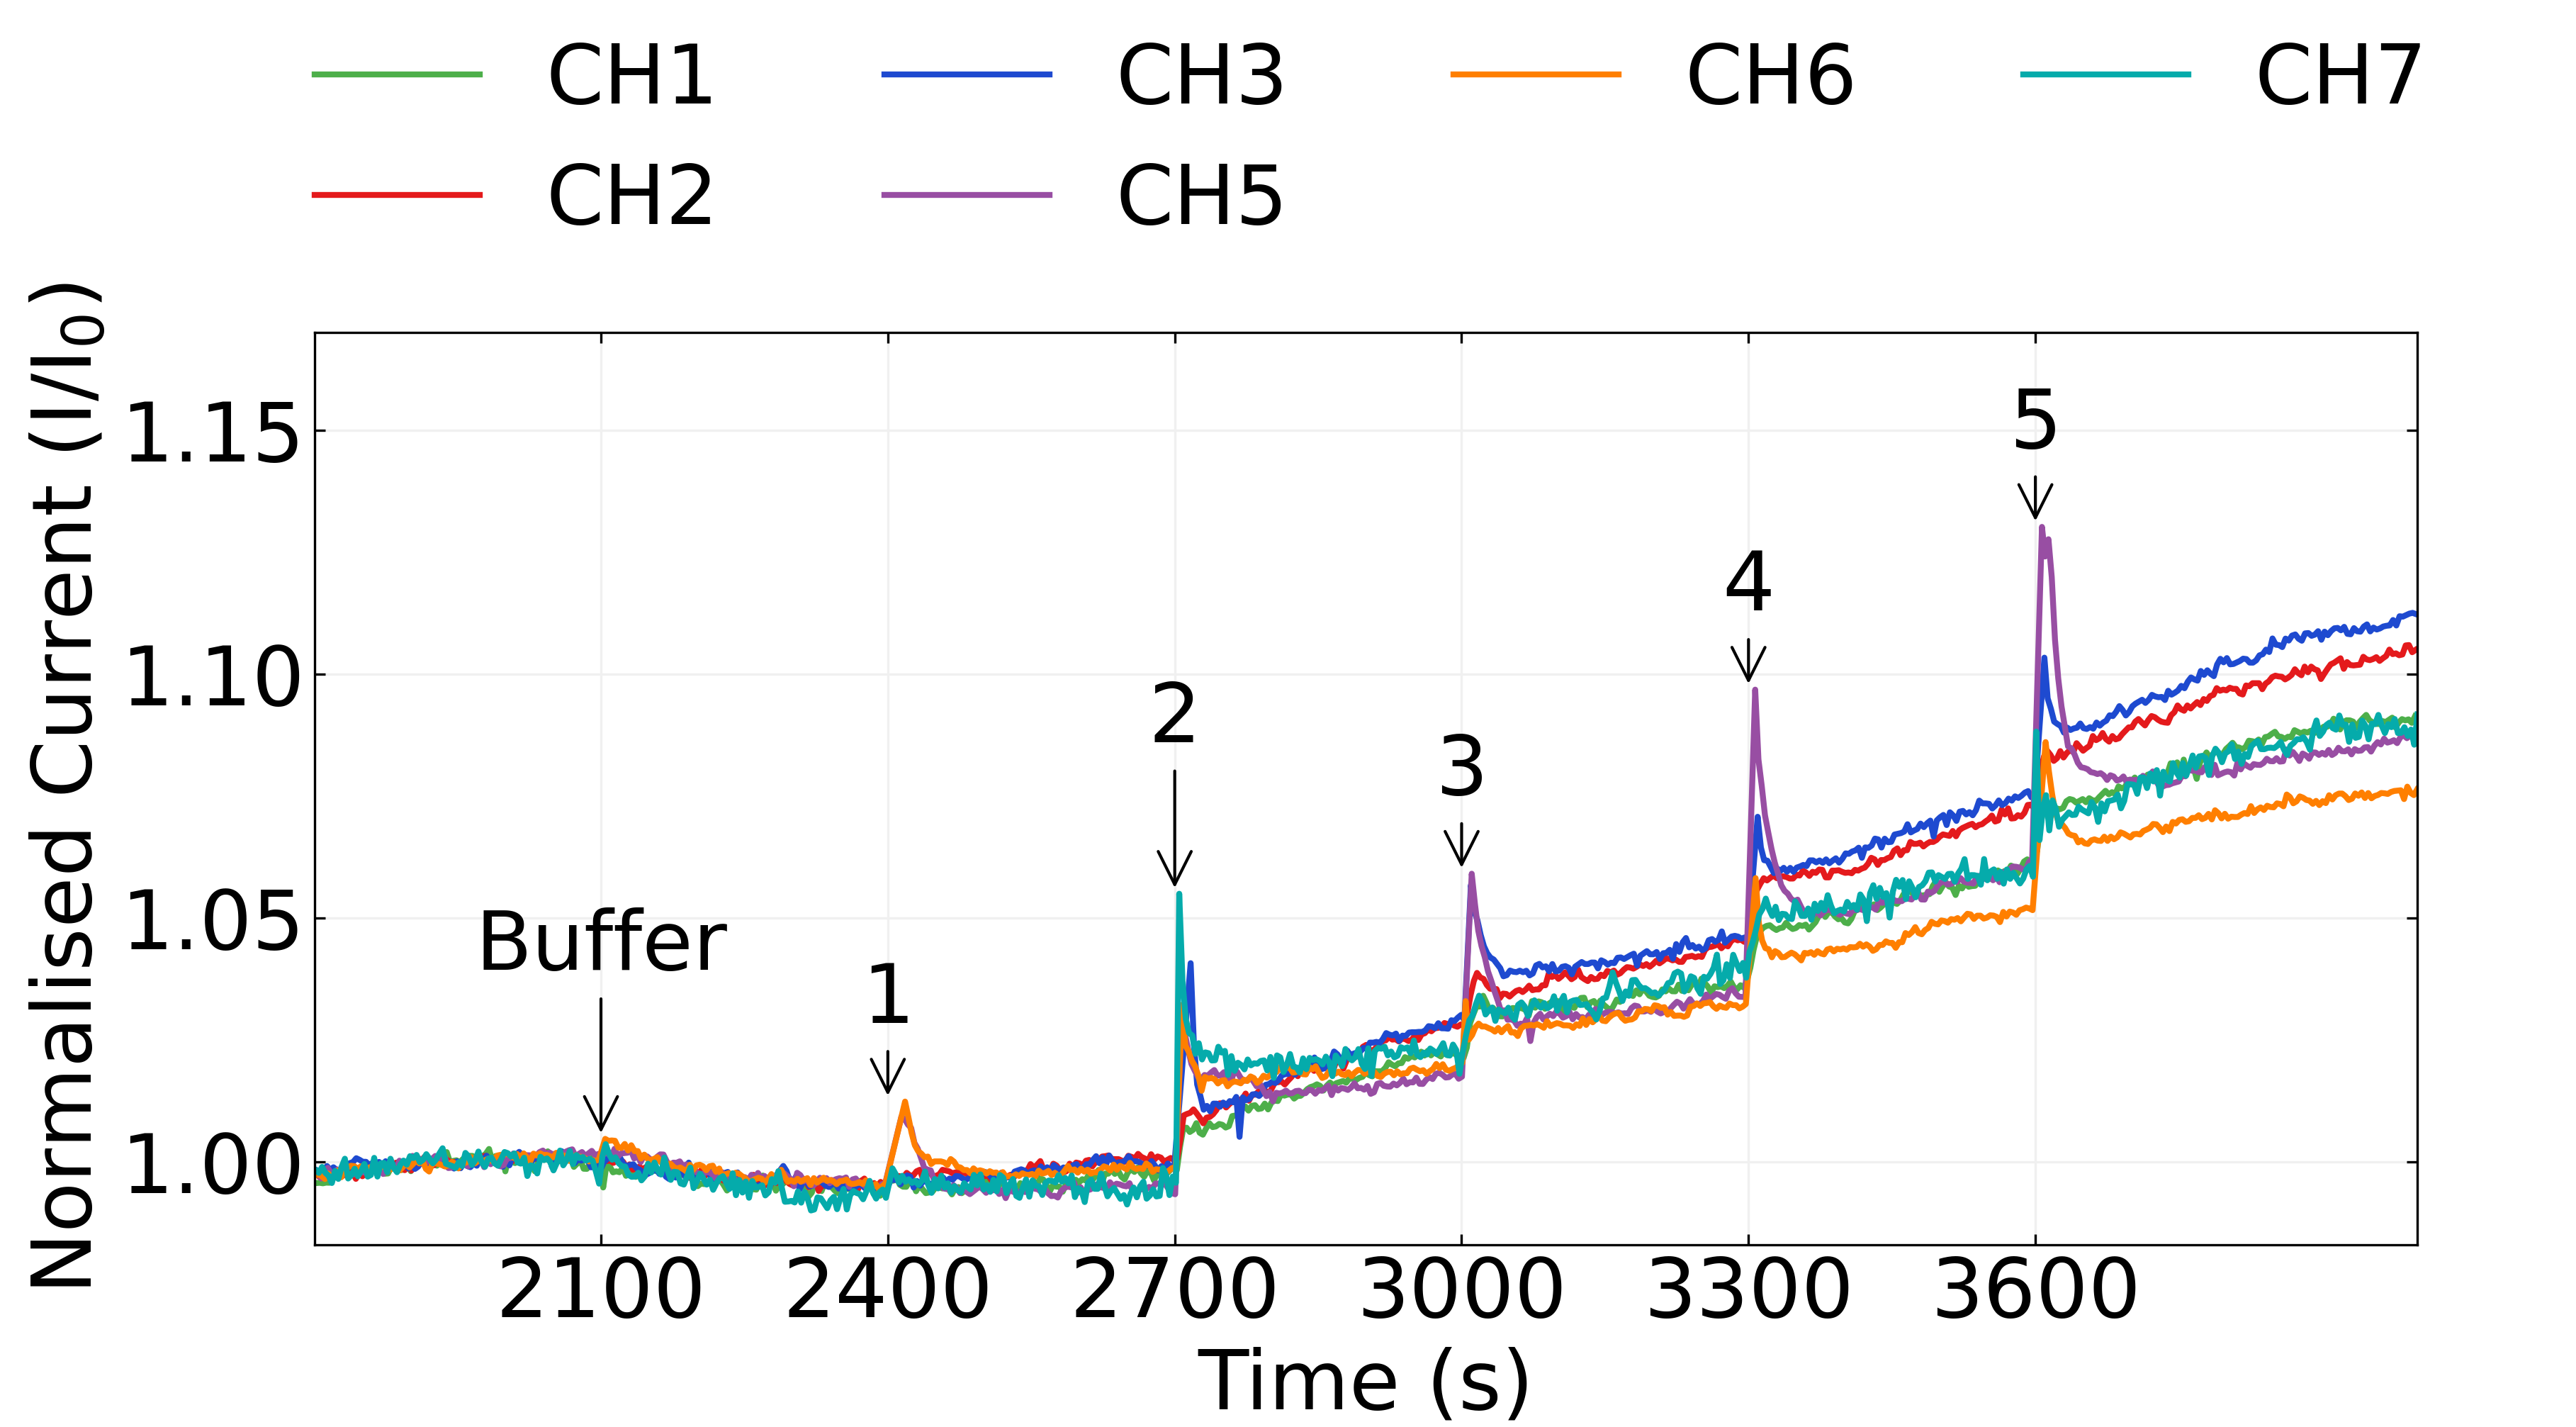
\includegraphics{figures/ch5/NTQ31C1_pristine_saltconc_sample_230324_detrend_trunc_arrows_normalised.png}

}

}

\subcaption{\label{fig-salt-conc-detrend}}
\end{minipage}%
\newline
\begin{minipage}[t]{0.50\linewidth}

{\centering 

\raisebox{-\height}{

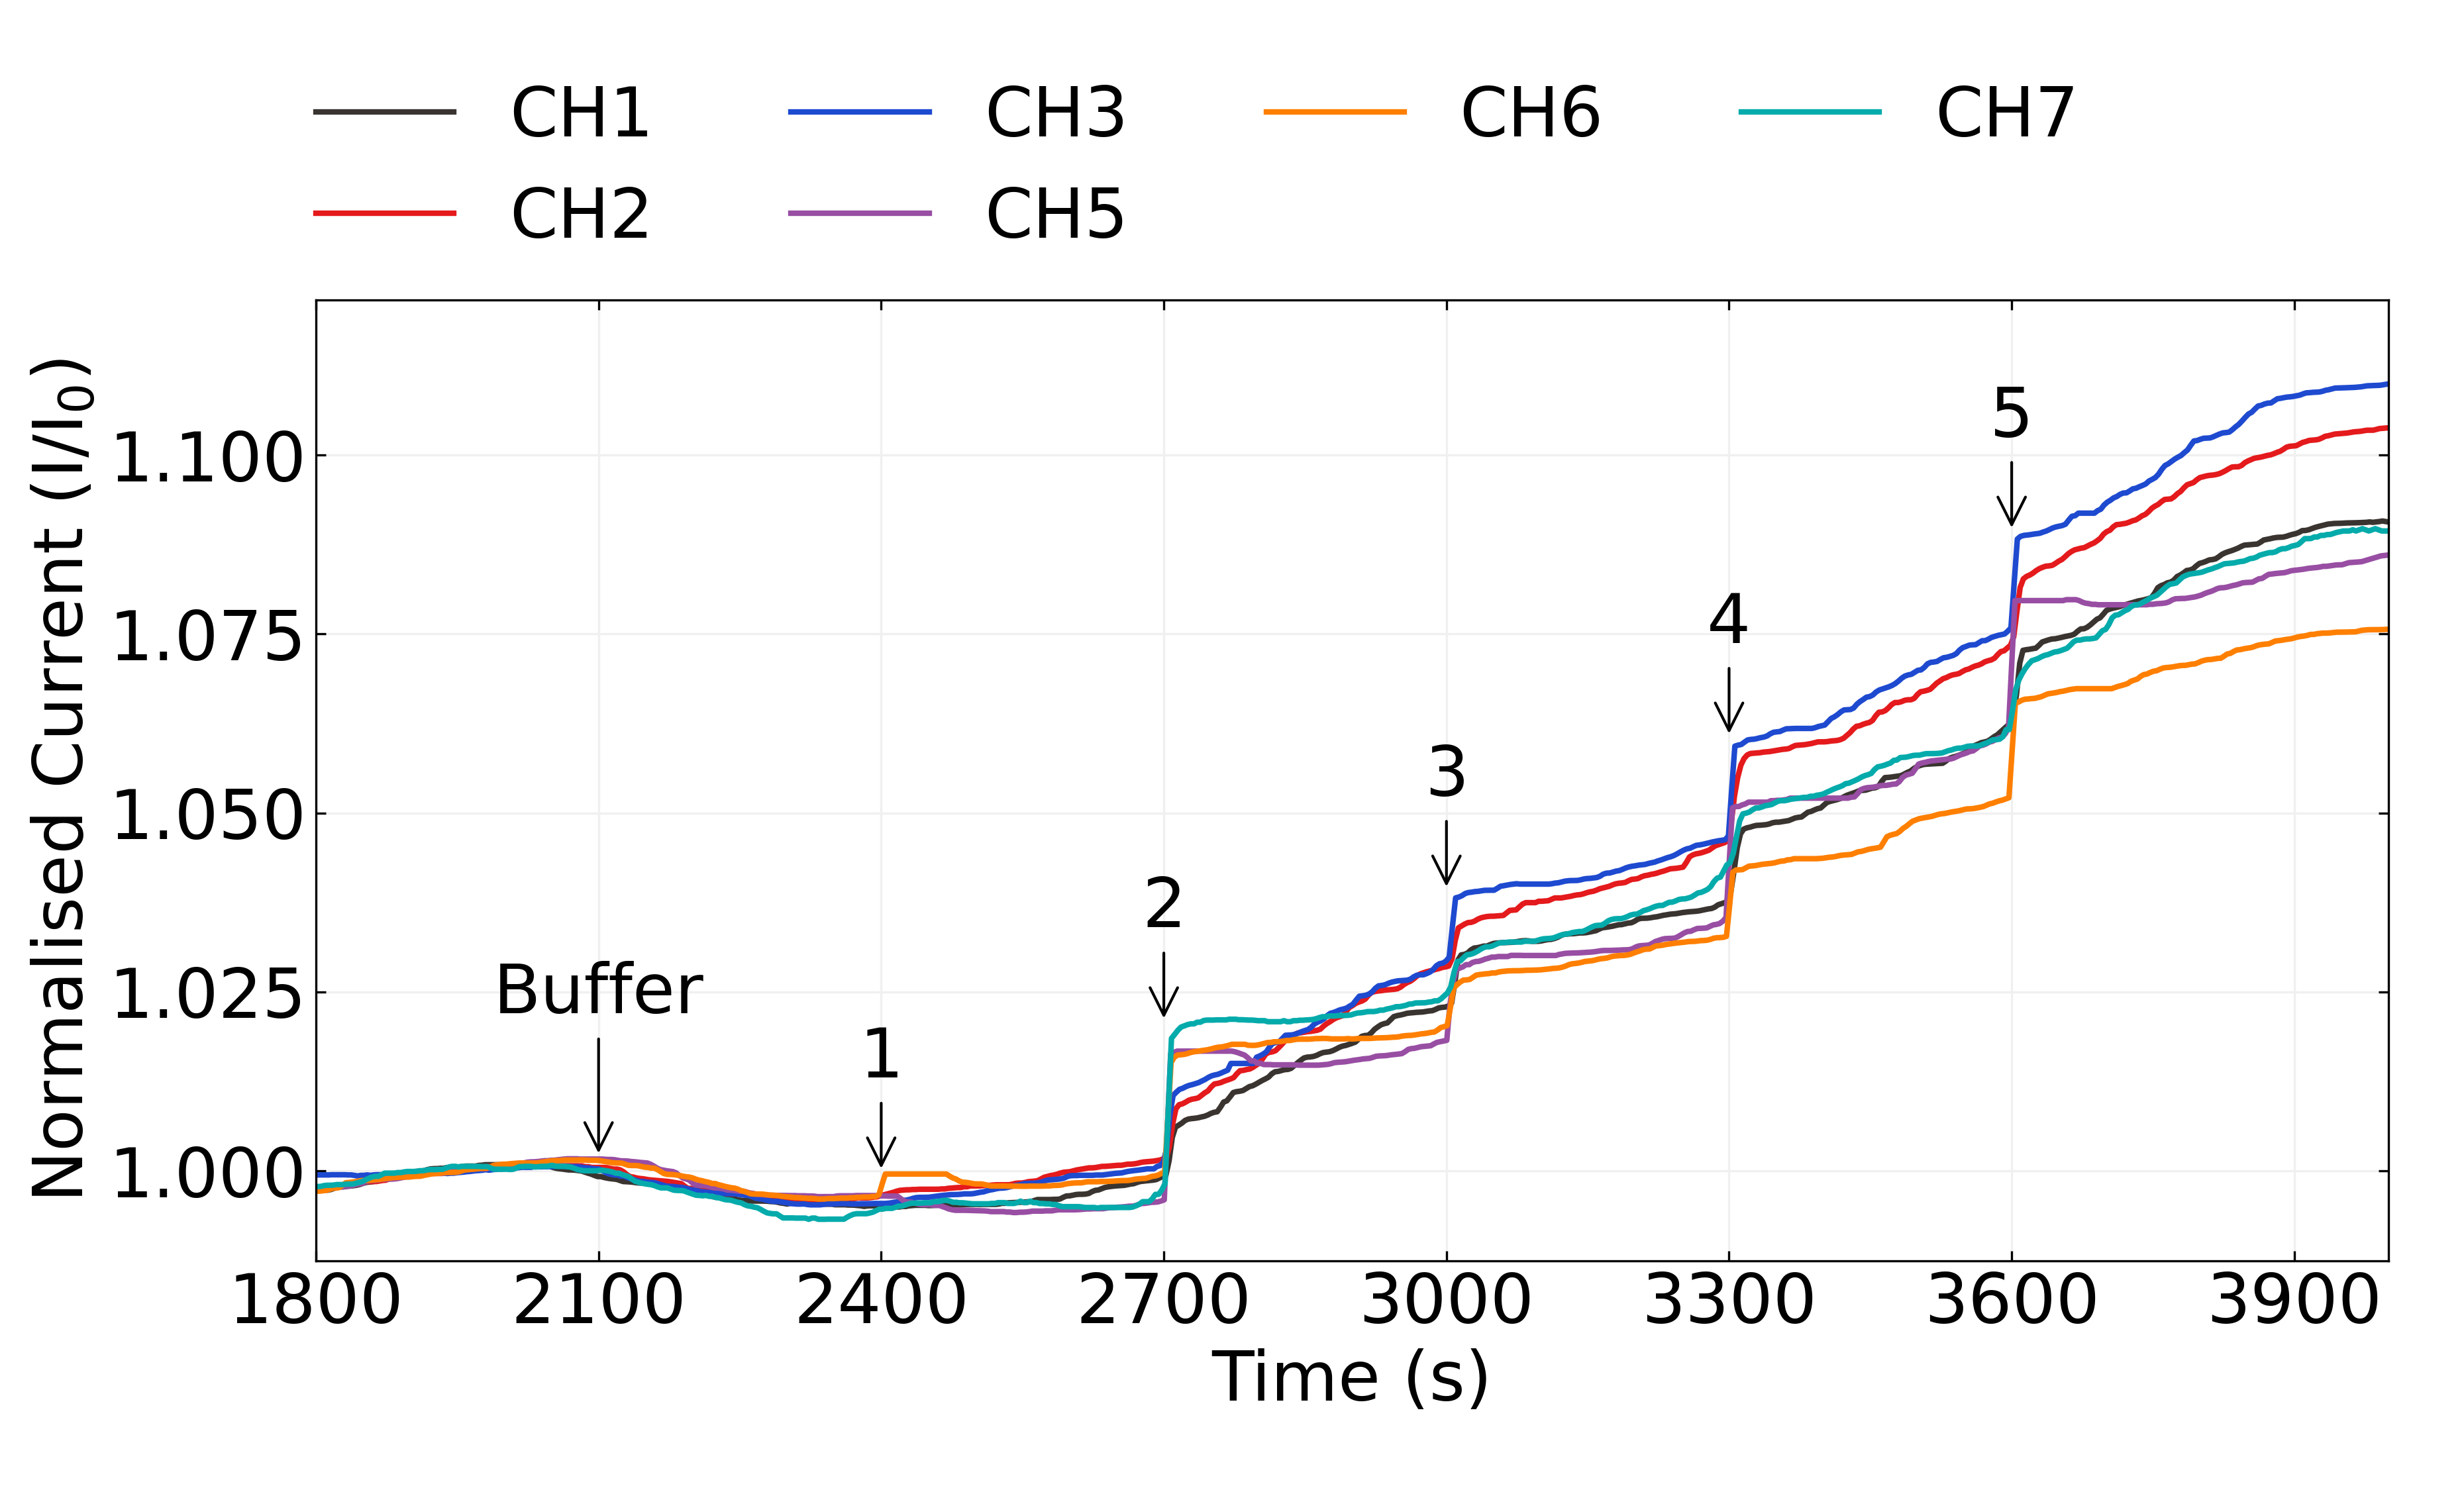
\includegraphics{figures/ch5/NTQ31C1_pristine_saltconc_sample_230324_filtered_detrend_trunc_arrows_normalised_(2).png}

}

}

\subcaption{\label{fig-salt-conc-detrend-filter}}
\end{minipage}%
%
\begin{minipage}[t]{0.50\linewidth}

{\centering 

\raisebox{-\height}{

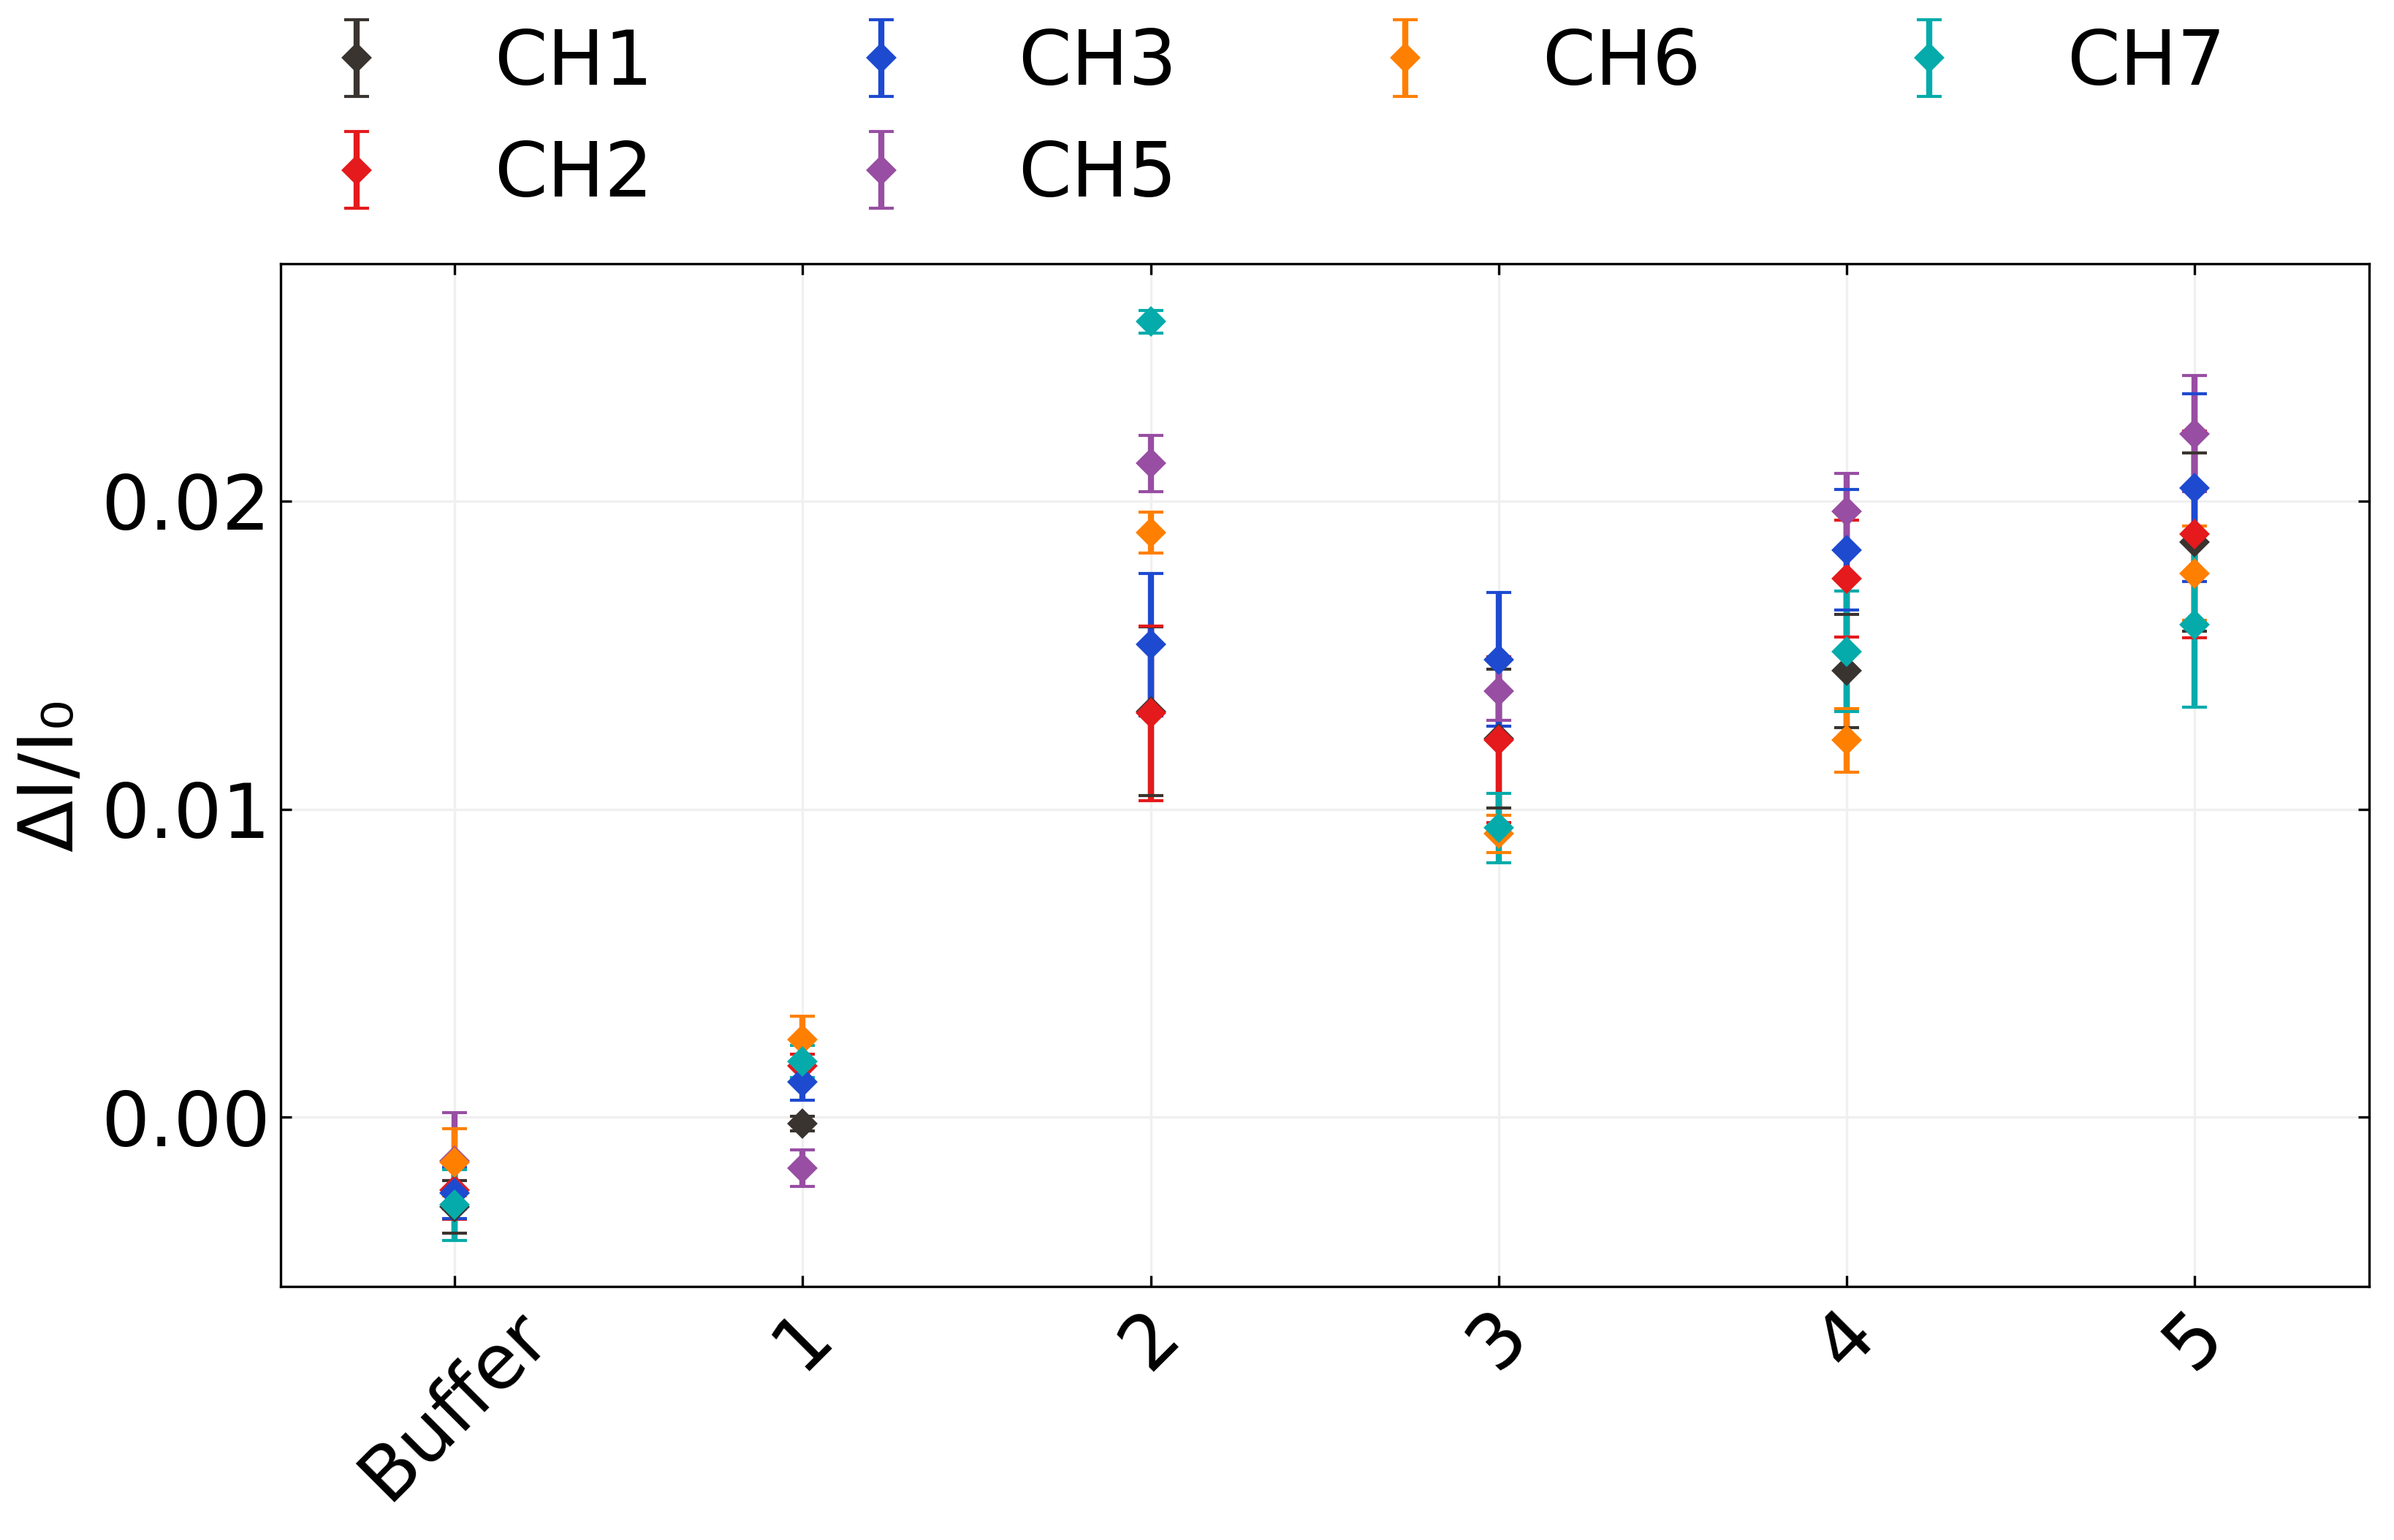
\includegraphics{figures/ch5/NTQ31C1_mean_simple_difference_before_and_after_step_filtered_concentrations.png}

}

}

\subcaption{\label{fig-salt-conc-signal}}
\end{minipage}%
\newline
\begin{minipage}[t]{0.25\linewidth}

{\centering 

~

}

\end{minipage}%
%
\begin{minipage}[t]{0.50\linewidth}

{\centering 

\raisebox{-\height}{

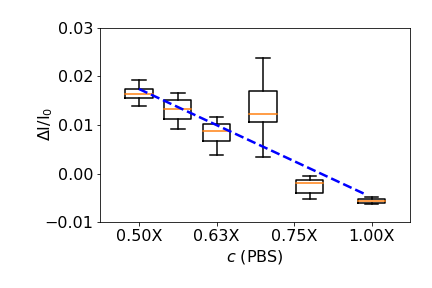
\includegraphics{figures/ch5/salt_conc_box_plot.png}

}

}

\subcaption{\label{fig-salt-conc-box-plot}}
\end{minipage}%
%
\begin{minipage}[t]{0.25\linewidth}

{\centering 

~

}

\end{minipage}%

\caption{\label{fig-salt-conc-sensing}Various visualisations of a
multiplexed salt concentration sensing series taken from a single
device. In (a), the raw current measurements for each channel are shown
alongside gate current. The same measurements after despiking, removal
of baseline drift and normalisation to initial current are shown in (b),
(c) shows the data in (b) after being processed with a moving median
filter, and (d) shows the signal changes in (c). The signal data in (d)
is shown in box plot format in (e) alongside a fit to the median change
in signal for each addition. The R squared value for the fit was 0.86.}

\end{figure}

Figure~\ref{fig-salt-conc-no-norm} shows a multiplexed salt
concentration sensing series from the channels of a single
AZ\(^\circledR\) 1518 encapsulated device, measured with the NI-PXIe.
The gate voltage used was 0.0 V; this meant current measurements were
well above the magnitude of the subthreshold device current. Gate
current measurements did not exceed 1 nA for the SU8 encapsulated
devices, and did not exceed 10 nA for the AZ\(^\circledR\) 1518 devices.
At each of the deionised water addition times, the current traces for at
least two out of six channels showed a sharp, transient increase in
current followed by a return to an increased baseline. This baseline
follows the downwards drift discussed in
Section~\ref{sec-baseline-drift}. It is well established that changing
the salt concentration of the liquid gate has an electrostatic gating
effect on the carbon nanotubes or graphene, and changes the transfer
characteristics of the channel. This shift in transfer characteristic
means we observe a realtime signal response to each addition
\autocite{Heller2009,Heller2010,Kireev2017}.

Following the discussion in Section~\ref{sec-baseline-drift}, we can
subtract the linear term approximating baseline drift (\(mt\)) for each
channel from the data in Figure~\ref{fig-salt-conc-no-norm} to account
for the downward drift. The mean current level just before 1800 s then
becomes roughly constant. We then normalise each channel relative to
their initial mean current level \(I_{0}\). We also remove artifacts
resulting from PXIe-2737 module lag, single datapoints which fall well
below the current level of the immediately preceding and succeeding
datapoints. This `despike' process uses an interquartile range filter,
as discussed in Section~\ref{sec-field-effect-transistor-analysis}. The
resulting dataset is shown in Figure~\ref{fig-salt-conc-detrend}. This
figure shows that the signal-to-noise ratio remains roughly similar
across all channels of the device. However, the behaviour of the initial
transient increase with each addition is highly variable across channels
and between additions for a single channel.

As measurement of the highly variable initial transient is not useful
for robust sensing purposes, we can apply a moving median filter to the
dataset, discussed further in
Section~\ref{sec-field-effect-transistor-analysis}. The filtered data is
shown in Figure~\ref{fig-salt-conc-detrend-filter}. Noise and initial
transients are removed completely, while the clearly defined step to a
new current baseline is retained. Using the realtime data in
Figure~\ref{fig-salt-conc-detrend-filter}, a plot of signal against
addition can be created using the method described in
Section~\ref{sec-field-effect-transistor-analysis}, shown in
Figure~\ref{fig-salt-conc-signal}. This presentation of the data allows
us to see the increase at each step relative to \(I_{0}\).

Intriguingly, even though the largest change in PBS concentration
occurred at the first deionised water addition (see
Table~\ref{tbl-salt-conc-series}), there was very little signal change
across all channels, while a relatively large change occurred at the
second addition. The logarithm of final salt concentration has
previously been shown to be proportional to conductance change in the
linear on-regime \autocite{Heller2010}.
Figure~\ref{fig-salt-conc-box-plot} shows the signal change presented in
terms of this logarithmic relationship. We see that the median values of
the first two additions do not line up well with the overall logarithmic
trend. Insufficient mixing in the tightly enclosed PDMS well environment
for the first few additions may be responsible for this result.
Subsequent additions may improve mixing in the well, leading to the
change in concentration at the surface of the channel being more
representative of the overall concentration in the well.

\begin{figure}

\begin{minipage}[t]{0.50\linewidth}

{\centering 

\raisebox{-\height}{

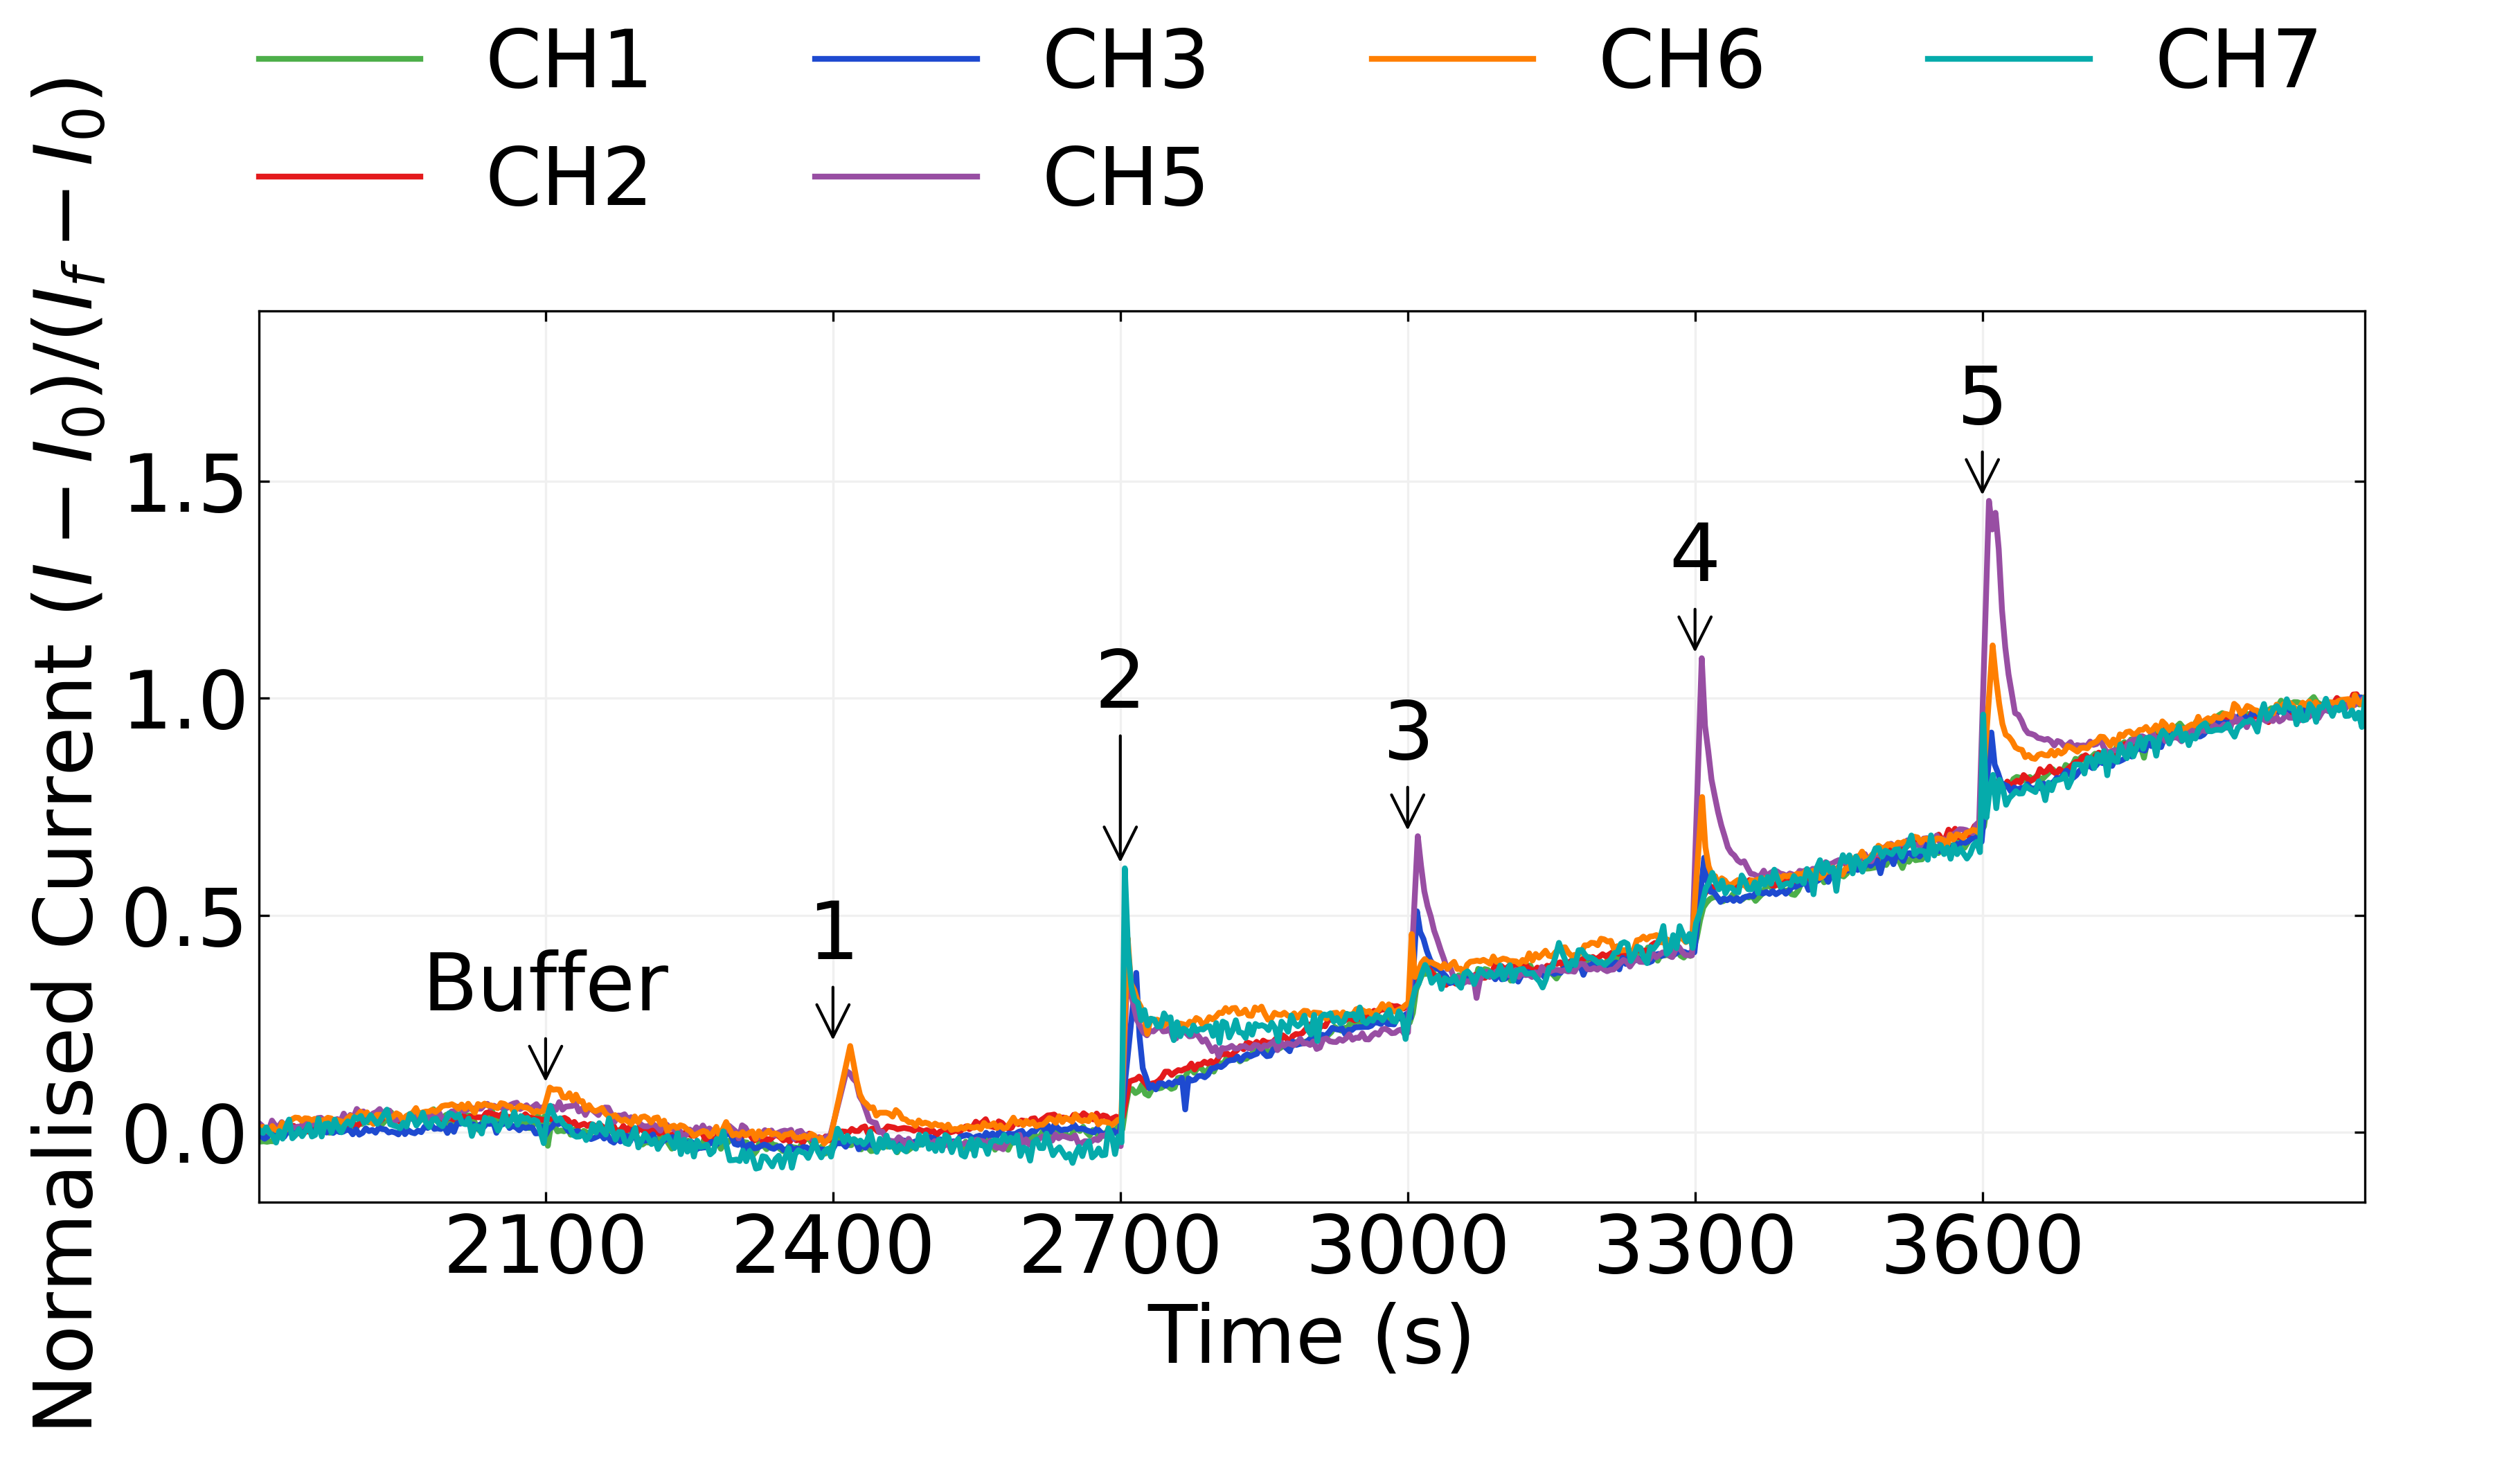
\includegraphics{figures/ch5/NTQ31C1_pristine_saltconc_sample_230324_detrend_trunc_arrows_normalised_2.png}

}

}

\subcaption{\label{fig-salt-conc-detrend-2}}
\end{minipage}%
%
\begin{minipage}[t]{0.50\linewidth}

{\centering 

\raisebox{-\height}{

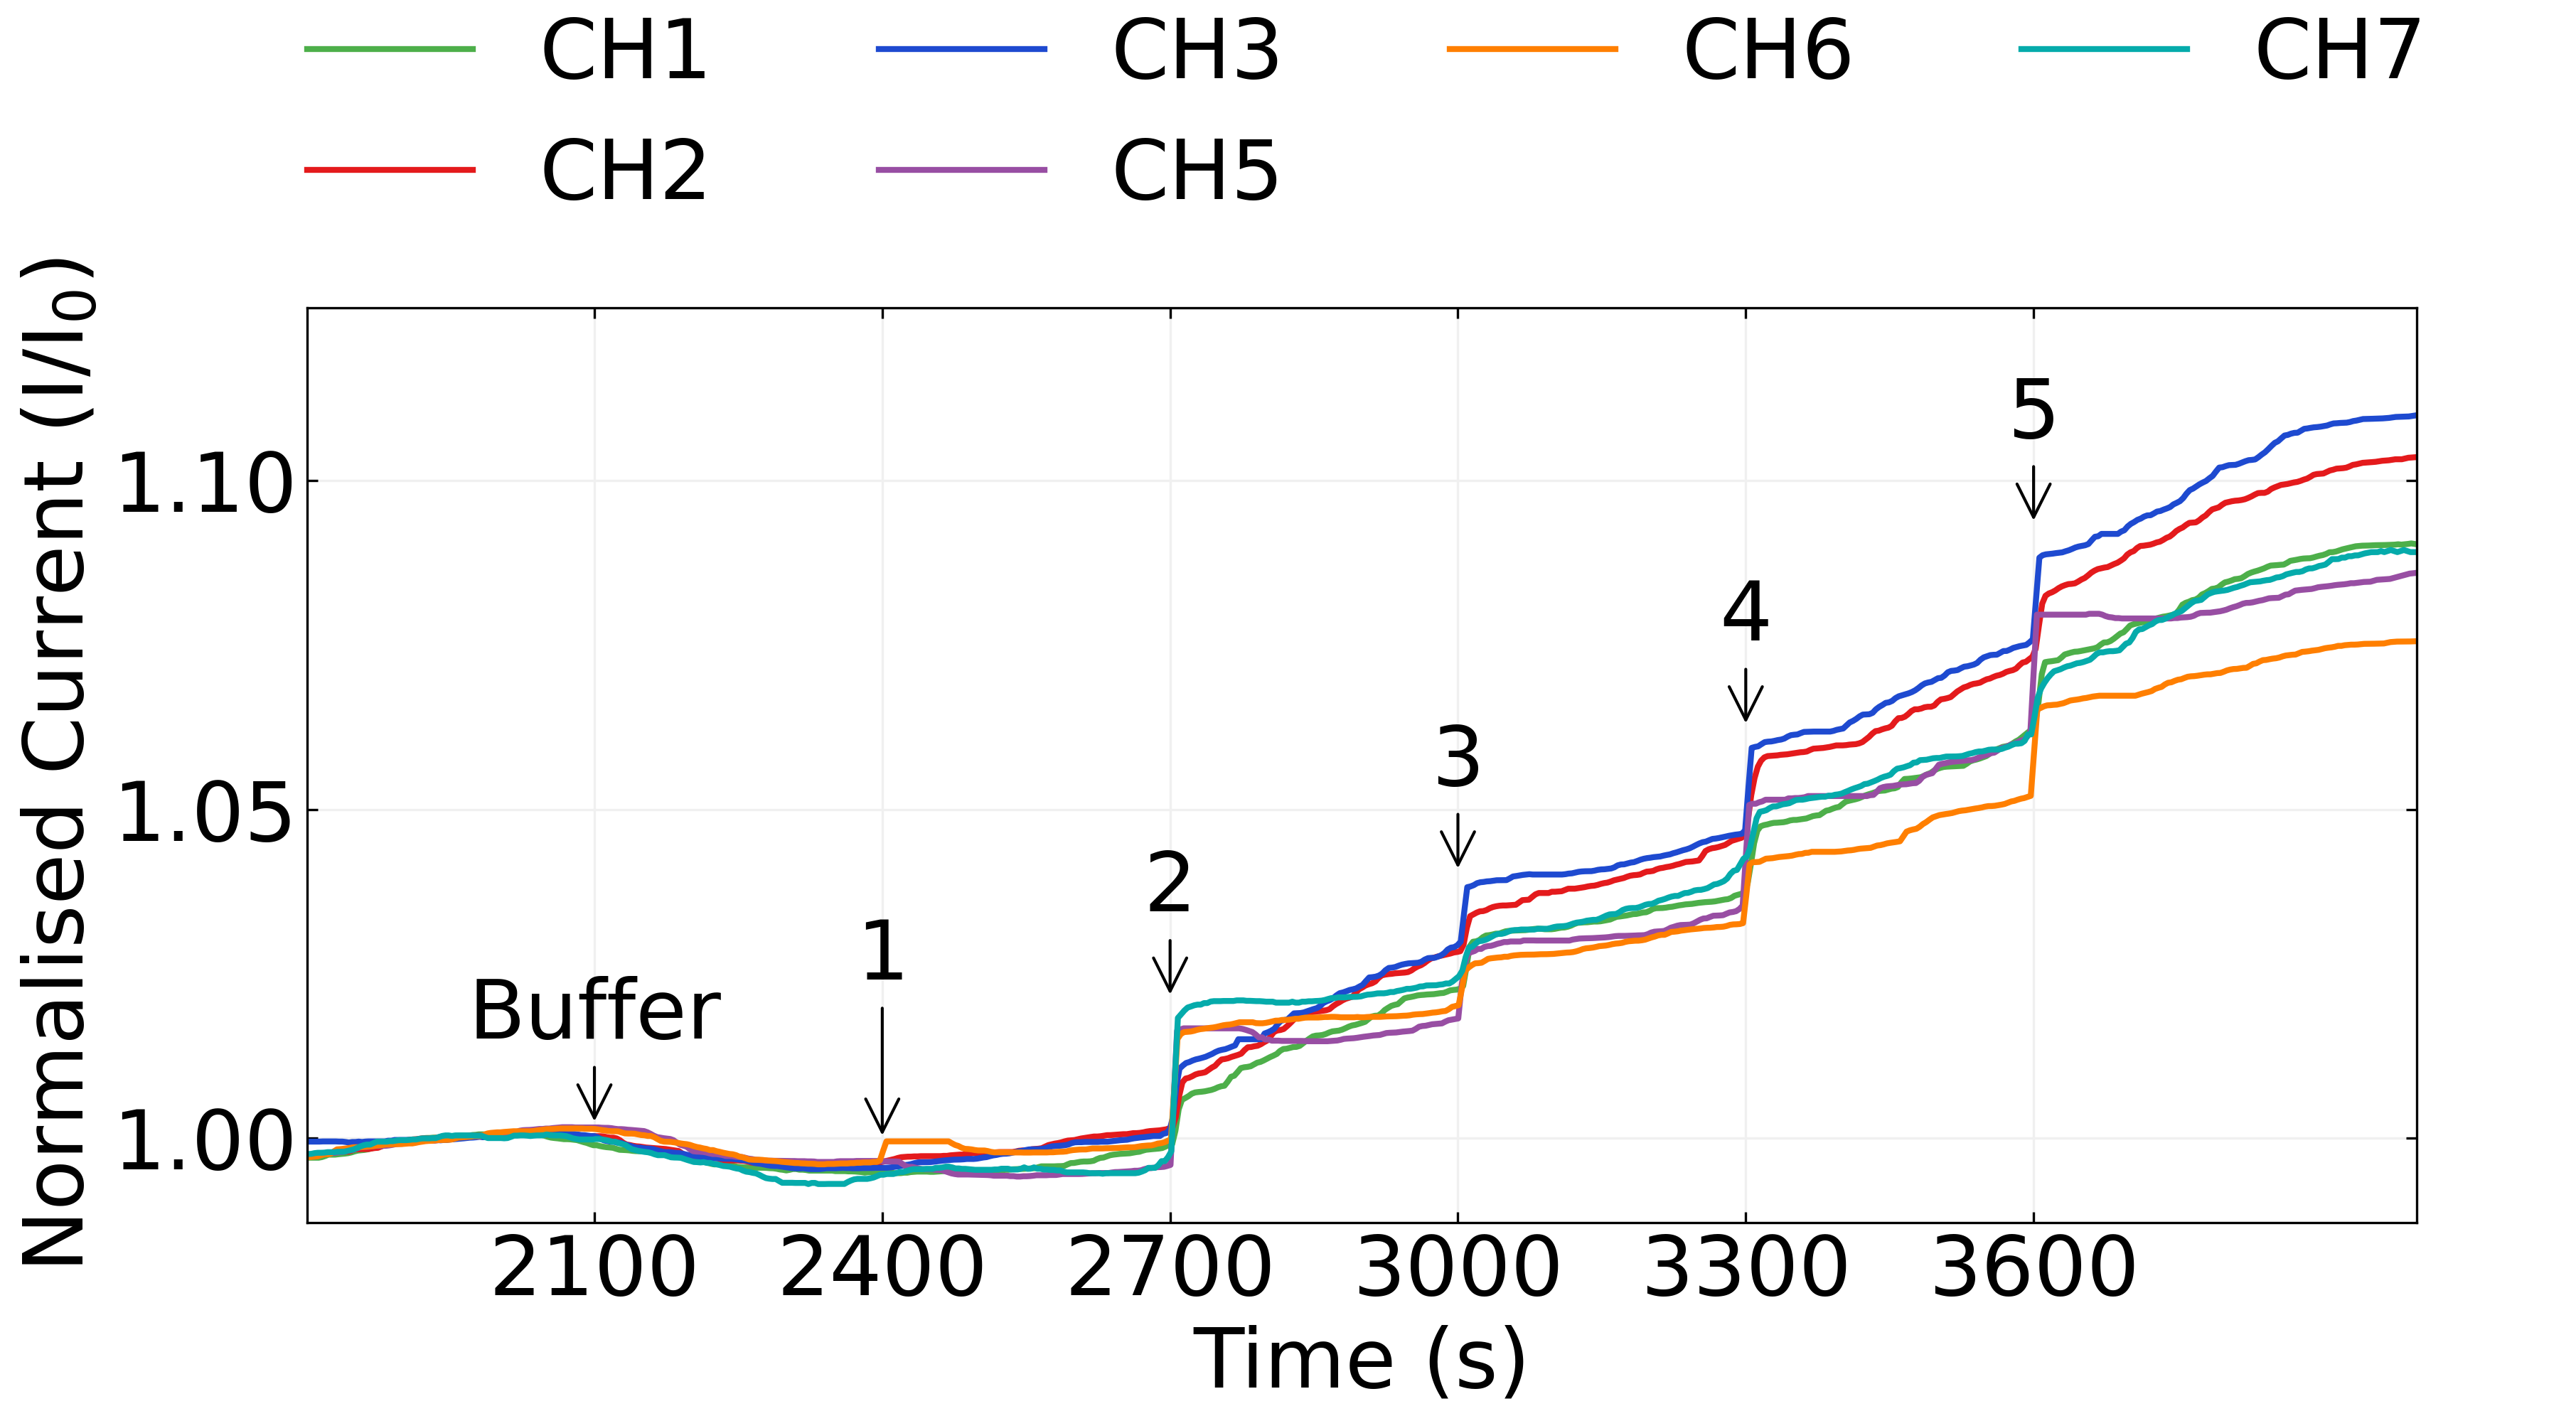
\includegraphics{figures/ch5/NTQ31C1_pristine_saltconc_sample_230324_filtered_detrend_trunc_arrows_normalised.png}

}

}

\subcaption{\label{fig-salt-conc-detrend-filter-2}}
\end{minipage}%

\caption{\label{fig-salt-conc-sensing-2}If normalised so that the size
of signal change is measured relative to the final instead of initial
current, Figure~\ref{fig-salt-conc-detrend} and
Figure~\ref{fig-salt-conc-detrend-filter} can be shown as (e) and (f)
respectively.}

\end{figure}

In Figure~\ref{fig-salt-conc-detrend} and
Figure~\ref{fig-salt-conc-detrend-filter}, we see that the drift
behaviour of individual channels begin to significantly diverge from one
another from roughly the second deionised water addition onwards. This
deviation from the baseline drift subtracted from the raw data occurs
either because the linear fit is only a first-order approximation which
weakens with time, or because the additions themselves affect the drift
behaviour. Displaying the data as discrete signal changes, as in
Figure~\ref{fig-salt-conc-signal}, is one way of excluding these
deviations (see Section~\ref{sec-field-effect-transistor-analysis}). An
alternative way of presenting the signal changes, by normalising
relative to both \(I_{0}\) and the final current reading, is shown in
Figure~\ref{fig-salt-conc-sensing-2}. This approach is useful for
comparing unaccounted-for drift behaviour as well as the initial
transient responses to additions between the channels of a multiplexed
device.

Figure~\ref{fig-salt-conc-detrend-2} demonstrates that the transient
increases are consistently largest for channels in the center of the
device, and smaller for those on the device edges (channels 1 \& 2).
This spatially-dependent behaviour may indicate responses are determined
by the location of placement of the water additions along the surface of
the electrolyte in the well. From
Figure~\ref{fig-salt-conc-detrend-filter-2}, where the transient
responses are largely filtered out, we see clearly that the signal
response relative to drift is highly consistent between channels. This
result demonstrates that once unaccounted-for drift behaviour is
removed, the signal size in response to each addition is highly
consistent between channels. Slight deviations from the overall trend,
such as for channels 5, 6 and 7 at deionised water addition 2, and for
channels 5 and 6 at deionised water addition 5, are likely due to the
large transient spikes at these channels not being completely filtered
out by the median filter.

\hypertarget{signal-to-noise-ratio}{%
\subsubsection*{Signal-to-Noise Ratio}\label{signal-to-noise-ratio}}
\addcontentsline{toc}{subsubsection}{Signal-to-Noise Ratio}

\begin{figure}

\begin{minipage}[t]{0.50\linewidth}

{\centering 

\raisebox{-\height}{

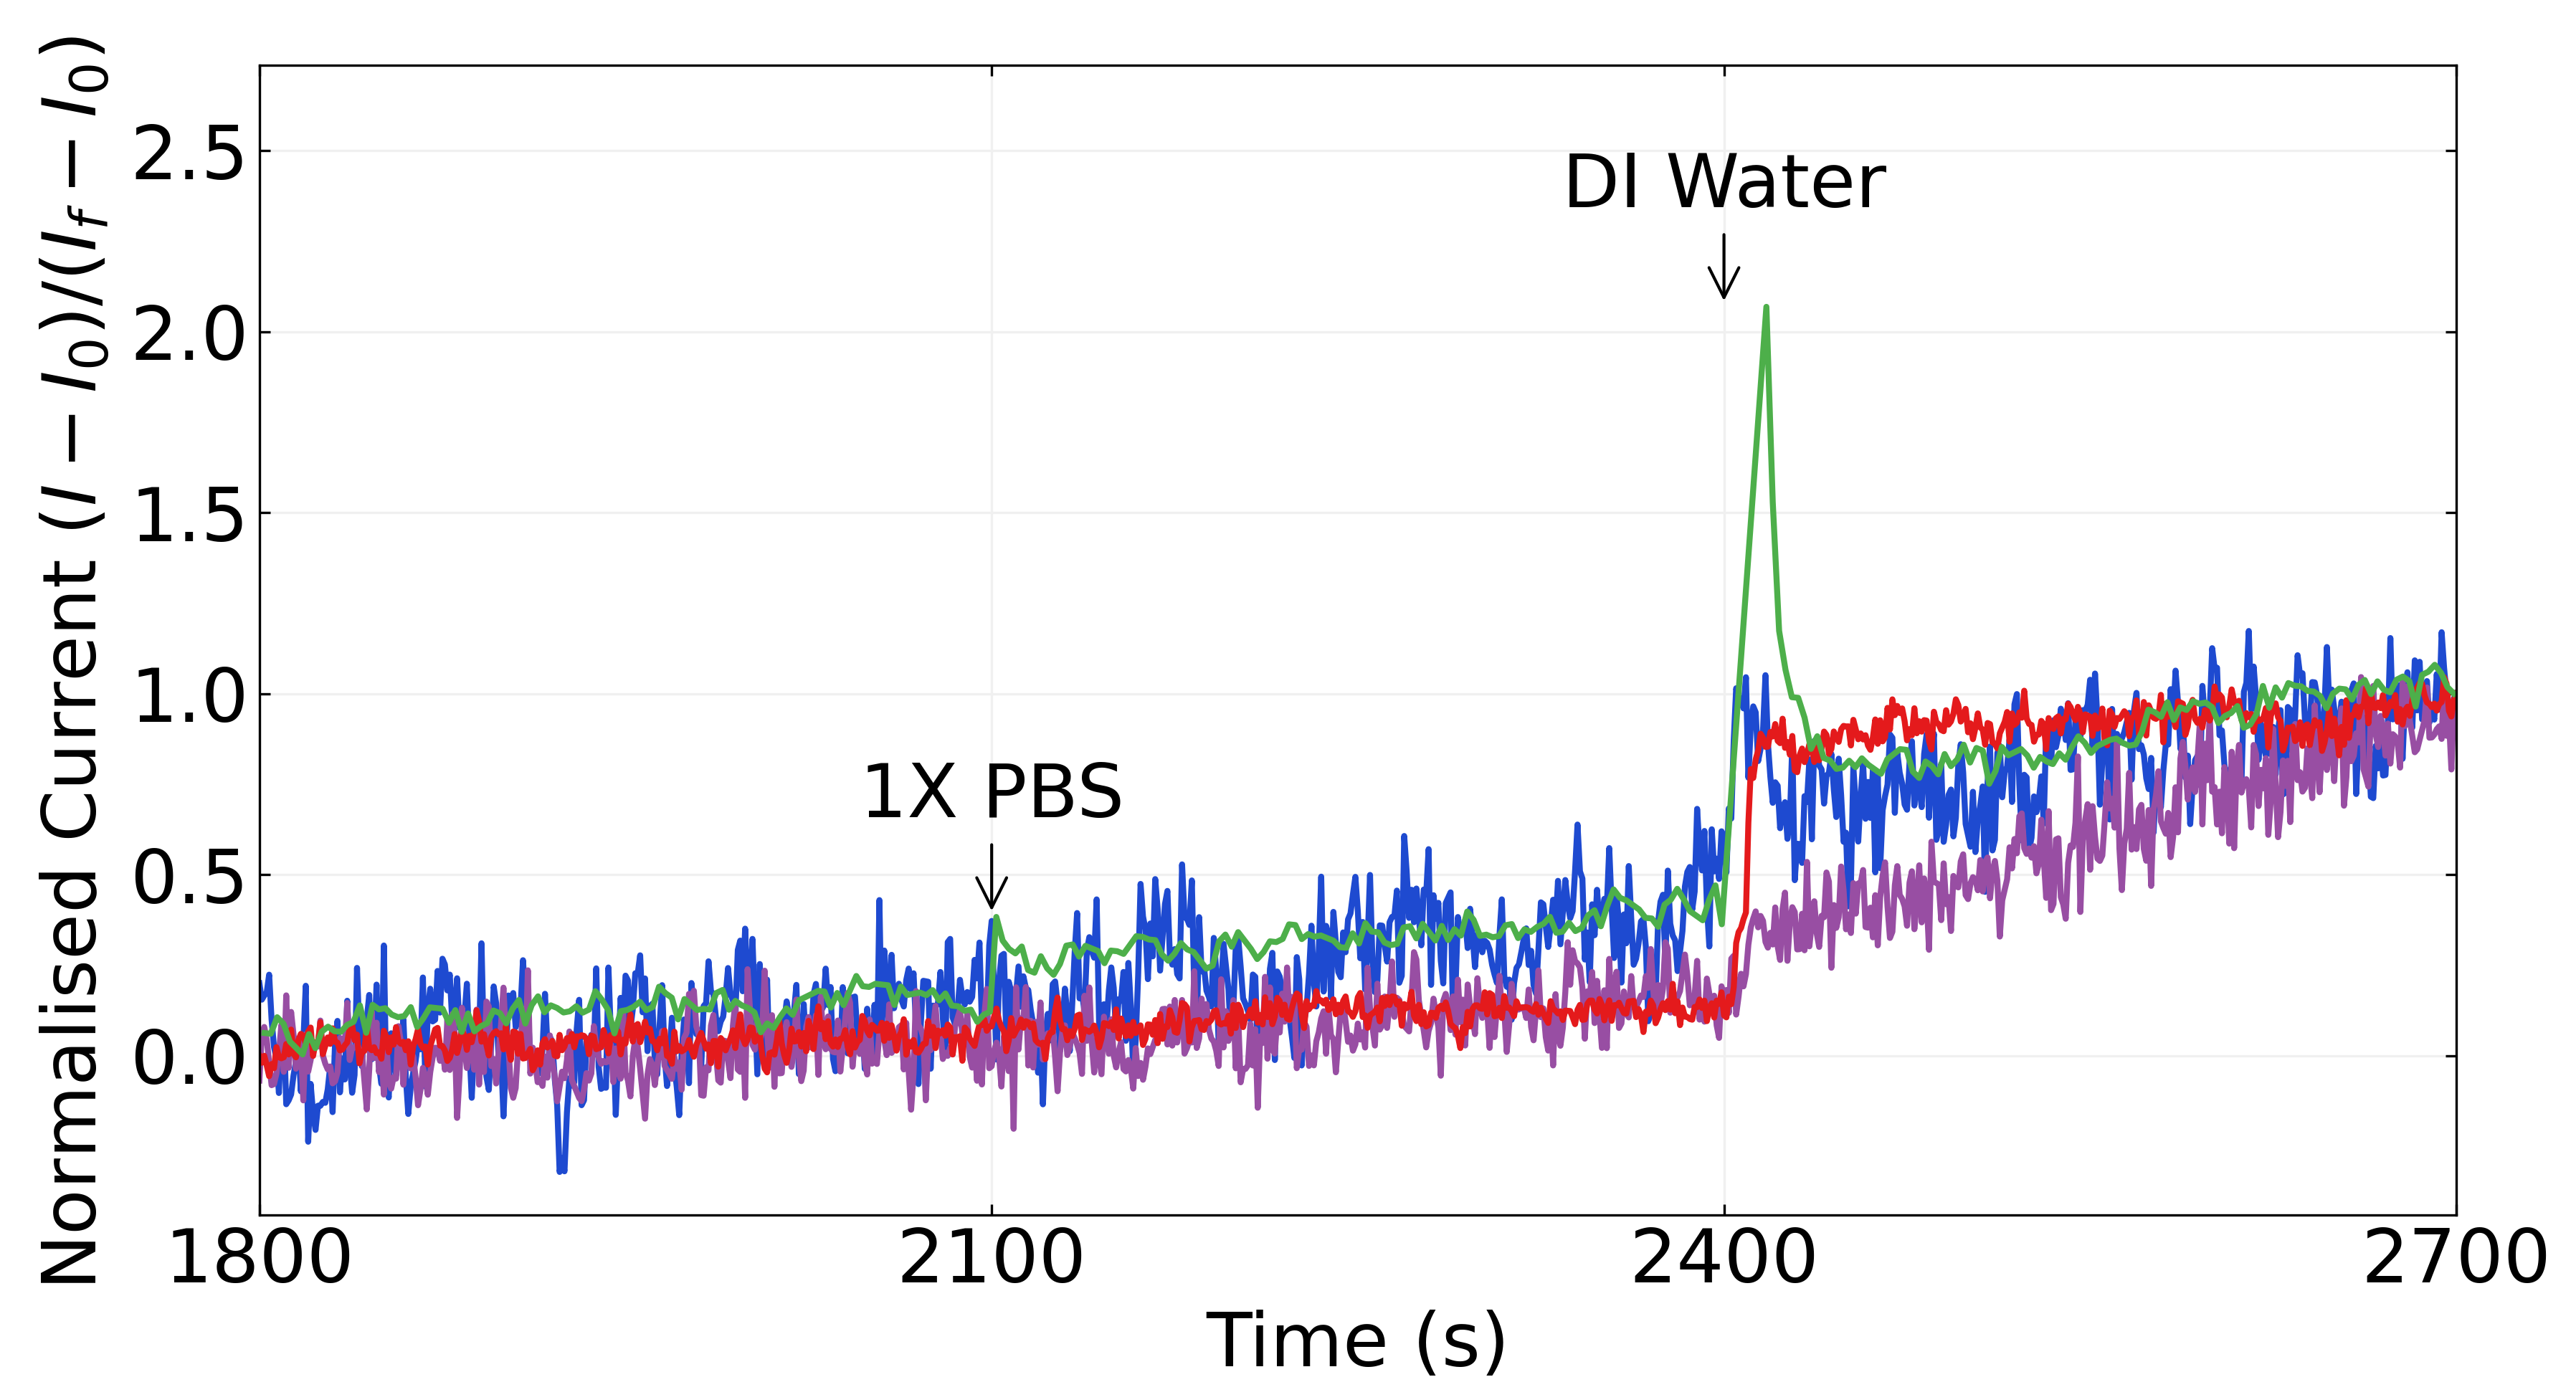
\includegraphics{figures/ch5/saltconc_initial_additions.png}

}

}

\subcaption{\label{fig-salt-conc-SNR}}
\end{minipage}%
%
\begin{minipage}[t]{0.05\linewidth}

{\centering 

~

}

\end{minipage}%
%
\begin{minipage}[t]{0.45\linewidth}

{\centering 

\raisebox{-\height}{

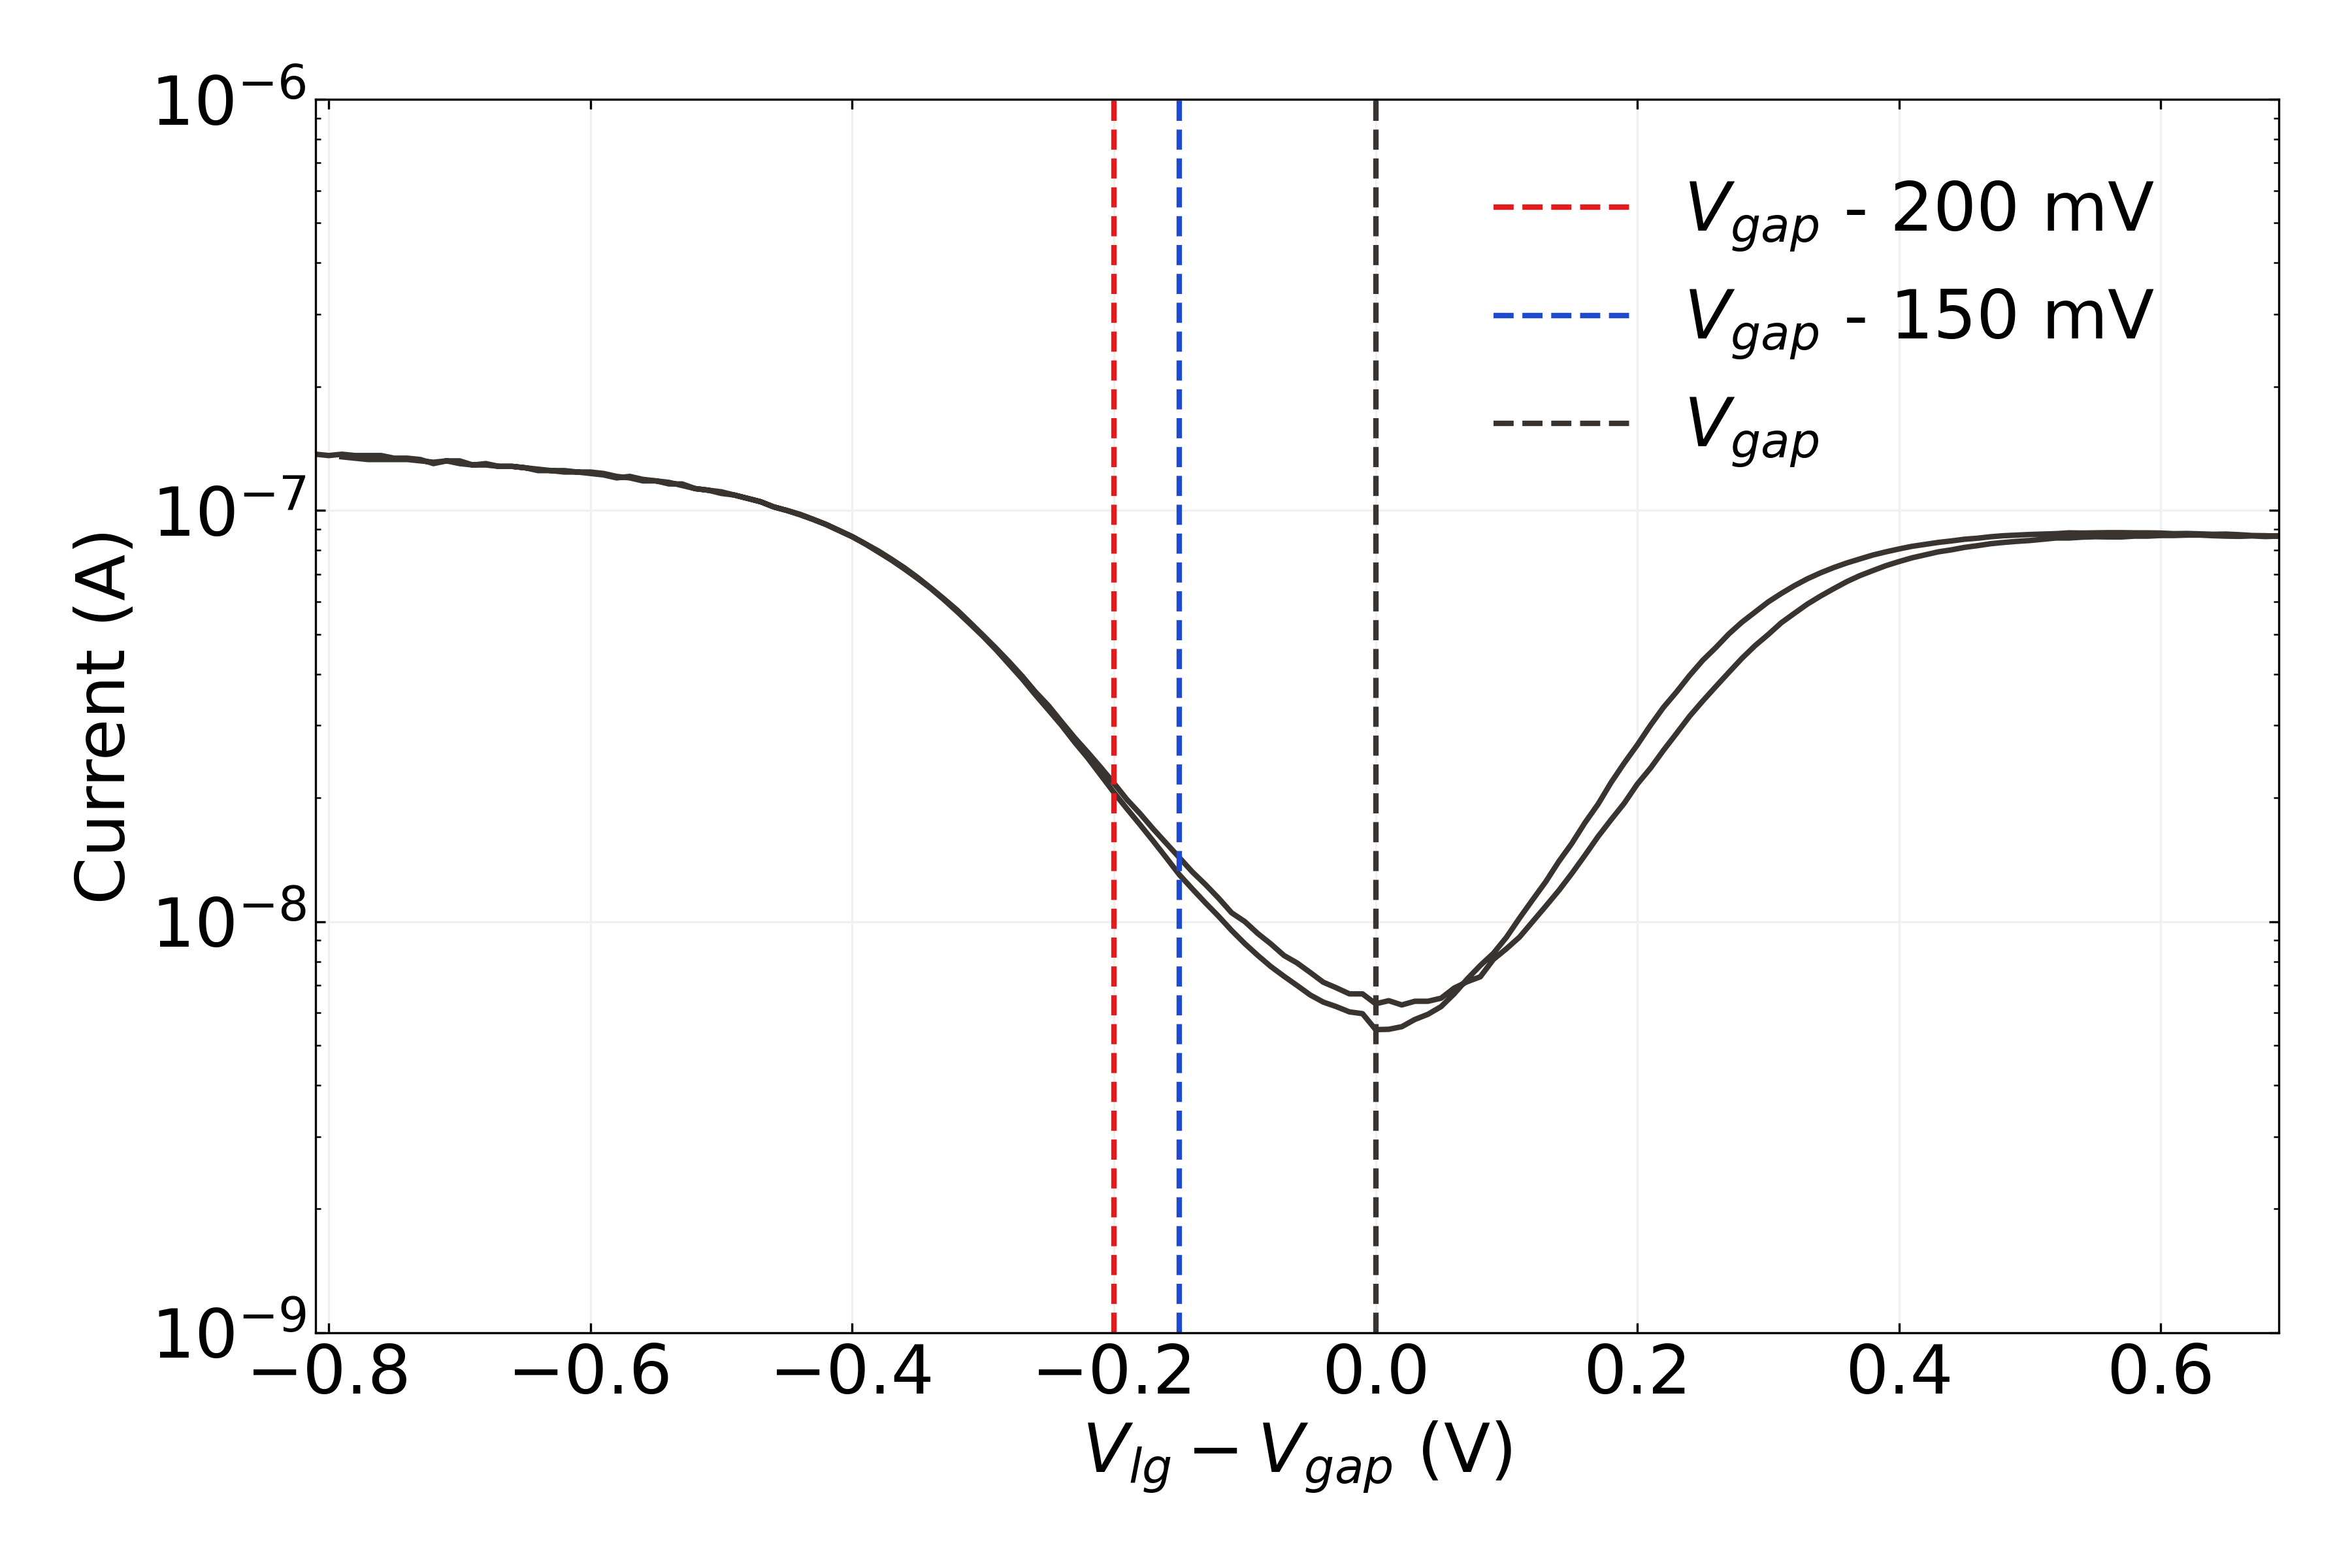
\includegraphics{figures/ch5/Q2C10ch8custom.png}

}

}

\subcaption{\label{fig-transfer-sweep-2}}
\end{minipage}%

\caption{\label{fig-salt-conc-SNR}The signal-to-noise ratio of the first
deionised water addition for the traces seen in
Figure~\ref{fig-salt-conc-control-series-SU8} are shown in (a). For
convenience, the transfer characteristics of the three channels in
Figure~\ref{fig-salt-conc-control-series-SU8}, showing the two gate
voltages used for measurements of a single SU8-encapsulated channel, are
shown again in (b).}

\end{figure}

To compare signal-to-noise ratio between different gate currents and
device configurations, the initial additions post-1800 s from the
current traces in Figure~\ref{fig-salt-conc-control-series-SU8} that
were discussed earlier in Section~\ref{sec-baseline-drift} are shown in
Figure~\ref{fig-salt-conc-SNR}. Previous work on the signal-to-noise
ratio for liquid-gated, encapsulated carbon nanotube devices suggests
that gating devices close to \(V_{gap}\) should give the largest
signal-to-noise ratio for salt concentration additions
\autocite{Heller2009}. However, as shown by
Figure~\ref{fig-salt-conc-control-series-SU8}, this relationship was not
consistently observed. This discrepancy could be a result of the use of
a network of carbon nanotubes rather than a single nanotube; gating may
have less of an impact on noise when a network morphology is used.
Alternatively, it could be a result of a lack of mixing in our static
well setup leading to inconsistent signal sizes with concentration
change. Heller \emph{et al.} used a flow cell during their
signal-to-ratio work \autocite{Heller2009}.

\hypertarget{conclusion}{%
\section{Conclusion}\label{conclusion}}

To ensure fabricated transistors were suitable for biosensing purposes,
the morphology and electrical properties of the pristine carbon nanotube
and graphene transistors were investigated.

The morphology of the carbon nanotube networks were found to have a
significant impact on the electrical characteristics of the devices,
which was determined through comparison of the height profile of the
carbon nanotube network and the key electrical parameters of a range of
carbon nanotube devices. When networks were highly bundled (\(>90\) \%),
there was a large range of carbon nanotube bundle diameters present in
the network. This large variation in the size of conducting pathways
resulted in a wide range of on-off ratios and threshold voltages for the
liquid-gated devices created using these carbon nanotube films. In
contrast, devices using films fabricated with a relatively low
percentage of bundling (\(<75\) \%) showed highly consistent on-off
ratios and threshold voltages, along with low hysteresis, due to the
relatively consistent bundle diameters and high density of these
networks. These low-bundling networks were found to have a mean bundle
distribution height of \(3.2 \pm 1.1\) nm. When performing multiplexed
sensing, consistent channel behaviour is highly desirable since
comparing sensing behaviour between channels is more straightforward.

However, atomic force microscope images of low bundling networks also
indicated that these networks have the most contamination present on the
surface of the film relative to carbon nanotubes. This is possibly the
cause of the increased threshold voltage of devices with films deposited
with steam present relative to those using films fabricated without
steam. The steam deposition may introduce \(p\)-dopants to the carbon
nanotubes, which could be due to surfactant left over from the
deposition process. Since the presence of surfactant could negatively
impact biosensing, techniques to remove contaminants should be explored
in more detail. Thermal annealing of carbon nanotube films at high
temperature is one approach that could be taken to resolve this issue,
which is discussed further in \textbf{?@sec-future-work}. The presence
of electrolyte on the surface of a backgated transistor was also found
to significantly adversely affect its electrical characteristics.

Constant voltage real-time measurements of the carbon nanotube devices
had a characteristic drift that could be modelled using a exponential
and linear term. The linear term of baseline drift appeared to be
characteristic to the type of device measured, where the equation of the
trendline for linear drift was proportionally related between channels
fabricated in the same manner. An increase in device current level
therefore meant an increase in the degree of linear drift. The time
constant of the exponential term appeared to be characteristic to the
particular channel used, with a time constant of \(\tau = 300 \pm 20\) s
for the SU8-encapsulated channel characteristed, and time constants of
\(\tau = 141 \pm 3\) s and \(\tau = 408 \pm 11\) s for the
AZ\(^\circledR\) 1518 devices characterised.

Salt concentration sensing series indicated that the carbon nanotube
transistor devices were highly sensitive to environmental changes and
therefore suitable for sensing work. Successive additions of deionised
water to the 1X PBS present in the well gave signal responses of up to
2.5 \% above the control response. The signal response was found to be
proportional to the logarithm of concentration, giving a fit to the
median response sizes with an \(R^2 = 0.86\). Deviations from this trend
can possibly be explained by the enclosed sensing environment preventing
sufficient mixing of electrolyte concentrations within the PDMS well. It
was also seen that the relative signal size to baseline drift was highly
consistent between channels. This is a promising result when it comes to
ensuring consistent multiplexin, but it remains to be seen if this
behaviour carries over to sensing with biofunctionalised devices.

Graphene devices were often found to possess a double-minima feature,
which appears to be the result of a lack of doping from the metal
contacts in the center of the device channels. These double Dirac points
are unlikely to have an significant effect on the sensing behaviour of
graphene devices. The graphene device characteristics were found to be
consistent after 1 hour exposure to 1X PBS with minimal drift, with an
on-off ratio of 5 and major Dirac point voltage of 0.3 V. There was some
indications from the transfer characteristics that \(p\)-dopants were
present on the graphene surface.

\cleardoublepage
\phantomsection
\addcontentsline{toc}{part}{Appendices}
\appendix

\hypertarget{sec-python}{%
\chapter{Python Code for Data Analysis}\label{sec-python}}

\hypertarget{code-repository}{%
\section{Code Repository}\label{code-repository}}

The code used for general analysis of field-effect transistor devices in
this thesis was written with Python 3.8.8. Contributors to the code used
include Erica Cassie, Erica Happe, Marissa Dierkes and Leo Browning. The
code is located on GitHub and the research group OneDrive, and is
available on request.

\hypertarget{sec-histogram-analysis}{%
\section{Atomic Force Microscope Histogram
Analysis}\label{sec-histogram-analysis}}

The purpose of this code is to analyse atomic force microscope (AFM)
images of carbon nanotube networks in .xyz format taken using an atomic
force microscope and processed in Gwyddion (see
\textbf{?@sec-afm-characterisation}). It was originally designed by
Erica Happe in Matlab, and adapted by Marissa Dierkes and myself for use
in Python.

\begin{equation}\protect\hypertarget{eq-lin-combo-gaussian}{}{
f(x) = k_1\exp{\Bigg(-\frac{{(x-m_1)}^{2}}{{2s_1}^{2}}\Bigg)} + k_2\exp{\Bigg(-\frac{{(x-m_2)}^{2}}{{2s_2}^{2}}\Bigg)} + ...
}\label{eq-lin-combo-gaussian}\end{equation}

The .xyz data is initially sorted into bins with 0.15 nm size. The bin
with the maximum number of counts is set at 0 nm, as this peak
represents the mean of the surface roughness of the bare silicon. The
parameters \(m_i\), \(s_i\), \(k_i\) (i = 1, 2, 3) are used with
objective function Equation~\ref{eq-lin-combo-gaussian} to overlay the
data with normal distributions. These fitting parameters represent the
mean (m), standard deviation (s) and amplitude (k) of each normal
distribution. We can make approximations of some of these fitting
parameters using the histogram data.

\(k_1\) is taken to be the maximum y-value of the data being fitted,
\(m_1\) is set to zero (used as a point of reference) and \(s_1\) is
taken as one-third of the difference between \(m_1\) and the x-value of
the first datapoint where the y-value is greater than 1\% of \(k_1\)
(approximating one standard deviation). We find the distribution given
by these values using Equation~\ref{eq-lin-combo-gaussian}, and subtract
it from the existing dataset.

The code also allows for discretely binning continuous data from fitted
normal distributions and examining the proportion of counts above or
below a particular height. 2.9 nm is roughly where 2 bundles with
average size 1.45 nm can start to be present, and is used as an estimate
of the boundary value between single-tube bundle diameters and
multi-tube bundle diameters.

\hypertarget{sec-raman-analysis}{%
\section{Raman Spectroscopy Analysis}\label{sec-raman-analysis}}

The purpose of this code is to analyse a series of Raman spectra taken
at different points on a single film (see
\textbf{?@sec-raman-characterisation}).

Data is imported in a tab-delimited text file, and the baseline region
between 1400 and 1500 cm\(^{-1}\) is set as zero amplitude for data
collected from each film location. The data from each location is then
normalised to the D-peak (the maximum point on the D-peak, which lies
between 1300 and 1400 cm\(^{-1}\), is set equal to unity). Using these
datasets, plots of normalised intensity relative to the D-peak comparing
each location can be created. The ratio I\(^{D}\)/I\(_{G}\) can be found
by taking the inverse of the maximum point on the G-peak of these
normalised plots. A plot of the average intensity across all locations
measured can also be created.

\hypertarget{sec-field-effect-transistor-analysis}{%
\section{Field-Effect Transistor
Analysis}\label{sec-field-effect-transistor-analysis}}

The purpose of this code is to analyse electrical measurements taken of
field-effect transistor (FET) devices. Electrical measurements were
either taken from the Keysight 4156C Semiconductor Parameter Analyser,
National Instruments NI-PXIe or Keysight B1500A Semiconductor Device
Analyser as discussed in \textbf{?@sec-electrical-characterisation}; the
code is able to analyse data taken from all three measurement setups.
The main Python file in the code base consists of three related but
independent modules: the first analyses and plots sensing data from the
FET devices, the second analyses and plots transfer characteristics from
channels across a device, and the third compares individual channel
characteristics before and after a modification or after each of several
modifications. The code base also features a separate config file and
style sheet which govern the behaviour of the main code. The code base
was designed collaboratively by myself and Erica Cassie over GitHub
using the Sourcetree Git GUI.

The first of the three modules is for processing sensing datasets. This
module imports sensing measurements in .csv format and analyses them,
then outputs a plot of the raw data, alongside multiple plots which have
been modified in various ways. It can also fit exponential and linear
trendlines to regions of the sensing data, as well as find the signal
change per analyte addition, and returns spreadsheets containing the
results of these analyses. These spreadsheets include the standard
deviation for all included parameters. Modified plots include normalised
plots (type of normalisation can be set in config file), plots with
fitted curves, plots with the linear baseline drift removed, plots of
signal with analyte addition, ``despiked'' plots and ``filtered'' plots.
It is possible to add annotations to any of these plots using the config
file, and it is possible to produce a plot with a combination of these
modifications.

The scipy.optimize.curve\_fit module is used to fit linear and
exponential curves to regions of interest of the sensing data. Initial
parameters for the scipy.optimize.curve\_fit module are chosen by
approximating fitting parameters in a similar manner to the approach in
Section~\ref{sec-histogram-analysis}. For a linear fit \(mt + b\), the
parameters are simply set as \(m=1\) and \(b=0\). For an exponential fit
\(a\exp{(-t/\tau)} + c\), \(c\) is set as the final current measurement
of the region of interest and \(a\) is set as the initial current
measurement minus \(c\). Then, \(\tau\) is set as the time where current
has dropped to \(e^{-1}a + c\).

``Despiked'' plots have had spurious datapoints removed through the use
of an interquartile range rolling filter. The window size of the rolling
filter used was 40 datapoints, and datapoints in each window with a
z-score above \(\pm 3\) were removed from the plotted/processed data.
``Filtered'' plots had noise reduced using a moving median filter. The
moving median filter is more effective at removing noise than a simple
moving average, and has advantages over other filters (such as the
Savitzky-Golay filter) when removing noise from data with sharp edges,
as is the case for sensing data. Median filtering can also be used for
baseline drift compensation, though this approach was not used in this
thesis \autocite{Stone2011}. The moving median filter used had a window
of 40 datapoints.

Plots of signal with analyte addition were constructed from current data
after first removing baseline drift and applying a moving median filter.
A simple difference calculation between the mean of the filtered current
before an addition and the mean of the filtered current after the
addition was performed at each addition. These differences were then
normalised relative to the initial current. The signal with analyte
addition give reasonably consistent results regardless of whether
baseline drift was removed from the data, as shown in
Figure~\ref{fig-spaa-plot-comparison}. We can therefore be confident
that robust signal with analyte addition plots are robust even in the
presence of significant drift.

\begin{figure}

\begin{minipage}[t]{0.50\linewidth}

{\centering 

\raisebox{-\height}{

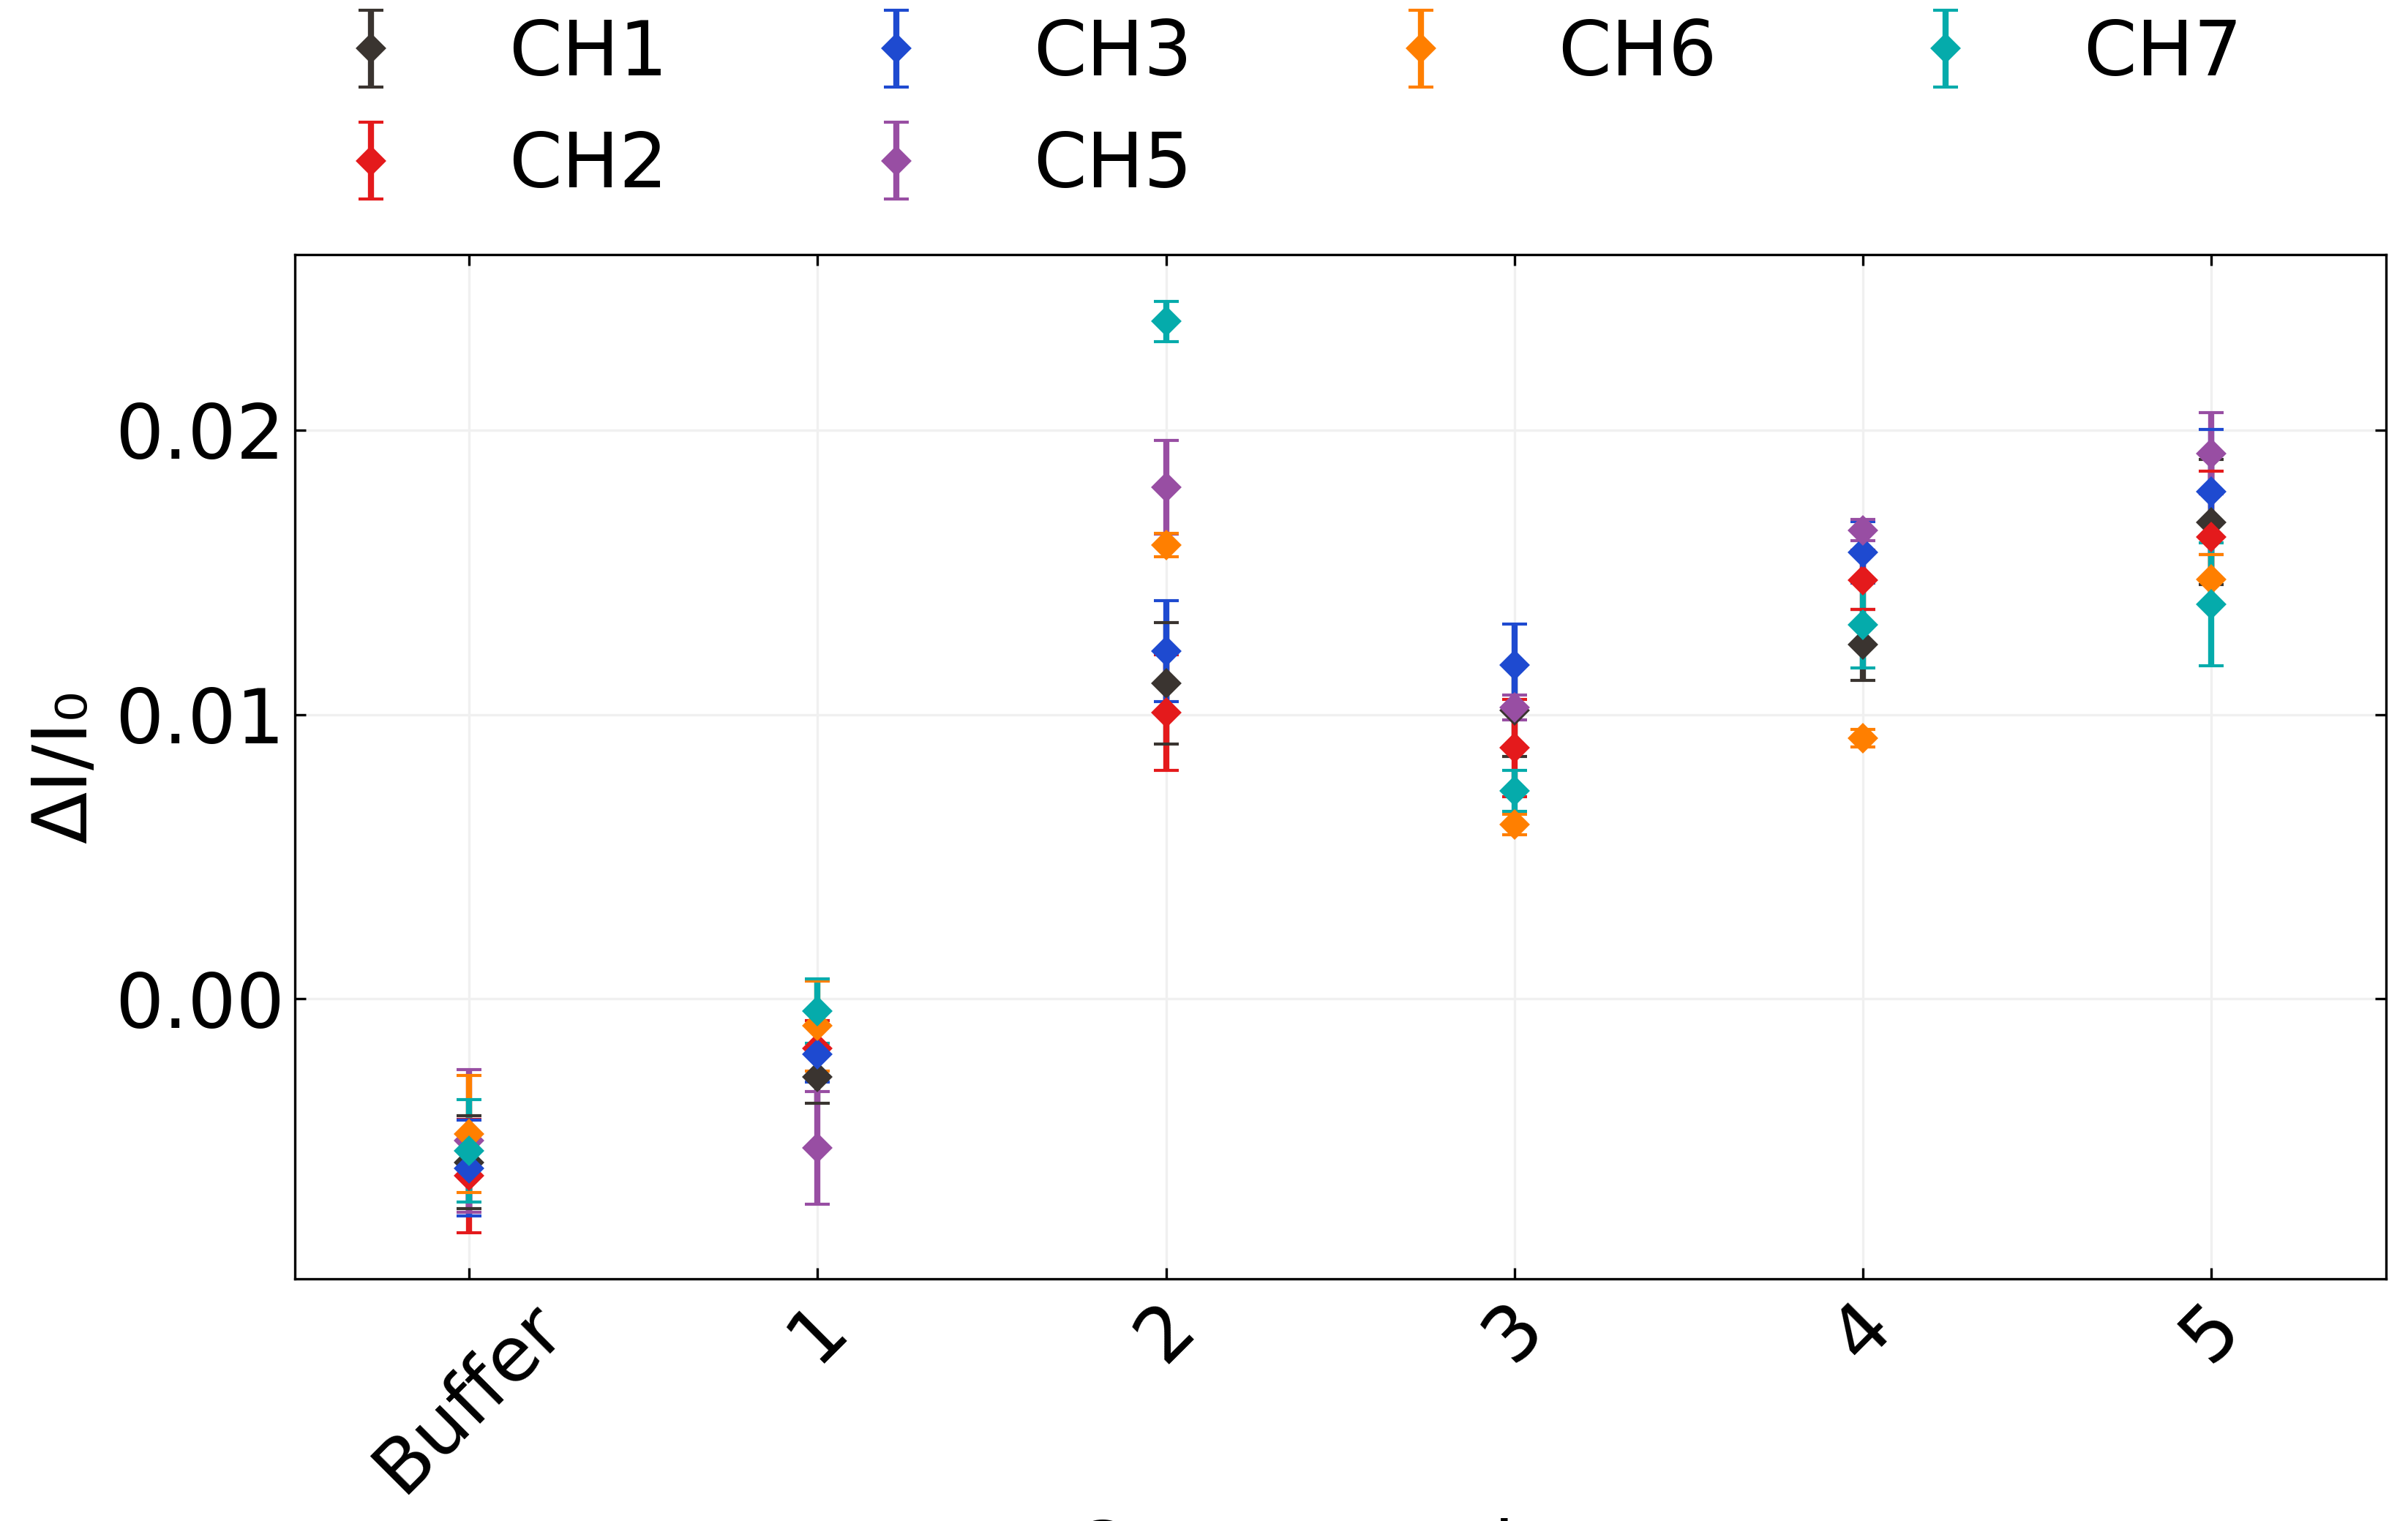
\includegraphics{figures/app1/NTQ31C1_mean_simple_difference_before_and_after_step_filtered_concentrations.png}

}

}

\subcaption{\label{fig-spaa-no-detrend}}
\end{minipage}%
%
\begin{minipage}[t]{0.50\linewidth}

{\centering 

\raisebox{-\height}{

\includegraphics{figures/app1/NTQ31C1_mean_simple_difference_before_and_after_step_filtered_concentrations_detrend.png}

}

}

\subcaption{\label{fig-spaa-detrend}}
\end{minipage}%

\caption{\label{fig-spaa-plot-comparison}A comparison of signal with
analyte addition plots taken from the same salt concentration sensing
dataset (the same dataset as used in
Figure~\ref{fig-salt-conc-sensing}). In (a), a simple difference
calculation performed on filtered data was used, while in (b) the same
calculation was performed on filtered data with the baseline drift
removed, the method used in the body of the thesis.}

\end{figure}

The second module imports transfer measurements in .csv format and
creates combined and individual plots of the eight channels on a single
device. In combined plots, channels which are non-working, due to being
shorted or non-conducting, are removed via setting a maximum and minimum
possible on-current in the config file. Various parameters from the
transfer characteristics are saved as a spreadsheet along with standard
error. These parameters include on current, off current, subthreshold
slope and threshold voltage for the carbon nanotube devices, and on
current, off current and major Dirac point voltage for graphene devices.
The device type being analysed can be set in the config file.

The third module imports several transfer measurements in .csv format
and allows for comparison of the same channel before and after some
modification. It also calculates the shift in either threshold voltage
or major Dirac voltage of the device.


\backmatter
\printbibliography


\end{document}
